\documentclass[twoside]{book}

% Packages required by doxygen
\usepackage{fixltx2e}
\usepackage{calc}
\usepackage{doxygen}
\usepackage[export]{adjustbox} % also loads graphicx
\usepackage{graphicx}
\usepackage[utf8]{inputenc}
\usepackage{makeidx}
\usepackage{multicol}
\usepackage{multirow}
\PassOptionsToPackage{warn}{textcomp}
\usepackage{textcomp}
\usepackage[nointegrals]{wasysym}
\usepackage[table]{xcolor}

% Font selection
\usepackage[T1]{fontenc}
\usepackage[scaled=.90]{helvet}
\usepackage{courier}
\usepackage{amssymb}
\usepackage{sectsty}
\renewcommand{\familydefault}{\sfdefault}
\allsectionsfont{%
  \fontseries{bc}\selectfont%
  \color{darkgray}%
}
\renewcommand{\DoxyLabelFont}{%
  \fontseries{bc}\selectfont%
  \color{darkgray}%
}
\newcommand{\+}{\discretionary{\mbox{\scriptsize$\hookleftarrow$}}{}{}}

% Page & text layout
\usepackage{geometry}
\geometry{%
  a4paper,%
  top=2.5cm,%
  bottom=2.5cm,%
  left=2.5cm,%
  right=2.5cm%
}
\tolerance=750
\hfuzz=15pt
\hbadness=750
\setlength{\emergencystretch}{15pt}
\setlength{\parindent}{0cm}
\setlength{\parskip}{3ex plus 2ex minus 2ex}
\makeatletter
\renewcommand{\paragraph}{%
  \@startsection{paragraph}{4}{0ex}{-1.0ex}{1.0ex}{%
    \normalfont\normalsize\bfseries\SS@parafont%
  }%
}
\renewcommand{\subparagraph}{%
  \@startsection{subparagraph}{5}{0ex}{-1.0ex}{1.0ex}{%
    \normalfont\normalsize\bfseries\SS@subparafont%
  }%
}
\makeatother

% Headers & footers
\usepackage{fancyhdr}
\pagestyle{fancyplain}
\fancyhead[LE]{\fancyplain{}{\bfseries\thepage}}
\fancyhead[CE]{\fancyplain{}{}}
\fancyhead[RE]{\fancyplain{}{\bfseries\leftmark}}
\fancyhead[LO]{\fancyplain{}{\bfseries\rightmark}}
\fancyhead[CO]{\fancyplain{}{}}
\fancyhead[RO]{\fancyplain{}{\bfseries\thepage}}
\fancyfoot[LE]{\fancyplain{}{}}
\fancyfoot[CE]{\fancyplain{}{}}
\fancyfoot[RE]{\fancyplain{}{\bfseries\scriptsize Generated by Doxygen }}
\fancyfoot[LO]{\fancyplain{}{\bfseries\scriptsize Generated by Doxygen }}
\fancyfoot[CO]{\fancyplain{}{}}
\fancyfoot[RO]{\fancyplain{}{}}
\renewcommand{\footrulewidth}{0.4pt}
\renewcommand{\chaptermark}[1]{%
  \markboth{#1}{}%
}
\renewcommand{\sectionmark}[1]{%
  \markright{\thesection\ #1}%
}

% Indices & bibliography
\usepackage{natbib}
\usepackage[titles]{tocloft}
\setcounter{tocdepth}{3}
\setcounter{secnumdepth}{5}
\makeindex

% Hyperlinks (required, but should be loaded last)
\usepackage{ifpdf}
\ifpdf
  \usepackage[pdftex,pagebackref=true]{hyperref}
\else
  \usepackage[ps2pdf,pagebackref=true]{hyperref}
\fi
\hypersetup{%
  colorlinks=true,%
  linkcolor=blue,%
  citecolor=blue,%
  unicode%
}

% Custom commands
\newcommand{\clearemptydoublepage}{%
  \newpage{\pagestyle{empty}\cleardoublepage}%
}

\usepackage{caption}
\captionsetup{labelsep=space,justification=centering,font={bf},singlelinecheck=off,skip=4pt,position=top}

%===== C O N T E N T S =====

\begin{document}

% Titlepage & ToC
\hypersetup{pageanchor=false,
             bookmarksnumbered=true,
             pdfencoding=unicode
            }
\pagenumbering{alph}
\begin{titlepage}
\vspace*{7cm}
\begin{center}%
{\Large My Project }\\
\vspace*{1cm}
{\large Generated by Doxygen 1.8.13}\\
\end{center}
\end{titlepage}
\clearemptydoublepage
\pagenumbering{roman}
\tableofcontents
\clearemptydoublepage
\pagenumbering{arabic}
\hypersetup{pageanchor=true}

%--- Begin generated contents ---
\chapter{lib\+Multi\+Robot\+Planning}
\label{index}\hypertarget{index}{}This library contains implementations of search algorithms in C++(14). The library is header only and uses templates.

\subsection*{Supported Algorithms}

\subsubsection*{Single-\/\+Robot}

\tabulinesep=1mm
\begin{longtabu} spread 0pt [c]{*{2}{|X[-1]}|}
\hline
\rowcolor{\tableheadbgcolor}\textbf{ Algorithm }&\textbf{ Optimality  }\\\cline{1-2}
\endfirsthead
\hline
\endfoot
\hline
\rowcolor{\tableheadbgcolor}\textbf{ Algorithm }&\textbf{ Optimality  }\\\cline{1-2}
\endhead
\hyperlink{classlib_multi_robot_planning_1_1_a_star}{A$\ast$} &optimal \\\cline{1-2}
\hyperlink{classlib_multi_robot_planning_1_1_a_star_epsilon}{A$\ast$\+\_\+epsilon} &w-\/bounded suboptimal \\\cline{1-2}
S\+I\+PP &optimal \\\cline{1-2}
\end{longtabu}
\subsubsection*{Multi-\/\+Robot}

\tabulinesep=1mm
\begin{longtabu} spread 0pt [c]{*{2}{|X[-1]}|}
\hline
\rowcolor{\tableheadbgcolor}\textbf{ Algorithm }&\textbf{ Optimality  }\\\cline{1-2}
\endfirsthead
\hline
\endfoot
\hline
\rowcolor{\tableheadbgcolor}\textbf{ Algorithm }&\textbf{ Optimality  }\\\cline{1-2}
\endhead
\hyperlink{classlib_multi_robot_planning_1_1_c_b_s}{Conflict-\/\+Based Search (C\+BS)} &optimal (sum-\/of-\/cost) \\\cline{1-2}
\hyperlink{classlib_multi_robot_planning_1_1_e_c_b_s}{Enhanced Conflict-\/\+Based Search (E\+C\+BS)} &w-\/bounded suboptimal (sum-\/of-\/cost) \\\cline{1-2}
Conflict-\/\+Based Search with Optimal Task Assignment (C\+B\+S-\/\+TA) &optimal (sum-\/of-\/cost) \\\cline{1-2}
Enhanced Conflict-\/\+Based Search with Optimal Task Assignment (E\+C\+B\+S-\/\+TA) &w-\/bounded suboptimal (sum-\/of-\/cost) \\\cline{1-2}
\mbox{[}Prioritized Planning with S\+I\+PP\mbox{]} &No \\\cline{1-2}
\end{longtabu}
\subsubsection*{Assignment}

\tabulinesep=1mm
\begin{longtabu} spread 0pt [c]{*{2}{|X[-1]}|}
\hline
\rowcolor{\tableheadbgcolor}\textbf{ Algorithm }&\textbf{ Optimality  }\\\cline{1-2}
\endfirsthead
\hline
\endfoot
\hline
\rowcolor{\tableheadbgcolor}\textbf{ Algorithm }&\textbf{ Optimality  }\\\cline{1-2}
\endhead
Best Assignment (Network flow based) &optimal (sum-\/of-\/cost) \\\cline{1-2}
Next Best Assignment &series of optimal solutions (sum-\/of-\/cost) \\\cline{1-2}
\end{longtabu}

\chapter{Namespace Index}
\section{Namespace List}
Here is a list of all namespaces with brief descriptions\+:\begin{DoxyCompactList}
\item\contentsline{section}{\hyperlink{namespace__setup__util}{\+\_\+setup\+\_\+util} }{\pageref{namespace__setup__util}}{}
\item\contentsline{section}{\hyperlink{namespacegenerate__cached__setup}{generate\+\_\+cached\+\_\+setup} }{\pageref{namespacegenerate__cached__setup}}{}
\item\contentsline{section}{\hyperlink{namespacelib_corridor_gen}{lib\+Corridor\+Gen} }{\pageref{namespacelib_corridor_gen}}{}
\item\contentsline{section}{\hyperlink{namespacelib_multi_robot_planning}{lib\+Multi\+Robot\+Planning} }{\pageref{namespacelib_multi_robot_planning}}{}
\item\contentsline{section}{\hyperlink{namespacepkg}{pkg} }{\pageref{namespacepkg}}{}
\item\contentsline{section}{\hyperlink{namespacestd}{std} }{\pageref{namespacestd}}{}
\end{DoxyCompactList}

\chapter{Hierarchical Index}
\section{Class Hierarchy}
This inheritance list is sorted roughly, but not completely, alphabetically\+:\begin{DoxyCompactList}
\item \contentsline{section}{lib\+Multi\+Robot\+Planning\+:\+:A\+Star$<$ State, Action, Cost, Environment, State\+Hasher $>$}{\pageref{classlib_multi_robot_planning_1_1_a_star}}{}
\item \contentsline{section}{lib\+Multi\+Robot\+Planning\+:\+:A\+Star\+Epsilon$<$ State, Action, Cost, Environment, State\+Hasher $>$}{\pageref{classlib_multi_robot_planning_1_1_a_star_epsilon}}{}
\item \contentsline{section}{Box\+Constraint2D}{\pageref{struct_box_constraint2_d}}{}
\item \contentsline{section}{lib\+Multi\+Robot\+Planning\+:\+:C\+BS$<$ State, Action, Cost, Conflict, Constraints, Environment $>$}{\pageref{classlib_multi_robot_planning_1_1_c_b_s}}{}
\item \contentsline{section}{Conflict}{\pageref{struct_conflict}}{}
\item \contentsline{section}{lib\+Multi\+Robot\+Planning\+:\+:Conflict}{\pageref{structlib_multi_robot_planning_1_1_conflict}}{}
\item \contentsline{section}{Constraints}{\pageref{struct_constraints}}{}
\item \contentsline{section}{lib\+Multi\+Robot\+Planning\+:\+:Constraints}{\pageref{structlib_multi_robot_planning_1_1_constraints}}{}
\item \contentsline{section}{lib\+Corridor\+Gen\+:\+:Corridor}{\pageref{classlib_corridor_gen_1_1_corridor}}{}
\item \contentsline{section}{Corridor2D}{\pageref{struct_corridor2_d}}{}
\item \contentsline{section}{lib\+Multi\+Robot\+Planning\+:\+:E\+C\+BS$<$ State, Action, Cost, Conflict, Constraints, Environment $>$}{\pageref{classlib_multi_robot_planning_1_1_e_c_b_s}}{}
\item \contentsline{section}{Edge\+Constraint}{\pageref{struct_edge_constraint}}{}
\item \contentsline{section}{lib\+Multi\+Robot\+Planning\+:\+:Edge\+Constraint}{\pageref{structlib_multi_robot_planning_1_1_edge_constraint}}{}
\item \contentsline{section}{lib\+Multi\+Robot\+Planning\+:\+:Environment}{\pageref{classlib_multi_robot_planning_1_1_environment}}{}
\item \contentsline{section}{Environment}{\pageref{class_environment}}{}
\item \contentsline{section}{std\+:\+:hash$<$ Edge\+Constraint $>$}{\pageref{structstd_1_1hash_3_01_edge_constraint_01_4}}{}
\item \contentsline{section}{std\+:\+:hash$<$ Location $>$}{\pageref{structstd_1_1hash_3_01_location_01_4}}{}
\item \contentsline{section}{std\+:\+:hash$<$ State $>$}{\pageref{structstd_1_1hash_3_01_state_01_4}}{}
\item \contentsline{section}{std\+:\+:hash$<$ Vertex\+Constraint $>$}{\pageref{structstd_1_1hash_3_01_vertex_constraint_01_4}}{}
\item \contentsline{section}{lib\+Corridor\+Gen\+:\+:Init\+Traj\+Planner}{\pageref{classlib_corridor_gen_1_1_init_traj_planner}}{}
\begin{DoxyCompactList}
\item \contentsline{section}{lib\+Corridor\+Gen\+:\+:E\+C\+B\+S\+Planner}{\pageref{classlib_corridor_gen_1_1_e_c_b_s_planner}}{}
\end{DoxyCompactList}
\item \contentsline{section}{lib\+Multi\+Robot\+Planning\+:\+:Location}{\pageref{structlib_multi_robot_planning_1_1_location}}{}
\item \contentsline{section}{Location}{\pageref{struct_location}}{}
\item \contentsline{section}{lib\+Multi\+Robot\+Planning\+:\+:Neighbor$<$ State, Action, Cost $>$}{\pageref{structlib_multi_robot_planning_1_1_neighbor}}{}
\item \contentsline{section}{lib\+Corridor\+Gen\+:\+:Param}{\pageref{classlib_corridor_gen_1_1_param}}{}
\item \contentsline{section}{lib\+Multi\+Robot\+Planning\+:\+:Plan\+Result$<$ State, Action, Cost $>$}{\pageref{structlib_multi_robot_planning_1_1_plan_result}}{}
\item \contentsline{section}{lib\+Corridor\+Gen\+:\+:Result\+Publisher}{\pageref{classlib_corridor_gen_1_1_result_publisher}}{}
\item \contentsline{section}{State}{\pageref{struct_state}}{}
\item \contentsline{section}{lib\+Multi\+Robot\+Planning\+:\+:State}{\pageref{structlib_multi_robot_planning_1_1_state}}{}
\item \contentsline{section}{Timer}{\pageref{class_timer}}{}
\begin{DoxyCompactList}
\item \contentsline{section}{Scoped\+Timer}{\pageref{class_scoped_timer}}{}
\end{DoxyCompactList}
\item \contentsline{section}{Vertex\+Constraint}{\pageref{struct_vertex_constraint}}{}
\item \contentsline{section}{lib\+Multi\+Robot\+Planning\+:\+:Vertex\+Constraint}{\pageref{structlib_multi_robot_planning_1_1_vertex_constraint}}{}
\item \contentsline{section}{lib\+Corridor\+Gen\+:\+:Wrapper}{\pageref{classlib_corridor_gen_1_1_wrapper}}{}
\end{DoxyCompactList}

\chapter{Class Index}
\section{Class List}
Here are the classes, structs, unions and interfaces with brief descriptions\+:\begin{DoxyCompactList}
\item\contentsline{section}{\hyperlink{classlib_multi_robot_planning_1_1_a_star}{lib\+Multi\+Robot\+Planning\+::\+A\+Star$<$ State, Action, Cost, Environment, State\+Hasher $>$} \\*A$\ast$ Algorithm to find the shortest path }{\pageref{classlib_multi_robot_planning_1_1_a_star}}{}
\item\contentsline{section}{\hyperlink{classlib_multi_robot_planning_1_1_a_star_epsilon}{lib\+Multi\+Robot\+Planning\+::\+A\+Star\+Epsilon$<$ State, Action, Cost, Environment, State\+Hasher $>$} \\*A$\ast$\+\_\+epsilon Algorithm to find the shortest path with a given suboptimality bound (also known as focal search) }{\pageref{classlib_multi_robot_planning_1_1_a_star_epsilon}}{}
\item\contentsline{section}{\hyperlink{struct_box_constraint2_d}{Box\+Constraint2D} }{\pageref{struct_box_constraint2_d}}{}
\item\contentsline{section}{\hyperlink{classlib_multi_robot_planning_1_1_c_b_s}{lib\+Multi\+Robot\+Planning\+::\+C\+B\+S$<$ State, Action, Cost, Conflict, Constraints, Environment $>$} \\*Conflict-\/\+Based-\/\+Search (\hyperlink{classlib_multi_robot_planning_1_1_c_b_s}{C\+BS}) algorithm to solve the Multi-\/\+Agent Path-\/\+Finding (M\+A\+PF) problem }{\pageref{classlib_multi_robot_planning_1_1_c_b_s}}{}
\item\contentsline{section}{\hyperlink{struct_conflict}{Conflict} }{\pageref{struct_conflict}}{}
\item\contentsline{section}{\hyperlink{structlib_multi_robot_planning_1_1_conflict}{lib\+Multi\+Robot\+Planning\+::\+Conflict} }{\pageref{structlib_multi_robot_planning_1_1_conflict}}{}
\item\contentsline{section}{\hyperlink{struct_constraints}{Constraints} }{\pageref{struct_constraints}}{}
\item\contentsline{section}{\hyperlink{structlib_multi_robot_planning_1_1_constraints}{lib\+Multi\+Robot\+Planning\+::\+Constraints} }{\pageref{structlib_multi_robot_planning_1_1_constraints}}{}
\item\contentsline{section}{\hyperlink{classlib_corridor_gen_1_1_corridor}{lib\+Corridor\+Gen\+::\+Corridor} }{\pageref{classlib_corridor_gen_1_1_corridor}}{}
\item\contentsline{section}{\hyperlink{struct_corridor2_d}{Corridor2D} }{\pageref{struct_corridor2_d}}{}
\item\contentsline{section}{\hyperlink{classlib_multi_robot_planning_1_1_e_c_b_s}{lib\+Multi\+Robot\+Planning\+::\+E\+C\+B\+S$<$ State, Action, Cost, Conflict, Constraints, Environment $>$} \\*Enhanced Conflict-\/\+Based-\/\+Search (\hyperlink{classlib_multi_robot_planning_1_1_e_c_b_s}{E\+C\+BS}) algorithm to solve the Multi-\/\+Agent Path-\/\+Finding (M\+A\+PF) problem within a given suboptimality bound }{\pageref{classlib_multi_robot_planning_1_1_e_c_b_s}}{}
\item\contentsline{section}{\hyperlink{classlib_corridor_gen_1_1_e_c_b_s_planner}{lib\+Corridor\+Gen\+::\+E\+C\+B\+S\+Planner} }{\pageref{classlib_corridor_gen_1_1_e_c_b_s_planner}}{}
\item\contentsline{section}{\hyperlink{struct_edge_constraint}{Edge\+Constraint} }{\pageref{struct_edge_constraint}}{}
\item\contentsline{section}{\hyperlink{structlib_multi_robot_planning_1_1_edge_constraint}{lib\+Multi\+Robot\+Planning\+::\+Edge\+Constraint} }{\pageref{structlib_multi_robot_planning_1_1_edge_constraint}}{}
\item\contentsline{section}{\hyperlink{classlib_multi_robot_planning_1_1_environment}{lib\+Multi\+Robot\+Planning\+::\+Environment} }{\pageref{classlib_multi_robot_planning_1_1_environment}}{}
\item\contentsline{section}{\hyperlink{class_environment}{Environment} }{\pageref{class_environment}}{}
\item\contentsline{section}{\hyperlink{structstd_1_1hash_3_01_edge_constraint_01_4}{std\+::hash$<$ Edge\+Constraint $>$} }{\pageref{structstd_1_1hash_3_01_edge_constraint_01_4}}{}
\item\contentsline{section}{\hyperlink{structstd_1_1hash_3_01_location_01_4}{std\+::hash$<$ Location $>$} }{\pageref{structstd_1_1hash_3_01_location_01_4}}{}
\item\contentsline{section}{\hyperlink{structstd_1_1hash_3_01_state_01_4}{std\+::hash$<$ State $>$} }{\pageref{structstd_1_1hash_3_01_state_01_4}}{}
\item\contentsline{section}{\hyperlink{structstd_1_1hash_3_01_vertex_constraint_01_4}{std\+::hash$<$ Vertex\+Constraint $>$} }{\pageref{structstd_1_1hash_3_01_vertex_constraint_01_4}}{}
\item\contentsline{section}{\hyperlink{classlib_corridor_gen_1_1_init_traj_planner}{lib\+Corridor\+Gen\+::\+Init\+Traj\+Planner} }{\pageref{classlib_corridor_gen_1_1_init_traj_planner}}{}
\item\contentsline{section}{\hyperlink{structlib_multi_robot_planning_1_1_location}{lib\+Multi\+Robot\+Planning\+::\+Location} }{\pageref{structlib_multi_robot_planning_1_1_location}}{}
\item\contentsline{section}{\hyperlink{struct_location}{Location} }{\pageref{struct_location}}{}
\item\contentsline{section}{\hyperlink{structlib_multi_robot_planning_1_1_neighbor}{lib\+Multi\+Robot\+Planning\+::\+Neighbor$<$ State, Action, Cost $>$} \\*Represents state transations }{\pageref{structlib_multi_robot_planning_1_1_neighbor}}{}
\item\contentsline{section}{\hyperlink{classlib_corridor_gen_1_1_param}{lib\+Corridor\+Gen\+::\+Param} }{\pageref{classlib_corridor_gen_1_1_param}}{}
\item\contentsline{section}{\hyperlink{structlib_multi_robot_planning_1_1_plan_result}{lib\+Multi\+Robot\+Planning\+::\+Plan\+Result$<$ State, Action, Cost $>$} \\*Represents the path for an agent }{\pageref{structlib_multi_robot_planning_1_1_plan_result}}{}
\item\contentsline{section}{\hyperlink{classlib_corridor_gen_1_1_result_publisher}{lib\+Corridor\+Gen\+::\+Result\+Publisher} }{\pageref{classlib_corridor_gen_1_1_result_publisher}}{}
\item\contentsline{section}{\hyperlink{class_scoped_timer}{Scoped\+Timer} }{\pageref{class_scoped_timer}}{}
\item\contentsline{section}{\hyperlink{struct_state}{State} }{\pageref{struct_state}}{}
\item\contentsline{section}{\hyperlink{structlib_multi_robot_planning_1_1_state}{lib\+Multi\+Robot\+Planning\+::\+State} }{\pageref{structlib_multi_robot_planning_1_1_state}}{}
\item\contentsline{section}{\hyperlink{class_timer}{Timer} }{\pageref{class_timer}}{}
\item\contentsline{section}{\hyperlink{struct_vertex_constraint}{Vertex\+Constraint} }{\pageref{struct_vertex_constraint}}{}
\item\contentsline{section}{\hyperlink{structlib_multi_robot_planning_1_1_vertex_constraint}{lib\+Multi\+Robot\+Planning\+::\+Vertex\+Constraint} }{\pageref{structlib_multi_robot_planning_1_1_vertex_constraint}}{}
\item\contentsline{section}{\hyperlink{classlib_corridor_gen_1_1_wrapper}{lib\+Corridor\+Gen\+::\+Wrapper} }{\pageref{classlib_corridor_gen_1_1_wrapper}}{}
\end{DoxyCompactList}

\chapter{File Index}
\section{File List}
Here is a list of all files with brief descriptions\+:\begin{DoxyCompactList}
\item\contentsline{section}{cmake-\/build-\/debug/atomic\+\_\+configure/\hyperlink{atomic__configure_2__setup__util_8py}{\+\_\+setup\+\_\+util.\+py} }{\pageref{atomic__configure_2__setup__util_8py}}{}
\item\contentsline{section}{cmake-\/build-\/debug/catkin\+\_\+generated/\hyperlink{generate__cached__setup_8py}{generate\+\_\+cached\+\_\+setup.\+py} }{\pageref{generate__cached__setup_8py}}{}
\item\contentsline{section}{cmake-\/build-\/debug/catkin\+\_\+generated/\hyperlink{catkin__generated_2pkg_8develspace_8context_8pc_8py}{pkg.\+develspace.\+context.\+pc.\+py} }{\pageref{catkin__generated_2pkg_8develspace_8context_8pc_8py}}{}
\item\contentsline{section}{cmake-\/build-\/debug/catkin\+\_\+generated/\hyperlink{catkin__generated_2pkg_8installspace_8context_8pc_8py}{pkg.\+installspace.\+context.\+pc.\+py} }{\pageref{catkin__generated_2pkg_8installspace_8context_8pc_8py}}{}
\item\contentsline{section}{cmake-\/build-\/debug/catkin\+\_\+generated/installspace/\hyperlink{catkin__generated_2installspace_2__setup__util_8py}{\+\_\+setup\+\_\+util.\+py} }{\pageref{catkin__generated_2installspace_2__setup__util_8py}}{}
\item\contentsline{section}{cmake-\/build-\/debug/\+C\+Make\+Files/\hyperlink{feature__tests_8c}{feature\+\_\+tests.\+c} }{\pageref{feature__tests_8c}}{}
\item\contentsline{section}{cmake-\/build-\/debug/\+C\+Make\+Files/\hyperlink{feature__tests_8cxx}{feature\+\_\+tests.\+cxx} }{\pageref{feature__tests_8cxx}}{}
\item\contentsline{section}{cmake-\/build-\/debug/\+C\+Make\+Files/3.\+14.\+3/\+Compiler\+Id\+C/\hyperlink{_c_make_c_compiler_id_8c}{C\+Make\+C\+Compiler\+Id.\+c} }{\pageref{_c_make_c_compiler_id_8c}}{}
\item\contentsline{section}{cmake-\/build-\/debug/\+C\+Make\+Files/3.\+14.\+3/\+Compiler\+Id\+C\+X\+X/\hyperlink{_c_make_c_x_x_compiler_id_8cpp}{C\+Make\+C\+X\+X\+Compiler\+Id.\+cpp} }{\pageref{_c_make_c_x_x_compiler_id_8cpp}}{}
\item\contentsline{section}{cmake-\/build-\/debug/devel/\hyperlink{devel_2__setup__util_8py}{\+\_\+setup\+\_\+util.\+py} }{\pageref{devel_2__setup__util_8py}}{}
\item\contentsline{section}{cmake-\/build-\/debug/third\+\_\+party/ecbs/catkin\+\_\+generated/\hyperlink{third__party_2ecbs_2catkin__generated_2pkg_8develspace_8context_8pc_8py}{pkg.\+develspace.\+context.\+pc.\+py} }{\pageref{third__party_2ecbs_2catkin__generated_2pkg_8develspace_8context_8pc_8py}}{}
\item\contentsline{section}{cmake-\/build-\/debug/third\+\_\+party/ecbs/catkin\+\_\+generated/\hyperlink{third__party_2ecbs_2catkin__generated_2pkg_8installspace_8context_8pc_8py}{pkg.\+installspace.\+context.\+pc.\+py} }{\pageref{third__party_2ecbs_2catkin__generated_2pkg_8installspace_8context_8pc_8py}}{}
\item\contentsline{section}{cmake-\/build-\/debug/third\+\_\+party/ecbs/catkin\+\_\+generated/installspace/\hyperlink{third__party_2ecbs_2catkin__generated_2installspace_2__setup__util_8py}{\+\_\+setup\+\_\+util.\+py} }{\pageref{third__party_2ecbs_2catkin__generated_2installspace_2__setup__util_8py}}{}
\item\contentsline{section}{include/\hyperlink{corridor_8hpp}{corridor.\+hpp} }{\pageref{corridor_8hpp}}{}
\item\contentsline{section}{include/\hyperlink{corridor__common_8hpp}{corridor\+\_\+common.\+hpp} }{\pageref{corridor__common_8hpp}}{}
\item\contentsline{section}{include/\hyperlink{corridor__ros__wrapper_8hpp}{corridor\+\_\+ros\+\_\+wrapper.\+hpp} }{\pageref{corridor__ros__wrapper_8hpp}}{}
\item\contentsline{section}{include/\hyperlink{ecbs__planner_8hpp}{ecbs\+\_\+planner.\+hpp} }{\pageref{ecbs__planner_8hpp}}{}
\item\contentsline{section}{include/\hyperlink{init__traj__planner_8hpp}{init\+\_\+traj\+\_\+planner.\+hpp} }{\pageref{init__traj__planner_8hpp}}{}
\item\contentsline{section}{include/\hyperlink{param_8hpp}{param.\+hpp} }{\pageref{param_8hpp}}{}
\item\contentsline{section}{include/\hyperlink{result__publisher_8hpp}{result\+\_\+publisher.\+hpp} }{\pageref{result__publisher_8hpp}}{}
\item\contentsline{section}{include/\hyperlink{timer_8hpp}{timer.\+hpp} }{\pageref{timer_8hpp}}{}
\item\contentsline{section}{src/\hyperlink{corridor__main__test_8cpp}{corridor\+\_\+main\+\_\+test.\+cpp} }{\pageref{corridor__main__test_8cpp}}{}
\item\contentsline{section}{third\+\_\+party/ecbs/include/\hyperlink{a__star_8hpp}{a\+\_\+star.\+hpp} }{\pageref{a__star_8hpp}}{}
\item\contentsline{section}{third\+\_\+party/ecbs/include/\hyperlink{a__star__epsilon_8hpp}{a\+\_\+star\+\_\+epsilon.\+hpp} }{\pageref{a__star__epsilon_8hpp}}{}
\item\contentsline{section}{third\+\_\+party/ecbs/include/\hyperlink{cbs_8hpp}{cbs.\+hpp} }{\pageref{cbs_8hpp}}{}
\item\contentsline{section}{third\+\_\+party/ecbs/include/\hyperlink{ecbs_8hpp}{ecbs.\+hpp} }{\pageref{ecbs_8hpp}}{}
\item\contentsline{section}{third\+\_\+party/ecbs/include/\hyperlink{environment_8hpp}{environment.\+hpp} }{\pageref{environment_8hpp}}{}
\item\contentsline{section}{third\+\_\+party/ecbs/include/\hyperlink{neighbor_8hpp}{neighbor.\+hpp} }{\pageref{neighbor_8hpp}}{}
\item\contentsline{section}{third\+\_\+party/ecbs/include/\hyperlink{planresult_8hpp}{planresult.\+hpp} }{\pageref{planresult_8hpp}}{}
\item\contentsline{section}{third\+\_\+party/ecbs/src/\hyperlink{a__star_8cpp}{a\+\_\+star.\+cpp} }{\pageref{a__star_8cpp}}{}
\item\contentsline{section}{third\+\_\+party/ecbs/src/\hyperlink{a__star__epsilon_8cpp}{a\+\_\+star\+\_\+epsilon.\+cpp} }{\pageref{a__star__epsilon_8cpp}}{}
\item\contentsline{section}{third\+\_\+party/ecbs/src/\hyperlink{cbs_8cpp}{cbs.\+cpp} }{\pageref{cbs_8cpp}}{}
\item\contentsline{section}{third\+\_\+party/ecbs/src/\hyperlink{ecbs_8cpp}{ecbs.\+cpp} }{\pageref{ecbs_8cpp}}{}
\end{DoxyCompactList}

\chapter{Namespace Documentation}
\hypertarget{namespace__setup__util}{}\section{\+\_\+setup\+\_\+util Namespace Reference}
\label{namespace__setup__util}\index{\+\_\+setup\+\_\+util@{\+\_\+setup\+\_\+util}}
\subsection*{Functions}
\begin{DoxyCompactItemize}
\item 
def \hyperlink{namespace__setup__util_af3030db6102b5aa35cd354a2fb6cca03}{rollback\+\_\+env\+\_\+variables} (\hyperlink{namespace__setup__util_a9a935bdd9ee1aa0327161025bb18c136}{environ}, env\+\_\+var\+\_\+subfolders)
\item 
def \hyperlink{namespace__setup__util_a832417d18b85bd1d276a87547e86f860}{prepend\+\_\+env\+\_\+variables} (\hyperlink{namespace__setup__util_a9a935bdd9ee1aa0327161025bb18c136}{environ}, env\+\_\+var\+\_\+subfolders, workspaces)
\item 
def \hyperlink{namespace__setup__util_ad56c24837fa4eddc63c03fbc7035628f}{assignment} (key, value)
\item 
def \hyperlink{namespace__setup__util_abe8c95c4cfe8b1374dacd5f91d984353}{comment} (msg)
\item 
def \hyperlink{namespace__setup__util_ae78d86b2c4279f5b8b1acaa146c35802}{prepend} (\hyperlink{namespace__setup__util_a9a935bdd9ee1aa0327161025bb18c136}{environ}, key, prefix)
\item 
def \hyperlink{namespace__setup__util_a73de35ca77f260af6691470342ab49ce}{find\+\_\+env\+\_\+hooks} (\hyperlink{namespace__setup__util_a9a935bdd9ee1aa0327161025bb18c136}{environ}, cmake\+\_\+prefix\+\_\+path)
\end{DoxyCompactItemize}
\subsection*{Variables}
\begin{DoxyCompactItemize}
\item 
string \hyperlink{namespace__setup__util_a3fa0ca5a460a71a43cbc3d4954ab1f10}{C\+A\+T\+K\+I\+N\+\_\+\+M\+A\+R\+K\+E\+R\+\_\+\+F\+I\+LE} = \textquotesingle{}.catkin\textquotesingle{}
\item 
\hyperlink{namespace__setup__util_ae9fca6a80a6923f4580be72f68fee325}{system} = platform.\+system()
\item 
tuple \hyperlink{namespace__setup__util_aecbb100ce6f94bb3c7e16d58fde05f96}{I\+S\+\_\+\+D\+A\+R\+W\+IN} = (\hyperlink{namespace__setup__util_ae9fca6a80a6923f4580be72f68fee325}{system} == \textquotesingle{}Darwin\textquotesingle{})
\item 
tuple \hyperlink{namespace__setup__util_a6fe69c2dbd92959b6651a28cbb846e6e}{I\+S\+\_\+\+W\+I\+N\+D\+O\+WS} = (\hyperlink{namespace__setup__util_ae9fca6a80a6923f4580be72f68fee325}{system} == \textquotesingle{}Windows\textquotesingle{})
\item 
dictionary \hyperlink{namespace__setup__util_aa31804f1be8660156ce9394b33c68dc4}{E\+N\+V\+\_\+\+V\+A\+R\+\_\+\+S\+U\+B\+F\+O\+L\+D\+E\+RS}
\item 
def \hyperlink{namespace__setup__util_a831491331b0650d492585147f04d6615}{args} = \+\_\+parse\+\_\+arguments()
\item 
\hyperlink{namespace__setup__util_acdce690b925de33d6249bbbfa1109d61}{e}
\item 
\hyperlink{namespace__setup__util_aea63a1b32cc79bc3d872ab7cb30dd07e}{file}
\item 
string \hyperlink{namespace__setup__util_a2a6756158bb4094ed7d259eb564d0578}{C\+M\+A\+K\+E\+\_\+\+P\+R\+E\+F\+I\+X\+\_\+\+P\+A\+TH} = \textquotesingle{}/home/jungwon/catkin\+\_\+ws/devel;/opt/ros/melodic\textquotesingle{}.split(\textquotesingle{};\textquotesingle{})
\item 
\hyperlink{namespace__setup__util_a83d25140acd7788bbcb95843fe38e639}{base\+\_\+path} = os.\+path.\+dirname(\+\_\+\+\_\+file\+\_\+\+\_\+)
\item 
\hyperlink{namespace__setup__util_a9a935bdd9ee1aa0327161025bb18c136}{environ} = dict(os.\+environ)
\item 
list \hyperlink{namespace__setup__util_a8618d8be5f729d4c9696daa5e083a001}{lines} = \mbox{[}$\,$\mbox{]}
\end{DoxyCompactItemize}


\subsection{Function Documentation}
\mbox{\Hypertarget{namespace__setup__util_ad56c24837fa4eddc63c03fbc7035628f}\label{namespace__setup__util_ad56c24837fa4eddc63c03fbc7035628f}} 
\index{\+\_\+setup\+\_\+util@{\+\_\+setup\+\_\+util}!assignment@{assignment}}
\index{assignment@{assignment}!\+\_\+setup\+\_\+util@{\+\_\+setup\+\_\+util}}
\subsubsection{\texorpdfstring{assignment()}{assignment()}}
{\footnotesize\ttfamily def \+\_\+setup\+\_\+util.\+assignment (\begin{DoxyParamCaption}\item[{}]{key,  }\item[{}]{value }\end{DoxyParamCaption})}



Definition at line 175 of file \+\_\+setup\+\_\+util.\+py.

Here is the caller graph for this function\+:
\nopagebreak
\begin{figure}[H]
\begin{center}
\leavevmode
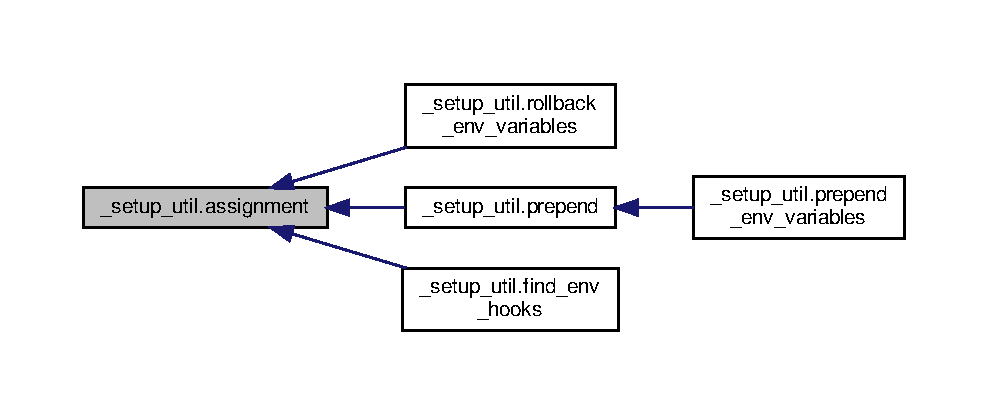
\includegraphics[width=350pt]{namespace__setup__util_ad56c24837fa4eddc63c03fbc7035628f_icgraph}
\end{center}
\end{figure}
\mbox{\Hypertarget{namespace__setup__util_abe8c95c4cfe8b1374dacd5f91d984353}\label{namespace__setup__util_abe8c95c4cfe8b1374dacd5f91d984353}} 
\index{\+\_\+setup\+\_\+util@{\+\_\+setup\+\_\+util}!comment@{comment}}
\index{comment@{comment}!\+\_\+setup\+\_\+util@{\+\_\+setup\+\_\+util}}
\subsubsection{\texorpdfstring{comment()}{comment()}}
{\footnotesize\ttfamily def \+\_\+setup\+\_\+util.\+comment (\begin{DoxyParamCaption}\item[{}]{msg }\end{DoxyParamCaption})}



Definition at line 182 of file \+\_\+setup\+\_\+util.\+py.

Here is the caller graph for this function\+:
\nopagebreak
\begin{figure}[H]
\begin{center}
\leavevmode
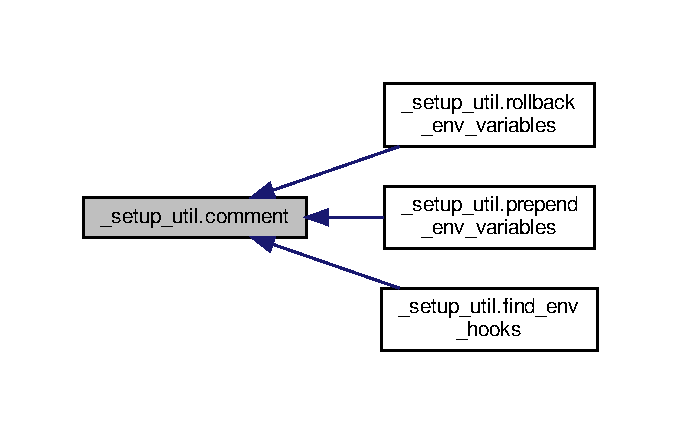
\includegraphics[width=327pt]{namespace__setup__util_abe8c95c4cfe8b1374dacd5f91d984353_icgraph}
\end{center}
\end{figure}
\mbox{\Hypertarget{namespace__setup__util_a73de35ca77f260af6691470342ab49ce}\label{namespace__setup__util_a73de35ca77f260af6691470342ab49ce}} 
\index{\+\_\+setup\+\_\+util@{\+\_\+setup\+\_\+util}!find\+\_\+env\+\_\+hooks@{find\+\_\+env\+\_\+hooks}}
\index{find\+\_\+env\+\_\+hooks@{find\+\_\+env\+\_\+hooks}!\+\_\+setup\+\_\+util@{\+\_\+setup\+\_\+util}}
\subsubsection{\texorpdfstring{find\+\_\+env\+\_\+hooks()}{find\_env\_hooks()}}
{\footnotesize\ttfamily def \+\_\+setup\+\_\+util.\+find\+\_\+env\+\_\+hooks (\begin{DoxyParamCaption}\item[{}]{environ,  }\item[{}]{cmake\+\_\+prefix\+\_\+path }\end{DoxyParamCaption})}

\begin{DoxyVerb}Generate shell code with found environment hooks
for the all workspaces.
\end{DoxyVerb}
 

Definition at line 198 of file \+\_\+setup\+\_\+util.\+py.

Here is the call graph for this function\+:
\nopagebreak
\begin{figure}[H]
\begin{center}
\leavevmode
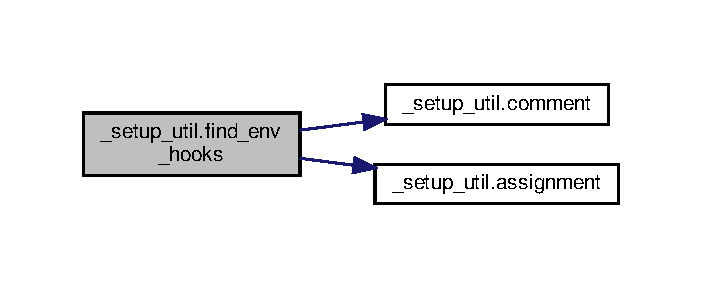
\includegraphics[width=337pt]{namespace__setup__util_a73de35ca77f260af6691470342ab49ce_cgraph}
\end{center}
\end{figure}
\mbox{\Hypertarget{namespace__setup__util_ae78d86b2c4279f5b8b1acaa146c35802}\label{namespace__setup__util_ae78d86b2c4279f5b8b1acaa146c35802}} 
\index{\+\_\+setup\+\_\+util@{\+\_\+setup\+\_\+util}!prepend@{prepend}}
\index{prepend@{prepend}!\+\_\+setup\+\_\+util@{\+\_\+setup\+\_\+util}}
\subsubsection{\texorpdfstring{prepend()}{prepend()}}
{\footnotesize\ttfamily def \+\_\+setup\+\_\+util.\+prepend (\begin{DoxyParamCaption}\item[{}]{environ,  }\item[{}]{key,  }\item[{}]{prefix }\end{DoxyParamCaption})}



Definition at line 189 of file \+\_\+setup\+\_\+util.\+py.

Here is the call graph for this function\+:
\nopagebreak
\begin{figure}[H]
\begin{center}
\leavevmode
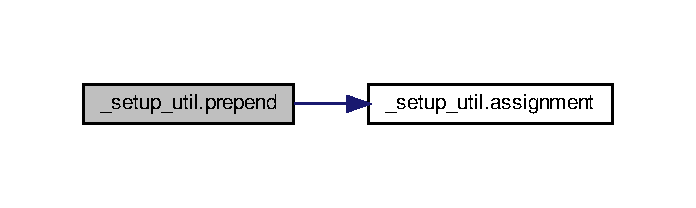
\includegraphics[width=334pt]{namespace__setup__util_ae78d86b2c4279f5b8b1acaa146c35802_cgraph}
\end{center}
\end{figure}
Here is the caller graph for this function\+:
\nopagebreak
\begin{figure}[H]
\begin{center}
\leavevmode
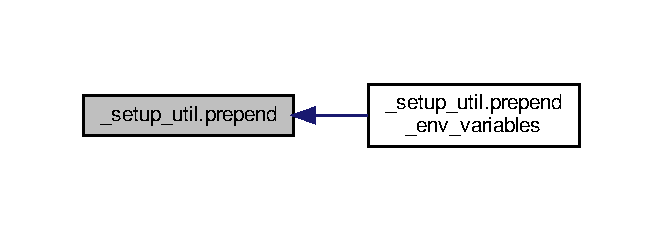
\includegraphics[width=318pt]{namespace__setup__util_ae78d86b2c4279f5b8b1acaa146c35802_icgraph}
\end{center}
\end{figure}
\mbox{\Hypertarget{namespace__setup__util_a832417d18b85bd1d276a87547e86f860}\label{namespace__setup__util_a832417d18b85bd1d276a87547e86f860}} 
\index{\+\_\+setup\+\_\+util@{\+\_\+setup\+\_\+util}!prepend\+\_\+env\+\_\+variables@{prepend\+\_\+env\+\_\+variables}}
\index{prepend\+\_\+env\+\_\+variables@{prepend\+\_\+env\+\_\+variables}!\+\_\+setup\+\_\+util@{\+\_\+setup\+\_\+util}}
\subsubsection{\texorpdfstring{prepend\+\_\+env\+\_\+variables()}{prepend\_env\_variables()}}
{\footnotesize\ttfamily def \+\_\+setup\+\_\+util.\+prepend\+\_\+env\+\_\+variables (\begin{DoxyParamCaption}\item[{}]{environ,  }\item[{}]{env\+\_\+var\+\_\+subfolders,  }\item[{}]{workspaces }\end{DoxyParamCaption})}

\begin{DoxyVerb}Generate shell code to prepend environment variables
for the all workspaces.
\end{DoxyVerb}
 

Definition at line 129 of file \+\_\+setup\+\_\+util.\+py.

Here is the call graph for this function\+:
\nopagebreak
\begin{figure}[H]
\begin{center}
\leavevmode
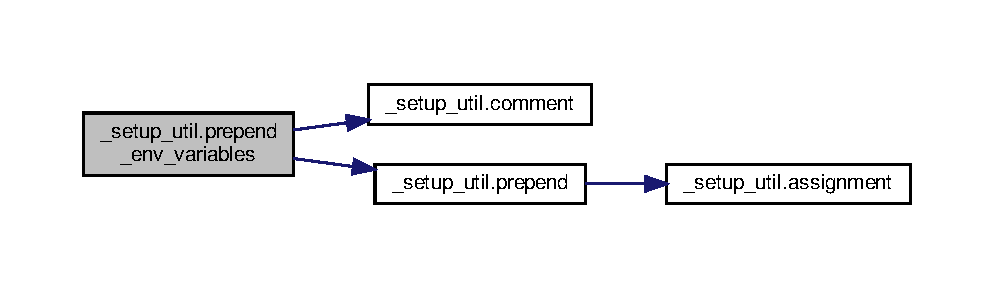
\includegraphics[width=350pt]{namespace__setup__util_a832417d18b85bd1d276a87547e86f860_cgraph}
\end{center}
\end{figure}
\mbox{\Hypertarget{namespace__setup__util_af3030db6102b5aa35cd354a2fb6cca03}\label{namespace__setup__util_af3030db6102b5aa35cd354a2fb6cca03}} 
\index{\+\_\+setup\+\_\+util@{\+\_\+setup\+\_\+util}!rollback\+\_\+env\+\_\+variables@{rollback\+\_\+env\+\_\+variables}}
\index{rollback\+\_\+env\+\_\+variables@{rollback\+\_\+env\+\_\+variables}!\+\_\+setup\+\_\+util@{\+\_\+setup\+\_\+util}}
\subsubsection{\texorpdfstring{rollback\+\_\+env\+\_\+variables()}{rollback\_env\_variables()}}
{\footnotesize\ttfamily def \+\_\+setup\+\_\+util.\+rollback\+\_\+env\+\_\+variables (\begin{DoxyParamCaption}\item[{}]{environ,  }\item[{}]{env\+\_\+var\+\_\+subfolders }\end{DoxyParamCaption})}

\begin{DoxyVerb}Generate shell code to reset environment variables
by unrolling modifications based on all workspaces in CMAKE_PREFIX_PATH.
This does not cover modifications performed by environment hooks.
\end{DoxyVerb}
 

Definition at line 62 of file \+\_\+setup\+\_\+util.\+py.

Here is the call graph for this function\+:
\nopagebreak
\begin{figure}[H]
\begin{center}
\leavevmode
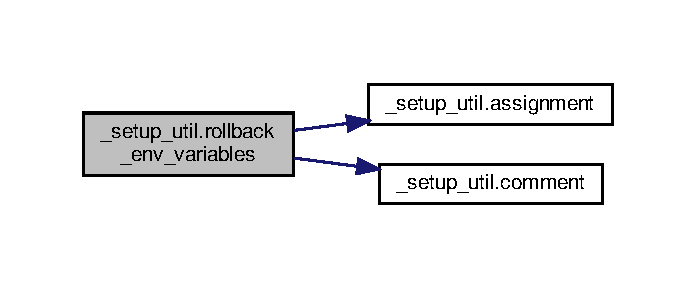
\includegraphics[width=334pt]{namespace__setup__util_af3030db6102b5aa35cd354a2fb6cca03_cgraph}
\end{center}
\end{figure}


\subsection{Variable Documentation}
\mbox{\Hypertarget{namespace__setup__util_a831491331b0650d492585147f04d6615}\label{namespace__setup__util_a831491331b0650d492585147f04d6615}} 
\index{\+\_\+setup\+\_\+util@{\+\_\+setup\+\_\+util}!args@{args}}
\index{args@{args}!\+\_\+setup\+\_\+util@{\+\_\+setup\+\_\+util}}
\subsubsection{\texorpdfstring{args}{args}}
{\footnotesize\ttfamily def \+\_\+setup\+\_\+util.\+args = \+\_\+parse\+\_\+arguments()}



Definition at line 260 of file \+\_\+setup\+\_\+util.\+py.

\mbox{\Hypertarget{namespace__setup__util_a83d25140acd7788bbcb95843fe38e639}\label{namespace__setup__util_a83d25140acd7788bbcb95843fe38e639}} 
\index{\+\_\+setup\+\_\+util@{\+\_\+setup\+\_\+util}!base\+\_\+path@{base\+\_\+path}}
\index{base\+\_\+path@{base\+\_\+path}!\+\_\+setup\+\_\+util@{\+\_\+setup\+\_\+util}}
\subsubsection{\texorpdfstring{base\+\_\+path}{base\_path}}
{\footnotesize\ttfamily \+\_\+setup\+\_\+util.\+base\+\_\+path = os.\+path.\+dirname(\+\_\+\+\_\+file\+\_\+\+\_\+)}



Definition at line 272 of file \+\_\+setup\+\_\+util.\+py.

\mbox{\Hypertarget{namespace__setup__util_a3fa0ca5a460a71a43cbc3d4954ab1f10}\label{namespace__setup__util_a3fa0ca5a460a71a43cbc3d4954ab1f10}} 
\index{\+\_\+setup\+\_\+util@{\+\_\+setup\+\_\+util}!C\+A\+T\+K\+I\+N\+\_\+\+M\+A\+R\+K\+E\+R\+\_\+\+F\+I\+LE@{C\+A\+T\+K\+I\+N\+\_\+\+M\+A\+R\+K\+E\+R\+\_\+\+F\+I\+LE}}
\index{C\+A\+T\+K\+I\+N\+\_\+\+M\+A\+R\+K\+E\+R\+\_\+\+F\+I\+LE@{C\+A\+T\+K\+I\+N\+\_\+\+M\+A\+R\+K\+E\+R\+\_\+\+F\+I\+LE}!\+\_\+setup\+\_\+util@{\+\_\+setup\+\_\+util}}
\subsubsection{\texorpdfstring{C\+A\+T\+K\+I\+N\+\_\+\+M\+A\+R\+K\+E\+R\+\_\+\+F\+I\+LE}{CATKIN\_MARKER\_FILE}}
{\footnotesize\ttfamily string \+\_\+setup\+\_\+util.\+C\+A\+T\+K\+I\+N\+\_\+\+M\+A\+R\+K\+E\+R\+\_\+\+F\+I\+LE = \textquotesingle{}.catkin\textquotesingle{}}



Definition at line 46 of file \+\_\+setup\+\_\+util.\+py.

\mbox{\Hypertarget{namespace__setup__util_a2a6756158bb4094ed7d259eb564d0578}\label{namespace__setup__util_a2a6756158bb4094ed7d259eb564d0578}} 
\index{\+\_\+setup\+\_\+util@{\+\_\+setup\+\_\+util}!C\+M\+A\+K\+E\+\_\+\+P\+R\+E\+F\+I\+X\+\_\+\+P\+A\+TH@{C\+M\+A\+K\+E\+\_\+\+P\+R\+E\+F\+I\+X\+\_\+\+P\+A\+TH}}
\index{C\+M\+A\+K\+E\+\_\+\+P\+R\+E\+F\+I\+X\+\_\+\+P\+A\+TH@{C\+M\+A\+K\+E\+\_\+\+P\+R\+E\+F\+I\+X\+\_\+\+P\+A\+TH}!\+\_\+setup\+\_\+util@{\+\_\+setup\+\_\+util}}
\subsubsection{\texorpdfstring{C\+M\+A\+K\+E\+\_\+\+P\+R\+E\+F\+I\+X\+\_\+\+P\+A\+TH}{CMAKE\_PREFIX\_PATH}}
{\footnotesize\ttfamily list \+\_\+setup\+\_\+util.\+C\+M\+A\+K\+E\+\_\+\+P\+R\+E\+F\+I\+X\+\_\+\+P\+A\+TH = \textquotesingle{}/home/jungwon/catkin\+\_\+ws/devel;/opt/ros/melodic\textquotesingle{}.split(\textquotesingle{};\textquotesingle{})}



Definition at line 267 of file \+\_\+setup\+\_\+util.\+py.

\mbox{\Hypertarget{namespace__setup__util_acdce690b925de33d6249bbbfa1109d61}\label{namespace__setup__util_acdce690b925de33d6249bbbfa1109d61}} 
\index{\+\_\+setup\+\_\+util@{\+\_\+setup\+\_\+util}!e@{e}}
\index{e@{e}!\+\_\+setup\+\_\+util@{\+\_\+setup\+\_\+util}}
\subsubsection{\texorpdfstring{e}{e}}
{\footnotesize\ttfamily \+\_\+setup\+\_\+util.\+e}



Definition at line 262 of file \+\_\+setup\+\_\+util.\+py.

\mbox{\Hypertarget{namespace__setup__util_aa31804f1be8660156ce9394b33c68dc4}\label{namespace__setup__util_aa31804f1be8660156ce9394b33c68dc4}} 
\index{\+\_\+setup\+\_\+util@{\+\_\+setup\+\_\+util}!E\+N\+V\+\_\+\+V\+A\+R\+\_\+\+S\+U\+B\+F\+O\+L\+D\+E\+RS@{E\+N\+V\+\_\+\+V\+A\+R\+\_\+\+S\+U\+B\+F\+O\+L\+D\+E\+RS}}
\index{E\+N\+V\+\_\+\+V\+A\+R\+\_\+\+S\+U\+B\+F\+O\+L\+D\+E\+RS@{E\+N\+V\+\_\+\+V\+A\+R\+\_\+\+S\+U\+B\+F\+O\+L\+D\+E\+RS}!\+\_\+setup\+\_\+util@{\+\_\+setup\+\_\+util}}
\subsubsection{\texorpdfstring{E\+N\+V\+\_\+\+V\+A\+R\+\_\+\+S\+U\+B\+F\+O\+L\+D\+E\+RS}{ENV\_VAR\_SUBFOLDERS}}
{\footnotesize\ttfamily dictionary \+\_\+setup\+\_\+util.\+E\+N\+V\+\_\+\+V\+A\+R\+\_\+\+S\+U\+B\+F\+O\+L\+D\+E\+RS}

{\bfseries Initial value\+:}
\begin{DoxyCode}
1 =  \{
2     \textcolor{stringliteral}{'CMAKE\_PREFIX\_PATH'}: \textcolor{stringliteral}{''},
3     \textcolor{stringliteral}{'LD\_LIBRARY\_PATH'} \textcolor{keywordflow}{if} \textcolor{keywordflow}{not} IS\_DARWIN \textcolor{keywordflow}{else} \textcolor{stringliteral}{'DYLD\_LIBRARY\_PATH'}: [\textcolor{stringliteral}{'lib'}, os.path.join(\textcolor{stringliteral}{'lib'}, \textcolor{stringliteral}{'
      x86\_64-linux-gnu'})],
4     \textcolor{stringliteral}{'PATH'}: \textcolor{stringliteral}{'bin'},
5     \textcolor{stringliteral}{'PKG\_CONFIG\_PATH'}: [os.path.join(\textcolor{stringliteral}{'lib'}, \textcolor{stringliteral}{'pkgconfig'}), os.path.join(\textcolor{stringliteral}{'lib'}, \textcolor{stringliteral}{'x86\_64-linux-gnu'}, \textcolor{stringliteral}{'
      pkgconfig'})],
6     \textcolor{stringliteral}{'PYTHONPATH'}: \textcolor{stringliteral}{'lib/python2.7/dist-packages'},
7 \}
\end{DoxyCode}


Definition at line 53 of file \+\_\+setup\+\_\+util.\+py.

\mbox{\Hypertarget{namespace__setup__util_a9a935bdd9ee1aa0327161025bb18c136}\label{namespace__setup__util_a9a935bdd9ee1aa0327161025bb18c136}} 
\index{\+\_\+setup\+\_\+util@{\+\_\+setup\+\_\+util}!environ@{environ}}
\index{environ@{environ}!\+\_\+setup\+\_\+util@{\+\_\+setup\+\_\+util}}
\subsubsection{\texorpdfstring{environ}{environ}}
{\footnotesize\ttfamily \+\_\+setup\+\_\+util.\+environ = dict(os.\+environ)}



Definition at line 282 of file \+\_\+setup\+\_\+util.\+py.

\mbox{\Hypertarget{namespace__setup__util_aea63a1b32cc79bc3d872ab7cb30dd07e}\label{namespace__setup__util_aea63a1b32cc79bc3d872ab7cb30dd07e}} 
\index{\+\_\+setup\+\_\+util@{\+\_\+setup\+\_\+util}!file@{file}}
\index{file@{file}!\+\_\+setup\+\_\+util@{\+\_\+setup\+\_\+util}}
\subsubsection{\texorpdfstring{file}{file}}
{\footnotesize\ttfamily \+\_\+setup\+\_\+util.\+file}



Definition at line 262 of file \+\_\+setup\+\_\+util.\+py.

\mbox{\Hypertarget{namespace__setup__util_aecbb100ce6f94bb3c7e16d58fde05f96}\label{namespace__setup__util_aecbb100ce6f94bb3c7e16d58fde05f96}} 
\index{\+\_\+setup\+\_\+util@{\+\_\+setup\+\_\+util}!I\+S\+\_\+\+D\+A\+R\+W\+IN@{I\+S\+\_\+\+D\+A\+R\+W\+IN}}
\index{I\+S\+\_\+\+D\+A\+R\+W\+IN@{I\+S\+\_\+\+D\+A\+R\+W\+IN}!\+\_\+setup\+\_\+util@{\+\_\+setup\+\_\+util}}
\subsubsection{\texorpdfstring{I\+S\+\_\+\+D\+A\+R\+W\+IN}{IS\_DARWIN}}
{\footnotesize\ttfamily tuple \+\_\+setup\+\_\+util.\+I\+S\+\_\+\+D\+A\+R\+W\+IN = (\hyperlink{namespace__setup__util_ae9fca6a80a6923f4580be72f68fee325}{system} == \textquotesingle{}Darwin\textquotesingle{})}



Definition at line 49 of file \+\_\+setup\+\_\+util.\+py.

\mbox{\Hypertarget{namespace__setup__util_a6fe69c2dbd92959b6651a28cbb846e6e}\label{namespace__setup__util_a6fe69c2dbd92959b6651a28cbb846e6e}} 
\index{\+\_\+setup\+\_\+util@{\+\_\+setup\+\_\+util}!I\+S\+\_\+\+W\+I\+N\+D\+O\+WS@{I\+S\+\_\+\+W\+I\+N\+D\+O\+WS}}
\index{I\+S\+\_\+\+W\+I\+N\+D\+O\+WS@{I\+S\+\_\+\+W\+I\+N\+D\+O\+WS}!\+\_\+setup\+\_\+util@{\+\_\+setup\+\_\+util}}
\subsubsection{\texorpdfstring{I\+S\+\_\+\+W\+I\+N\+D\+O\+WS}{IS\_WINDOWS}}
{\footnotesize\ttfamily tuple \+\_\+setup\+\_\+util.\+I\+S\+\_\+\+W\+I\+N\+D\+O\+WS = (\hyperlink{namespace__setup__util_ae9fca6a80a6923f4580be72f68fee325}{system} == \textquotesingle{}Windows\textquotesingle{})}



Definition at line 50 of file \+\_\+setup\+\_\+util.\+py.

\mbox{\Hypertarget{namespace__setup__util_a8618d8be5f729d4c9696daa5e083a001}\label{namespace__setup__util_a8618d8be5f729d4c9696daa5e083a001}} 
\index{\+\_\+setup\+\_\+util@{\+\_\+setup\+\_\+util}!lines@{lines}}
\index{lines@{lines}!\+\_\+setup\+\_\+util@{\+\_\+setup\+\_\+util}}
\subsubsection{\texorpdfstring{lines}{lines}}
{\footnotesize\ttfamily list \+\_\+setup\+\_\+util.\+lines = \mbox{[}$\,$\mbox{]}}



Definition at line 283 of file \+\_\+setup\+\_\+util.\+py.

\mbox{\Hypertarget{namespace__setup__util_ae9fca6a80a6923f4580be72f68fee325}\label{namespace__setup__util_ae9fca6a80a6923f4580be72f68fee325}} 
\index{\+\_\+setup\+\_\+util@{\+\_\+setup\+\_\+util}!system@{system}}
\index{system@{system}!\+\_\+setup\+\_\+util@{\+\_\+setup\+\_\+util}}
\subsubsection{\texorpdfstring{system}{system}}
{\footnotesize\ttfamily \+\_\+setup\+\_\+util.\+system = platform.\+system()}



Definition at line 48 of file \+\_\+setup\+\_\+util.\+py.


\hypertarget{namespacegenerate__cached__setup}{}\section{generate\+\_\+cached\+\_\+setup Namespace Reference}
\label{namespacegenerate__cached__setup}\index{generate\+\_\+cached\+\_\+setup@{generate\+\_\+cached\+\_\+setup}}
\subsection*{Variables}
\begin{DoxyCompactItemize}
\item 
\hyperlink{namespacegenerate__cached__setup_a72579fd01529a79bab20d99291889d3f}{python\+\_\+path} = os.\+path.\+join(workspace, \textquotesingle{}lib/python2.\+7/dist-\/packages\textquotesingle{})
\item 
\hyperlink{namespacegenerate__cached__setup_a52601295006f2366a311c4453d8f2f2e}{code} = generate\+\_\+environment\+\_\+script(\textquotesingle{}/home/jungwon/catkin\+\_\+ws/src/atypical\+\_\+planning/cmake-\/build-\/debug/devel/env.\+sh\textquotesingle{})
\item 
string \hyperlink{namespacegenerate__cached__setup_a0265aee5075ee1eb701ff69c98ad6793}{output\+\_\+filename} = \textquotesingle{}/home/jungwon/catkin\+\_\+ws/src/atypical\+\_\+planning/cmake-\/build-\/debug/catkin\+\_\+generated/setup\+\_\+cached.\+sh\textquotesingle{}
\item 
\hyperlink{namespacegenerate__cached__setup_a10081e5abedae9bd46dd91202096e789}{mode} = os.\+stat(\hyperlink{namespacegenerate__cached__setup_a0265aee5075ee1eb701ff69c98ad6793}{output\+\_\+filename}).st\+\_\+mode
\end{DoxyCompactItemize}


\subsection{Variable Documentation}
\mbox{\Hypertarget{namespacegenerate__cached__setup_a52601295006f2366a311c4453d8f2f2e}\label{namespacegenerate__cached__setup_a52601295006f2366a311c4453d8f2f2e}} 
\index{generate\+\_\+cached\+\_\+setup@{generate\+\_\+cached\+\_\+setup}!code@{code}}
\index{code@{code}!generate\+\_\+cached\+\_\+setup@{generate\+\_\+cached\+\_\+setup}}
\subsubsection{\texorpdfstring{code}{code}}
{\footnotesize\ttfamily generate\+\_\+cached\+\_\+setup.\+code = generate\+\_\+environment\+\_\+script(\textquotesingle{}/home/jungwon/catkin\+\_\+ws/src/atypical\+\_\+planning/cmake-\/build-\/debug/devel/env.\+sh\textquotesingle{})}



Definition at line 22 of file generate\+\_\+cached\+\_\+setup.\+py.

\mbox{\Hypertarget{namespacegenerate__cached__setup_a10081e5abedae9bd46dd91202096e789}\label{namespacegenerate__cached__setup_a10081e5abedae9bd46dd91202096e789}} 
\index{generate\+\_\+cached\+\_\+setup@{generate\+\_\+cached\+\_\+setup}!mode@{mode}}
\index{mode@{mode}!generate\+\_\+cached\+\_\+setup@{generate\+\_\+cached\+\_\+setup}}
\subsubsection{\texorpdfstring{mode}{mode}}
{\footnotesize\ttfamily generate\+\_\+cached\+\_\+setup.\+mode = os.\+stat(\hyperlink{namespacegenerate__cached__setup_a0265aee5075ee1eb701ff69c98ad6793}{output\+\_\+filename}).st\+\_\+mode}



Definition at line 29 of file generate\+\_\+cached\+\_\+setup.\+py.

\mbox{\Hypertarget{namespacegenerate__cached__setup_a0265aee5075ee1eb701ff69c98ad6793}\label{namespacegenerate__cached__setup_a0265aee5075ee1eb701ff69c98ad6793}} 
\index{generate\+\_\+cached\+\_\+setup@{generate\+\_\+cached\+\_\+setup}!output\+\_\+filename@{output\+\_\+filename}}
\index{output\+\_\+filename@{output\+\_\+filename}!generate\+\_\+cached\+\_\+setup@{generate\+\_\+cached\+\_\+setup}}
\subsubsection{\texorpdfstring{output\+\_\+filename}{output\_filename}}
{\footnotesize\ttfamily string generate\+\_\+cached\+\_\+setup.\+output\+\_\+filename = \textquotesingle{}/home/jungwon/catkin\+\_\+ws/src/atypical\+\_\+planning/cmake-\/build-\/debug/catkin\+\_\+generated/setup\+\_\+cached.\+sh\textquotesingle{}}



Definition at line 24 of file generate\+\_\+cached\+\_\+setup.\+py.

\mbox{\Hypertarget{namespacegenerate__cached__setup_a72579fd01529a79bab20d99291889d3f}\label{namespacegenerate__cached__setup_a72579fd01529a79bab20d99291889d3f}} 
\index{generate\+\_\+cached\+\_\+setup@{generate\+\_\+cached\+\_\+setup}!python\+\_\+path@{python\+\_\+path}}
\index{python\+\_\+path@{python\+\_\+path}!generate\+\_\+cached\+\_\+setup@{generate\+\_\+cached\+\_\+setup}}
\subsubsection{\texorpdfstring{python\+\_\+path}{python\_path}}
{\footnotesize\ttfamily generate\+\_\+cached\+\_\+setup.\+python\+\_\+path = os.\+path.\+join(workspace, \textquotesingle{}lib/python2.\+7/dist-\/packages\textquotesingle{})}



Definition at line 16 of file generate\+\_\+cached\+\_\+setup.\+py.


\hypertarget{namespacelib_corridor_gen}{}\section{lib\+Corridor\+Gen Namespace Reference}
\label{namespacelib_corridor_gen}\index{lib\+Corridor\+Gen@{lib\+Corridor\+Gen}}
\subsection*{Classes}
\begin{DoxyCompactItemize}
\item 
class \hyperlink{classlib_corridor_gen_1_1_corridor}{Corridor}
\item 
class \hyperlink{classlib_corridor_gen_1_1_e_c_b_s_planner}{E\+C\+B\+S\+Planner}
\item 
class \hyperlink{classlib_corridor_gen_1_1_init_traj_planner}{Init\+Traj\+Planner}
\item 
class \hyperlink{classlib_corridor_gen_1_1_param}{Param}
\item 
class \hyperlink{classlib_corridor_gen_1_1_result_publisher}{Result\+Publisher}
\item 
class \hyperlink{classlib_corridor_gen_1_1_wrapper}{Wrapper}
\end{DoxyCompactItemize}

\hypertarget{namespacelib_multi_robot_planning}{}\section{lib\+Multi\+Robot\+Planning Namespace Reference}
\label{namespacelib_multi_robot_planning}\index{lib\+Multi\+Robot\+Planning@{lib\+Multi\+Robot\+Planning}}
\subsection*{Classes}
\begin{DoxyCompactItemize}
\item 
class \hyperlink{classlib_multi_robot_planning_1_1_a_star}{A\+Star}
\begin{DoxyCompactList}\small\item\em A$\ast$ Algorithm to find the shortest path. \end{DoxyCompactList}\item 
class \hyperlink{classlib_multi_robot_planning_1_1_a_star_epsilon}{A\+Star\+Epsilon}
\begin{DoxyCompactList}\small\item\em A$\ast$\+\_\+epsilon Algorithm to find the shortest path with a given suboptimality bound (also known as focal search) \end{DoxyCompactList}\item 
class \hyperlink{classlib_multi_robot_planning_1_1_c_b_s}{C\+BS}
\begin{DoxyCompactList}\small\item\em Conflict-\/\+Based-\/\+Search (\hyperlink{classlib_multi_robot_planning_1_1_c_b_s}{C\+BS}) algorithm to solve the Multi-\/\+Agent Path-\/\+Finding (M\+A\+PF) problem. \end{DoxyCompactList}\item 
struct \hyperlink{structlib_multi_robot_planning_1_1_conflict}{Conflict}
\item 
struct \hyperlink{structlib_multi_robot_planning_1_1_constraints}{Constraints}
\item 
class \hyperlink{classlib_multi_robot_planning_1_1_e_c_b_s}{E\+C\+BS}
\begin{DoxyCompactList}\small\item\em Enhanced Conflict-\/\+Based-\/\+Search (\hyperlink{classlib_multi_robot_planning_1_1_e_c_b_s}{E\+C\+BS}) algorithm to solve the Multi-\/\+Agent Path-\/\+Finding (M\+A\+PF) problem within a given suboptimality bound. \end{DoxyCompactList}\item 
struct \hyperlink{structlib_multi_robot_planning_1_1_edge_constraint}{Edge\+Constraint}
\item 
class \hyperlink{classlib_multi_robot_planning_1_1_environment}{Environment}
\item 
struct \hyperlink{structlib_multi_robot_planning_1_1_location}{Location}
\item 
struct \hyperlink{structlib_multi_robot_planning_1_1_neighbor}{Neighbor}
\begin{DoxyCompactList}\small\item\em Represents state transations. \end{DoxyCompactList}\item 
struct \hyperlink{structlib_multi_robot_planning_1_1_plan_result}{Plan\+Result}
\begin{DoxyCompactList}\small\item\em Represents the path for an agent. \end{DoxyCompactList}\item 
struct \hyperlink{structlib_multi_robot_planning_1_1_state}{State}
\item 
struct \hyperlink{structlib_multi_robot_planning_1_1_vertex_constraint}{Vertex\+Constraint}
\end{DoxyCompactItemize}
\subsection*{Enumerations}
\begin{DoxyCompactItemize}
\item 
enum \hyperlink{namespacelib_multi_robot_planning_aba73fb71693f86a324adfa0e41e1053d}{Action} \{ \newline
\hyperlink{namespacelib_multi_robot_planning_aba73fb71693f86a324adfa0e41e1053da258f49887ef8d14ac268c92b02503aaa}{Action\+::\+Up}, 
\hyperlink{namespacelib_multi_robot_planning_aba73fb71693f86a324adfa0e41e1053da08a38277b0309070706f6652eeae9a53}{Action\+::\+Down}, 
\hyperlink{namespacelib_multi_robot_planning_aba73fb71693f86a324adfa0e41e1053da945d5e233cf7d6240f6b783b36a374ff}{Action\+::\+Left}, 
\hyperlink{namespacelib_multi_robot_planning_aba73fb71693f86a324adfa0e41e1053da92b09c7c48c520c3c55e497875da437c}{Action\+::\+Right}, 
\newline
\hyperlink{namespacelib_multi_robot_planning_aba73fb71693f86a324adfa0e41e1053daa4ffdcf0dc1f31b9acaf295d75b51d00}{Action\+::\+Top}, 
\hyperlink{namespacelib_multi_robot_planning_aba73fb71693f86a324adfa0e41e1053da2ad9d63b69c4a10a5cc9cad923133bc4}{Action\+::\+Bottom}, 
\hyperlink{namespacelib_multi_robot_planning_aba73fb71693f86a324adfa0e41e1053da0f68101772bd5397ef8eb1b632798652}{Action\+::\+Wait}
 \}
\end{DoxyCompactItemize}
\subsection*{Functions}
\begin{DoxyCompactItemize}
\item 
std\+::ostream \& \hyperlink{namespacelib_multi_robot_planning_ac64bacf3115f1341bd7ce739c119f00a}{operator$<$$<$} (std\+::ostream \&os, const \hyperlink{namespacelib_multi_robot_planning_aba73fb71693f86a324adfa0e41e1053d}{Action} \&a)
\end{DoxyCompactItemize}


\subsection{Enumeration Type Documentation}
\mbox{\Hypertarget{namespacelib_multi_robot_planning_aba73fb71693f86a324adfa0e41e1053d}\label{namespacelib_multi_robot_planning_aba73fb71693f86a324adfa0e41e1053d}} 
\index{lib\+Multi\+Robot\+Planning@{lib\+Multi\+Robot\+Planning}!Action@{Action}}
\index{Action@{Action}!lib\+Multi\+Robot\+Planning@{lib\+Multi\+Robot\+Planning}}
\subsubsection{\texorpdfstring{Action}{Action}}
{\footnotesize\ttfamily enum \hyperlink{namespacelib_multi_robot_planning_aba73fb71693f86a324adfa0e41e1053d}{lib\+Multi\+Robot\+Planning\+::\+Action}\hspace{0.3cm}{\ttfamily [strong]}}

\begin{DoxyEnumFields}{Enumerator}
\raisebox{\heightof{T}}[0pt][0pt]{\index{Up@{Up}!lib\+Multi\+Robot\+Planning@{lib\+Multi\+Robot\+Planning}}\index{lib\+Multi\+Robot\+Planning@{lib\+Multi\+Robot\+Planning}!Up@{Up}}}\mbox{\Hypertarget{namespacelib_multi_robot_planning_aba73fb71693f86a324adfa0e41e1053da258f49887ef8d14ac268c92b02503aaa}\label{namespacelib_multi_robot_planning_aba73fb71693f86a324adfa0e41e1053da258f49887ef8d14ac268c92b02503aaa}} 
Up&\\
\hline

\raisebox{\heightof{T}}[0pt][0pt]{\index{Down@{Down}!lib\+Multi\+Robot\+Planning@{lib\+Multi\+Robot\+Planning}}\index{lib\+Multi\+Robot\+Planning@{lib\+Multi\+Robot\+Planning}!Down@{Down}}}\mbox{\Hypertarget{namespacelib_multi_robot_planning_aba73fb71693f86a324adfa0e41e1053da08a38277b0309070706f6652eeae9a53}\label{namespacelib_multi_robot_planning_aba73fb71693f86a324adfa0e41e1053da08a38277b0309070706f6652eeae9a53}} 
Down&\\
\hline

\raisebox{\heightof{T}}[0pt][0pt]{\index{Left@{Left}!lib\+Multi\+Robot\+Planning@{lib\+Multi\+Robot\+Planning}}\index{lib\+Multi\+Robot\+Planning@{lib\+Multi\+Robot\+Planning}!Left@{Left}}}\mbox{\Hypertarget{namespacelib_multi_robot_planning_aba73fb71693f86a324adfa0e41e1053da945d5e233cf7d6240f6b783b36a374ff}\label{namespacelib_multi_robot_planning_aba73fb71693f86a324adfa0e41e1053da945d5e233cf7d6240f6b783b36a374ff}} 
Left&\\
\hline

\raisebox{\heightof{T}}[0pt][0pt]{\index{Right@{Right}!lib\+Multi\+Robot\+Planning@{lib\+Multi\+Robot\+Planning}}\index{lib\+Multi\+Robot\+Planning@{lib\+Multi\+Robot\+Planning}!Right@{Right}}}\mbox{\Hypertarget{namespacelib_multi_robot_planning_aba73fb71693f86a324adfa0e41e1053da92b09c7c48c520c3c55e497875da437c}\label{namespacelib_multi_robot_planning_aba73fb71693f86a324adfa0e41e1053da92b09c7c48c520c3c55e497875da437c}} 
Right&\\
\hline

\raisebox{\heightof{T}}[0pt][0pt]{\index{Top@{Top}!lib\+Multi\+Robot\+Planning@{lib\+Multi\+Robot\+Planning}}\index{lib\+Multi\+Robot\+Planning@{lib\+Multi\+Robot\+Planning}!Top@{Top}}}\mbox{\Hypertarget{namespacelib_multi_robot_planning_aba73fb71693f86a324adfa0e41e1053daa4ffdcf0dc1f31b9acaf295d75b51d00}\label{namespacelib_multi_robot_planning_aba73fb71693f86a324adfa0e41e1053daa4ffdcf0dc1f31b9acaf295d75b51d00}} 
Top&\\
\hline

\raisebox{\heightof{T}}[0pt][0pt]{\index{Bottom@{Bottom}!lib\+Multi\+Robot\+Planning@{lib\+Multi\+Robot\+Planning}}\index{lib\+Multi\+Robot\+Planning@{lib\+Multi\+Robot\+Planning}!Bottom@{Bottom}}}\mbox{\Hypertarget{namespacelib_multi_robot_planning_aba73fb71693f86a324adfa0e41e1053da2ad9d63b69c4a10a5cc9cad923133bc4}\label{namespacelib_multi_robot_planning_aba73fb71693f86a324adfa0e41e1053da2ad9d63b69c4a10a5cc9cad923133bc4}} 
Bottom&\\
\hline

\raisebox{\heightof{T}}[0pt][0pt]{\index{Wait@{Wait}!lib\+Multi\+Robot\+Planning@{lib\+Multi\+Robot\+Planning}}\index{lib\+Multi\+Robot\+Planning@{lib\+Multi\+Robot\+Planning}!Wait@{Wait}}}\mbox{\Hypertarget{namespacelib_multi_robot_planning_aba73fb71693f86a324adfa0e41e1053da0f68101772bd5397ef8eb1b632798652}\label{namespacelib_multi_robot_planning_aba73fb71693f86a324adfa0e41e1053da0f68101772bd5397ef8eb1b632798652}} 
Wait&\\
\hline

\end{DoxyEnumFields}


Definition at line 53 of file environment.\+hpp.



\subsection{Function Documentation}
\mbox{\Hypertarget{namespacelib_multi_robot_planning_ac64bacf3115f1341bd7ce739c119f00a}\label{namespacelib_multi_robot_planning_ac64bacf3115f1341bd7ce739c119f00a}} 
\index{lib\+Multi\+Robot\+Planning@{lib\+Multi\+Robot\+Planning}!operator$<$$<$@{operator$<$$<$}}
\index{operator$<$$<$@{operator$<$$<$}!lib\+Multi\+Robot\+Planning@{lib\+Multi\+Robot\+Planning}}
\subsubsection{\texorpdfstring{operator$<$$<$()}{operator<<()}}
{\footnotesize\ttfamily std\+::ostream\& lib\+Multi\+Robot\+Planning\+::operator$<$$<$ (\begin{DoxyParamCaption}\item[{std\+::ostream \&}]{os,  }\item[{const \hyperlink{namespacelib_multi_robot_planning_aba73fb71693f86a324adfa0e41e1053d}{Action} \&}]{a }\end{DoxyParamCaption})}



Definition at line 63 of file environment.\+hpp.

Here is the caller graph for this function\+:
\nopagebreak
\begin{figure}[H]
\begin{center}
\leavevmode
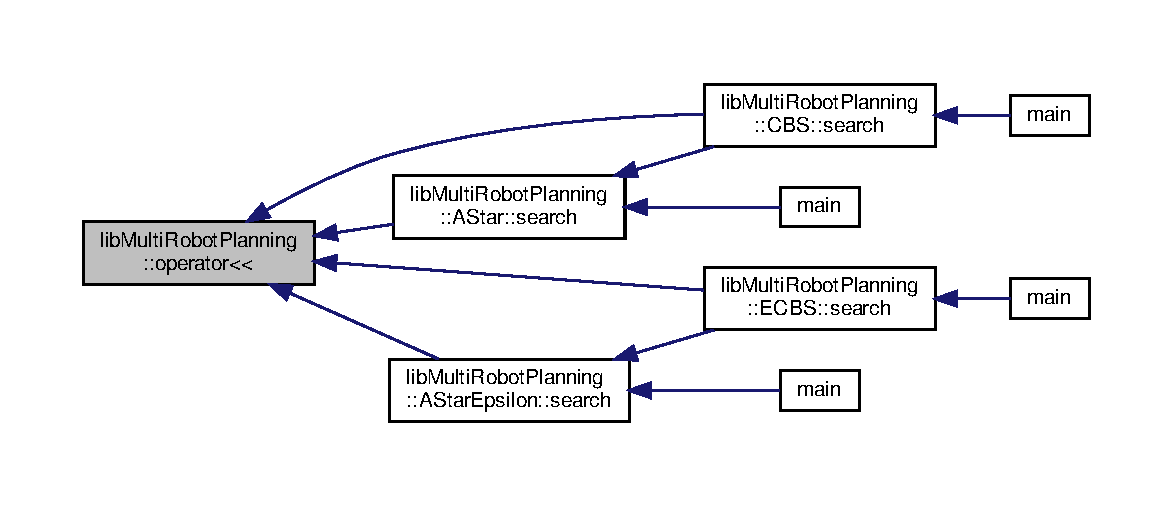
\includegraphics[width=350pt]{namespacelib_multi_robot_planning_ac64bacf3115f1341bd7ce739c119f00a_icgraph}
\end{center}
\end{figure}

\hypertarget{namespacepkg}{}\section{pkg Namespace Reference}
\label{namespacepkg}\index{pkg@{pkg}}
\subsection*{Variables}
\begin{DoxyCompactItemize}
\item 
string \hyperlink{namespacepkg_ae26c7a5a06b7d738f4d210ca449e6bee}{C\+A\+T\+K\+I\+N\+\_\+\+P\+A\+C\+K\+A\+G\+E\+\_\+\+P\+R\+E\+F\+IX} = \char`\"{}\char`\"{}
\item 
string \hyperlink{namespacepkg_a2760bf8266ff58da440f65ee91b203ab}{P\+R\+O\+J\+E\+C\+T\+\_\+\+P\+K\+G\+\_\+\+C\+O\+N\+F\+I\+G\+\_\+\+I\+N\+C\+L\+U\+D\+E\+\_\+\+D\+I\+RS} = \char`\"{}\char`\"{} else \mbox{[}$\,$\mbox{]}
\item 
string \hyperlink{namespacepkg_a17c18447fad253ee1c0d76deec88028c}{P\+R\+O\+J\+E\+C\+T\+\_\+\+C\+A\+T\+K\+I\+N\+\_\+\+D\+E\+P\+E\+N\+DS} = \char`\"{}roscpp;roslib\char`\"{}.replace(\textquotesingle{};\textquotesingle{}, \textquotesingle{} \textquotesingle{})
\item 
string \hyperlink{namespacepkg_a433e30cecb4a0123a7c4b384d168e336}{P\+K\+G\+\_\+\+C\+O\+N\+F\+I\+G\+\_\+\+L\+I\+B\+R\+A\+R\+I\+E\+S\+\_\+\+W\+I\+T\+H\+\_\+\+P\+R\+E\+F\+IX} = \char`\"{}\char`\"{} else \mbox{[}$\,$\mbox{]}
\item 
string \hyperlink{namespacepkg_a7dfbe99257c26f5e4a3a5483995d9ddc}{P\+R\+O\+J\+E\+C\+T\+\_\+\+N\+A\+ME} = \char`\"{}atypical\+\_\+planning\char`\"{}
\item 
string \hyperlink{namespacepkg_a3f0f1b4bc03c596525e025539ca4332f}{P\+R\+O\+J\+E\+C\+T\+\_\+\+S\+P\+A\+C\+E\+\_\+\+D\+IR} = \char`\"{}/home/jungwon/catkin\+\_\+ws/src/atypical\+\_\+planning/cmake-\/build-\/debug/devel\char`\"{}
\item 
string \hyperlink{namespacepkg_ab1037914b9286bb61855131c06149648}{P\+R\+O\+J\+E\+C\+T\+\_\+\+V\+E\+R\+S\+I\+ON} = \char`\"{}0.\+0.\+0\char`\"{}
\end{DoxyCompactItemize}


\subsection{Variable Documentation}
\mbox{\Hypertarget{namespacepkg_ae26c7a5a06b7d738f4d210ca449e6bee}\label{namespacepkg_ae26c7a5a06b7d738f4d210ca449e6bee}} 
\index{pkg@{pkg}!C\+A\+T\+K\+I\+N\+\_\+\+P\+A\+C\+K\+A\+G\+E\+\_\+\+P\+R\+E\+F\+IX@{C\+A\+T\+K\+I\+N\+\_\+\+P\+A\+C\+K\+A\+G\+E\+\_\+\+P\+R\+E\+F\+IX}}
\index{C\+A\+T\+K\+I\+N\+\_\+\+P\+A\+C\+K\+A\+G\+E\+\_\+\+P\+R\+E\+F\+IX@{C\+A\+T\+K\+I\+N\+\_\+\+P\+A\+C\+K\+A\+G\+E\+\_\+\+P\+R\+E\+F\+IX}!pkg@{pkg}}
\subsubsection{\texorpdfstring{C\+A\+T\+K\+I\+N\+\_\+\+P\+A\+C\+K\+A\+G\+E\+\_\+\+P\+R\+E\+F\+IX}{CATKIN\_PACKAGE\_PREFIX}}
{\footnotesize\ttfamily string pkg.\+C\+A\+T\+K\+I\+N\+\_\+\+P\+A\+C\+K\+A\+G\+E\+\_\+\+P\+R\+E\+F\+IX = \char`\"{}\char`\"{}}



Definition at line 2 of file pkg.\+develspace.\+context.\+pc.\+py.

\mbox{\Hypertarget{namespacepkg_a433e30cecb4a0123a7c4b384d168e336}\label{namespacepkg_a433e30cecb4a0123a7c4b384d168e336}} 
\index{pkg@{pkg}!P\+K\+G\+\_\+\+C\+O\+N\+F\+I\+G\+\_\+\+L\+I\+B\+R\+A\+R\+I\+E\+S\+\_\+\+W\+I\+T\+H\+\_\+\+P\+R\+E\+F\+IX@{P\+K\+G\+\_\+\+C\+O\+N\+F\+I\+G\+\_\+\+L\+I\+B\+R\+A\+R\+I\+E\+S\+\_\+\+W\+I\+T\+H\+\_\+\+P\+R\+E\+F\+IX}}
\index{P\+K\+G\+\_\+\+C\+O\+N\+F\+I\+G\+\_\+\+L\+I\+B\+R\+A\+R\+I\+E\+S\+\_\+\+W\+I\+T\+H\+\_\+\+P\+R\+E\+F\+IX@{P\+K\+G\+\_\+\+C\+O\+N\+F\+I\+G\+\_\+\+L\+I\+B\+R\+A\+R\+I\+E\+S\+\_\+\+W\+I\+T\+H\+\_\+\+P\+R\+E\+F\+IX}!pkg@{pkg}}
\subsubsection{\texorpdfstring{P\+K\+G\+\_\+\+C\+O\+N\+F\+I\+G\+\_\+\+L\+I\+B\+R\+A\+R\+I\+E\+S\+\_\+\+W\+I\+T\+H\+\_\+\+P\+R\+E\+F\+IX}{PKG\_CONFIG\_LIBRARIES\_WITH\_PREFIX}}
{\footnotesize\ttfamily string pkg.\+P\+K\+G\+\_\+\+C\+O\+N\+F\+I\+G\+\_\+\+L\+I\+B\+R\+A\+R\+I\+E\+S\+\_\+\+W\+I\+T\+H\+\_\+\+P\+R\+E\+F\+IX = \char`\"{}\char`\"{} else \mbox{[}$\,$\mbox{]}}



Definition at line 5 of file pkg.\+develspace.\+context.\+pc.\+py.

\mbox{\Hypertarget{namespacepkg_a17c18447fad253ee1c0d76deec88028c}\label{namespacepkg_a17c18447fad253ee1c0d76deec88028c}} 
\index{pkg@{pkg}!P\+R\+O\+J\+E\+C\+T\+\_\+\+C\+A\+T\+K\+I\+N\+\_\+\+D\+E\+P\+E\+N\+DS@{P\+R\+O\+J\+E\+C\+T\+\_\+\+C\+A\+T\+K\+I\+N\+\_\+\+D\+E\+P\+E\+N\+DS}}
\index{P\+R\+O\+J\+E\+C\+T\+\_\+\+C\+A\+T\+K\+I\+N\+\_\+\+D\+E\+P\+E\+N\+DS@{P\+R\+O\+J\+E\+C\+T\+\_\+\+C\+A\+T\+K\+I\+N\+\_\+\+D\+E\+P\+E\+N\+DS}!pkg@{pkg}}
\subsubsection{\texorpdfstring{P\+R\+O\+J\+E\+C\+T\+\_\+\+C\+A\+T\+K\+I\+N\+\_\+\+D\+E\+P\+E\+N\+DS}{PROJECT\_CATKIN\_DEPENDS}}
{\footnotesize\ttfamily string pkg.\+P\+R\+O\+J\+E\+C\+T\+\_\+\+C\+A\+T\+K\+I\+N\+\_\+\+D\+E\+P\+E\+N\+DS = \char`\"{}roscpp;roslib\char`\"{}.replace(\textquotesingle{};\textquotesingle{}, \textquotesingle{} \textquotesingle{})}



Definition at line 4 of file pkg.\+develspace.\+context.\+pc.\+py.

\mbox{\Hypertarget{namespacepkg_a7dfbe99257c26f5e4a3a5483995d9ddc}\label{namespacepkg_a7dfbe99257c26f5e4a3a5483995d9ddc}} 
\index{pkg@{pkg}!P\+R\+O\+J\+E\+C\+T\+\_\+\+N\+A\+ME@{P\+R\+O\+J\+E\+C\+T\+\_\+\+N\+A\+ME}}
\index{P\+R\+O\+J\+E\+C\+T\+\_\+\+N\+A\+ME@{P\+R\+O\+J\+E\+C\+T\+\_\+\+N\+A\+ME}!pkg@{pkg}}
\subsubsection{\texorpdfstring{P\+R\+O\+J\+E\+C\+T\+\_\+\+N\+A\+ME}{PROJECT\_NAME}}
{\footnotesize\ttfamily string pkg.\+P\+R\+O\+J\+E\+C\+T\+\_\+\+N\+A\+ME = \char`\"{}atypical\+\_\+planning\char`\"{}}



Definition at line 6 of file pkg.\+develspace.\+context.\+pc.\+py.

\mbox{\Hypertarget{namespacepkg_a2760bf8266ff58da440f65ee91b203ab}\label{namespacepkg_a2760bf8266ff58da440f65ee91b203ab}} 
\index{pkg@{pkg}!P\+R\+O\+J\+E\+C\+T\+\_\+\+P\+K\+G\+\_\+\+C\+O\+N\+F\+I\+G\+\_\+\+I\+N\+C\+L\+U\+D\+E\+\_\+\+D\+I\+RS@{P\+R\+O\+J\+E\+C\+T\+\_\+\+P\+K\+G\+\_\+\+C\+O\+N\+F\+I\+G\+\_\+\+I\+N\+C\+L\+U\+D\+E\+\_\+\+D\+I\+RS}}
\index{P\+R\+O\+J\+E\+C\+T\+\_\+\+P\+K\+G\+\_\+\+C\+O\+N\+F\+I\+G\+\_\+\+I\+N\+C\+L\+U\+D\+E\+\_\+\+D\+I\+RS@{P\+R\+O\+J\+E\+C\+T\+\_\+\+P\+K\+G\+\_\+\+C\+O\+N\+F\+I\+G\+\_\+\+I\+N\+C\+L\+U\+D\+E\+\_\+\+D\+I\+RS}!pkg@{pkg}}
\subsubsection{\texorpdfstring{P\+R\+O\+J\+E\+C\+T\+\_\+\+P\+K\+G\+\_\+\+C\+O\+N\+F\+I\+G\+\_\+\+I\+N\+C\+L\+U\+D\+E\+\_\+\+D\+I\+RS}{PROJECT\_PKG\_CONFIG\_INCLUDE\_DIRS}}
{\footnotesize\ttfamily string pkg.\+P\+R\+O\+J\+E\+C\+T\+\_\+\+P\+K\+G\+\_\+\+C\+O\+N\+F\+I\+G\+\_\+\+I\+N\+C\+L\+U\+D\+E\+\_\+\+D\+I\+RS = \char`\"{}\char`\"{} else \mbox{[}$\,$\mbox{]}}



Definition at line 3 of file pkg.\+develspace.\+context.\+pc.\+py.

\mbox{\Hypertarget{namespacepkg_a3f0f1b4bc03c596525e025539ca4332f}\label{namespacepkg_a3f0f1b4bc03c596525e025539ca4332f}} 
\index{pkg@{pkg}!P\+R\+O\+J\+E\+C\+T\+\_\+\+S\+P\+A\+C\+E\+\_\+\+D\+IR@{P\+R\+O\+J\+E\+C\+T\+\_\+\+S\+P\+A\+C\+E\+\_\+\+D\+IR}}
\index{P\+R\+O\+J\+E\+C\+T\+\_\+\+S\+P\+A\+C\+E\+\_\+\+D\+IR@{P\+R\+O\+J\+E\+C\+T\+\_\+\+S\+P\+A\+C\+E\+\_\+\+D\+IR}!pkg@{pkg}}
\subsubsection{\texorpdfstring{P\+R\+O\+J\+E\+C\+T\+\_\+\+S\+P\+A\+C\+E\+\_\+\+D\+IR}{PROJECT\_SPACE\_DIR}}
{\footnotesize\ttfamily string pkg.\+P\+R\+O\+J\+E\+C\+T\+\_\+\+S\+P\+A\+C\+E\+\_\+\+D\+IR = \char`\"{}/home/jungwon/catkin\+\_\+ws/src/atypical\+\_\+planning/cmake-\/build-\/debug/devel\char`\"{}}



Definition at line 7 of file pkg.\+develspace.\+context.\+pc.\+py.

\mbox{\Hypertarget{namespacepkg_ab1037914b9286bb61855131c06149648}\label{namespacepkg_ab1037914b9286bb61855131c06149648}} 
\index{pkg@{pkg}!P\+R\+O\+J\+E\+C\+T\+\_\+\+V\+E\+R\+S\+I\+ON@{P\+R\+O\+J\+E\+C\+T\+\_\+\+V\+E\+R\+S\+I\+ON}}
\index{P\+R\+O\+J\+E\+C\+T\+\_\+\+V\+E\+R\+S\+I\+ON@{P\+R\+O\+J\+E\+C\+T\+\_\+\+V\+E\+R\+S\+I\+ON}!pkg@{pkg}}
\subsubsection{\texorpdfstring{P\+R\+O\+J\+E\+C\+T\+\_\+\+V\+E\+R\+S\+I\+ON}{PROJECT\_VERSION}}
{\footnotesize\ttfamily string pkg.\+P\+R\+O\+J\+E\+C\+T\+\_\+\+V\+E\+R\+S\+I\+ON = \char`\"{}0.\+0.\+0\char`\"{}}



Definition at line 8 of file pkg.\+develspace.\+context.\+pc.\+py.


\hypertarget{namespacestd}{}\section{std Namespace Reference}
\label{namespacestd}\index{std@{std}}
\subsection*{Classes}
\begin{DoxyCompactItemize}
\item 
struct \hyperlink{structstd_1_1hash_3_01_edge_constraint_01_4}{hash$<$ Edge\+Constraint $>$}
\item 
struct \hyperlink{structstd_1_1hash_3_01_location_01_4}{hash$<$ Location $>$}
\item 
struct \hyperlink{structstd_1_1hash_3_01_state_01_4}{hash$<$ State $>$}
\item 
struct \hyperlink{structstd_1_1hash_3_01_vertex_constraint_01_4}{hash$<$ Vertex\+Constraint $>$}
\end{DoxyCompactItemize}

\chapter{Class Documentation}
\hypertarget{classlib_multi_robot_planning_1_1_a_star}{}\section{lib\+Multi\+Robot\+Planning\+:\+:A\+Star$<$ State, Action, Cost, Environment, State\+Hasher $>$ Class Template Reference}
\label{classlib_multi_robot_planning_1_1_a_star}\index{lib\+Multi\+Robot\+Planning\+::\+A\+Star$<$ State, Action, Cost, Environment, State\+Hasher $>$@{lib\+Multi\+Robot\+Planning\+::\+A\+Star$<$ State, Action, Cost, Environment, State\+Hasher $>$}}


A$\ast$ Algorithm to find the shortest path.  




{\ttfamily \#include $<$a\+\_\+star.\+hpp$>$}

\subsection*{Public Member Functions}
\begin{DoxyCompactItemize}
\item 
\hyperlink{classlib_multi_robot_planning_1_1_a_star_a49f541dea7108ab1f3fe0b1f5004692b}{A\+Star} (\hyperlink{classlib_multi_robot_planning_1_1_environment}{Environment} \&environment)
\item 
bool \hyperlink{classlib_multi_robot_planning_1_1_a_star_acd703d42817f39d6027fa6432ca17ac9}{search} (const \hyperlink{structlib_multi_robot_planning_1_1_state}{State} \&start\+State, \hyperlink{structlib_multi_robot_planning_1_1_plan_result}{Plan\+Result}$<$ \hyperlink{structlib_multi_robot_planning_1_1_state}{State}, \hyperlink{namespacelib_multi_robot_planning_aba73fb71693f86a324adfa0e41e1053d}{Action}, Cost $>$ \&solution, Cost initial\+Cost=0)
\end{DoxyCompactItemize}


\subsection{Detailed Description}
\subsubsection*{template$<$typename State, typename Action, typename Cost, typename Environment, typename State\+Hasher = std\+::hash$<$\+State$>$$>$\newline
class lib\+Multi\+Robot\+Planning\+::\+A\+Star$<$ State, Action, Cost, Environment, State\+Hasher $>$}

A$\ast$ Algorithm to find the shortest path. 

This class implements the A$\ast$ algorithm. A$\ast$ is an informed search algorithm that finds the shortest path for a given map. It can use a heuristic that needsto be admissible.

This class can either use a fibonacci heap, or a d-\/ary heap. The latter is the default. Define \char`\"{}\+U\+S\+E\+\_\+\+F\+I\+B\+O\+N\+A\+C\+C\+I\+\_\+\+H\+E\+A\+P\char`\"{} to use the fibonacci heap instead.


\begin{DoxyTemplParams}{Template Parameters}
{\em \hyperlink{structlib_multi_robot_planning_1_1_state}{State}} & Custom state for the search. Needs to be copy\textquotesingle{}able \\
\hline
{\em Action} & Custom action for the search. Needs to be copy\textquotesingle{}able \\
\hline
{\em Cost} & Custom Cost type (integer or floating point types) \\
\hline
{\em \hyperlink{classlib_multi_robot_planning_1_1_environment}{Environment}} & This class needs to provide the custom A$\ast$ logic. In particular, it needs to support the following functions\+:
\begin{DoxyItemize}
\item {\ttfamily Cost admissible\+Heuristic(const State\& s)}~\newline
 This function can return 0 if no suitable heuristic is available.
\item {\ttfamily bool is\+Solution(const State\& s)}~\newline
 Return true if the given state is a goal state.
\item {\ttfamily void get\+Neighbors(const \hyperlink{structlib_multi_robot_planning_1_1_state}{State}\& s, std\+::vector$<$\hyperlink{structlib_multi_robot_planning_1_1_neighbor}{Neighbor}$<$\hyperlink{structlib_multi_robot_planning_1_1_state}{State}, Action, int$>$ $>$\& neighbors)}~\newline
 Fill the list of neighboring state for the given state s.
\item {\ttfamily void on\+Expand\+Node(const State\& s, int f\+Score, int g\+Score)}~\newline
 This function is called on every expansion and can be used for statistical purposes.
\item {\ttfamily void on\+Discover(const State\& s, int f\+Score, int g\+Score)}~\newline
 This function is called on every node discovery and can be used for statistical purposes.
\end{DoxyItemize}\\
\hline
{\em State\+Hasher} & A class to convert a state to a hash value. Default\+: \hyperlink{structstd_1_1hash_3_01_state_01_4}{std\+::hash$<$\+State$>$} \\
\hline
\end{DoxyTemplParams}


Definition at line 61 of file a\+\_\+star.\+hpp.



\subsection{Constructor \& Destructor Documentation}
\mbox{\Hypertarget{classlib_multi_robot_planning_1_1_a_star_a49f541dea7108ab1f3fe0b1f5004692b}\label{classlib_multi_robot_planning_1_1_a_star_a49f541dea7108ab1f3fe0b1f5004692b}} 
\index{lib\+Multi\+Robot\+Planning\+::\+A\+Star@{lib\+Multi\+Robot\+Planning\+::\+A\+Star}!A\+Star@{A\+Star}}
\index{A\+Star@{A\+Star}!lib\+Multi\+Robot\+Planning\+::\+A\+Star@{lib\+Multi\+Robot\+Planning\+::\+A\+Star}}
\subsubsection{\texorpdfstring{A\+Star()}{AStar()}}
{\footnotesize\ttfamily template$<$typename State, typename Action, typename Cost, typename Environment, typename State\+Hasher = std\+::hash$<$\+State$>$$>$ \\
\hyperlink{classlib_multi_robot_planning_1_1_a_star}{lib\+Multi\+Robot\+Planning\+::\+A\+Star}$<$ \hyperlink{structlib_multi_robot_planning_1_1_state}{State}, \hyperlink{namespacelib_multi_robot_planning_aba73fb71693f86a324adfa0e41e1053d}{Action}, Cost, \hyperlink{classlib_multi_robot_planning_1_1_environment}{Environment}, State\+Hasher $>$\+::\hyperlink{classlib_multi_robot_planning_1_1_a_star}{A\+Star} (\begin{DoxyParamCaption}\item[{\hyperlink{classlib_multi_robot_planning_1_1_environment}{Environment} \&}]{environment }\end{DoxyParamCaption})\hspace{0.3cm}{\ttfamily [inline]}}



Definition at line 63 of file a\+\_\+star.\+hpp.



\subsection{Member Function Documentation}
\mbox{\Hypertarget{classlib_multi_robot_planning_1_1_a_star_acd703d42817f39d6027fa6432ca17ac9}\label{classlib_multi_robot_planning_1_1_a_star_acd703d42817f39d6027fa6432ca17ac9}} 
\index{lib\+Multi\+Robot\+Planning\+::\+A\+Star@{lib\+Multi\+Robot\+Planning\+::\+A\+Star}!search@{search}}
\index{search@{search}!lib\+Multi\+Robot\+Planning\+::\+A\+Star@{lib\+Multi\+Robot\+Planning\+::\+A\+Star}}
\subsubsection{\texorpdfstring{search()}{search()}}
{\footnotesize\ttfamily template$<$typename State, typename Action, typename Cost, typename Environment, typename State\+Hasher = std\+::hash$<$\+State$>$$>$ \\
bool \hyperlink{classlib_multi_robot_planning_1_1_a_star}{lib\+Multi\+Robot\+Planning\+::\+A\+Star}$<$ \hyperlink{structlib_multi_robot_planning_1_1_state}{State}, \hyperlink{namespacelib_multi_robot_planning_aba73fb71693f86a324adfa0e41e1053d}{Action}, Cost, \hyperlink{classlib_multi_robot_planning_1_1_environment}{Environment}, State\+Hasher $>$\+::search (\begin{DoxyParamCaption}\item[{const \hyperlink{structlib_multi_robot_planning_1_1_state}{State} \&}]{start\+State,  }\item[{\hyperlink{structlib_multi_robot_planning_1_1_plan_result}{Plan\+Result}$<$ \hyperlink{structlib_multi_robot_planning_1_1_state}{State}, \hyperlink{namespacelib_multi_robot_planning_aba73fb71693f86a324adfa0e41e1053d}{Action}, Cost $>$ \&}]{solution,  }\item[{Cost}]{initial\+Cost = {\ttfamily 0} }\end{DoxyParamCaption})\hspace{0.3cm}{\ttfamily [inline]}}



Definition at line 65 of file a\+\_\+star.\+hpp.

Here is the call graph for this function\+:
\nopagebreak
\begin{figure}[H]
\begin{center}
\leavevmode
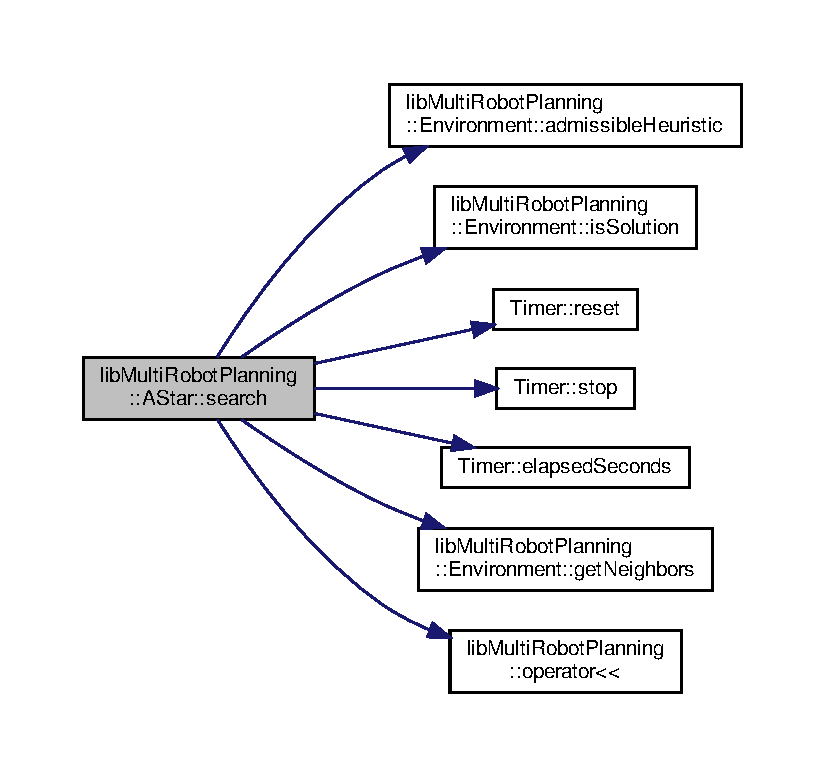
\includegraphics[width=350pt]{classlib_multi_robot_planning_1_1_a_star_acd703d42817f39d6027fa6432ca17ac9_cgraph}
\end{center}
\end{figure}
Here is the caller graph for this function\+:
\nopagebreak
\begin{figure}[H]
\begin{center}
\leavevmode
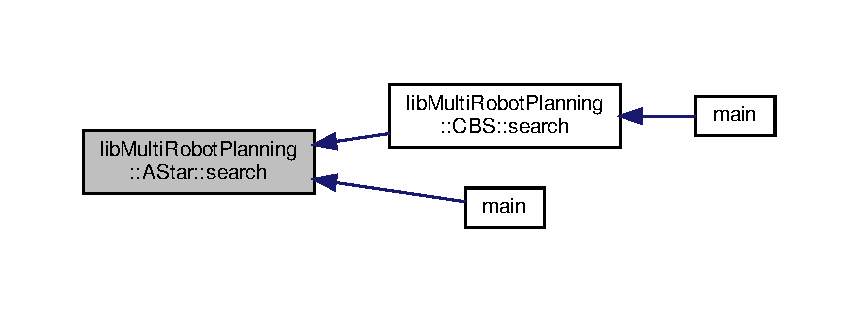
\includegraphics[width=350pt]{classlib_multi_robot_planning_1_1_a_star_acd703d42817f39d6027fa6432ca17ac9_icgraph}
\end{center}
\end{figure}


The documentation for this class was generated from the following file\+:\begin{DoxyCompactItemize}
\item 
third\+\_\+party/ecbs/include/\hyperlink{a__star_8hpp}{a\+\_\+star.\+hpp}\end{DoxyCompactItemize}

\hypertarget{classlib_multi_robot_planning_1_1_a_star_epsilon}{}\section{lib\+Multi\+Robot\+Planning\+:\+:A\+Star\+Epsilon$<$ State, Action, Cost, Environment, State\+Hasher $>$ Class Template Reference}
\label{classlib_multi_robot_planning_1_1_a_star_epsilon}\index{lib\+Multi\+Robot\+Planning\+::\+A\+Star\+Epsilon$<$ State, Action, Cost, Environment, State\+Hasher $>$@{lib\+Multi\+Robot\+Planning\+::\+A\+Star\+Epsilon$<$ State, Action, Cost, Environment, State\+Hasher $>$}}


A$\ast$\+\_\+epsilon Algorithm to find the shortest path with a given suboptimality bound (also known as focal search)  




{\ttfamily \#include $<$a\+\_\+star\+\_\+epsilon.\+hpp$>$}

\subsection*{Public Member Functions}
\begin{DoxyCompactItemize}
\item 
\hyperlink{classlib_multi_robot_planning_1_1_a_star_epsilon_a553d070b869a0d33dbbea6f0e95fee1a}{A\+Star\+Epsilon} (\hyperlink{classlib_multi_robot_planning_1_1_environment}{Environment} \&environment, float w)
\item 
bool \hyperlink{classlib_multi_robot_planning_1_1_a_star_epsilon_a24eddac1c20a92f7a58d4865b13a0186}{search} (const \hyperlink{structlib_multi_robot_planning_1_1_state}{State} \&start\+State, \hyperlink{structlib_multi_robot_planning_1_1_plan_result}{Plan\+Result}$<$ \hyperlink{structlib_multi_robot_planning_1_1_state}{State}, \hyperlink{namespacelib_multi_robot_planning_aba73fb71693f86a324adfa0e41e1053d}{Action}, Cost $>$ \&solution)
\end{DoxyCompactItemize}


\subsection{Detailed Description}
\subsubsection*{template$<$typename State, typename Action, typename Cost, typename Environment, typename State\+Hasher = std\+::hash$<$\+State$>$$>$\newline
class lib\+Multi\+Robot\+Planning\+::\+A\+Star\+Epsilon$<$ State, Action, Cost, Environment, State\+Hasher $>$}

A$\ast$\+\_\+epsilon Algorithm to find the shortest path with a given suboptimality bound (also known as focal search) 

This class implements the A$\ast$\+\_\+epsilon algorithm, an informed search algorithm that finds the shortest path for a given map up to a suboptimality factor. It uses an admissible heuristic (to keep track of the optimum) and an inadmissible heuristic ( to guide the search within a suboptimal bound w.)

Details of the algorithm can be found in the following paper\+:~\newline
Judea Pearl, Jin H. Kim\+:~\newline
\char`\"{}\+Studies in Semi-\/\+Admissible Heuristics.\char`\"{}" I\+E\+EE Trans. Pattern Anal. Mach. Intell. 4(4)\+: 392-\/399 (1982)~\newline
\href{https://doi.org/10.1109/TPAMI.1982.4767270}{\tt https\+://doi.\+org/10.\+1109/\+T\+P\+A\+M\+I.\+1982.\+4767270}

This class can either use a fibonacci heap, or a d-\/ary heap. The latter is the default. Define \char`\"{}\+U\+S\+E\+\_\+\+F\+I\+B\+O\+N\+A\+C\+C\+I\+\_\+\+H\+E\+A\+P\char`\"{} to use the fibonacci heap instead.


\begin{DoxyTemplParams}{Template Parameters}
{\em \hyperlink{structlib_multi_robot_planning_1_1_state}{State}} & Custom state for the search. Needs to be copy\textquotesingle{}able \\
\hline
{\em Action} & Custom action for the search. Needs to be copy\textquotesingle{}able \\
\hline
{\em Cost} & Custom Cost type (integer or floating point types) \\
\hline
{\em \hyperlink{classlib_multi_robot_planning_1_1_environment}{Environment}} & This class needs to provide the custom logic. In particular, it needs to support the following functions\+:
\begin{DoxyItemize}
\item {\ttfamily Cost admissible\+Heuristic(const State\& s)}~\newline
 This function can return 0 if no suitable heuristic is available.
\item {\ttfamily Cost focal\+State\+Heuristic(const State\& s, Cost g\+Score)}~\newline
 This function computes a (potentially inadmissible) heuristic for the given state.
\item {\ttfamily Cost focal\+Transition\+Heuristic(const \hyperlink{structlib_multi_robot_planning_1_1_state}{State}\& s1, const \hyperlink{structlib_multi_robot_planning_1_1_state}{State}\& s2, Cost g\+Score\+S1, Cost g\+Score\+S2)}~\newline
 This function computes a (potentially inadmissible) heuristic for the given state transition.
\item {\ttfamily bool is\+Solution(const State\& s)}~\newline
 Return true if the given state is a goal state.
\item {\ttfamily void get\+Neighbors(const \hyperlink{structlib_multi_robot_planning_1_1_state}{State}\& s, std\+::vector$<$\hyperlink{structlib_multi_robot_planning_1_1_neighbor}{Neighbor}$<$\hyperlink{structlib_multi_robot_planning_1_1_state}{State}, Action, int$>$ $>$\& neighbors)}~\newline
 Fill the list of neighboring state for the given state s.
\item {\ttfamily void on\+Expand\+Node(const State\& s, int f\+Score, int g\+Score)}~\newline
 This function is called on every expansion and can be used for statistical purposes.
\item {\ttfamily void on\+Discover(const State\& s, int f\+Score, int g\+Score)}~\newline
 This function is called on every node discovery and can be used for statistical purposes.
\end{DoxyItemize}\\
\hline
{\em State\+Hasher} & A class to convert a state to a hash value. Default\+: \hyperlink{structstd_1_1hash_3_01_state_01_4}{std\+::hash$<$\+State$>$} \\
\hline
\end{DoxyTemplParams}


Definition at line 81 of file a\+\_\+star\+\_\+epsilon.\+hpp.



\subsection{Constructor \& Destructor Documentation}
\mbox{\Hypertarget{classlib_multi_robot_planning_1_1_a_star_epsilon_a553d070b869a0d33dbbea6f0e95fee1a}\label{classlib_multi_robot_planning_1_1_a_star_epsilon_a553d070b869a0d33dbbea6f0e95fee1a}} 
\index{lib\+Multi\+Robot\+Planning\+::\+A\+Star\+Epsilon@{lib\+Multi\+Robot\+Planning\+::\+A\+Star\+Epsilon}!A\+Star\+Epsilon@{A\+Star\+Epsilon}}
\index{A\+Star\+Epsilon@{A\+Star\+Epsilon}!lib\+Multi\+Robot\+Planning\+::\+A\+Star\+Epsilon@{lib\+Multi\+Robot\+Planning\+::\+A\+Star\+Epsilon}}
\subsubsection{\texorpdfstring{A\+Star\+Epsilon()}{AStarEpsilon()}}
{\footnotesize\ttfamily template$<$typename State, typename Action, typename Cost, typename Environment, typename State\+Hasher = std\+::hash$<$\+State$>$$>$ \\
\hyperlink{classlib_multi_robot_planning_1_1_a_star_epsilon}{lib\+Multi\+Robot\+Planning\+::\+A\+Star\+Epsilon}$<$ \hyperlink{structlib_multi_robot_planning_1_1_state}{State}, \hyperlink{namespacelib_multi_robot_planning_aba73fb71693f86a324adfa0e41e1053d}{Action}, Cost, \hyperlink{classlib_multi_robot_planning_1_1_environment}{Environment}, State\+Hasher $>$\+::\hyperlink{classlib_multi_robot_planning_1_1_a_star_epsilon}{A\+Star\+Epsilon} (\begin{DoxyParamCaption}\item[{\hyperlink{classlib_multi_robot_planning_1_1_environment}{Environment} \&}]{environment,  }\item[{float}]{w }\end{DoxyParamCaption})\hspace{0.3cm}{\ttfamily [inline]}}



Definition at line 83 of file a\+\_\+star\+\_\+epsilon.\+hpp.



\subsection{Member Function Documentation}
\mbox{\Hypertarget{classlib_multi_robot_planning_1_1_a_star_epsilon_a24eddac1c20a92f7a58d4865b13a0186}\label{classlib_multi_robot_planning_1_1_a_star_epsilon_a24eddac1c20a92f7a58d4865b13a0186}} 
\index{lib\+Multi\+Robot\+Planning\+::\+A\+Star\+Epsilon@{lib\+Multi\+Robot\+Planning\+::\+A\+Star\+Epsilon}!search@{search}}
\index{search@{search}!lib\+Multi\+Robot\+Planning\+::\+A\+Star\+Epsilon@{lib\+Multi\+Robot\+Planning\+::\+A\+Star\+Epsilon}}
\subsubsection{\texorpdfstring{search()}{search()}}
{\footnotesize\ttfamily template$<$typename State, typename Action, typename Cost, typename Environment, typename State\+Hasher = std\+::hash$<$\+State$>$$>$ \\
bool \hyperlink{classlib_multi_robot_planning_1_1_a_star_epsilon}{lib\+Multi\+Robot\+Planning\+::\+A\+Star\+Epsilon}$<$ \hyperlink{structlib_multi_robot_planning_1_1_state}{State}, \hyperlink{namespacelib_multi_robot_planning_aba73fb71693f86a324adfa0e41e1053d}{Action}, Cost, \hyperlink{classlib_multi_robot_planning_1_1_environment}{Environment}, State\+Hasher $>$\+::search (\begin{DoxyParamCaption}\item[{const \hyperlink{structlib_multi_robot_planning_1_1_state}{State} \&}]{start\+State,  }\item[{\hyperlink{structlib_multi_robot_planning_1_1_plan_result}{Plan\+Result}$<$ \hyperlink{structlib_multi_robot_planning_1_1_state}{State}, \hyperlink{namespacelib_multi_robot_planning_aba73fb71693f86a324adfa0e41e1053d}{Action}, Cost $>$ \&}]{solution }\end{DoxyParamCaption})\hspace{0.3cm}{\ttfamily [inline]}}



Definition at line 86 of file a\+\_\+star\+\_\+epsilon.\+hpp.

Here is the call graph for this function\+:
\nopagebreak
\begin{figure}[H]
\begin{center}
\leavevmode
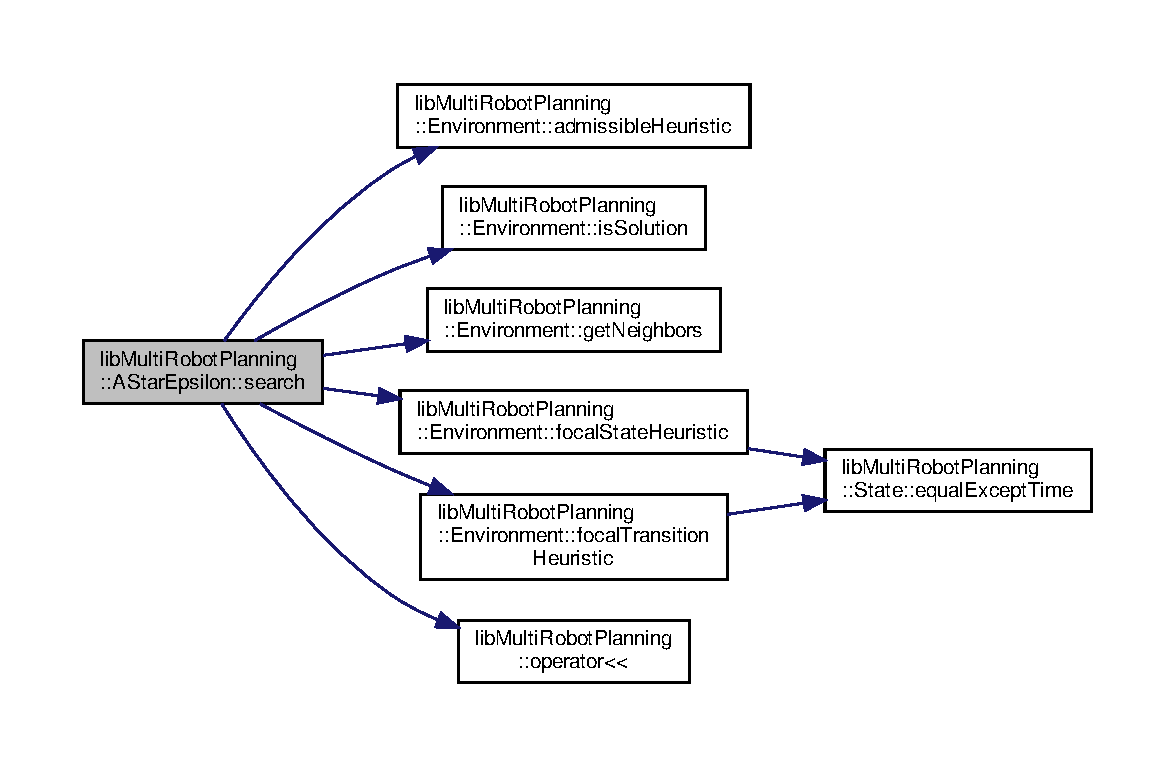
\includegraphics[width=350pt]{classlib_multi_robot_planning_1_1_a_star_epsilon_a24eddac1c20a92f7a58d4865b13a0186_cgraph}
\end{center}
\end{figure}
Here is the caller graph for this function\+:
\nopagebreak
\begin{figure}[H]
\begin{center}
\leavevmode
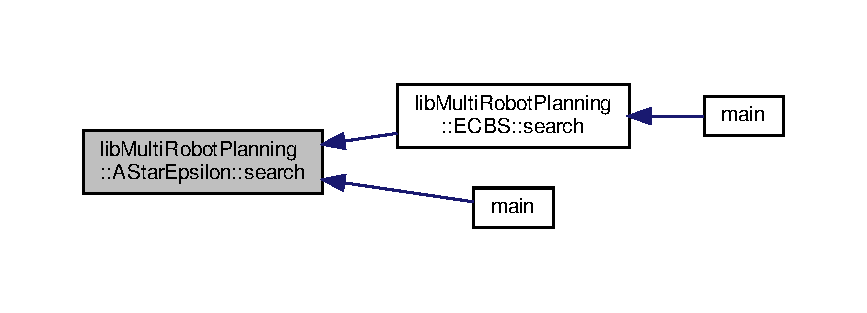
\includegraphics[width=350pt]{classlib_multi_robot_planning_1_1_a_star_epsilon_a24eddac1c20a92f7a58d4865b13a0186_icgraph}
\end{center}
\end{figure}


The documentation for this class was generated from the following file\+:\begin{DoxyCompactItemize}
\item 
third\+\_\+party/ecbs/include/\hyperlink{a__star__epsilon_8hpp}{a\+\_\+star\+\_\+epsilon.\+hpp}\end{DoxyCompactItemize}

\hypertarget{struct_box_constraint2_d}{}\section{Box\+Constraint2D Struct Reference}
\label{struct_box_constraint2_d}\index{Box\+Constraint2D@{Box\+Constraint2D}}


{\ttfamily \#include $<$corridor\+\_\+common.\+hpp$>$}

\subsection*{Public Attributes}
\begin{DoxyCompactItemize}
\item 
double \hyperlink{struct_box_constraint2_d_a29552a451142588053454d5845c595f3}{xl}
\item 
double \hyperlink{struct_box_constraint2_d_a8ae8a298620374e282506aa35dfd2248}{yl}
\item 
double \hyperlink{struct_box_constraint2_d_a1cf45ba0f8952e0d8b4fba353cc3cfff}{xu}
\item 
double \hyperlink{struct_box_constraint2_d_a250a6cb999ee308cbfe4144afdddb803}{yu}
\item 
double \hyperlink{struct_box_constraint2_d_ad7238545e4f5934bffea66b566514b8d}{t\+\_\+start}
\item 
double \hyperlink{struct_box_constraint2_d_adc1625966c4113bb5980be3db6bd3c6f}{t\+\_\+end}
\end{DoxyCompactItemize}


\subsection{Detailed Description}


Definition at line 13 of file corridor\+\_\+common.\+hpp.



\subsection{Member Data Documentation}
\mbox{\Hypertarget{struct_box_constraint2_d_adc1625966c4113bb5980be3db6bd3c6f}\label{struct_box_constraint2_d_adc1625966c4113bb5980be3db6bd3c6f}} 
\index{Box\+Constraint2D@{Box\+Constraint2D}!t\+\_\+end@{t\+\_\+end}}
\index{t\+\_\+end@{t\+\_\+end}!Box\+Constraint2D@{Box\+Constraint2D}}
\subsubsection{\texorpdfstring{t\+\_\+end}{t\_end}}
{\footnotesize\ttfamily double Box\+Constraint2\+D\+::t\+\_\+end}



Definition at line 20 of file corridor\+\_\+common.\+hpp.

\mbox{\Hypertarget{struct_box_constraint2_d_ad7238545e4f5934bffea66b566514b8d}\label{struct_box_constraint2_d_ad7238545e4f5934bffea66b566514b8d}} 
\index{Box\+Constraint2D@{Box\+Constraint2D}!t\+\_\+start@{t\+\_\+start}}
\index{t\+\_\+start@{t\+\_\+start}!Box\+Constraint2D@{Box\+Constraint2D}}
\subsubsection{\texorpdfstring{t\+\_\+start}{t\_start}}
{\footnotesize\ttfamily double Box\+Constraint2\+D\+::t\+\_\+start}



Definition at line 19 of file corridor\+\_\+common.\+hpp.

\mbox{\Hypertarget{struct_box_constraint2_d_a29552a451142588053454d5845c595f3}\label{struct_box_constraint2_d_a29552a451142588053454d5845c595f3}} 
\index{Box\+Constraint2D@{Box\+Constraint2D}!xl@{xl}}
\index{xl@{xl}!Box\+Constraint2D@{Box\+Constraint2D}}
\subsubsection{\texorpdfstring{xl}{xl}}
{\footnotesize\ttfamily double Box\+Constraint2\+D\+::xl}



Definition at line 14 of file corridor\+\_\+common.\+hpp.

\mbox{\Hypertarget{struct_box_constraint2_d_a1cf45ba0f8952e0d8b4fba353cc3cfff}\label{struct_box_constraint2_d_a1cf45ba0f8952e0d8b4fba353cc3cfff}} 
\index{Box\+Constraint2D@{Box\+Constraint2D}!xu@{xu}}
\index{xu@{xu}!Box\+Constraint2D@{Box\+Constraint2D}}
\subsubsection{\texorpdfstring{xu}{xu}}
{\footnotesize\ttfamily double Box\+Constraint2\+D\+::xu}



Definition at line 16 of file corridor\+\_\+common.\+hpp.

\mbox{\Hypertarget{struct_box_constraint2_d_a8ae8a298620374e282506aa35dfd2248}\label{struct_box_constraint2_d_a8ae8a298620374e282506aa35dfd2248}} 
\index{Box\+Constraint2D@{Box\+Constraint2D}!yl@{yl}}
\index{yl@{yl}!Box\+Constraint2D@{Box\+Constraint2D}}
\subsubsection{\texorpdfstring{yl}{yl}}
{\footnotesize\ttfamily double Box\+Constraint2\+D\+::yl}



Definition at line 15 of file corridor\+\_\+common.\+hpp.

\mbox{\Hypertarget{struct_box_constraint2_d_a250a6cb999ee308cbfe4144afdddb803}\label{struct_box_constraint2_d_a250a6cb999ee308cbfe4144afdddb803}} 
\index{Box\+Constraint2D@{Box\+Constraint2D}!yu@{yu}}
\index{yu@{yu}!Box\+Constraint2D@{Box\+Constraint2D}}
\subsubsection{\texorpdfstring{yu}{yu}}
{\footnotesize\ttfamily double Box\+Constraint2\+D\+::yu}



Definition at line 17 of file corridor\+\_\+common.\+hpp.



The documentation for this struct was generated from the following file\+:\begin{DoxyCompactItemize}
\item 
include/\hyperlink{corridor__common_8hpp}{corridor\+\_\+common.\+hpp}\end{DoxyCompactItemize}

\hypertarget{classlib_multi_robot_planning_1_1_c_b_s}{}\section{lib\+Multi\+Robot\+Planning\+:\+:C\+BS$<$ State, Action, Cost, Conflict, Constraints, Environment $>$ Class Template Reference}
\label{classlib_multi_robot_planning_1_1_c_b_s}\index{lib\+Multi\+Robot\+Planning\+::\+C\+B\+S$<$ State, Action, Cost, Conflict, Constraints, Environment $>$@{lib\+Multi\+Robot\+Planning\+::\+C\+B\+S$<$ State, Action, Cost, Conflict, Constraints, Environment $>$}}


Conflict-\/\+Based-\/\+Search (\hyperlink{classlib_multi_robot_planning_1_1_c_b_s}{C\+BS}) algorithm to solve the Multi-\/\+Agent Path-\/\+Finding (M\+A\+PF) problem.  




{\ttfamily \#include $<$cbs.\+hpp$>$}

\subsection*{Public Member Functions}
\begin{DoxyCompactItemize}
\item 
\hyperlink{classlib_multi_robot_planning_1_1_c_b_s_ad83ae3366ad3bfc2a7582ca53450ad97}{C\+BS} (\hyperlink{classlib_multi_robot_planning_1_1_environment}{Environment} \&environment)
\item 
bool \hyperlink{classlib_multi_robot_planning_1_1_c_b_s_a09eec524489ee5cfbf66c95a951d7bbe}{search} (const std\+::vector$<$ \hyperlink{structlib_multi_robot_planning_1_1_state}{State} $>$ \&initial\+States, std\+::vector$<$ \hyperlink{structlib_multi_robot_planning_1_1_plan_result}{Plan\+Result}$<$ \hyperlink{structlib_multi_robot_planning_1_1_state}{State}, \hyperlink{namespacelib_multi_robot_planning_aba73fb71693f86a324adfa0e41e1053d}{Action}, Cost $>$ $>$ \&solution)
\end{DoxyCompactItemize}


\subsection{Detailed Description}
\subsubsection*{template$<$typename State, typename Action, typename Cost, typename Conflict, typename Constraints, typename Environment$>$\newline
class lib\+Multi\+Robot\+Planning\+::\+C\+B\+S$<$ State, Action, Cost, Conflict, Constraints, Environment $>$}

Conflict-\/\+Based-\/\+Search (\hyperlink{classlib_multi_robot_planning_1_1_c_b_s}{C\+BS}) algorithm to solve the Multi-\/\+Agent Path-\/\+Finding (M\+A\+PF) problem. 

This class implements the Conflict-\/\+Based-\/\+Search (\hyperlink{classlib_multi_robot_planning_1_1_c_b_s}{C\+BS}) algorithm. This algorithm can find collision-\/free path for multiple agents with start and goal locations given for each agent. \hyperlink{classlib_multi_robot_planning_1_1_c_b_s}{C\+BS} is a two-\/level search. On the low-\/level, A$\ast$ is used to find paths for individual agents (ideally using a perfect heuristic). The high-\/level is a tree-\/search that resolves conflicts between agents as they occur, earliest conflict-\/time first. \hyperlink{classlib_multi_robot_planning_1_1_c_b_s}{C\+BS} is optimal with respect to the sum-\/of-\/individual costs.

Details of the algorithm can be found in the following paper\+:~\newline
Guni Sharon, Roni Stern, Ariel Felner, Nathan R. Sturtevant\+:~\newline
\char`\"{}\+Conflict-\/based search for optimal multi-\/agent pathfinding\char`\"{}. Artif. Intell. 219\+: 40-\/66 (2015)~\newline
\href{https://doi.org/10.1016/j.artint.2014.11.006}{\tt https\+://doi.\+org/10.\+1016/j.\+artint.\+2014.\+11.\+006}

The underlying A$\ast$ can either use a fibonacci heap, or a d-\/ary heap. The latter is the default. Define \char`\"{}\+U\+S\+E\+\_\+\+F\+I\+B\+O\+N\+A\+C\+C\+I\+\_\+\+H\+E\+A\+P\char`\"{} to use the fibonacci heap instead.


\begin{DoxyTemplParams}{Template Parameters}
{\em \hyperlink{structlib_multi_robot_planning_1_1_state}{State}} & Custom state for the search. Needs to be copy\textquotesingle{}able \\
\hline
{\em Action} & Custom action for the search. Needs to be copy\textquotesingle{}able \\
\hline
{\em Cost} & Custom Cost type (integer or floating point types) \\
\hline
{\em \hyperlink{structlib_multi_robot_planning_1_1_conflict}{Conflict}} & Custom conflict description. A conflict needs to be able to be transformed into a constraint. \\
\hline
{\em \hyperlink{structlib_multi_robot_planning_1_1_constraints}{Constraints}} & Custom constraint description. The \hyperlink{classlib_multi_robot_planning_1_1_environment}{Environment} needs to be able to search on the low-\/level while taking the constraints into account. \\
\hline
{\em \hyperlink{classlib_multi_robot_planning_1_1_environment}{Environment}} & This class needs to provide the custom logic. In particular, it needs to support the following functions\+:
\begin{DoxyItemize}
\item {\ttfamily void set\+Low\+Level\+Context(size\+\_\+t agent\+Idx, const Constraints$\ast$ constraints)}~\newline
 Set the current context to a particular agent with the given set of constraints
\item {\ttfamily Cost admissible\+Heuristic(const State\& s)}~\newline
 Admissible heuristic. Needs to take current context into account.
\item {\ttfamily bool is\+Solution(const State\& s)}~\newline
 Return true if the given state is a goal state for the current agent.
\item {\ttfamily void get\+Neighbors(const \hyperlink{structlib_multi_robot_planning_1_1_state}{State}\& s, std\+::vector$<$\hyperlink{structlib_multi_robot_planning_1_1_neighbor}{Neighbor}$<$\hyperlink{structlib_multi_robot_planning_1_1_state}{State}, Action, int$>$ $>$\& neighbors)}~\newline
 Fill the list of neighboring state for the given state s and the current agent.
\item {\ttfamily bool get\+First\+Conflict(const std\+::vector$<$\hyperlink{structlib_multi_robot_planning_1_1_plan_result}{Plan\+Result}$<$\hyperlink{structlib_multi_robot_planning_1_1_state}{State}, Action, int$>$ $>$\& solution, \hyperlink{structlib_multi_robot_planning_1_1_conflict}{Conflict}\& result)}~\newline
 Finds the first conflict for the given solution for each agent. Return true if a conflict was found and false otherwise.
\item {\ttfamily void create\+Constraints\+From\+Conflict(const \hyperlink{structlib_multi_robot_planning_1_1_conflict}{Conflict}\& conflict, std\+::map$<$size\+\_\+t, \hyperlink{structlib_multi_robot_planning_1_1_constraints}{Constraints}$>$\& constraints)}~\newline
 Create a list of constraints for the given conflict.
\item {\ttfamily void on\+Expand\+High\+Level\+Node(\+Cost cost)}~\newline
 This function is called on every high-\/level expansion and can be used for statistical purposes.
\item {\ttfamily void on\+Expand\+Low\+Level\+Node(const State\& s, Cost f\+Score, Cost g\+Score)}~\newline
 This function is called on every low-\/level expansion and can be used for statistical purposes. 
\end{DoxyItemize}\\
\hline
\end{DoxyTemplParams}


Definition at line 81 of file cbs.\+hpp.



\subsection{Constructor \& Destructor Documentation}
\mbox{\Hypertarget{classlib_multi_robot_planning_1_1_c_b_s_ad83ae3366ad3bfc2a7582ca53450ad97}\label{classlib_multi_robot_planning_1_1_c_b_s_ad83ae3366ad3bfc2a7582ca53450ad97}} 
\index{lib\+Multi\+Robot\+Planning\+::\+C\+BS@{lib\+Multi\+Robot\+Planning\+::\+C\+BS}!C\+BS@{C\+BS}}
\index{C\+BS@{C\+BS}!lib\+Multi\+Robot\+Planning\+::\+C\+BS@{lib\+Multi\+Robot\+Planning\+::\+C\+BS}}
\subsubsection{\texorpdfstring{C\+B\+S()}{CBS()}}
{\footnotesize\ttfamily template$<$typename State, typename Action, typename Cost, typename Conflict, typename Constraints, typename Environment$>$ \\
\hyperlink{classlib_multi_robot_planning_1_1_c_b_s}{lib\+Multi\+Robot\+Planning\+::\+C\+BS}$<$ \hyperlink{structlib_multi_robot_planning_1_1_state}{State}, \hyperlink{namespacelib_multi_robot_planning_aba73fb71693f86a324adfa0e41e1053d}{Action}, Cost, \hyperlink{structlib_multi_robot_planning_1_1_conflict}{Conflict}, \hyperlink{structlib_multi_robot_planning_1_1_constraints}{Constraints}, \hyperlink{classlib_multi_robot_planning_1_1_environment}{Environment} $>$\+::\hyperlink{classlib_multi_robot_planning_1_1_c_b_s}{C\+BS} (\begin{DoxyParamCaption}\item[{\hyperlink{classlib_multi_robot_planning_1_1_environment}{Environment} \&}]{environment }\end{DoxyParamCaption})\hspace{0.3cm}{\ttfamily [inline]}}



Definition at line 83 of file cbs.\+hpp.



\subsection{Member Function Documentation}
\mbox{\Hypertarget{classlib_multi_robot_planning_1_1_c_b_s_a09eec524489ee5cfbf66c95a951d7bbe}\label{classlib_multi_robot_planning_1_1_c_b_s_a09eec524489ee5cfbf66c95a951d7bbe}} 
\index{lib\+Multi\+Robot\+Planning\+::\+C\+BS@{lib\+Multi\+Robot\+Planning\+::\+C\+BS}!search@{search}}
\index{search@{search}!lib\+Multi\+Robot\+Planning\+::\+C\+BS@{lib\+Multi\+Robot\+Planning\+::\+C\+BS}}
\subsubsection{\texorpdfstring{search()}{search()}}
{\footnotesize\ttfamily template$<$typename State, typename Action, typename Cost, typename Conflict, typename Constraints, typename Environment$>$ \\
bool \hyperlink{classlib_multi_robot_planning_1_1_c_b_s}{lib\+Multi\+Robot\+Planning\+::\+C\+BS}$<$ \hyperlink{structlib_multi_robot_planning_1_1_state}{State}, \hyperlink{namespacelib_multi_robot_planning_aba73fb71693f86a324adfa0e41e1053d}{Action}, Cost, \hyperlink{structlib_multi_robot_planning_1_1_conflict}{Conflict}, \hyperlink{structlib_multi_robot_planning_1_1_constraints}{Constraints}, \hyperlink{classlib_multi_robot_planning_1_1_environment}{Environment} $>$\+::search (\begin{DoxyParamCaption}\item[{const std\+::vector$<$ \hyperlink{structlib_multi_robot_planning_1_1_state}{State} $>$ \&}]{initial\+States,  }\item[{std\+::vector$<$ \hyperlink{structlib_multi_robot_planning_1_1_plan_result}{Plan\+Result}$<$ \hyperlink{structlib_multi_robot_planning_1_1_state}{State}, \hyperlink{namespacelib_multi_robot_planning_aba73fb71693f86a324adfa0e41e1053d}{Action}, Cost $>$ $>$ \&}]{solution }\end{DoxyParamCaption})\hspace{0.3cm}{\ttfamily [inline]}}



Definition at line 85 of file cbs.\+hpp.

Here is the call graph for this function\+:
\nopagebreak
\begin{figure}[H]
\begin{center}
\leavevmode
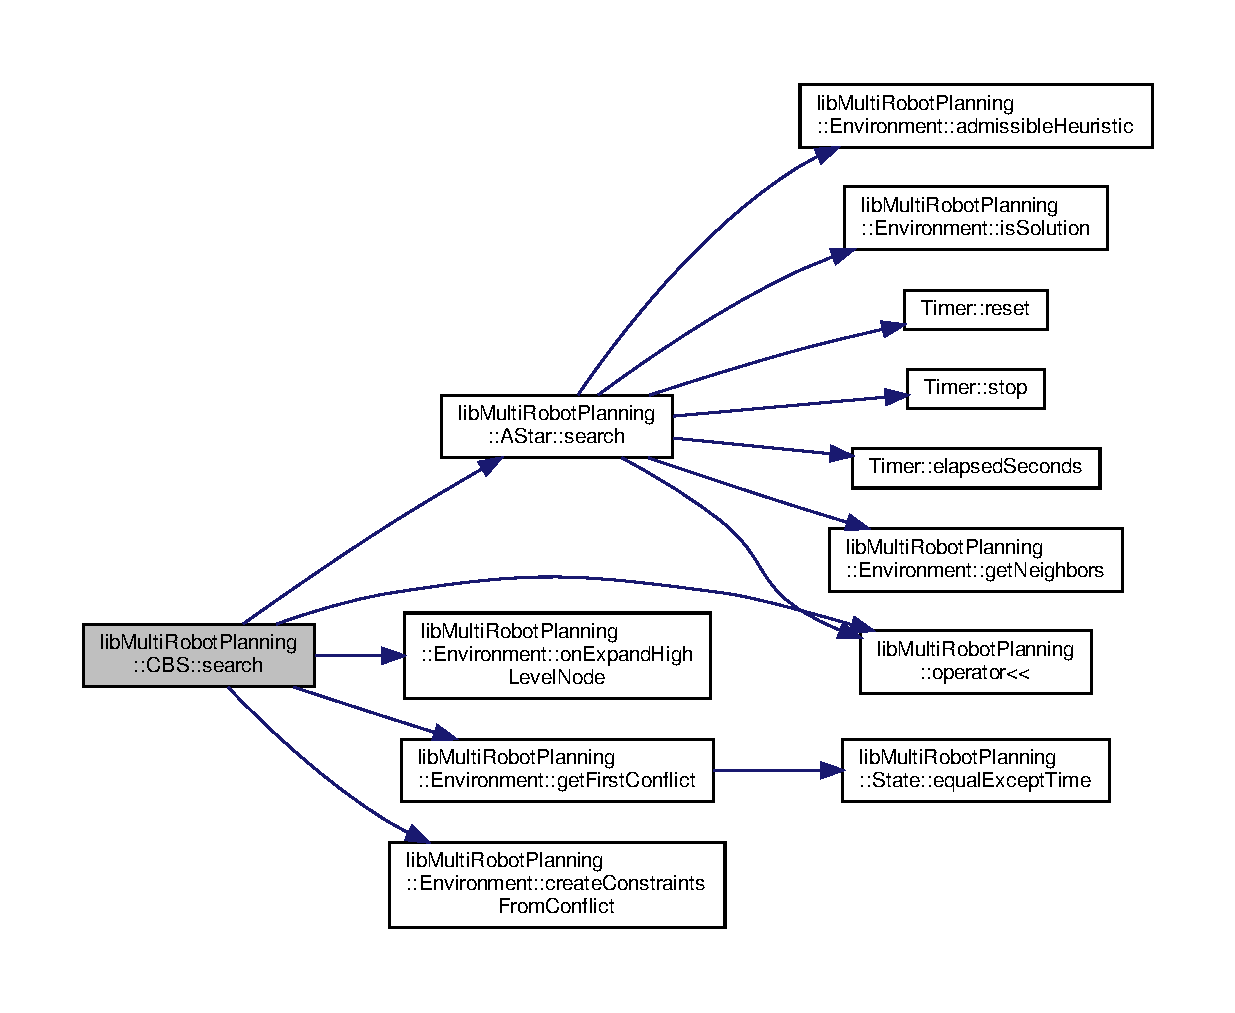
\includegraphics[width=350pt]{classlib_multi_robot_planning_1_1_c_b_s_a09eec524489ee5cfbf66c95a951d7bbe_cgraph}
\end{center}
\end{figure}
Here is the caller graph for this function\+:
\nopagebreak
\begin{figure}[H]
\begin{center}
\leavevmode
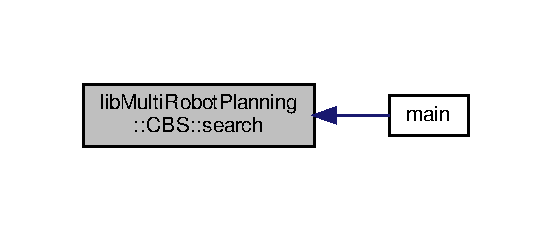
\includegraphics[width=265pt]{classlib_multi_robot_planning_1_1_c_b_s_a09eec524489ee5cfbf66c95a951d7bbe_icgraph}
\end{center}
\end{figure}


The documentation for this class was generated from the following file\+:\begin{DoxyCompactItemize}
\item 
third\+\_\+party/ecbs/include/\hyperlink{cbs_8hpp}{cbs.\+hpp}\end{DoxyCompactItemize}

\hypertarget{struct_conflict}{}\section{Conflict Struct Reference}
\label{struct_conflict}\index{Conflict@{Conflict}}
\subsection*{Public Types}
\begin{DoxyCompactItemize}
\item 
enum \hyperlink{struct_conflict_aee4228c4b31f415064213a2bbebe3eb6}{Type} \{ \hyperlink{struct_conflict_aee4228c4b31f415064213a2bbebe3eb6ab8d89ab66862b11dc349e54eddbe1228}{Vertex}, 
\hyperlink{struct_conflict_aee4228c4b31f415064213a2bbebe3eb6a26aa4d7e034987c2d348684b8a3dfdca}{Edge}, 
\hyperlink{struct_conflict_aee4228c4b31f415064213a2bbebe3eb6ab8d89ab66862b11dc349e54eddbe1228}{Vertex}, 
\hyperlink{struct_conflict_aee4228c4b31f415064213a2bbebe3eb6a26aa4d7e034987c2d348684b8a3dfdca}{Edge}
 \}
\item 
enum \hyperlink{struct_conflict_aee4228c4b31f415064213a2bbebe3eb6}{Type} \{ \hyperlink{struct_conflict_aee4228c4b31f415064213a2bbebe3eb6ab8d89ab66862b11dc349e54eddbe1228}{Vertex}, 
\hyperlink{struct_conflict_aee4228c4b31f415064213a2bbebe3eb6a26aa4d7e034987c2d348684b8a3dfdca}{Edge}, 
\hyperlink{struct_conflict_aee4228c4b31f415064213a2bbebe3eb6ab8d89ab66862b11dc349e54eddbe1228}{Vertex}, 
\hyperlink{struct_conflict_aee4228c4b31f415064213a2bbebe3eb6a26aa4d7e034987c2d348684b8a3dfdca}{Edge}
 \}
\end{DoxyCompactItemize}
\subsection*{Public Attributes}
\begin{DoxyCompactItemize}
\item 
int \hyperlink{struct_conflict_a1c5e5967fe6b6f20a67910df06a4133f}{time}
\item 
size\+\_\+t \hyperlink{struct_conflict_a202c78783691564fb2a576d1bd6fe0b5}{agent1}
\item 
size\+\_\+t \hyperlink{struct_conflict_ad8ecb104ed7c27c703e26187d96defa6}{agent2}
\item 
\hyperlink{struct_conflict_aee4228c4b31f415064213a2bbebe3eb6}{Type} \hyperlink{struct_conflict_acf201248af61ee8fad8e1e806df12172}{type}
\item 
int \hyperlink{struct_conflict_a9a1d3928989b17b8c5785a6d7fd335fa}{x1}
\item 
int \hyperlink{struct_conflict_a48f6033f035b152132cbbc0081a9216b}{y1}
\item 
int \hyperlink{struct_conflict_ab5d52bb95d71415d8154c0d9271b703c}{z1}
\item 
int \hyperlink{struct_conflict_a8a31ca7b4e951e2fc111def844b81d7e}{x2}
\item 
int \hyperlink{struct_conflict_aa0406a6a50889d8c1803b6ec11c21230}{y2}
\item 
int \hyperlink{struct_conflict_afd42fecf78db0ec2a73bc9eadc554960}{z2}
\end{DoxyCompactItemize}
\subsection*{Friends}
\begin{DoxyCompactItemize}
\item 
std\+::ostream \& \hyperlink{struct_conflict_a0fda4f63e0d8129b08d7b15bd2d6fb82}{operator$<$$<$} (std\+::ostream \&os, const \hyperlink{struct_conflict}{Conflict} \&c)
\item 
std\+::ostream \& \hyperlink{struct_conflict_a0fda4f63e0d8129b08d7b15bd2d6fb82}{operator$<$$<$} (std\+::ostream \&os, const \hyperlink{struct_conflict}{Conflict} \&c)
\end{DoxyCompactItemize}


\subsection{Detailed Description}


Definition at line 90 of file cbs.\+cpp.



\subsection{Member Enumeration Documentation}
\mbox{\Hypertarget{struct_conflict_aee4228c4b31f415064213a2bbebe3eb6}\label{struct_conflict_aee4228c4b31f415064213a2bbebe3eb6}} 
\index{Conflict@{Conflict}!Type@{Type}}
\index{Type@{Type}!Conflict@{Conflict}}
\subsubsection{\texorpdfstring{Type}{Type}\hspace{0.1cm}{\footnotesize\ttfamily [1/2]}}
{\footnotesize\ttfamily enum \hyperlink{struct_conflict_aee4228c4b31f415064213a2bbebe3eb6}{Conflict\+::\+Type}}

\begin{DoxyEnumFields}{Enumerator}
\raisebox{\heightof{T}}[0pt][0pt]{\index{Vertex@{Vertex}!Conflict@{Conflict}}\index{Conflict@{Conflict}!Vertex@{Vertex}}}\mbox{\Hypertarget{struct_conflict_aee4228c4b31f415064213a2bbebe3eb6ab8d89ab66862b11dc349e54eddbe1228}\label{struct_conflict_aee4228c4b31f415064213a2bbebe3eb6ab8d89ab66862b11dc349e54eddbe1228}} 
Vertex&\\
\hline

\raisebox{\heightof{T}}[0pt][0pt]{\index{Edge@{Edge}!Conflict@{Conflict}}\index{Conflict@{Conflict}!Edge@{Edge}}}\mbox{\Hypertarget{struct_conflict_aee4228c4b31f415064213a2bbebe3eb6a26aa4d7e034987c2d348684b8a3dfdca}\label{struct_conflict_aee4228c4b31f415064213a2bbebe3eb6a26aa4d7e034987c2d348684b8a3dfdca}} 
Edge&\\
\hline

\raisebox{\heightof{T}}[0pt][0pt]{\index{Vertex@{Vertex}!Conflict@{Conflict}}\index{Conflict@{Conflict}!Vertex@{Vertex}}}\mbox{\Hypertarget{struct_conflict_aee4228c4b31f415064213a2bbebe3eb6ab8d89ab66862b11dc349e54eddbe1228}\label{struct_conflict_aee4228c4b31f415064213a2bbebe3eb6ab8d89ab66862b11dc349e54eddbe1228}} 
Vertex&\\
\hline

\raisebox{\heightof{T}}[0pt][0pt]{\index{Edge@{Edge}!Conflict@{Conflict}}\index{Conflict@{Conflict}!Edge@{Edge}}}\mbox{\Hypertarget{struct_conflict_aee4228c4b31f415064213a2bbebe3eb6a26aa4d7e034987c2d348684b8a3dfdca}\label{struct_conflict_aee4228c4b31f415064213a2bbebe3eb6a26aa4d7e034987c2d348684b8a3dfdca}} 
Edge&\\
\hline

\end{DoxyEnumFields}


Definition at line 91 of file cbs.\+cpp.

\mbox{\Hypertarget{struct_conflict_aee4228c4b31f415064213a2bbebe3eb6}\label{struct_conflict_aee4228c4b31f415064213a2bbebe3eb6}} 
\index{Conflict@{Conflict}!Type@{Type}}
\index{Type@{Type}!Conflict@{Conflict}}
\subsubsection{\texorpdfstring{Type}{Type}\hspace{0.1cm}{\footnotesize\ttfamily [2/2]}}
{\footnotesize\ttfamily enum \hyperlink{struct_conflict_aee4228c4b31f415064213a2bbebe3eb6}{Conflict\+::\+Type}}

\begin{DoxyEnumFields}{Enumerator}
\raisebox{\heightof{T}}[0pt][0pt]{\index{Vertex@{Vertex}!Conflict@{Conflict}}\index{Conflict@{Conflict}!Vertex@{Vertex}}}\mbox{\Hypertarget{struct_conflict_aee4228c4b31f415064213a2bbebe3eb6ab8d89ab66862b11dc349e54eddbe1228}\label{struct_conflict_aee4228c4b31f415064213a2bbebe3eb6ab8d89ab66862b11dc349e54eddbe1228}} 
Vertex&\\
\hline

\raisebox{\heightof{T}}[0pt][0pt]{\index{Edge@{Edge}!Conflict@{Conflict}}\index{Conflict@{Conflict}!Edge@{Edge}}}\mbox{\Hypertarget{struct_conflict_aee4228c4b31f415064213a2bbebe3eb6a26aa4d7e034987c2d348684b8a3dfdca}\label{struct_conflict_aee4228c4b31f415064213a2bbebe3eb6a26aa4d7e034987c2d348684b8a3dfdca}} 
Edge&\\
\hline

\raisebox{\heightof{T}}[0pt][0pt]{\index{Vertex@{Vertex}!Conflict@{Conflict}}\index{Conflict@{Conflict}!Vertex@{Vertex}}}\mbox{\Hypertarget{struct_conflict_aee4228c4b31f415064213a2bbebe3eb6ab8d89ab66862b11dc349e54eddbe1228}\label{struct_conflict_aee4228c4b31f415064213a2bbebe3eb6ab8d89ab66862b11dc349e54eddbe1228}} 
Vertex&\\
\hline

\raisebox{\heightof{T}}[0pt][0pt]{\index{Edge@{Edge}!Conflict@{Conflict}}\index{Conflict@{Conflict}!Edge@{Edge}}}\mbox{\Hypertarget{struct_conflict_aee4228c4b31f415064213a2bbebe3eb6a26aa4d7e034987c2d348684b8a3dfdca}\label{struct_conflict_aee4228c4b31f415064213a2bbebe3eb6a26aa4d7e034987c2d348684b8a3dfdca}} 
Edge&\\
\hline

\end{DoxyEnumFields}


Definition at line 91 of file ecbs.\+cpp.



\subsection{Friends And Related Function Documentation}
\mbox{\Hypertarget{struct_conflict_a0fda4f63e0d8129b08d7b15bd2d6fb82}\label{struct_conflict_a0fda4f63e0d8129b08d7b15bd2d6fb82}} 
\index{Conflict@{Conflict}!operator$<$$<$@{operator$<$$<$}}
\index{operator$<$$<$@{operator$<$$<$}!Conflict@{Conflict}}
\subsubsection{\texorpdfstring{operator$<$$<$}{operator<<}\hspace{0.1cm}{\footnotesize\ttfamily [1/2]}}
{\footnotesize\ttfamily std\+::ostream\& operator$<$$<$ (\begin{DoxyParamCaption}\item[{std\+::ostream \&}]{os,  }\item[{const \hyperlink{struct_conflict}{Conflict} \&}]{c }\end{DoxyParamCaption})\hspace{0.3cm}{\ttfamily [friend]}}



Definition at line 108 of file cbs.\+cpp.

\mbox{\Hypertarget{struct_conflict_a0fda4f63e0d8129b08d7b15bd2d6fb82}\label{struct_conflict_a0fda4f63e0d8129b08d7b15bd2d6fb82}} 
\index{Conflict@{Conflict}!operator$<$$<$@{operator$<$$<$}}
\index{operator$<$$<$@{operator$<$$<$}!Conflict@{Conflict}}
\subsubsection{\texorpdfstring{operator$<$$<$}{operator<<}\hspace{0.1cm}{\footnotesize\ttfamily [2/2]}}
{\footnotesize\ttfamily std\+::ostream\& operator$<$$<$ (\begin{DoxyParamCaption}\item[{std\+::ostream \&}]{os,  }\item[{const \hyperlink{struct_conflict}{Conflict} \&}]{c }\end{DoxyParamCaption})\hspace{0.3cm}{\ttfamily [friend]}}



Definition at line 108 of file ecbs.\+cpp.



\subsection{Member Data Documentation}
\mbox{\Hypertarget{struct_conflict_a202c78783691564fb2a576d1bd6fe0b5}\label{struct_conflict_a202c78783691564fb2a576d1bd6fe0b5}} 
\index{Conflict@{Conflict}!agent1@{agent1}}
\index{agent1@{agent1}!Conflict@{Conflict}}
\subsubsection{\texorpdfstring{agent1}{agent1}}
{\footnotesize\ttfamily size\+\_\+t Conflict\+::agent1}



Definition at line 97 of file cbs.\+cpp.

\mbox{\Hypertarget{struct_conflict_ad8ecb104ed7c27c703e26187d96defa6}\label{struct_conflict_ad8ecb104ed7c27c703e26187d96defa6}} 
\index{Conflict@{Conflict}!agent2@{agent2}}
\index{agent2@{agent2}!Conflict@{Conflict}}
\subsubsection{\texorpdfstring{agent2}{agent2}}
{\footnotesize\ttfamily size\+\_\+t Conflict\+::agent2}



Definition at line 98 of file cbs.\+cpp.

\mbox{\Hypertarget{struct_conflict_a1c5e5967fe6b6f20a67910df06a4133f}\label{struct_conflict_a1c5e5967fe6b6f20a67910df06a4133f}} 
\index{Conflict@{Conflict}!time@{time}}
\index{time@{time}!Conflict@{Conflict}}
\subsubsection{\texorpdfstring{time}{time}}
{\footnotesize\ttfamily int Conflict\+::time}



Definition at line 96 of file cbs.\+cpp.

\mbox{\Hypertarget{struct_conflict_acf201248af61ee8fad8e1e806df12172}\label{struct_conflict_acf201248af61ee8fad8e1e806df12172}} 
\index{Conflict@{Conflict}!type@{type}}
\index{type@{type}!Conflict@{Conflict}}
\subsubsection{\texorpdfstring{type}{type}}
{\footnotesize\ttfamily \hyperlink{struct_conflict_aee4228c4b31f415064213a2bbebe3eb6}{Type} Conflict\+::type}



Definition at line 99 of file cbs.\+cpp.

\mbox{\Hypertarget{struct_conflict_a9a1d3928989b17b8c5785a6d7fd335fa}\label{struct_conflict_a9a1d3928989b17b8c5785a6d7fd335fa}} 
\index{Conflict@{Conflict}!x1@{x1}}
\index{x1@{x1}!Conflict@{Conflict}}
\subsubsection{\texorpdfstring{x1}{x1}}
{\footnotesize\ttfamily int Conflict\+::x1}



Definition at line 101 of file cbs.\+cpp.

\mbox{\Hypertarget{struct_conflict_a8a31ca7b4e951e2fc111def844b81d7e}\label{struct_conflict_a8a31ca7b4e951e2fc111def844b81d7e}} 
\index{Conflict@{Conflict}!x2@{x2}}
\index{x2@{x2}!Conflict@{Conflict}}
\subsubsection{\texorpdfstring{x2}{x2}}
{\footnotesize\ttfamily int Conflict\+::x2}



Definition at line 104 of file cbs.\+cpp.

\mbox{\Hypertarget{struct_conflict_a48f6033f035b152132cbbc0081a9216b}\label{struct_conflict_a48f6033f035b152132cbbc0081a9216b}} 
\index{Conflict@{Conflict}!y1@{y1}}
\index{y1@{y1}!Conflict@{Conflict}}
\subsubsection{\texorpdfstring{y1}{y1}}
{\footnotesize\ttfamily int Conflict\+::y1}



Definition at line 102 of file cbs.\+cpp.

\mbox{\Hypertarget{struct_conflict_aa0406a6a50889d8c1803b6ec11c21230}\label{struct_conflict_aa0406a6a50889d8c1803b6ec11c21230}} 
\index{Conflict@{Conflict}!y2@{y2}}
\index{y2@{y2}!Conflict@{Conflict}}
\subsubsection{\texorpdfstring{y2}{y2}}
{\footnotesize\ttfamily int Conflict\+::y2}



Definition at line 105 of file cbs.\+cpp.

\mbox{\Hypertarget{struct_conflict_ab5d52bb95d71415d8154c0d9271b703c}\label{struct_conflict_ab5d52bb95d71415d8154c0d9271b703c}} 
\index{Conflict@{Conflict}!z1@{z1}}
\index{z1@{z1}!Conflict@{Conflict}}
\subsubsection{\texorpdfstring{z1}{z1}}
{\footnotesize\ttfamily int Conflict\+::z1}



Definition at line 103 of file cbs.\+cpp.

\mbox{\Hypertarget{struct_conflict_afd42fecf78db0ec2a73bc9eadc554960}\label{struct_conflict_afd42fecf78db0ec2a73bc9eadc554960}} 
\index{Conflict@{Conflict}!z2@{z2}}
\index{z2@{z2}!Conflict@{Conflict}}
\subsubsection{\texorpdfstring{z2}{z2}}
{\footnotesize\ttfamily int Conflict\+::z2}



Definition at line 106 of file cbs.\+cpp.



The documentation for this struct was generated from the following files\+:\begin{DoxyCompactItemize}
\item 
third\+\_\+party/ecbs/src/\hyperlink{cbs_8cpp}{cbs.\+cpp}\item 
third\+\_\+party/ecbs/src/\hyperlink{ecbs_8cpp}{ecbs.\+cpp}\end{DoxyCompactItemize}

\hypertarget{structlib_multi_robot_planning_1_1_conflict}{}\section{lib\+Multi\+Robot\+Planning\+:\+:Conflict Struct Reference}
\label{structlib_multi_robot_planning_1_1_conflict}\index{lib\+Multi\+Robot\+Planning\+::\+Conflict@{lib\+Multi\+Robot\+Planning\+::\+Conflict}}


{\ttfamily \#include $<$environment.\+hpp$>$}

\subsection*{Public Types}
\begin{DoxyCompactItemize}
\item 
enum \hyperlink{structlib_multi_robot_planning_1_1_conflict_a3296f220687e49565bb9b551140d5904}{Type} \{ \hyperlink{structlib_multi_robot_planning_1_1_conflict_a3296f220687e49565bb9b551140d5904a87317dee2845549dc29f55c46d23b6dc}{Vertex}, 
\hyperlink{structlib_multi_robot_planning_1_1_conflict_a3296f220687e49565bb9b551140d5904a4728181e728582a2106b599737d4016f}{Edge}
 \}
\end{DoxyCompactItemize}
\subsection*{Public Attributes}
\begin{DoxyCompactItemize}
\item 
int \hyperlink{structlib_multi_robot_planning_1_1_conflict_a086ff6e223b9b10297feba997e96b0aa}{time}
\item 
size\+\_\+t \hyperlink{structlib_multi_robot_planning_1_1_conflict_a59ad0af44ab7de8e34bb54f959b0f7af}{agent1}
\item 
size\+\_\+t \hyperlink{structlib_multi_robot_planning_1_1_conflict_a057f32689f5438209cb8450062ff9fc8}{agent2}
\item 
\hyperlink{structlib_multi_robot_planning_1_1_conflict_a3296f220687e49565bb9b551140d5904}{Type} \hyperlink{structlib_multi_robot_planning_1_1_conflict_ae655db1168c2626d11a663545d41c347}{type}
\item 
int \hyperlink{structlib_multi_robot_planning_1_1_conflict_aa0e8acc26afa57b4888161ef07d7d85a}{x1}
\item 
int \hyperlink{structlib_multi_robot_planning_1_1_conflict_a3ba25bd4fe269ead33b35c1312a02dfb}{y1}
\item 
int \hyperlink{structlib_multi_robot_planning_1_1_conflict_a439430d239251d3d3367a6261907c194}{z1}
\item 
int \hyperlink{structlib_multi_robot_planning_1_1_conflict_ab42ee87616eb071549218cf8af8aa11e}{x2}
\item 
int \hyperlink{structlib_multi_robot_planning_1_1_conflict_a257b0810cb6664aa422c713a49467d7c}{y2}
\item 
int \hyperlink{structlib_multi_robot_planning_1_1_conflict_a435f1f9f9b274d51133d137985761289}{z2}
\item 
int \hyperlink{structlib_multi_robot_planning_1_1_conflict_a85dfd0cb84314e7c3a8ccd4a3f18c565}{x3}
\item 
int \hyperlink{structlib_multi_robot_planning_1_1_conflict_a2791bab0aefef75112040cc03cd965ad}{y3}
\item 
int \hyperlink{structlib_multi_robot_planning_1_1_conflict_a0704de0fe48fcb194b46fc9fd0fcac3b}{z3}
\end{DoxyCompactItemize}
\subsection*{Friends}
\begin{DoxyCompactItemize}
\item 
std\+::ostream \& \hyperlink{structlib_multi_robot_planning_1_1_conflict_a0fda4f63e0d8129b08d7b15bd2d6fb82}{operator$<$$<$} (std\+::ostream \&os, const \hyperlink{structlib_multi_robot_planning_1_1_conflict}{Conflict} \&c)
\end{DoxyCompactItemize}


\subsection{Detailed Description}


Definition at line 90 of file environment.\+hpp.



\subsection{Member Enumeration Documentation}
\mbox{\Hypertarget{structlib_multi_robot_planning_1_1_conflict_a3296f220687e49565bb9b551140d5904}\label{structlib_multi_robot_planning_1_1_conflict_a3296f220687e49565bb9b551140d5904}} 
\index{lib\+Multi\+Robot\+Planning\+::\+Conflict@{lib\+Multi\+Robot\+Planning\+::\+Conflict}!Type@{Type}}
\index{Type@{Type}!lib\+Multi\+Robot\+Planning\+::\+Conflict@{lib\+Multi\+Robot\+Planning\+::\+Conflict}}
\subsubsection{\texorpdfstring{Type}{Type}}
{\footnotesize\ttfamily enum \hyperlink{structlib_multi_robot_planning_1_1_conflict_a3296f220687e49565bb9b551140d5904}{lib\+Multi\+Robot\+Planning\+::\+Conflict\+::\+Type}}

\begin{DoxyEnumFields}{Enumerator}
\raisebox{\heightof{T}}[0pt][0pt]{\index{Vertex@{Vertex}!lib\+Multi\+Robot\+Planning\+::\+Conflict@{lib\+Multi\+Robot\+Planning\+::\+Conflict}}\index{lib\+Multi\+Robot\+Planning\+::\+Conflict@{lib\+Multi\+Robot\+Planning\+::\+Conflict}!Vertex@{Vertex}}}\mbox{\Hypertarget{structlib_multi_robot_planning_1_1_conflict_a3296f220687e49565bb9b551140d5904a87317dee2845549dc29f55c46d23b6dc}\label{structlib_multi_robot_planning_1_1_conflict_a3296f220687e49565bb9b551140d5904a87317dee2845549dc29f55c46d23b6dc}} 
Vertex&\\
\hline

\raisebox{\heightof{T}}[0pt][0pt]{\index{Edge@{Edge}!lib\+Multi\+Robot\+Planning\+::\+Conflict@{lib\+Multi\+Robot\+Planning\+::\+Conflict}}\index{lib\+Multi\+Robot\+Planning\+::\+Conflict@{lib\+Multi\+Robot\+Planning\+::\+Conflict}!Edge@{Edge}}}\mbox{\Hypertarget{structlib_multi_robot_planning_1_1_conflict_a3296f220687e49565bb9b551140d5904a4728181e728582a2106b599737d4016f}\label{structlib_multi_robot_planning_1_1_conflict_a3296f220687e49565bb9b551140d5904a4728181e728582a2106b599737d4016f}} 
Edge&\\
\hline

\end{DoxyEnumFields}


Definition at line 91 of file environment.\+hpp.



\subsection{Friends And Related Function Documentation}
\mbox{\Hypertarget{structlib_multi_robot_planning_1_1_conflict_a0fda4f63e0d8129b08d7b15bd2d6fb82}\label{structlib_multi_robot_planning_1_1_conflict_a0fda4f63e0d8129b08d7b15bd2d6fb82}} 
\index{lib\+Multi\+Robot\+Planning\+::\+Conflict@{lib\+Multi\+Robot\+Planning\+::\+Conflict}!operator$<$$<$@{operator$<$$<$}}
\index{operator$<$$<$@{operator$<$$<$}!lib\+Multi\+Robot\+Planning\+::\+Conflict@{lib\+Multi\+Robot\+Planning\+::\+Conflict}}
\subsubsection{\texorpdfstring{operator$<$$<$}{operator<<}}
{\footnotesize\ttfamily std\+::ostream\& operator$<$$<$ (\begin{DoxyParamCaption}\item[{std\+::ostream \&}]{os,  }\item[{const \hyperlink{structlib_multi_robot_planning_1_1_conflict}{Conflict} \&}]{c }\end{DoxyParamCaption})\hspace{0.3cm}{\ttfamily [friend]}}



Definition at line 111 of file environment.\+hpp.



\subsection{Member Data Documentation}
\mbox{\Hypertarget{structlib_multi_robot_planning_1_1_conflict_a59ad0af44ab7de8e34bb54f959b0f7af}\label{structlib_multi_robot_planning_1_1_conflict_a59ad0af44ab7de8e34bb54f959b0f7af}} 
\index{lib\+Multi\+Robot\+Planning\+::\+Conflict@{lib\+Multi\+Robot\+Planning\+::\+Conflict}!agent1@{agent1}}
\index{agent1@{agent1}!lib\+Multi\+Robot\+Planning\+::\+Conflict@{lib\+Multi\+Robot\+Planning\+::\+Conflict}}
\subsubsection{\texorpdfstring{agent1}{agent1}}
{\footnotesize\ttfamily size\+\_\+t lib\+Multi\+Robot\+Planning\+::\+Conflict\+::agent1}



Definition at line 97 of file environment.\+hpp.

\mbox{\Hypertarget{structlib_multi_robot_planning_1_1_conflict_a057f32689f5438209cb8450062ff9fc8}\label{structlib_multi_robot_planning_1_1_conflict_a057f32689f5438209cb8450062ff9fc8}} 
\index{lib\+Multi\+Robot\+Planning\+::\+Conflict@{lib\+Multi\+Robot\+Planning\+::\+Conflict}!agent2@{agent2}}
\index{agent2@{agent2}!lib\+Multi\+Robot\+Planning\+::\+Conflict@{lib\+Multi\+Robot\+Planning\+::\+Conflict}}
\subsubsection{\texorpdfstring{agent2}{agent2}}
{\footnotesize\ttfamily size\+\_\+t lib\+Multi\+Robot\+Planning\+::\+Conflict\+::agent2}



Definition at line 98 of file environment.\+hpp.

\mbox{\Hypertarget{structlib_multi_robot_planning_1_1_conflict_a086ff6e223b9b10297feba997e96b0aa}\label{structlib_multi_robot_planning_1_1_conflict_a086ff6e223b9b10297feba997e96b0aa}} 
\index{lib\+Multi\+Robot\+Planning\+::\+Conflict@{lib\+Multi\+Robot\+Planning\+::\+Conflict}!time@{time}}
\index{time@{time}!lib\+Multi\+Robot\+Planning\+::\+Conflict@{lib\+Multi\+Robot\+Planning\+::\+Conflict}}
\subsubsection{\texorpdfstring{time}{time}}
{\footnotesize\ttfamily int lib\+Multi\+Robot\+Planning\+::\+Conflict\+::time}



Definition at line 96 of file environment.\+hpp.

\mbox{\Hypertarget{structlib_multi_robot_planning_1_1_conflict_ae655db1168c2626d11a663545d41c347}\label{structlib_multi_robot_planning_1_1_conflict_ae655db1168c2626d11a663545d41c347}} 
\index{lib\+Multi\+Robot\+Planning\+::\+Conflict@{lib\+Multi\+Robot\+Planning\+::\+Conflict}!type@{type}}
\index{type@{type}!lib\+Multi\+Robot\+Planning\+::\+Conflict@{lib\+Multi\+Robot\+Planning\+::\+Conflict}}
\subsubsection{\texorpdfstring{type}{type}}
{\footnotesize\ttfamily \hyperlink{structlib_multi_robot_planning_1_1_conflict_a3296f220687e49565bb9b551140d5904}{Type} lib\+Multi\+Robot\+Planning\+::\+Conflict\+::type}



Definition at line 99 of file environment.\+hpp.

\mbox{\Hypertarget{structlib_multi_robot_planning_1_1_conflict_aa0e8acc26afa57b4888161ef07d7d85a}\label{structlib_multi_robot_planning_1_1_conflict_aa0e8acc26afa57b4888161ef07d7d85a}} 
\index{lib\+Multi\+Robot\+Planning\+::\+Conflict@{lib\+Multi\+Robot\+Planning\+::\+Conflict}!x1@{x1}}
\index{x1@{x1}!lib\+Multi\+Robot\+Planning\+::\+Conflict@{lib\+Multi\+Robot\+Planning\+::\+Conflict}}
\subsubsection{\texorpdfstring{x1}{x1}}
{\footnotesize\ttfamily int lib\+Multi\+Robot\+Planning\+::\+Conflict\+::x1}



Definition at line 101 of file environment.\+hpp.

\mbox{\Hypertarget{structlib_multi_robot_planning_1_1_conflict_ab42ee87616eb071549218cf8af8aa11e}\label{structlib_multi_robot_planning_1_1_conflict_ab42ee87616eb071549218cf8af8aa11e}} 
\index{lib\+Multi\+Robot\+Planning\+::\+Conflict@{lib\+Multi\+Robot\+Planning\+::\+Conflict}!x2@{x2}}
\index{x2@{x2}!lib\+Multi\+Robot\+Planning\+::\+Conflict@{lib\+Multi\+Robot\+Planning\+::\+Conflict}}
\subsubsection{\texorpdfstring{x2}{x2}}
{\footnotesize\ttfamily int lib\+Multi\+Robot\+Planning\+::\+Conflict\+::x2}



Definition at line 104 of file environment.\+hpp.

\mbox{\Hypertarget{structlib_multi_robot_planning_1_1_conflict_a85dfd0cb84314e7c3a8ccd4a3f18c565}\label{structlib_multi_robot_planning_1_1_conflict_a85dfd0cb84314e7c3a8ccd4a3f18c565}} 
\index{lib\+Multi\+Robot\+Planning\+::\+Conflict@{lib\+Multi\+Robot\+Planning\+::\+Conflict}!x3@{x3}}
\index{x3@{x3}!lib\+Multi\+Robot\+Planning\+::\+Conflict@{lib\+Multi\+Robot\+Planning\+::\+Conflict}}
\subsubsection{\texorpdfstring{x3}{x3}}
{\footnotesize\ttfamily int lib\+Multi\+Robot\+Planning\+::\+Conflict\+::x3}



Definition at line 107 of file environment.\+hpp.

\mbox{\Hypertarget{structlib_multi_robot_planning_1_1_conflict_a3ba25bd4fe269ead33b35c1312a02dfb}\label{structlib_multi_robot_planning_1_1_conflict_a3ba25bd4fe269ead33b35c1312a02dfb}} 
\index{lib\+Multi\+Robot\+Planning\+::\+Conflict@{lib\+Multi\+Robot\+Planning\+::\+Conflict}!y1@{y1}}
\index{y1@{y1}!lib\+Multi\+Robot\+Planning\+::\+Conflict@{lib\+Multi\+Robot\+Planning\+::\+Conflict}}
\subsubsection{\texorpdfstring{y1}{y1}}
{\footnotesize\ttfamily int lib\+Multi\+Robot\+Planning\+::\+Conflict\+::y1}



Definition at line 102 of file environment.\+hpp.

\mbox{\Hypertarget{structlib_multi_robot_planning_1_1_conflict_a257b0810cb6664aa422c713a49467d7c}\label{structlib_multi_robot_planning_1_1_conflict_a257b0810cb6664aa422c713a49467d7c}} 
\index{lib\+Multi\+Robot\+Planning\+::\+Conflict@{lib\+Multi\+Robot\+Planning\+::\+Conflict}!y2@{y2}}
\index{y2@{y2}!lib\+Multi\+Robot\+Planning\+::\+Conflict@{lib\+Multi\+Robot\+Planning\+::\+Conflict}}
\subsubsection{\texorpdfstring{y2}{y2}}
{\footnotesize\ttfamily int lib\+Multi\+Robot\+Planning\+::\+Conflict\+::y2}



Definition at line 105 of file environment.\+hpp.

\mbox{\Hypertarget{structlib_multi_robot_planning_1_1_conflict_a2791bab0aefef75112040cc03cd965ad}\label{structlib_multi_robot_planning_1_1_conflict_a2791bab0aefef75112040cc03cd965ad}} 
\index{lib\+Multi\+Robot\+Planning\+::\+Conflict@{lib\+Multi\+Robot\+Planning\+::\+Conflict}!y3@{y3}}
\index{y3@{y3}!lib\+Multi\+Robot\+Planning\+::\+Conflict@{lib\+Multi\+Robot\+Planning\+::\+Conflict}}
\subsubsection{\texorpdfstring{y3}{y3}}
{\footnotesize\ttfamily int lib\+Multi\+Robot\+Planning\+::\+Conflict\+::y3}



Definition at line 108 of file environment.\+hpp.

\mbox{\Hypertarget{structlib_multi_robot_planning_1_1_conflict_a439430d239251d3d3367a6261907c194}\label{structlib_multi_robot_planning_1_1_conflict_a439430d239251d3d3367a6261907c194}} 
\index{lib\+Multi\+Robot\+Planning\+::\+Conflict@{lib\+Multi\+Robot\+Planning\+::\+Conflict}!z1@{z1}}
\index{z1@{z1}!lib\+Multi\+Robot\+Planning\+::\+Conflict@{lib\+Multi\+Robot\+Planning\+::\+Conflict}}
\subsubsection{\texorpdfstring{z1}{z1}}
{\footnotesize\ttfamily int lib\+Multi\+Robot\+Planning\+::\+Conflict\+::z1}



Definition at line 103 of file environment.\+hpp.

\mbox{\Hypertarget{structlib_multi_robot_planning_1_1_conflict_a435f1f9f9b274d51133d137985761289}\label{structlib_multi_robot_planning_1_1_conflict_a435f1f9f9b274d51133d137985761289}} 
\index{lib\+Multi\+Robot\+Planning\+::\+Conflict@{lib\+Multi\+Robot\+Planning\+::\+Conflict}!z2@{z2}}
\index{z2@{z2}!lib\+Multi\+Robot\+Planning\+::\+Conflict@{lib\+Multi\+Robot\+Planning\+::\+Conflict}}
\subsubsection{\texorpdfstring{z2}{z2}}
{\footnotesize\ttfamily int lib\+Multi\+Robot\+Planning\+::\+Conflict\+::z2}



Definition at line 106 of file environment.\+hpp.

\mbox{\Hypertarget{structlib_multi_robot_planning_1_1_conflict_a0704de0fe48fcb194b46fc9fd0fcac3b}\label{structlib_multi_robot_planning_1_1_conflict_a0704de0fe48fcb194b46fc9fd0fcac3b}} 
\index{lib\+Multi\+Robot\+Planning\+::\+Conflict@{lib\+Multi\+Robot\+Planning\+::\+Conflict}!z3@{z3}}
\index{z3@{z3}!lib\+Multi\+Robot\+Planning\+::\+Conflict@{lib\+Multi\+Robot\+Planning\+::\+Conflict}}
\subsubsection{\texorpdfstring{z3}{z3}}
{\footnotesize\ttfamily int lib\+Multi\+Robot\+Planning\+::\+Conflict\+::z3}



Definition at line 109 of file environment.\+hpp.



The documentation for this struct was generated from the following file\+:\begin{DoxyCompactItemize}
\item 
third\+\_\+party/ecbs/include/\hyperlink{environment_8hpp}{environment.\+hpp}\end{DoxyCompactItemize}

\hypertarget{struct_constraints}{}\section{Constraints Struct Reference}
\label{struct_constraints}\index{Constraints@{Constraints}}
\subsection*{Public Member Functions}
\begin{DoxyCompactItemize}
\item 
void \hyperlink{struct_constraints_ad1b2c1a4ecc72e8261a5ef55ba14747b}{add} (const \hyperlink{struct_constraints}{Constraints} \&other)
\item 
bool \hyperlink{struct_constraints_a26075165568016b81a1a2af36d8c6cce}{overlap} (const \hyperlink{struct_constraints}{Constraints} \&other)
\item 
void \hyperlink{struct_constraints_ad1b2c1a4ecc72e8261a5ef55ba14747b}{add} (const \hyperlink{struct_constraints}{Constraints} \&other)
\item 
bool \hyperlink{struct_constraints_a26075165568016b81a1a2af36d8c6cce}{overlap} (const \hyperlink{struct_constraints}{Constraints} \&other)
\end{DoxyCompactItemize}
\subsection*{Public Attributes}
\begin{DoxyCompactItemize}
\item 
std\+::unordered\+\_\+set$<$ \hyperlink{struct_vertex_constraint}{Vertex\+Constraint} $>$ \hyperlink{struct_constraints_a37939c965d84c37e5b4a52b6c5a2fd48}{vertex\+Constraints}
\item 
std\+::unordered\+\_\+set$<$ \hyperlink{struct_edge_constraint}{Edge\+Constraint} $>$ \hyperlink{struct_constraints_a26aec77e7e0f9352ffe6ed2e8d285d93}{edge\+Constraints}
\end{DoxyCompactItemize}
\subsection*{Friends}
\begin{DoxyCompactItemize}
\item 
std\+::ostream \& \hyperlink{struct_constraints_a609a032077973e41f300c88a62d8f6fa}{operator$<$$<$} (std\+::ostream \&os, const \hyperlink{struct_constraints}{Constraints} \&c)
\item 
std\+::ostream \& \hyperlink{struct_constraints_a609a032077973e41f300c88a62d8f6fa}{operator$<$$<$} (std\+::ostream \&os, const \hyperlink{struct_constraints}{Constraints} \&c)
\end{DoxyCompactItemize}


\subsection{Detailed Description}


Definition at line 198 of file cbs.\+cpp.



\subsection{Member Function Documentation}
\mbox{\Hypertarget{struct_constraints_ad1b2c1a4ecc72e8261a5ef55ba14747b}\label{struct_constraints_ad1b2c1a4ecc72e8261a5ef55ba14747b}} 
\index{Constraints@{Constraints}!add@{add}}
\index{add@{add}!Constraints@{Constraints}}
\subsubsection{\texorpdfstring{add()}{add()}\hspace{0.1cm}{\footnotesize\ttfamily [1/2]}}
{\footnotesize\ttfamily void Constraints\+::add (\begin{DoxyParamCaption}\item[{const \hyperlink{struct_constraints}{Constraints} \&}]{other }\end{DoxyParamCaption})\hspace{0.3cm}{\ttfamily [inline]}}



Definition at line 202 of file cbs.\+cpp.

\mbox{\Hypertarget{struct_constraints_ad1b2c1a4ecc72e8261a5ef55ba14747b}\label{struct_constraints_ad1b2c1a4ecc72e8261a5ef55ba14747b}} 
\index{Constraints@{Constraints}!add@{add}}
\index{add@{add}!Constraints@{Constraints}}
\subsubsection{\texorpdfstring{add()}{add()}\hspace{0.1cm}{\footnotesize\ttfamily [2/2]}}
{\footnotesize\ttfamily void Constraints\+::add (\begin{DoxyParamCaption}\item[{const \hyperlink{struct_constraints}{Constraints} \&}]{other }\end{DoxyParamCaption})\hspace{0.3cm}{\ttfamily [inline]}}



Definition at line 202 of file ecbs.\+cpp.

\mbox{\Hypertarget{struct_constraints_a26075165568016b81a1a2af36d8c6cce}\label{struct_constraints_a26075165568016b81a1a2af36d8c6cce}} 
\index{Constraints@{Constraints}!overlap@{overlap}}
\index{overlap@{overlap}!Constraints@{Constraints}}
\subsubsection{\texorpdfstring{overlap()}{overlap()}\hspace{0.1cm}{\footnotesize\ttfamily [1/2]}}
{\footnotesize\ttfamily bool Constraints\+::overlap (\begin{DoxyParamCaption}\item[{const \hyperlink{struct_constraints}{Constraints} \&}]{other }\end{DoxyParamCaption})\hspace{0.3cm}{\ttfamily [inline]}}



Definition at line 209 of file ecbs.\+cpp.

\mbox{\Hypertarget{struct_constraints_a26075165568016b81a1a2af36d8c6cce}\label{struct_constraints_a26075165568016b81a1a2af36d8c6cce}} 
\index{Constraints@{Constraints}!overlap@{overlap}}
\index{overlap@{overlap}!Constraints@{Constraints}}
\subsubsection{\texorpdfstring{overlap()}{overlap()}\hspace{0.1cm}{\footnotesize\ttfamily [2/2]}}
{\footnotesize\ttfamily bool Constraints\+::overlap (\begin{DoxyParamCaption}\item[{const \hyperlink{struct_constraints}{Constraints} \&}]{other }\end{DoxyParamCaption})\hspace{0.3cm}{\ttfamily [inline]}}



Definition at line 209 of file cbs.\+cpp.



\subsection{Friends And Related Function Documentation}
\mbox{\Hypertarget{struct_constraints_a609a032077973e41f300c88a62d8f6fa}\label{struct_constraints_a609a032077973e41f300c88a62d8f6fa}} 
\index{Constraints@{Constraints}!operator$<$$<$@{operator$<$$<$}}
\index{operator$<$$<$@{operator$<$$<$}!Constraints@{Constraints}}
\subsubsection{\texorpdfstring{operator$<$$<$}{operator<<}\hspace{0.1cm}{\footnotesize\ttfamily [1/2]}}
{\footnotesize\ttfamily std\+::ostream\& operator$<$$<$ (\begin{DoxyParamCaption}\item[{std\+::ostream \&}]{os,  }\item[{const \hyperlink{struct_constraints}{Constraints} \&}]{c }\end{DoxyParamCaption})\hspace{0.3cm}{\ttfamily [friend]}}



Definition at line 223 of file cbs.\+cpp.

\mbox{\Hypertarget{struct_constraints_a609a032077973e41f300c88a62d8f6fa}\label{struct_constraints_a609a032077973e41f300c88a62d8f6fa}} 
\index{Constraints@{Constraints}!operator$<$$<$@{operator$<$$<$}}
\index{operator$<$$<$@{operator$<$$<$}!Constraints@{Constraints}}
\subsubsection{\texorpdfstring{operator$<$$<$}{operator<<}\hspace{0.1cm}{\footnotesize\ttfamily [2/2]}}
{\footnotesize\ttfamily std\+::ostream\& operator$<$$<$ (\begin{DoxyParamCaption}\item[{std\+::ostream \&}]{os,  }\item[{const \hyperlink{struct_constraints}{Constraints} \&}]{c }\end{DoxyParamCaption})\hspace{0.3cm}{\ttfamily [friend]}}



Definition at line 223 of file ecbs.\+cpp.



\subsection{Member Data Documentation}
\mbox{\Hypertarget{struct_constraints_a26aec77e7e0f9352ffe6ed2e8d285d93}\label{struct_constraints_a26aec77e7e0f9352ffe6ed2e8d285d93}} 
\index{Constraints@{Constraints}!edge\+Constraints@{edge\+Constraints}}
\index{edge\+Constraints@{edge\+Constraints}!Constraints@{Constraints}}
\subsubsection{\texorpdfstring{edge\+Constraints}{edgeConstraints}}
{\footnotesize\ttfamily std\+::unordered\+\_\+set$<$ \hyperlink{struct_edge_constraint}{Edge\+Constraint} $>$ Constraints\+::edge\+Constraints}



Definition at line 200 of file cbs.\+cpp.

\mbox{\Hypertarget{struct_constraints_a37939c965d84c37e5b4a52b6c5a2fd48}\label{struct_constraints_a37939c965d84c37e5b4a52b6c5a2fd48}} 
\index{Constraints@{Constraints}!vertex\+Constraints@{vertex\+Constraints}}
\index{vertex\+Constraints@{vertex\+Constraints}!Constraints@{Constraints}}
\subsubsection{\texorpdfstring{vertex\+Constraints}{vertexConstraints}}
{\footnotesize\ttfamily std\+::unordered\+\_\+set$<$ \hyperlink{struct_vertex_constraint}{Vertex\+Constraint} $>$ Constraints\+::vertex\+Constraints}



Definition at line 199 of file cbs.\+cpp.



The documentation for this struct was generated from the following files\+:\begin{DoxyCompactItemize}
\item 
third\+\_\+party/ecbs/src/\hyperlink{cbs_8cpp}{cbs.\+cpp}\item 
third\+\_\+party/ecbs/src/\hyperlink{ecbs_8cpp}{ecbs.\+cpp}\end{DoxyCompactItemize}

\hypertarget{structlib_multi_robot_planning_1_1_constraints}{}\section{lib\+Multi\+Robot\+Planning\+:\+:Constraints Struct Reference}
\label{structlib_multi_robot_planning_1_1_constraints}\index{lib\+Multi\+Robot\+Planning\+::\+Constraints@{lib\+Multi\+Robot\+Planning\+::\+Constraints}}


{\ttfamily \#include $<$environment.\+hpp$>$}

\subsection*{Public Member Functions}
\begin{DoxyCompactItemize}
\item 
void \hyperlink{structlib_multi_robot_planning_1_1_constraints_a62073ccf7e07c6ad80ec809affdf3a81}{add} (const \hyperlink{structlib_multi_robot_planning_1_1_constraints}{Constraints} \&other)
\item 
bool \hyperlink{structlib_multi_robot_planning_1_1_constraints_a572feb308aed241ee52970e0ac2a1c16}{overlap} (const \hyperlink{structlib_multi_robot_planning_1_1_constraints}{Constraints} \&other)
\end{DoxyCompactItemize}
\subsection*{Public Attributes}
\begin{DoxyCompactItemize}
\item 
std\+::unordered\+\_\+set$<$ \hyperlink{structlib_multi_robot_planning_1_1_vertex_constraint}{Vertex\+Constraint} $>$ \hyperlink{structlib_multi_robot_planning_1_1_constraints_a1eeb8ac7de1947d7cbde33d24d2afefe}{vertex\+Constraints}
\item 
std\+::unordered\+\_\+set$<$ \hyperlink{structlib_multi_robot_planning_1_1_edge_constraint}{Edge\+Constraint} $>$ \hyperlink{structlib_multi_robot_planning_1_1_constraints_aec17e4c178b74398a68c1ad9a5d866b4}{edge\+Constraints}
\end{DoxyCompactItemize}
\subsection*{Friends}
\begin{DoxyCompactItemize}
\item 
std\+::ostream \& \hyperlink{structlib_multi_robot_planning_1_1_constraints_a609a032077973e41f300c88a62d8f6fa}{operator$<$$<$} (std\+::ostream \&os, const \hyperlink{structlib_multi_robot_planning_1_1_constraints}{Constraints} \&c)
\end{DoxyCompactItemize}


\subsection{Detailed Description}


Definition at line 208 of file environment.\+hpp.



\subsection{Member Function Documentation}
\mbox{\Hypertarget{structlib_multi_robot_planning_1_1_constraints_a62073ccf7e07c6ad80ec809affdf3a81}\label{structlib_multi_robot_planning_1_1_constraints_a62073ccf7e07c6ad80ec809affdf3a81}} 
\index{lib\+Multi\+Robot\+Planning\+::\+Constraints@{lib\+Multi\+Robot\+Planning\+::\+Constraints}!add@{add}}
\index{add@{add}!lib\+Multi\+Robot\+Planning\+::\+Constraints@{lib\+Multi\+Robot\+Planning\+::\+Constraints}}
\subsubsection{\texorpdfstring{add()}{add()}}
{\footnotesize\ttfamily void lib\+Multi\+Robot\+Planning\+::\+Constraints\+::add (\begin{DoxyParamCaption}\item[{const \hyperlink{structlib_multi_robot_planning_1_1_constraints}{Constraints} \&}]{other }\end{DoxyParamCaption})\hspace{0.3cm}{\ttfamily [inline]}}



Definition at line 212 of file environment.\+hpp.

\mbox{\Hypertarget{structlib_multi_robot_planning_1_1_constraints_a572feb308aed241ee52970e0ac2a1c16}\label{structlib_multi_robot_planning_1_1_constraints_a572feb308aed241ee52970e0ac2a1c16}} 
\index{lib\+Multi\+Robot\+Planning\+::\+Constraints@{lib\+Multi\+Robot\+Planning\+::\+Constraints}!overlap@{overlap}}
\index{overlap@{overlap}!lib\+Multi\+Robot\+Planning\+::\+Constraints@{lib\+Multi\+Robot\+Planning\+::\+Constraints}}
\subsubsection{\texorpdfstring{overlap()}{overlap()}}
{\footnotesize\ttfamily bool lib\+Multi\+Robot\+Planning\+::\+Constraints\+::overlap (\begin{DoxyParamCaption}\item[{const \hyperlink{structlib_multi_robot_planning_1_1_constraints}{Constraints} \&}]{other }\end{DoxyParamCaption})\hspace{0.3cm}{\ttfamily [inline]}}



Definition at line 219 of file environment.\+hpp.



\subsection{Friends And Related Function Documentation}
\mbox{\Hypertarget{structlib_multi_robot_planning_1_1_constraints_a609a032077973e41f300c88a62d8f6fa}\label{structlib_multi_robot_planning_1_1_constraints_a609a032077973e41f300c88a62d8f6fa}} 
\index{lib\+Multi\+Robot\+Planning\+::\+Constraints@{lib\+Multi\+Robot\+Planning\+::\+Constraints}!operator$<$$<$@{operator$<$$<$}}
\index{operator$<$$<$@{operator$<$$<$}!lib\+Multi\+Robot\+Planning\+::\+Constraints@{lib\+Multi\+Robot\+Planning\+::\+Constraints}}
\subsubsection{\texorpdfstring{operator$<$$<$}{operator<<}}
{\footnotesize\ttfamily std\+::ostream\& operator$<$$<$ (\begin{DoxyParamCaption}\item[{std\+::ostream \&}]{os,  }\item[{const \hyperlink{structlib_multi_robot_planning_1_1_constraints}{Constraints} \&}]{c }\end{DoxyParamCaption})\hspace{0.3cm}{\ttfamily [friend]}}



Definition at line 233 of file environment.\+hpp.



\subsection{Member Data Documentation}
\mbox{\Hypertarget{structlib_multi_robot_planning_1_1_constraints_aec17e4c178b74398a68c1ad9a5d866b4}\label{structlib_multi_robot_planning_1_1_constraints_aec17e4c178b74398a68c1ad9a5d866b4}} 
\index{lib\+Multi\+Robot\+Planning\+::\+Constraints@{lib\+Multi\+Robot\+Planning\+::\+Constraints}!edge\+Constraints@{edge\+Constraints}}
\index{edge\+Constraints@{edge\+Constraints}!lib\+Multi\+Robot\+Planning\+::\+Constraints@{lib\+Multi\+Robot\+Planning\+::\+Constraints}}
\subsubsection{\texorpdfstring{edge\+Constraints}{edgeConstraints}}
{\footnotesize\ttfamily std\+::unordered\+\_\+set$<$\hyperlink{structlib_multi_robot_planning_1_1_edge_constraint}{Edge\+Constraint}$>$ lib\+Multi\+Robot\+Planning\+::\+Constraints\+::edge\+Constraints}



Definition at line 210 of file environment.\+hpp.

\mbox{\Hypertarget{structlib_multi_robot_planning_1_1_constraints_a1eeb8ac7de1947d7cbde33d24d2afefe}\label{structlib_multi_robot_planning_1_1_constraints_a1eeb8ac7de1947d7cbde33d24d2afefe}} 
\index{lib\+Multi\+Robot\+Planning\+::\+Constraints@{lib\+Multi\+Robot\+Planning\+::\+Constraints}!vertex\+Constraints@{vertex\+Constraints}}
\index{vertex\+Constraints@{vertex\+Constraints}!lib\+Multi\+Robot\+Planning\+::\+Constraints@{lib\+Multi\+Robot\+Planning\+::\+Constraints}}
\subsubsection{\texorpdfstring{vertex\+Constraints}{vertexConstraints}}
{\footnotesize\ttfamily std\+::unordered\+\_\+set$<$\hyperlink{structlib_multi_robot_planning_1_1_vertex_constraint}{Vertex\+Constraint}$>$ lib\+Multi\+Robot\+Planning\+::\+Constraints\+::vertex\+Constraints}



Definition at line 209 of file environment.\+hpp.



The documentation for this struct was generated from the following file\+:\begin{DoxyCompactItemize}
\item 
third\+\_\+party/ecbs/include/\hyperlink{environment_8hpp}{environment.\+hpp}\end{DoxyCompactItemize}

\hypertarget{classlib_corridor_gen_1_1_corridor}{}\section{lib\+Corridor\+Gen\+:\+:Corridor Class Reference}
\label{classlib_corridor_gen_1_1_corridor}\index{lib\+Corridor\+Gen\+::\+Corridor@{lib\+Corridor\+Gen\+::\+Corridor}}


{\ttfamily \#include $<$corridor.\+hpp$>$}



Collaboration diagram for lib\+Corridor\+Gen\+:\+:Corridor\+:
\nopagebreak
\begin{figure}[H]
\begin{center}
\leavevmode
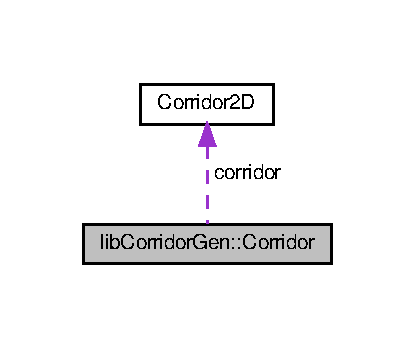
\includegraphics[width=199pt]{classlib_corridor_gen_1_1_corridor__coll__graph}
\end{center}
\end{figure}
\subsection*{Public Member Functions}
\begin{DoxyCompactItemize}
\item 
\hyperlink{classlib_corridor_gen_1_1_corridor_aeed77ae6b1e91f67df1d5f0d05de9f72}{Corridor} (std\+::shared\+\_\+ptr$<$ \hyperlink{classlib_corridor_gen_1_1_init_traj_planner}{Init\+Traj\+Planner} $>$ \+\_\+init\+Traj\+Planner\+\_\+obj, std\+::shared\+\_\+ptr$<$ octomap\+::\+Oc\+Tree $>$ \+\_\+octomap\+\_\+obj, \hyperlink{classlib_corridor_gen_1_1_param}{Param} \+\_\+param)
\item 
bool \hyperlink{classlib_corridor_gen_1_1_corridor_ac909b465688a8a5e50c6740f20c1b8bd}{update} (bool log)
\end{DoxyCompactItemize}
\subsection*{Public Attributes}
\begin{DoxyCompactItemize}
\item 
\hyperlink{struct_corridor2_d}{Corridor2D} \hyperlink{classlib_corridor_gen_1_1_corridor_af32ca65c896d5c952655106b74ea4666}{corridor}
\end{DoxyCompactItemize}


\subsection{Detailed Description}


Definition at line 20 of file corridor.\+hpp.



\subsection{Constructor \& Destructor Documentation}
\mbox{\Hypertarget{classlib_corridor_gen_1_1_corridor_aeed77ae6b1e91f67df1d5f0d05de9f72}\label{classlib_corridor_gen_1_1_corridor_aeed77ae6b1e91f67df1d5f0d05de9f72}} 
\index{lib\+Corridor\+Gen\+::\+Corridor@{lib\+Corridor\+Gen\+::\+Corridor}!Corridor@{Corridor}}
\index{Corridor@{Corridor}!lib\+Corridor\+Gen\+::\+Corridor@{lib\+Corridor\+Gen\+::\+Corridor}}
\subsubsection{\texorpdfstring{Corridor()}{Corridor()}}
{\footnotesize\ttfamily lib\+Corridor\+Gen\+::\+Corridor\+::\+Corridor (\begin{DoxyParamCaption}\item[{std\+::shared\+\_\+ptr$<$ \hyperlink{classlib_corridor_gen_1_1_init_traj_planner}{Init\+Traj\+Planner} $>$}]{\+\_\+init\+Traj\+Planner\+\_\+obj,  }\item[{std\+::shared\+\_\+ptr$<$ octomap\+::\+Oc\+Tree $>$}]{\+\_\+octomap\+\_\+obj,  }\item[{\hyperlink{classlib_corridor_gen_1_1_param}{Param}}]{\+\_\+param }\end{DoxyParamCaption})\hspace{0.3cm}{\ttfamily [inline]}}



Definition at line 24 of file corridor.\+hpp.



\subsection{Member Function Documentation}
\mbox{\Hypertarget{classlib_corridor_gen_1_1_corridor_ac909b465688a8a5e50c6740f20c1b8bd}\label{classlib_corridor_gen_1_1_corridor_ac909b465688a8a5e50c6740f20c1b8bd}} 
\index{lib\+Corridor\+Gen\+::\+Corridor@{lib\+Corridor\+Gen\+::\+Corridor}!update@{update}}
\index{update@{update}!lib\+Corridor\+Gen\+::\+Corridor@{lib\+Corridor\+Gen\+::\+Corridor}}
\subsubsection{\texorpdfstring{update()}{update()}}
{\footnotesize\ttfamily bool lib\+Corridor\+Gen\+::\+Corridor\+::update (\begin{DoxyParamCaption}\item[{bool}]{log }\end{DoxyParamCaption})\hspace{0.3cm}{\ttfamily [inline]}}



Definition at line 35 of file corridor.\+hpp.

Here is the call graph for this function\+:
\nopagebreak
\begin{figure}[H]
\begin{center}
\leavevmode
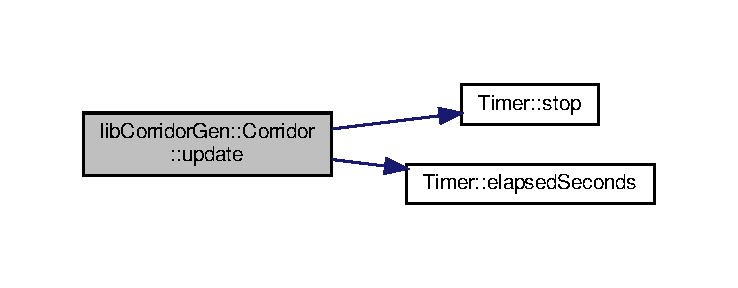
\includegraphics[width=350pt]{classlib_corridor_gen_1_1_corridor_ac909b465688a8a5e50c6740f20c1b8bd_cgraph}
\end{center}
\end{figure}


\subsection{Member Data Documentation}
\mbox{\Hypertarget{classlib_corridor_gen_1_1_corridor_af32ca65c896d5c952655106b74ea4666}\label{classlib_corridor_gen_1_1_corridor_af32ca65c896d5c952655106b74ea4666}} 
\index{lib\+Corridor\+Gen\+::\+Corridor@{lib\+Corridor\+Gen\+::\+Corridor}!corridor@{corridor}}
\index{corridor@{corridor}!lib\+Corridor\+Gen\+::\+Corridor@{lib\+Corridor\+Gen\+::\+Corridor}}
\subsubsection{\texorpdfstring{corridor}{corridor}}
{\footnotesize\ttfamily \hyperlink{struct_corridor2_d}{Corridor2D} lib\+Corridor\+Gen\+::\+Corridor\+::corridor}



Definition at line 22 of file corridor.\+hpp.



The documentation for this class was generated from the following file\+:\begin{DoxyCompactItemize}
\item 
include/\hyperlink{corridor_8hpp}{corridor.\+hpp}\end{DoxyCompactItemize}

\hypertarget{struct_corridor2_d}{}\section{Corridor2D Struct Reference}
\label{struct_corridor2_d}\index{Corridor2D@{Corridor2D}}


{\ttfamily \#include $<$corridor\+\_\+common.\+hpp$>$}

\subsection*{Public Member Functions}
\begin{DoxyCompactItemize}
\item 
\hyperlink{struct_corridor2_d_a7c7b0f2c9075543a29b39fdaa54f55c9}{Corridor2D} ()
\item 
\hyperlink{struct_corridor2_d_ae6b45a137b041daaf8a2c14f407d3891}{Corridor2D} (\hyperlink{corridor__common_8hpp_a14a6c0d0a5d79585147d5bab3bbb030a}{Box\+Constraint\+Seq} \hyperlink{struct_corridor2_d_a27a5f40ad109bda315a8bb67b517da28}{box\+\_\+seq}, \hyperlink{corridor__common_8hpp_a631ecdcd7d0a6bd15a6625fccbba7909}{Box\+Alloc\+Seq} \hyperlink{struct_corridor2_d_aa9eb677a900b8d7f875759e8f82d2b93}{box\+\_\+alloc\+\_\+seq}, double \hyperlink{struct_corridor2_d_a628834c7de6b20219858979b8ae5f3fa}{height})
\item 
std\+::vector$<$ geometry\+\_\+msgs\+::\+Point $>$ \hyperlink{struct_corridor2_d_a2b9a421e9f17340020bf16c286f4a246}{get\+\_\+corridor\+\_\+intersect\+\_\+points} ()
\item 
visualization\+\_\+msgs\+::\+Marker\+Array \hyperlink{struct_corridor2_d_a67ee02cbba27930d261fa313d2d83cc2}{get\+\_\+corridor\+\_\+markers} (std\+::string world\+\_\+frame\+\_\+id)
\end{DoxyCompactItemize}
\subsection*{Public Attributes}
\begin{DoxyCompactItemize}
\item 
\hyperlink{corridor__common_8hpp_a14a6c0d0a5d79585147d5bab3bbb030a}{Box\+Constraint\+Seq} \hyperlink{struct_corridor2_d_a27a5f40ad109bda315a8bb67b517da28}{box\+\_\+seq}
\item 
\hyperlink{corridor__common_8hpp_a631ecdcd7d0a6bd15a6625fccbba7909}{Box\+Alloc\+Seq} \hyperlink{struct_corridor2_d_aa9eb677a900b8d7f875759e8f82d2b93}{box\+\_\+alloc\+\_\+seq}
\item 
double \hyperlink{struct_corridor2_d_a628834c7de6b20219858979b8ae5f3fa}{height}
\end{DoxyCompactItemize}


\subsection{Detailed Description}


Definition at line 27 of file corridor\+\_\+common.\+hpp.



\subsection{Constructor \& Destructor Documentation}
\mbox{\Hypertarget{struct_corridor2_d_a7c7b0f2c9075543a29b39fdaa54f55c9}\label{struct_corridor2_d_a7c7b0f2c9075543a29b39fdaa54f55c9}} 
\index{Corridor2D@{Corridor2D}!Corridor2D@{Corridor2D}}
\index{Corridor2D@{Corridor2D}!Corridor2D@{Corridor2D}}
\subsubsection{\texorpdfstring{Corridor2\+D()}{Corridor2D()}\hspace{0.1cm}{\footnotesize\ttfamily [1/2]}}
{\footnotesize\ttfamily Corridor2\+D\+::\+Corridor2D (\begin{DoxyParamCaption}{ }\end{DoxyParamCaption})\hspace{0.3cm}{\ttfamily [inline]}}



Definition at line 31 of file corridor\+\_\+common.\+hpp.

\mbox{\Hypertarget{struct_corridor2_d_ae6b45a137b041daaf8a2c14f407d3891}\label{struct_corridor2_d_ae6b45a137b041daaf8a2c14f407d3891}} 
\index{Corridor2D@{Corridor2D}!Corridor2D@{Corridor2D}}
\index{Corridor2D@{Corridor2D}!Corridor2D@{Corridor2D}}
\subsubsection{\texorpdfstring{Corridor2\+D()}{Corridor2D()}\hspace{0.1cm}{\footnotesize\ttfamily [2/2]}}
{\footnotesize\ttfamily Corridor2\+D\+::\+Corridor2D (\begin{DoxyParamCaption}\item[{\hyperlink{corridor__common_8hpp_a14a6c0d0a5d79585147d5bab3bbb030a}{Box\+Constraint\+Seq}}]{box\+\_\+seq,  }\item[{\hyperlink{corridor__common_8hpp_a631ecdcd7d0a6bd15a6625fccbba7909}{Box\+Alloc\+Seq}}]{box\+\_\+alloc\+\_\+seq,  }\item[{double}]{height }\end{DoxyParamCaption})\hspace{0.3cm}{\ttfamily [inline]}}



Definition at line 32 of file corridor\+\_\+common.\+hpp.



\subsection{Member Function Documentation}
\mbox{\Hypertarget{struct_corridor2_d_a2b9a421e9f17340020bf16c286f4a246}\label{struct_corridor2_d_a2b9a421e9f17340020bf16c286f4a246}} 
\index{Corridor2D@{Corridor2D}!get\+\_\+corridor\+\_\+intersect\+\_\+points@{get\+\_\+corridor\+\_\+intersect\+\_\+points}}
\index{get\+\_\+corridor\+\_\+intersect\+\_\+points@{get\+\_\+corridor\+\_\+intersect\+\_\+points}!Corridor2D@{Corridor2D}}
\subsubsection{\texorpdfstring{get\+\_\+corridor\+\_\+intersect\+\_\+points()}{get\_corridor\_intersect\_points()}}
{\footnotesize\ttfamily std\+::vector$<$geometry\+\_\+msgs\+::\+Point$>$ Corridor2\+D\+::get\+\_\+corridor\+\_\+intersect\+\_\+points (\begin{DoxyParamCaption}{ }\end{DoxyParamCaption})}

\mbox{\Hypertarget{struct_corridor2_d_a67ee02cbba27930d261fa313d2d83cc2}\label{struct_corridor2_d_a67ee02cbba27930d261fa313d2d83cc2}} 
\index{Corridor2D@{Corridor2D}!get\+\_\+corridor\+\_\+markers@{get\+\_\+corridor\+\_\+markers}}
\index{get\+\_\+corridor\+\_\+markers@{get\+\_\+corridor\+\_\+markers}!Corridor2D@{Corridor2D}}
\subsubsection{\texorpdfstring{get\+\_\+corridor\+\_\+markers()}{get\_corridor\_markers()}}
{\footnotesize\ttfamily visualization\+\_\+msgs\+::\+Marker\+Array Corridor2\+D\+::get\+\_\+corridor\+\_\+markers (\begin{DoxyParamCaption}\item[{std\+::string}]{world\+\_\+frame\+\_\+id }\end{DoxyParamCaption})}



\subsection{Member Data Documentation}
\mbox{\Hypertarget{struct_corridor2_d_aa9eb677a900b8d7f875759e8f82d2b93}\label{struct_corridor2_d_aa9eb677a900b8d7f875759e8f82d2b93}} 
\index{Corridor2D@{Corridor2D}!box\+\_\+alloc\+\_\+seq@{box\+\_\+alloc\+\_\+seq}}
\index{box\+\_\+alloc\+\_\+seq@{box\+\_\+alloc\+\_\+seq}!Corridor2D@{Corridor2D}}
\subsubsection{\texorpdfstring{box\+\_\+alloc\+\_\+seq}{box\_alloc\_seq}}
{\footnotesize\ttfamily \hyperlink{corridor__common_8hpp_a631ecdcd7d0a6bd15a6625fccbba7909}{Box\+Alloc\+Seq} Corridor2\+D\+::box\+\_\+alloc\+\_\+seq}



Definition at line 29 of file corridor\+\_\+common.\+hpp.

\mbox{\Hypertarget{struct_corridor2_d_a27a5f40ad109bda315a8bb67b517da28}\label{struct_corridor2_d_a27a5f40ad109bda315a8bb67b517da28}} 
\index{Corridor2D@{Corridor2D}!box\+\_\+seq@{box\+\_\+seq}}
\index{box\+\_\+seq@{box\+\_\+seq}!Corridor2D@{Corridor2D}}
\subsubsection{\texorpdfstring{box\+\_\+seq}{box\_seq}}
{\footnotesize\ttfamily \hyperlink{corridor__common_8hpp_a14a6c0d0a5d79585147d5bab3bbb030a}{Box\+Constraint\+Seq} Corridor2\+D\+::box\+\_\+seq}



Definition at line 28 of file corridor\+\_\+common.\+hpp.

\mbox{\Hypertarget{struct_corridor2_d_a628834c7de6b20219858979b8ae5f3fa}\label{struct_corridor2_d_a628834c7de6b20219858979b8ae5f3fa}} 
\index{Corridor2D@{Corridor2D}!height@{height}}
\index{height@{height}!Corridor2D@{Corridor2D}}
\subsubsection{\texorpdfstring{height}{height}}
{\footnotesize\ttfamily double Corridor2\+D\+::height}



Definition at line 30 of file corridor\+\_\+common.\+hpp.



The documentation for this struct was generated from the following file\+:\begin{DoxyCompactItemize}
\item 
include/\hyperlink{corridor__common_8hpp}{corridor\+\_\+common.\+hpp}\end{DoxyCompactItemize}

\hypertarget{classlib_multi_robot_planning_1_1_e_c_b_s}{}\section{lib\+Multi\+Robot\+Planning\+:\+:E\+C\+BS$<$ State, Action, Cost, Conflict, Constraints, Environment $>$ Class Template Reference}
\label{classlib_multi_robot_planning_1_1_e_c_b_s}\index{lib\+Multi\+Robot\+Planning\+::\+E\+C\+B\+S$<$ State, Action, Cost, Conflict, Constraints, Environment $>$@{lib\+Multi\+Robot\+Planning\+::\+E\+C\+B\+S$<$ State, Action, Cost, Conflict, Constraints, Environment $>$}}


Enhanced Conflict-\/\+Based-\/\+Search (\hyperlink{classlib_multi_robot_planning_1_1_e_c_b_s}{E\+C\+BS}) algorithm to solve the Multi-\/\+Agent Path-\/\+Finding (M\+A\+PF) problem within a given suboptimality bound.  




{\ttfamily \#include $<$ecbs.\+hpp$>$}

\subsection*{Public Member Functions}
\begin{DoxyCompactItemize}
\item 
\hyperlink{classlib_multi_robot_planning_1_1_e_c_b_s_acfa9763a8d2a9bbf76736343e266a419}{E\+C\+BS} (\hyperlink{classlib_multi_robot_planning_1_1_environment}{Environment} \&environment, float w)
\item 
bool \hyperlink{classlib_multi_robot_planning_1_1_e_c_b_s_afecd0fb22e9070ee79391a6850c15f3d}{search} (const std\+::vector$<$ \hyperlink{structlib_multi_robot_planning_1_1_state}{State} $>$ \&initial\+States, std\+::vector$<$ \hyperlink{structlib_multi_robot_planning_1_1_plan_result}{Plan\+Result}$<$ \hyperlink{structlib_multi_robot_planning_1_1_state}{State}, \hyperlink{namespacelib_multi_robot_planning_aba73fb71693f86a324adfa0e41e1053d}{Action}, Cost $>$ $>$ \&solution)
\end{DoxyCompactItemize}


\subsection{Detailed Description}
\subsubsection*{template$<$typename State, typename Action, typename Cost, typename Conflict, typename Constraints, typename Environment$>$\newline
class lib\+Multi\+Robot\+Planning\+::\+E\+C\+B\+S$<$ State, Action, Cost, Conflict, Constraints, Environment $>$}

Enhanced Conflict-\/\+Based-\/\+Search (\hyperlink{classlib_multi_robot_planning_1_1_e_c_b_s}{E\+C\+BS}) algorithm to solve the Multi-\/\+Agent Path-\/\+Finding (M\+A\+PF) problem within a given suboptimality bound. 

This class implements the Enhanced Conflict-\/\+Based-\/\+Search (\hyperlink{classlib_multi_robot_planning_1_1_e_c_b_s}{E\+C\+BS}) algorithm. This algorithm can find collision-\/free path for multiple agents with start and goal locations given for each agent. A user can provide a suboptimality factor w, and the cost of the returned solution is guaranteed to smaller or equal than w $\ast$ optimal\+Cost. \hyperlink{classlib_multi_robot_planning_1_1_e_c_b_s}{E\+C\+BS} is an extension of \hyperlink{classlib_multi_robot_planning_1_1_c_b_s}{C\+BS}. It uses the same two-\/level search with a focal search on both levels. The focal search uses a second user-\/provided inadmissible heuristic that minimizes conflicts between agents.

Details of the algorithm can be found in the following paper\+:~\newline
Max Barer, Guni Sharon, Roni Stern, Ariel Felner\+:~\newline
\char`\"{}\+Suboptimal Variants of the Conflict-\/\+Based Search Algorithm for the Multi-\/\+Agent
\+Pathfinding Problem\char`\"{}. S\+O\+CS 2014~\newline
\href{http://www.aaai.org/ocs/index.php/SOCS/SOCS14/paper/view/8911}{\tt http\+://www.\+aaai.\+org/ocs/index.\+php/\+S\+O\+C\+S/\+S\+O\+C\+S14/paper/view/8911}

The underlying A$\ast$\+\_\+epsilon algorithm can either use a fibonacci heap, or a d-\/ary heap. The latter is the default. Define \char`\"{}\+U\+S\+E\+\_\+\+F\+I\+B\+O\+N\+A\+C\+C\+I\+\_\+\+H\+E\+A\+P\char`\"{} to use the fibonacci heap instead.


\begin{DoxyTemplParams}{Template Parameters}
{\em \hyperlink{structlib_multi_robot_planning_1_1_state}{State}} & Custom state for the search. Needs to be copy\textquotesingle{}able \\
\hline
{\em Action} & Custom action for the search. Needs to be copy\textquotesingle{}able \\
\hline
{\em Cost} & Custom Cost type (integer or floating point types) \\
\hline
{\em \hyperlink{structlib_multi_robot_planning_1_1_conflict}{Conflict}} & Custom conflict description. A conflict needs to be able to be transformed into a constraint. \\
\hline
{\em \hyperlink{structlib_multi_robot_planning_1_1_constraints}{Constraints}} & Custom constraint description. The \hyperlink{classlib_multi_robot_planning_1_1_environment}{Environment} needs to be able to search on the low-\/level while taking the constraints into account. \\
\hline
{\em \hyperlink{classlib_multi_robot_planning_1_1_environment}{Environment}} & This class needs to provide the custom logic. In particular, it needs to support the following functions\+:
\begin{DoxyItemize}
\item {\ttfamily void set\+Low\+Level\+Context(size\+\_\+t agent\+Idx, const Constraints$\ast$ constraints)}~\newline
 Set the current context to a particular agent with the given set of constraints
\item {\ttfamily Cost admissible\+Heuristic(const State\& s)}~\newline
 Admissible heuristic. Needs to take current context into account.
\item {\ttfamily Cost focal\+State\+Heuristic(const \hyperlink{structlib_multi_robot_planning_1_1_state}{State}\& s, int g\+Score, const std\+::vector$<$\hyperlink{structlib_multi_robot_planning_1_1_plan_result}{Plan\+Result}$<$\hyperlink{structlib_multi_robot_planning_1_1_state}{State}, Action, int$>$ $>$\& solution)}~\newline
 Potentially inadmissible focal heuristic for a state, e.\+g. count all conflicts between the agents if the agent of the current context moves is at state s
\item `\+Cost focal\+Transition\+Heuristic(const \hyperlink{structlib_multi_robot_planning_1_1_state}{State}\& s1a, const \hyperlink{structlib_multi_robot_planning_1_1_state}{State}\& s1b, Cost g\+Score\+S1a, Cost g\+Score\+S1b, const std\+::vector$<$Plan\+Result$<$\+State, Action, Cost$>$ $>$\& solution)`~\newline
 Potentially inadmissible focal heuristic for a state transition, e.\+g. count all conflicts between the agents if the agent of the current context moves from s1a to s1b
\item {\ttfamily Cost focal\+Heuristic(const std\+::vector$<$\hyperlink{structlib_multi_robot_planning_1_1_plan_result}{Plan\+Result}$<$\hyperlink{structlib_multi_robot_planning_1_1_state}{State}, Action, int$>$ $>$\& solution)}~\newline
 Potentially inadmissible focal heuristic, e.\+g. count all conflicts between the agents for a given solution
\item {\ttfamily bool is\+Solution(const State\& s)}~\newline
 Return true if the given state is a goal state for the current agent.
\item {\ttfamily void get\+Neighbors(const \hyperlink{structlib_multi_robot_planning_1_1_state}{State}\& s, std\+::vector$<$\hyperlink{structlib_multi_robot_planning_1_1_neighbor}{Neighbor}$<$\hyperlink{structlib_multi_robot_planning_1_1_state}{State}, Action, int$>$ $>$\& neighbors)}~\newline
 Fill the list of neighboring state for the given state s and the current agent.
\item {\ttfamily bool get\+First\+Conflict(const std\+::vector$<$\hyperlink{structlib_multi_robot_planning_1_1_plan_result}{Plan\+Result}$<$\hyperlink{structlib_multi_robot_planning_1_1_state}{State}, Action, int$>$ $>$\& solution, \hyperlink{structlib_multi_robot_planning_1_1_conflict}{Conflict}\& result)}~\newline
 Finds the first conflict for the given solution for each agent. Return true if a conflict was found and false otherwise.
\item {\ttfamily void create\+Constraints\+From\+Conflict(const \hyperlink{structlib_multi_robot_planning_1_1_conflict}{Conflict}\& conflict, std\+::map$<$size\+\_\+t, \hyperlink{structlib_multi_robot_planning_1_1_constraints}{Constraints}$>$\& constraints)}~\newline
 Create a list of constraints for the given conflict.
\item {\ttfamily void on\+Expand\+High\+Level\+Node(\+Cost cost)}~\newline
 This function is called on every high-\/level expansion and can be used for statistical purposes.
\item {\ttfamily void on\+Expand\+Low\+Level\+Node(const State\& s, Cost f\+Score, Cost g\+Score)}~\newline
 This function is called on every low-\/level expansion and can be used for statistical purposes.
\end{DoxyItemize}\\
\hline
\end{DoxyTemplParams}
\begin{DoxySeeAlso}{See also}
\hyperlink{classlib_multi_robot_planning_1_1_c_b_s}{C\+BS} 
\end{DoxySeeAlso}


Definition at line 105 of file ecbs.\+hpp.



\subsection{Constructor \& Destructor Documentation}
\mbox{\Hypertarget{classlib_multi_robot_planning_1_1_e_c_b_s_acfa9763a8d2a9bbf76736343e266a419}\label{classlib_multi_robot_planning_1_1_e_c_b_s_acfa9763a8d2a9bbf76736343e266a419}} 
\index{lib\+Multi\+Robot\+Planning\+::\+E\+C\+BS@{lib\+Multi\+Robot\+Planning\+::\+E\+C\+BS}!E\+C\+BS@{E\+C\+BS}}
\index{E\+C\+BS@{E\+C\+BS}!lib\+Multi\+Robot\+Planning\+::\+E\+C\+BS@{lib\+Multi\+Robot\+Planning\+::\+E\+C\+BS}}
\subsubsection{\texorpdfstring{E\+C\+B\+S()}{ECBS()}}
{\footnotesize\ttfamily template$<$typename State, typename Action, typename Cost, typename Conflict, typename Constraints, typename Environment$>$ \\
\hyperlink{classlib_multi_robot_planning_1_1_e_c_b_s}{lib\+Multi\+Robot\+Planning\+::\+E\+C\+BS}$<$ \hyperlink{structlib_multi_robot_planning_1_1_state}{State}, \hyperlink{namespacelib_multi_robot_planning_aba73fb71693f86a324adfa0e41e1053d}{Action}, Cost, \hyperlink{structlib_multi_robot_planning_1_1_conflict}{Conflict}, \hyperlink{structlib_multi_robot_planning_1_1_constraints}{Constraints}, \hyperlink{classlib_multi_robot_planning_1_1_environment}{Environment} $>$\+::\hyperlink{classlib_multi_robot_planning_1_1_e_c_b_s}{E\+C\+BS} (\begin{DoxyParamCaption}\item[{\hyperlink{classlib_multi_robot_planning_1_1_environment}{Environment} \&}]{environment,  }\item[{float}]{w }\end{DoxyParamCaption})\hspace{0.3cm}{\ttfamily [inline]}}



Definition at line 107 of file ecbs.\+hpp.



\subsection{Member Function Documentation}
\mbox{\Hypertarget{classlib_multi_robot_planning_1_1_e_c_b_s_afecd0fb22e9070ee79391a6850c15f3d}\label{classlib_multi_robot_planning_1_1_e_c_b_s_afecd0fb22e9070ee79391a6850c15f3d}} 
\index{lib\+Multi\+Robot\+Planning\+::\+E\+C\+BS@{lib\+Multi\+Robot\+Planning\+::\+E\+C\+BS}!search@{search}}
\index{search@{search}!lib\+Multi\+Robot\+Planning\+::\+E\+C\+BS@{lib\+Multi\+Robot\+Planning\+::\+E\+C\+BS}}
\subsubsection{\texorpdfstring{search()}{search()}}
{\footnotesize\ttfamily template$<$typename State, typename Action, typename Cost, typename Conflict, typename Constraints, typename Environment$>$ \\
bool \hyperlink{classlib_multi_robot_planning_1_1_e_c_b_s}{lib\+Multi\+Robot\+Planning\+::\+E\+C\+BS}$<$ \hyperlink{structlib_multi_robot_planning_1_1_state}{State}, \hyperlink{namespacelib_multi_robot_planning_aba73fb71693f86a324adfa0e41e1053d}{Action}, Cost, \hyperlink{structlib_multi_robot_planning_1_1_conflict}{Conflict}, \hyperlink{structlib_multi_robot_planning_1_1_constraints}{Constraints}, \hyperlink{classlib_multi_robot_planning_1_1_environment}{Environment} $>$\+::search (\begin{DoxyParamCaption}\item[{const std\+::vector$<$ \hyperlink{structlib_multi_robot_planning_1_1_state}{State} $>$ \&}]{initial\+States,  }\item[{std\+::vector$<$ \hyperlink{structlib_multi_robot_planning_1_1_plan_result}{Plan\+Result}$<$ \hyperlink{structlib_multi_robot_planning_1_1_state}{State}, \hyperlink{namespacelib_multi_robot_planning_aba73fb71693f86a324adfa0e41e1053d}{Action}, Cost $>$ $>$ \&}]{solution }\end{DoxyParamCaption})\hspace{0.3cm}{\ttfamily [inline]}}



Definition at line 109 of file ecbs.\+hpp.

Here is the call graph for this function\+:
\nopagebreak
\begin{figure}[H]
\begin{center}
\leavevmode
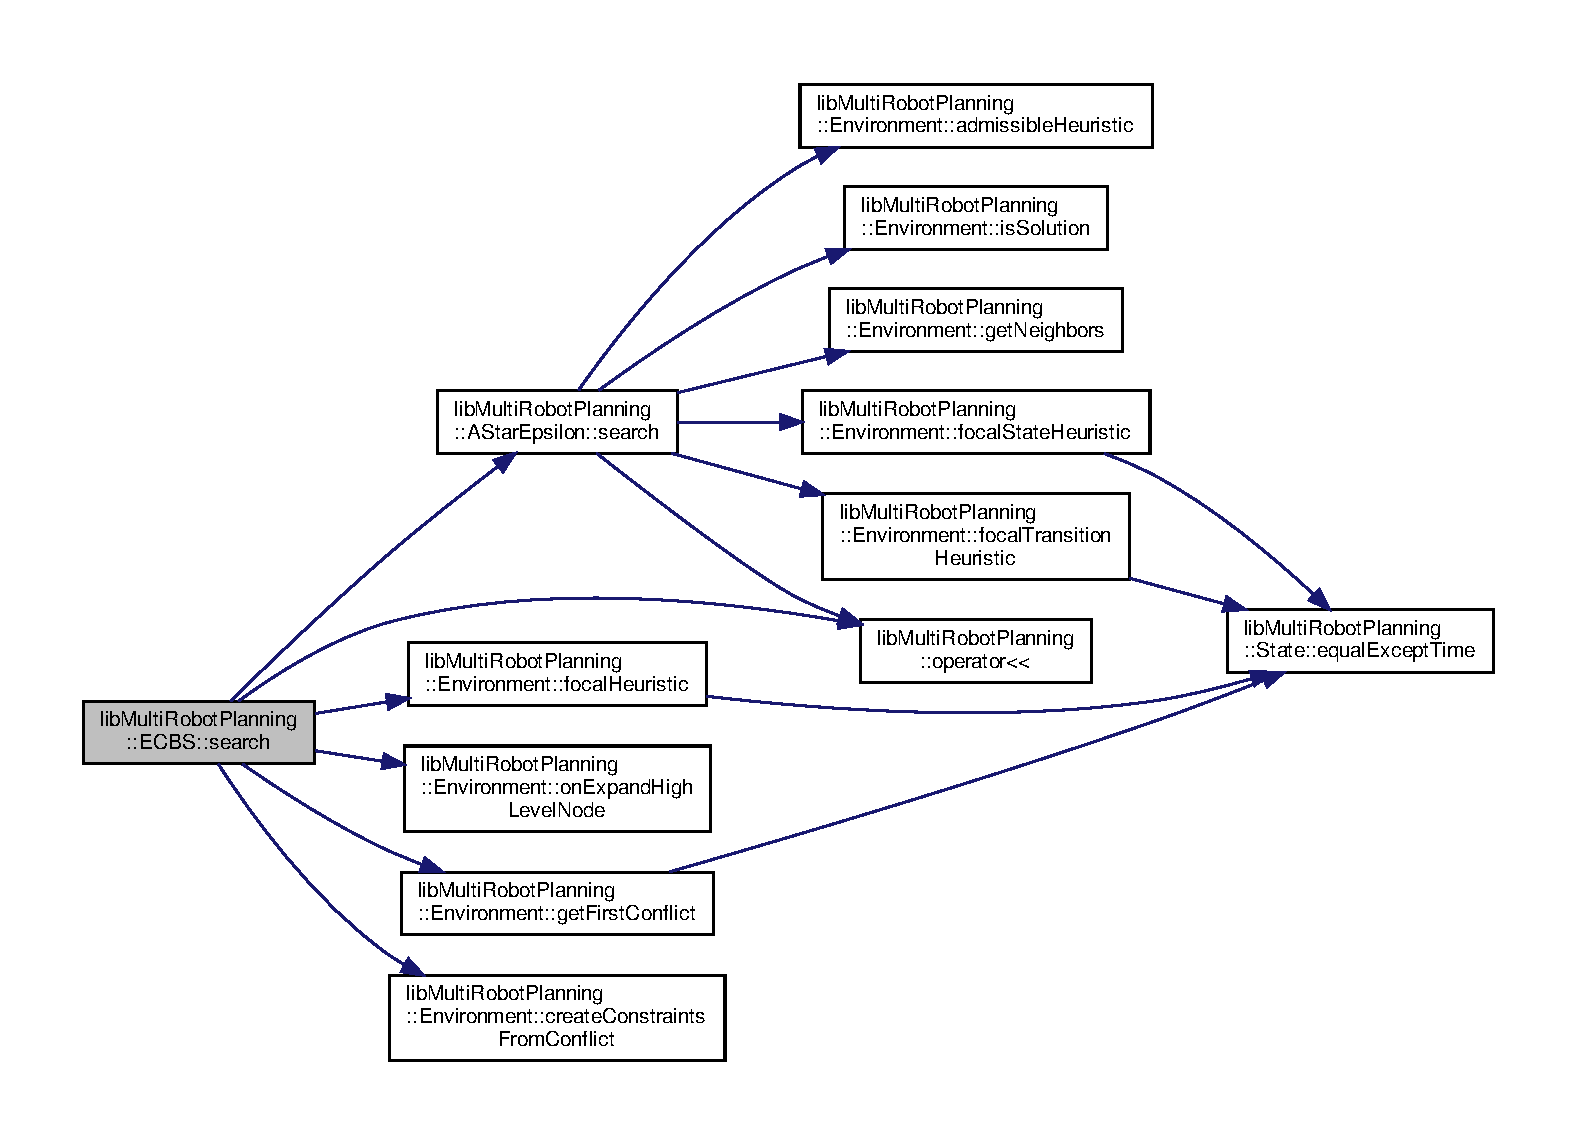
\includegraphics[width=350pt]{classlib_multi_robot_planning_1_1_e_c_b_s_afecd0fb22e9070ee79391a6850c15f3d_cgraph}
\end{center}
\end{figure}
Here is the caller graph for this function\+:
\nopagebreak
\begin{figure}[H]
\begin{center}
\leavevmode
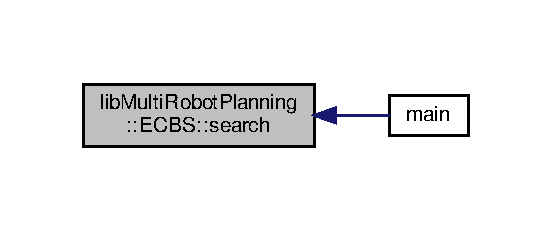
\includegraphics[width=265pt]{classlib_multi_robot_planning_1_1_e_c_b_s_afecd0fb22e9070ee79391a6850c15f3d_icgraph}
\end{center}
\end{figure}


The documentation for this class was generated from the following file\+:\begin{DoxyCompactItemize}
\item 
third\+\_\+party/ecbs/include/\hyperlink{ecbs_8hpp}{ecbs.\+hpp}\end{DoxyCompactItemize}

\hypertarget{classlib_corridor_gen_1_1_e_c_b_s_planner}{}\section{lib\+Corridor\+Gen\+:\+:E\+C\+B\+S\+Planner Class Reference}
\label{classlib_corridor_gen_1_1_e_c_b_s_planner}\index{lib\+Corridor\+Gen\+::\+E\+C\+B\+S\+Planner@{lib\+Corridor\+Gen\+::\+E\+C\+B\+S\+Planner}}


{\ttfamily \#include $<$ecbs\+\_\+planner.\+hpp$>$}



Inheritance diagram for lib\+Corridor\+Gen\+:\+:E\+C\+B\+S\+Planner\+:
\nopagebreak
\begin{figure}[H]
\begin{center}
\leavevmode
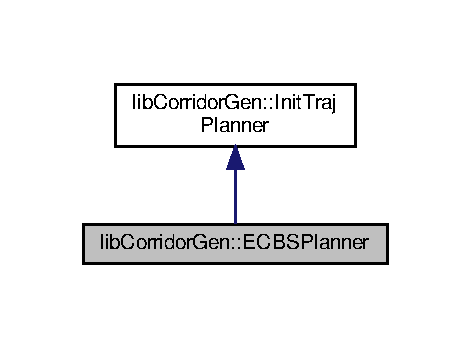
\includegraphics[width=226pt]{classlib_corridor_gen_1_1_e_c_b_s_planner__inherit__graph}
\end{center}
\end{figure}


Collaboration diagram for lib\+Corridor\+Gen\+:\+:E\+C\+B\+S\+Planner\+:
\nopagebreak
\begin{figure}[H]
\begin{center}
\leavevmode
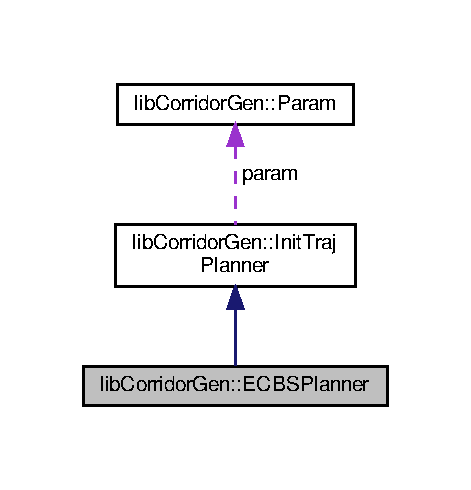
\includegraphics[width=226pt]{classlib_corridor_gen_1_1_e_c_b_s_planner__coll__graph}
\end{center}
\end{figure}
\subsection*{Public Member Functions}
\begin{DoxyCompactItemize}
\item 
\hyperlink{classlib_corridor_gen_1_1_e_c_b_s_planner_af300eb5080e7979bef2f62d8886f5c85}{E\+C\+B\+S\+Planner} (std\+::shared\+\_\+ptr$<$ octomap\+::\+Oc\+Tree $>$ \+\_\+octree\+\_\+obj, \hyperlink{classlib_corridor_gen_1_1_param}{Param} \+\_\+param)
\item 
bool \hyperlink{classlib_corridor_gen_1_1_e_c_b_s_planner_a0d4c5855c02228c677b3d2d89c10740c}{update} (bool log) override
\end{DoxyCompactItemize}
\subsection*{Additional Inherited Members}


\subsection{Detailed Description}


Definition at line 9 of file ecbs\+\_\+planner.\+hpp.



\subsection{Constructor \& Destructor Documentation}
\mbox{\Hypertarget{classlib_corridor_gen_1_1_e_c_b_s_planner_af300eb5080e7979bef2f62d8886f5c85}\label{classlib_corridor_gen_1_1_e_c_b_s_planner_af300eb5080e7979bef2f62d8886f5c85}} 
\index{lib\+Corridor\+Gen\+::\+E\+C\+B\+S\+Planner@{lib\+Corridor\+Gen\+::\+E\+C\+B\+S\+Planner}!E\+C\+B\+S\+Planner@{E\+C\+B\+S\+Planner}}
\index{E\+C\+B\+S\+Planner@{E\+C\+B\+S\+Planner}!lib\+Corridor\+Gen\+::\+E\+C\+B\+S\+Planner@{lib\+Corridor\+Gen\+::\+E\+C\+B\+S\+Planner}}
\subsubsection{\texorpdfstring{E\+C\+B\+S\+Planner()}{ECBSPlanner()}}
{\footnotesize\ttfamily lib\+Corridor\+Gen\+::\+E\+C\+B\+S\+Planner\+::\+E\+C\+B\+S\+Planner (\begin{DoxyParamCaption}\item[{std\+::shared\+\_\+ptr$<$ octomap\+::\+Oc\+Tree $>$}]{\+\_\+octree\+\_\+obj,  }\item[{\hyperlink{classlib_corridor_gen_1_1_param}{Param}}]{\+\_\+param }\end{DoxyParamCaption})\hspace{0.3cm}{\ttfamily [inline]}}



Definition at line 11 of file ecbs\+\_\+planner.\+hpp.



\subsection{Member Function Documentation}
\mbox{\Hypertarget{classlib_corridor_gen_1_1_e_c_b_s_planner_a0d4c5855c02228c677b3d2d89c10740c}\label{classlib_corridor_gen_1_1_e_c_b_s_planner_a0d4c5855c02228c677b3d2d89c10740c}} 
\index{lib\+Corridor\+Gen\+::\+E\+C\+B\+S\+Planner@{lib\+Corridor\+Gen\+::\+E\+C\+B\+S\+Planner}!update@{update}}
\index{update@{update}!lib\+Corridor\+Gen\+::\+E\+C\+B\+S\+Planner@{lib\+Corridor\+Gen\+::\+E\+C\+B\+S\+Planner}}
\subsubsection{\texorpdfstring{update()}{update()}}
{\footnotesize\ttfamily bool lib\+Corridor\+Gen\+::\+E\+C\+B\+S\+Planner\+::update (\begin{DoxyParamCaption}\item[{bool}]{log }\end{DoxyParamCaption})\hspace{0.3cm}{\ttfamily [inline]}, {\ttfamily [override]}, {\ttfamily [virtual]}}



Implements \hyperlink{classlib_corridor_gen_1_1_init_traj_planner_acfc10a68eddb236a10790c4d92473d99}{lib\+Corridor\+Gen\+::\+Init\+Traj\+Planner}.



Definition at line 19 of file ecbs\+\_\+planner.\+hpp.



The documentation for this class was generated from the following file\+:\begin{DoxyCompactItemize}
\item 
include/\hyperlink{ecbs__planner_8hpp}{ecbs\+\_\+planner.\+hpp}\end{DoxyCompactItemize}

\hypertarget{struct_edge_constraint}{}\section{Edge\+Constraint Struct Reference}
\label{struct_edge_constraint}\index{Edge\+Constraint@{Edge\+Constraint}}
\subsection*{Public Member Functions}
\begin{DoxyCompactItemize}
\item 
\hyperlink{struct_edge_constraint_a9a9f97acb89f2086589a058d8ea10cf8}{Edge\+Constraint} (int \hyperlink{struct_edge_constraint_aa4a694babdcc422c4914ec768994119b}{time}, int \hyperlink{struct_edge_constraint_a71519eb54d966deeed3ac62bfabb6248}{x1}, int \hyperlink{struct_edge_constraint_ada1765ae9a023f4725d515410854efe4}{y1}, int \hyperlink{struct_edge_constraint_aef17564b45f61b8d1112b26fcb2530cc}{z1}, int \hyperlink{struct_edge_constraint_ac586d7c34a6aa83734a860390b99b011}{x2}, int \hyperlink{struct_edge_constraint_a4575744b1bc5386c9195074e73586e96}{y2}, int \hyperlink{struct_edge_constraint_a11aa005fe0bd29b4bf4da5e0429dcba6}{z2})
\item 
bool \hyperlink{struct_edge_constraint_ab34ad90076811f3480434e7446c5c07a}{operator$<$} (const \hyperlink{struct_edge_constraint}{Edge\+Constraint} \&other) const
\item 
bool \hyperlink{struct_edge_constraint_a0bb713ad9bf7afb42e84d85a94656af0}{operator==} (const \hyperlink{struct_edge_constraint}{Edge\+Constraint} \&other) const
\item 
\hyperlink{struct_edge_constraint_a752ce9d7097739927ba5edcd25f617a7}{Edge\+Constraint} (int \hyperlink{struct_edge_constraint_aa4a694babdcc422c4914ec768994119b}{time}, int \hyperlink{struct_edge_constraint_a71519eb54d966deeed3ac62bfabb6248}{x1}, int \hyperlink{struct_edge_constraint_ada1765ae9a023f4725d515410854efe4}{y1}, int \hyperlink{struct_edge_constraint_ac586d7c34a6aa83734a860390b99b011}{x2}, int \hyperlink{struct_edge_constraint_a4575744b1bc5386c9195074e73586e96}{y2}, int \hyperlink{struct_edge_constraint_aef17564b45f61b8d1112b26fcb2530cc}{z1}, int \hyperlink{struct_edge_constraint_a11aa005fe0bd29b4bf4da5e0429dcba6}{z2})
\item 
bool \hyperlink{struct_edge_constraint_ab34ad90076811f3480434e7446c5c07a}{operator$<$} (const \hyperlink{struct_edge_constraint}{Edge\+Constraint} \&other) const
\item 
bool \hyperlink{struct_edge_constraint_a0bb713ad9bf7afb42e84d85a94656af0}{operator==} (const \hyperlink{struct_edge_constraint}{Edge\+Constraint} \&other) const
\end{DoxyCompactItemize}
\subsection*{Public Attributes}
\begin{DoxyCompactItemize}
\item 
int \hyperlink{struct_edge_constraint_aa4a694babdcc422c4914ec768994119b}{time}
\item 
int \hyperlink{struct_edge_constraint_a71519eb54d966deeed3ac62bfabb6248}{x1}
\item 
int \hyperlink{struct_edge_constraint_ada1765ae9a023f4725d515410854efe4}{y1}
\item 
int \hyperlink{struct_edge_constraint_aef17564b45f61b8d1112b26fcb2530cc}{z1}
\item 
int \hyperlink{struct_edge_constraint_ac586d7c34a6aa83734a860390b99b011}{x2}
\item 
int \hyperlink{struct_edge_constraint_a4575744b1bc5386c9195074e73586e96}{y2}
\item 
int \hyperlink{struct_edge_constraint_a11aa005fe0bd29b4bf4da5e0429dcba6}{z2}
\end{DoxyCompactItemize}
\subsection*{Friends}
\begin{DoxyCompactItemize}
\item 
std\+::ostream \& \hyperlink{struct_edge_constraint_a94c3e6e61fef6fe98974b7bcf1b2245e}{operator$<$$<$} (std\+::ostream \&os, const \hyperlink{struct_edge_constraint}{Edge\+Constraint} \&c)
\item 
std\+::ostream \& \hyperlink{struct_edge_constraint_a94c3e6e61fef6fe98974b7bcf1b2245e}{operator$<$$<$} (std\+::ostream \&os, const \hyperlink{struct_edge_constraint}{Edge\+Constraint} \&c)
\end{DoxyCompactItemize}


\subsection{Detailed Description}


Definition at line 154 of file cbs.\+cpp.



\subsection{Constructor \& Destructor Documentation}
\mbox{\Hypertarget{struct_edge_constraint_a9a9f97acb89f2086589a058d8ea10cf8}\label{struct_edge_constraint_a9a9f97acb89f2086589a058d8ea10cf8}} 
\index{Edge\+Constraint@{Edge\+Constraint}!Edge\+Constraint@{Edge\+Constraint}}
\index{Edge\+Constraint@{Edge\+Constraint}!Edge\+Constraint@{Edge\+Constraint}}
\subsubsection{\texorpdfstring{Edge\+Constraint()}{EdgeConstraint()}\hspace{0.1cm}{\footnotesize\ttfamily [1/2]}}
{\footnotesize\ttfamily Edge\+Constraint\+::\+Edge\+Constraint (\begin{DoxyParamCaption}\item[{int}]{time,  }\item[{int}]{x1,  }\item[{int}]{y1,  }\item[{int}]{z1,  }\item[{int}]{x2,  }\item[{int}]{y2,  }\item[{int}]{z2 }\end{DoxyParamCaption})\hspace{0.3cm}{\ttfamily [inline]}}



Definition at line 155 of file cbs.\+cpp.

\mbox{\Hypertarget{struct_edge_constraint_a752ce9d7097739927ba5edcd25f617a7}\label{struct_edge_constraint_a752ce9d7097739927ba5edcd25f617a7}} 
\index{Edge\+Constraint@{Edge\+Constraint}!Edge\+Constraint@{Edge\+Constraint}}
\index{Edge\+Constraint@{Edge\+Constraint}!Edge\+Constraint@{Edge\+Constraint}}
\subsubsection{\texorpdfstring{Edge\+Constraint()}{EdgeConstraint()}\hspace{0.1cm}{\footnotesize\ttfamily [2/2]}}
{\footnotesize\ttfamily Edge\+Constraint\+::\+Edge\+Constraint (\begin{DoxyParamCaption}\item[{int}]{time,  }\item[{int}]{x1,  }\item[{int}]{y1,  }\item[{int}]{x2,  }\item[{int}]{y2,  }\item[{int}]{z1,  }\item[{int}]{z2 }\end{DoxyParamCaption})\hspace{0.3cm}{\ttfamily [inline]}}



Definition at line 155 of file ecbs.\+cpp.



\subsection{Member Function Documentation}
\mbox{\Hypertarget{struct_edge_constraint_ab34ad90076811f3480434e7446c5c07a}\label{struct_edge_constraint_ab34ad90076811f3480434e7446c5c07a}} 
\index{Edge\+Constraint@{Edge\+Constraint}!operator$<$@{operator$<$}}
\index{operator$<$@{operator$<$}!Edge\+Constraint@{Edge\+Constraint}}
\subsubsection{\texorpdfstring{operator$<$()}{operator<()}\hspace{0.1cm}{\footnotesize\ttfamily [1/2]}}
{\footnotesize\ttfamily bool Edge\+Constraint\+::operator$<$ (\begin{DoxyParamCaption}\item[{const \hyperlink{struct_edge_constraint}{Edge\+Constraint} \&}]{other }\end{DoxyParamCaption}) const\hspace{0.3cm}{\ttfamily [inline]}}



Definition at line 165 of file cbs.\+cpp.

\mbox{\Hypertarget{struct_edge_constraint_ab34ad90076811f3480434e7446c5c07a}\label{struct_edge_constraint_ab34ad90076811f3480434e7446c5c07a}} 
\index{Edge\+Constraint@{Edge\+Constraint}!operator$<$@{operator$<$}}
\index{operator$<$@{operator$<$}!Edge\+Constraint@{Edge\+Constraint}}
\subsubsection{\texorpdfstring{operator$<$()}{operator<()}\hspace{0.1cm}{\footnotesize\ttfamily [2/2]}}
{\footnotesize\ttfamily bool Edge\+Constraint\+::operator$<$ (\begin{DoxyParamCaption}\item[{const \hyperlink{struct_edge_constraint}{Edge\+Constraint} \&}]{other }\end{DoxyParamCaption}) const\hspace{0.3cm}{\ttfamily [inline]}}



Definition at line 165 of file ecbs.\+cpp.

\mbox{\Hypertarget{struct_edge_constraint_a0bb713ad9bf7afb42e84d85a94656af0}\label{struct_edge_constraint_a0bb713ad9bf7afb42e84d85a94656af0}} 
\index{Edge\+Constraint@{Edge\+Constraint}!operator==@{operator==}}
\index{operator==@{operator==}!Edge\+Constraint@{Edge\+Constraint}}
\subsubsection{\texorpdfstring{operator==()}{operator==()}\hspace{0.1cm}{\footnotesize\ttfamily [1/2]}}
{\footnotesize\ttfamily bool Edge\+Constraint\+::operator== (\begin{DoxyParamCaption}\item[{const \hyperlink{struct_edge_constraint}{Edge\+Constraint} \&}]{other }\end{DoxyParamCaption}) const\hspace{0.3cm}{\ttfamily [inline]}}



Definition at line 170 of file ecbs.\+cpp.

\mbox{\Hypertarget{struct_edge_constraint_a0bb713ad9bf7afb42e84d85a94656af0}\label{struct_edge_constraint_a0bb713ad9bf7afb42e84d85a94656af0}} 
\index{Edge\+Constraint@{Edge\+Constraint}!operator==@{operator==}}
\index{operator==@{operator==}!Edge\+Constraint@{Edge\+Constraint}}
\subsubsection{\texorpdfstring{operator==()}{operator==()}\hspace{0.1cm}{\footnotesize\ttfamily [2/2]}}
{\footnotesize\ttfamily bool Edge\+Constraint\+::operator== (\begin{DoxyParamCaption}\item[{const \hyperlink{struct_edge_constraint}{Edge\+Constraint} \&}]{other }\end{DoxyParamCaption}) const\hspace{0.3cm}{\ttfamily [inline]}}



Definition at line 170 of file cbs.\+cpp.



\subsection{Friends And Related Function Documentation}
\mbox{\Hypertarget{struct_edge_constraint_a94c3e6e61fef6fe98974b7bcf1b2245e}\label{struct_edge_constraint_a94c3e6e61fef6fe98974b7bcf1b2245e}} 
\index{Edge\+Constraint@{Edge\+Constraint}!operator$<$$<$@{operator$<$$<$}}
\index{operator$<$$<$@{operator$<$$<$}!Edge\+Constraint@{Edge\+Constraint}}
\subsubsection{\texorpdfstring{operator$<$$<$}{operator<<}\hspace{0.1cm}{\footnotesize\ttfamily [1/2]}}
{\footnotesize\ttfamily std\+::ostream\& operator$<$$<$ (\begin{DoxyParamCaption}\item[{std\+::ostream \&}]{os,  }\item[{const \hyperlink{struct_edge_constraint}{Edge\+Constraint} \&}]{c }\end{DoxyParamCaption})\hspace{0.3cm}{\ttfamily [friend]}}



Definition at line 175 of file cbs.\+cpp.

\mbox{\Hypertarget{struct_edge_constraint_a94c3e6e61fef6fe98974b7bcf1b2245e}\label{struct_edge_constraint_a94c3e6e61fef6fe98974b7bcf1b2245e}} 
\index{Edge\+Constraint@{Edge\+Constraint}!operator$<$$<$@{operator$<$$<$}}
\index{operator$<$$<$@{operator$<$$<$}!Edge\+Constraint@{Edge\+Constraint}}
\subsubsection{\texorpdfstring{operator$<$$<$}{operator<<}\hspace{0.1cm}{\footnotesize\ttfamily [2/2]}}
{\footnotesize\ttfamily std\+::ostream\& operator$<$$<$ (\begin{DoxyParamCaption}\item[{std\+::ostream \&}]{os,  }\item[{const \hyperlink{struct_edge_constraint}{Edge\+Constraint} \&}]{c }\end{DoxyParamCaption})\hspace{0.3cm}{\ttfamily [friend]}}



Definition at line 175 of file ecbs.\+cpp.



\subsection{Member Data Documentation}
\mbox{\Hypertarget{struct_edge_constraint_aa4a694babdcc422c4914ec768994119b}\label{struct_edge_constraint_aa4a694babdcc422c4914ec768994119b}} 
\index{Edge\+Constraint@{Edge\+Constraint}!time@{time}}
\index{time@{time}!Edge\+Constraint@{Edge\+Constraint}}
\subsubsection{\texorpdfstring{time}{time}}
{\footnotesize\ttfamily int Edge\+Constraint\+::time}



Definition at line 157 of file cbs.\+cpp.

\mbox{\Hypertarget{struct_edge_constraint_a71519eb54d966deeed3ac62bfabb6248}\label{struct_edge_constraint_a71519eb54d966deeed3ac62bfabb6248}} 
\index{Edge\+Constraint@{Edge\+Constraint}!x1@{x1}}
\index{x1@{x1}!Edge\+Constraint@{Edge\+Constraint}}
\subsubsection{\texorpdfstring{x1}{x1}}
{\footnotesize\ttfamily int Edge\+Constraint\+::x1}



Definition at line 158 of file cbs.\+cpp.

\mbox{\Hypertarget{struct_edge_constraint_ac586d7c34a6aa83734a860390b99b011}\label{struct_edge_constraint_ac586d7c34a6aa83734a860390b99b011}} 
\index{Edge\+Constraint@{Edge\+Constraint}!x2@{x2}}
\index{x2@{x2}!Edge\+Constraint@{Edge\+Constraint}}
\subsubsection{\texorpdfstring{x2}{x2}}
{\footnotesize\ttfamily int Edge\+Constraint\+::x2}



Definition at line 161 of file cbs.\+cpp.

\mbox{\Hypertarget{struct_edge_constraint_ada1765ae9a023f4725d515410854efe4}\label{struct_edge_constraint_ada1765ae9a023f4725d515410854efe4}} 
\index{Edge\+Constraint@{Edge\+Constraint}!y1@{y1}}
\index{y1@{y1}!Edge\+Constraint@{Edge\+Constraint}}
\subsubsection{\texorpdfstring{y1}{y1}}
{\footnotesize\ttfamily int Edge\+Constraint\+::y1}



Definition at line 159 of file cbs.\+cpp.

\mbox{\Hypertarget{struct_edge_constraint_a4575744b1bc5386c9195074e73586e96}\label{struct_edge_constraint_a4575744b1bc5386c9195074e73586e96}} 
\index{Edge\+Constraint@{Edge\+Constraint}!y2@{y2}}
\index{y2@{y2}!Edge\+Constraint@{Edge\+Constraint}}
\subsubsection{\texorpdfstring{y2}{y2}}
{\footnotesize\ttfamily int Edge\+Constraint\+::y2}



Definition at line 162 of file cbs.\+cpp.

\mbox{\Hypertarget{struct_edge_constraint_aef17564b45f61b8d1112b26fcb2530cc}\label{struct_edge_constraint_aef17564b45f61b8d1112b26fcb2530cc}} 
\index{Edge\+Constraint@{Edge\+Constraint}!z1@{z1}}
\index{z1@{z1}!Edge\+Constraint@{Edge\+Constraint}}
\subsubsection{\texorpdfstring{z1}{z1}}
{\footnotesize\ttfamily int Edge\+Constraint\+::z1}



Definition at line 160 of file cbs.\+cpp.

\mbox{\Hypertarget{struct_edge_constraint_a11aa005fe0bd29b4bf4da5e0429dcba6}\label{struct_edge_constraint_a11aa005fe0bd29b4bf4da5e0429dcba6}} 
\index{Edge\+Constraint@{Edge\+Constraint}!z2@{z2}}
\index{z2@{z2}!Edge\+Constraint@{Edge\+Constraint}}
\subsubsection{\texorpdfstring{z2}{z2}}
{\footnotesize\ttfamily int Edge\+Constraint\+::z2}



Definition at line 163 of file cbs.\+cpp.



The documentation for this struct was generated from the following files\+:\begin{DoxyCompactItemize}
\item 
third\+\_\+party/ecbs/src/\hyperlink{cbs_8cpp}{cbs.\+cpp}\item 
third\+\_\+party/ecbs/src/\hyperlink{ecbs_8cpp}{ecbs.\+cpp}\end{DoxyCompactItemize}

\hypertarget{structlib_multi_robot_planning_1_1_edge_constraint}{}\section{lib\+Multi\+Robot\+Planning\+:\+:Edge\+Constraint Struct Reference}
\label{structlib_multi_robot_planning_1_1_edge_constraint}\index{lib\+Multi\+Robot\+Planning\+::\+Edge\+Constraint@{lib\+Multi\+Robot\+Planning\+::\+Edge\+Constraint}}


{\ttfamily \#include $<$environment.\+hpp$>$}

\subsection*{Public Member Functions}
\begin{DoxyCompactItemize}
\item 
\hyperlink{structlib_multi_robot_planning_1_1_edge_constraint_a99e91352e19b17233c6b61d349d0b19c}{Edge\+Constraint} (int \hyperlink{structlib_multi_robot_planning_1_1_edge_constraint_a8bd6fcef2fd4363eeadc745cc4e86856}{time}, int \hyperlink{structlib_multi_robot_planning_1_1_edge_constraint_a295a57c0bb1d28adcedbb1c7e3ef15d5}{x1}, int \hyperlink{structlib_multi_robot_planning_1_1_edge_constraint_afba78e3bb5f1871ab6ca9f9928d27a14}{y1}, int \hyperlink{structlib_multi_robot_planning_1_1_edge_constraint_a332ed5352c22e7f359391381f55be3fa}{x2}, int \hyperlink{structlib_multi_robot_planning_1_1_edge_constraint_a3adb69f16ba037b5c45491d757e7456c}{y2}, int \hyperlink{structlib_multi_robot_planning_1_1_edge_constraint_a3a036db6b350499c79043df2b42dc709}{z1}, int \hyperlink{structlib_multi_robot_planning_1_1_edge_constraint_aff60d0e728647f8d80dcd6925f0e3f58}{z2})
\item 
bool \hyperlink{structlib_multi_robot_planning_1_1_edge_constraint_a24d986f0dc3c7d2f3d962504b1be2aae}{operator$<$} (const \hyperlink{structlib_multi_robot_planning_1_1_edge_constraint}{Edge\+Constraint} \&other) const
\item 
bool \hyperlink{structlib_multi_robot_planning_1_1_edge_constraint_a22a37c44f94821460ca46267da2361a3}{operator==} (const \hyperlink{structlib_multi_robot_planning_1_1_edge_constraint}{Edge\+Constraint} \&other) const
\end{DoxyCompactItemize}
\subsection*{Public Attributes}
\begin{DoxyCompactItemize}
\item 
int \hyperlink{structlib_multi_robot_planning_1_1_edge_constraint_a8bd6fcef2fd4363eeadc745cc4e86856}{time}
\item 
int \hyperlink{structlib_multi_robot_planning_1_1_edge_constraint_a295a57c0bb1d28adcedbb1c7e3ef15d5}{x1}
\item 
int \hyperlink{structlib_multi_robot_planning_1_1_edge_constraint_afba78e3bb5f1871ab6ca9f9928d27a14}{y1}
\item 
int \hyperlink{structlib_multi_robot_planning_1_1_edge_constraint_a332ed5352c22e7f359391381f55be3fa}{x2}
\item 
int \hyperlink{structlib_multi_robot_planning_1_1_edge_constraint_a3adb69f16ba037b5c45491d757e7456c}{y2}
\item 
int \hyperlink{structlib_multi_robot_planning_1_1_edge_constraint_a3a036db6b350499c79043df2b42dc709}{z1}
\item 
int \hyperlink{structlib_multi_robot_planning_1_1_edge_constraint_aff60d0e728647f8d80dcd6925f0e3f58}{z2}
\end{DoxyCompactItemize}
\subsection*{Friends}
\begin{DoxyCompactItemize}
\item 
std\+::ostream \& \hyperlink{structlib_multi_robot_planning_1_1_edge_constraint_a94c3e6e61fef6fe98974b7bcf1b2245e}{operator$<$$<$} (std\+::ostream \&os, const \hyperlink{structlib_multi_robot_planning_1_1_edge_constraint}{Edge\+Constraint} \&c)
\end{DoxyCompactItemize}


\subsection{Detailed Description}


Definition at line 161 of file environment.\+hpp.



\subsection{Constructor \& Destructor Documentation}
\mbox{\Hypertarget{structlib_multi_robot_planning_1_1_edge_constraint_a99e91352e19b17233c6b61d349d0b19c}\label{structlib_multi_robot_planning_1_1_edge_constraint_a99e91352e19b17233c6b61d349d0b19c}} 
\index{lib\+Multi\+Robot\+Planning\+::\+Edge\+Constraint@{lib\+Multi\+Robot\+Planning\+::\+Edge\+Constraint}!Edge\+Constraint@{Edge\+Constraint}}
\index{Edge\+Constraint@{Edge\+Constraint}!lib\+Multi\+Robot\+Planning\+::\+Edge\+Constraint@{lib\+Multi\+Robot\+Planning\+::\+Edge\+Constraint}}
\subsubsection{\texorpdfstring{Edge\+Constraint()}{EdgeConstraint()}}
{\footnotesize\ttfamily lib\+Multi\+Robot\+Planning\+::\+Edge\+Constraint\+::\+Edge\+Constraint (\begin{DoxyParamCaption}\item[{int}]{time,  }\item[{int}]{x1,  }\item[{int}]{y1,  }\item[{int}]{x2,  }\item[{int}]{y2,  }\item[{int}]{z1,  }\item[{int}]{z2 }\end{DoxyParamCaption})\hspace{0.3cm}{\ttfamily [inline]}}



Definition at line 162 of file environment.\+hpp.



\subsection{Member Function Documentation}
\mbox{\Hypertarget{structlib_multi_robot_planning_1_1_edge_constraint_a24d986f0dc3c7d2f3d962504b1be2aae}\label{structlib_multi_robot_planning_1_1_edge_constraint_a24d986f0dc3c7d2f3d962504b1be2aae}} 
\index{lib\+Multi\+Robot\+Planning\+::\+Edge\+Constraint@{lib\+Multi\+Robot\+Planning\+::\+Edge\+Constraint}!operator$<$@{operator$<$}}
\index{operator$<$@{operator$<$}!lib\+Multi\+Robot\+Planning\+::\+Edge\+Constraint@{lib\+Multi\+Robot\+Planning\+::\+Edge\+Constraint}}
\subsubsection{\texorpdfstring{operator$<$()}{operator<()}}
{\footnotesize\ttfamily bool lib\+Multi\+Robot\+Planning\+::\+Edge\+Constraint\+::operator$<$ (\begin{DoxyParamCaption}\item[{const \hyperlink{structlib_multi_robot_planning_1_1_edge_constraint}{Edge\+Constraint} \&}]{other }\end{DoxyParamCaption}) const\hspace{0.3cm}{\ttfamily [inline]}}



Definition at line 173 of file environment.\+hpp.

\mbox{\Hypertarget{structlib_multi_robot_planning_1_1_edge_constraint_a22a37c44f94821460ca46267da2361a3}\label{structlib_multi_robot_planning_1_1_edge_constraint_a22a37c44f94821460ca46267da2361a3}} 
\index{lib\+Multi\+Robot\+Planning\+::\+Edge\+Constraint@{lib\+Multi\+Robot\+Planning\+::\+Edge\+Constraint}!operator==@{operator==}}
\index{operator==@{operator==}!lib\+Multi\+Robot\+Planning\+::\+Edge\+Constraint@{lib\+Multi\+Robot\+Planning\+::\+Edge\+Constraint}}
\subsubsection{\texorpdfstring{operator==()}{operator==()}}
{\footnotesize\ttfamily bool lib\+Multi\+Robot\+Planning\+::\+Edge\+Constraint\+::operator== (\begin{DoxyParamCaption}\item[{const \hyperlink{structlib_multi_robot_planning_1_1_edge_constraint}{Edge\+Constraint} \&}]{other }\end{DoxyParamCaption}) const\hspace{0.3cm}{\ttfamily [inline]}}



Definition at line 178 of file environment.\+hpp.



\subsection{Friends And Related Function Documentation}
\mbox{\Hypertarget{structlib_multi_robot_planning_1_1_edge_constraint_a94c3e6e61fef6fe98974b7bcf1b2245e}\label{structlib_multi_robot_planning_1_1_edge_constraint_a94c3e6e61fef6fe98974b7bcf1b2245e}} 
\index{lib\+Multi\+Robot\+Planning\+::\+Edge\+Constraint@{lib\+Multi\+Robot\+Planning\+::\+Edge\+Constraint}!operator$<$$<$@{operator$<$$<$}}
\index{operator$<$$<$@{operator$<$$<$}!lib\+Multi\+Robot\+Planning\+::\+Edge\+Constraint@{lib\+Multi\+Robot\+Planning\+::\+Edge\+Constraint}}
\subsubsection{\texorpdfstring{operator$<$$<$}{operator<<}}
{\footnotesize\ttfamily std\+::ostream\& operator$<$$<$ (\begin{DoxyParamCaption}\item[{std\+::ostream \&}]{os,  }\item[{const \hyperlink{structlib_multi_robot_planning_1_1_edge_constraint}{Edge\+Constraint} \&}]{c }\end{DoxyParamCaption})\hspace{0.3cm}{\ttfamily [friend]}}



Definition at line 183 of file environment.\+hpp.



\subsection{Member Data Documentation}
\mbox{\Hypertarget{structlib_multi_robot_planning_1_1_edge_constraint_a8bd6fcef2fd4363eeadc745cc4e86856}\label{structlib_multi_robot_planning_1_1_edge_constraint_a8bd6fcef2fd4363eeadc745cc4e86856}} 
\index{lib\+Multi\+Robot\+Planning\+::\+Edge\+Constraint@{lib\+Multi\+Robot\+Planning\+::\+Edge\+Constraint}!time@{time}}
\index{time@{time}!lib\+Multi\+Robot\+Planning\+::\+Edge\+Constraint@{lib\+Multi\+Robot\+Planning\+::\+Edge\+Constraint}}
\subsubsection{\texorpdfstring{time}{time}}
{\footnotesize\ttfamily int lib\+Multi\+Robot\+Planning\+::\+Edge\+Constraint\+::time}



Definition at line 165 of file environment.\+hpp.

\mbox{\Hypertarget{structlib_multi_robot_planning_1_1_edge_constraint_a295a57c0bb1d28adcedbb1c7e3ef15d5}\label{structlib_multi_robot_planning_1_1_edge_constraint_a295a57c0bb1d28adcedbb1c7e3ef15d5}} 
\index{lib\+Multi\+Robot\+Planning\+::\+Edge\+Constraint@{lib\+Multi\+Robot\+Planning\+::\+Edge\+Constraint}!x1@{x1}}
\index{x1@{x1}!lib\+Multi\+Robot\+Planning\+::\+Edge\+Constraint@{lib\+Multi\+Robot\+Planning\+::\+Edge\+Constraint}}
\subsubsection{\texorpdfstring{x1}{x1}}
{\footnotesize\ttfamily int lib\+Multi\+Robot\+Planning\+::\+Edge\+Constraint\+::x1}



Definition at line 166 of file environment.\+hpp.

\mbox{\Hypertarget{structlib_multi_robot_planning_1_1_edge_constraint_a332ed5352c22e7f359391381f55be3fa}\label{structlib_multi_robot_planning_1_1_edge_constraint_a332ed5352c22e7f359391381f55be3fa}} 
\index{lib\+Multi\+Robot\+Planning\+::\+Edge\+Constraint@{lib\+Multi\+Robot\+Planning\+::\+Edge\+Constraint}!x2@{x2}}
\index{x2@{x2}!lib\+Multi\+Robot\+Planning\+::\+Edge\+Constraint@{lib\+Multi\+Robot\+Planning\+::\+Edge\+Constraint}}
\subsubsection{\texorpdfstring{x2}{x2}}
{\footnotesize\ttfamily int lib\+Multi\+Robot\+Planning\+::\+Edge\+Constraint\+::x2}



Definition at line 168 of file environment.\+hpp.

\mbox{\Hypertarget{structlib_multi_robot_planning_1_1_edge_constraint_afba78e3bb5f1871ab6ca9f9928d27a14}\label{structlib_multi_robot_planning_1_1_edge_constraint_afba78e3bb5f1871ab6ca9f9928d27a14}} 
\index{lib\+Multi\+Robot\+Planning\+::\+Edge\+Constraint@{lib\+Multi\+Robot\+Planning\+::\+Edge\+Constraint}!y1@{y1}}
\index{y1@{y1}!lib\+Multi\+Robot\+Planning\+::\+Edge\+Constraint@{lib\+Multi\+Robot\+Planning\+::\+Edge\+Constraint}}
\subsubsection{\texorpdfstring{y1}{y1}}
{\footnotesize\ttfamily int lib\+Multi\+Robot\+Planning\+::\+Edge\+Constraint\+::y1}



Definition at line 167 of file environment.\+hpp.

\mbox{\Hypertarget{structlib_multi_robot_planning_1_1_edge_constraint_a3adb69f16ba037b5c45491d757e7456c}\label{structlib_multi_robot_planning_1_1_edge_constraint_a3adb69f16ba037b5c45491d757e7456c}} 
\index{lib\+Multi\+Robot\+Planning\+::\+Edge\+Constraint@{lib\+Multi\+Robot\+Planning\+::\+Edge\+Constraint}!y2@{y2}}
\index{y2@{y2}!lib\+Multi\+Robot\+Planning\+::\+Edge\+Constraint@{lib\+Multi\+Robot\+Planning\+::\+Edge\+Constraint}}
\subsubsection{\texorpdfstring{y2}{y2}}
{\footnotesize\ttfamily int lib\+Multi\+Robot\+Planning\+::\+Edge\+Constraint\+::y2}



Definition at line 169 of file environment.\+hpp.

\mbox{\Hypertarget{structlib_multi_robot_planning_1_1_edge_constraint_a3a036db6b350499c79043df2b42dc709}\label{structlib_multi_robot_planning_1_1_edge_constraint_a3a036db6b350499c79043df2b42dc709}} 
\index{lib\+Multi\+Robot\+Planning\+::\+Edge\+Constraint@{lib\+Multi\+Robot\+Planning\+::\+Edge\+Constraint}!z1@{z1}}
\index{z1@{z1}!lib\+Multi\+Robot\+Planning\+::\+Edge\+Constraint@{lib\+Multi\+Robot\+Planning\+::\+Edge\+Constraint}}
\subsubsection{\texorpdfstring{z1}{z1}}
{\footnotesize\ttfamily int lib\+Multi\+Robot\+Planning\+::\+Edge\+Constraint\+::z1}



Definition at line 170 of file environment.\+hpp.

\mbox{\Hypertarget{structlib_multi_robot_planning_1_1_edge_constraint_aff60d0e728647f8d80dcd6925f0e3f58}\label{structlib_multi_robot_planning_1_1_edge_constraint_aff60d0e728647f8d80dcd6925f0e3f58}} 
\index{lib\+Multi\+Robot\+Planning\+::\+Edge\+Constraint@{lib\+Multi\+Robot\+Planning\+::\+Edge\+Constraint}!z2@{z2}}
\index{z2@{z2}!lib\+Multi\+Robot\+Planning\+::\+Edge\+Constraint@{lib\+Multi\+Robot\+Planning\+::\+Edge\+Constraint}}
\subsubsection{\texorpdfstring{z2}{z2}}
{\footnotesize\ttfamily int lib\+Multi\+Robot\+Planning\+::\+Edge\+Constraint\+::z2}



Definition at line 171 of file environment.\+hpp.



The documentation for this struct was generated from the following file\+:\begin{DoxyCompactItemize}
\item 
third\+\_\+party/ecbs/include/\hyperlink{environment_8hpp}{environment.\+hpp}\end{DoxyCompactItemize}

\hypertarget{classlib_multi_robot_planning_1_1_environment}{}\section{lib\+Multi\+Robot\+Planning\+:\+:Environment Class Reference}
\label{classlib_multi_robot_planning_1_1_environment}\index{lib\+Multi\+Robot\+Planning\+::\+Environment@{lib\+Multi\+Robot\+Planning\+::\+Environment}}


{\ttfamily \#include $<$environment.\+hpp$>$}

\subsection*{Public Member Functions}
\begin{DoxyCompactItemize}
\item 
\hyperlink{classlib_multi_robot_planning_1_1_environment_a9206e2bb7f685366383be977bba38979}{Environment} (size\+\_\+t dimx, size\+\_\+t dimy, size\+\_\+t dimz, std\+::unordered\+\_\+set$<$ \hyperlink{structlib_multi_robot_planning_1_1_location}{Location} $>$ obstacles, std\+::vector$<$ \hyperlink{structlib_multi_robot_planning_1_1_location}{Location} $>$ goals, std\+::vector$<$ double $>$ quad\+\_\+size, double grid\+\_\+size)
\item 
\hyperlink{classlib_multi_robot_planning_1_1_environment_a03a78ae30f71dcd77189ca11756c97d1}{Environment} (const \hyperlink{classlib_multi_robot_planning_1_1_environment}{Environment} \&)=delete
\item 
\hyperlink{classlib_multi_robot_planning_1_1_environment}{Environment} \& \hyperlink{classlib_multi_robot_planning_1_1_environment_afaf6184a779ac88068b4d405080d055c}{operator=} (const \hyperlink{classlib_multi_robot_planning_1_1_environment}{Environment} \&)=delete
\item 
void \hyperlink{classlib_multi_robot_planning_1_1_environment_a7a664e26155157d558e0755204b74d11}{set\+Low\+Level\+Context} (size\+\_\+t agent\+Idx, const \hyperlink{structlib_multi_robot_planning_1_1_constraints}{Constraints} $\ast$constraints)
\item 
int \hyperlink{classlib_multi_robot_planning_1_1_environment_a125ea447e414ab365fea0eead52e47d7}{admissible\+Heuristic} (const \hyperlink{structlib_multi_robot_planning_1_1_state}{State} \&s)
\item 
int \hyperlink{classlib_multi_robot_planning_1_1_environment_ac76b52b63f0bfbdde9dc6fed2520a0b6}{focal\+State\+Heuristic} (const \hyperlink{structlib_multi_robot_planning_1_1_state}{State} \&s, int, const std\+::vector$<$ \hyperlink{structlib_multi_robot_planning_1_1_plan_result}{Plan\+Result}$<$ \hyperlink{structlib_multi_robot_planning_1_1_state}{State}, \hyperlink{namespacelib_multi_robot_planning_aba73fb71693f86a324adfa0e41e1053d}{Action}, int $>$ $>$ \&solution)
\item 
int \hyperlink{classlib_multi_robot_planning_1_1_environment_adf9e6ca87f829fd0fdc185d85b29bb4e}{focal\+Transition\+Heuristic} (const \hyperlink{structlib_multi_robot_planning_1_1_state}{State} \&s1a, const \hyperlink{structlib_multi_robot_planning_1_1_state}{State} \&s1b, int, int, const std\+::vector$<$ \hyperlink{structlib_multi_robot_planning_1_1_plan_result}{Plan\+Result}$<$ \hyperlink{structlib_multi_robot_planning_1_1_state}{State}, \hyperlink{namespacelib_multi_robot_planning_aba73fb71693f86a324adfa0e41e1053d}{Action}, int $>$ $>$ \&solution)
\item 
int \hyperlink{classlib_multi_robot_planning_1_1_environment_a7854e1df446e52051492b724c0416956}{focal\+Heuristic} (const std\+::vector$<$ \hyperlink{structlib_multi_robot_planning_1_1_plan_result}{Plan\+Result}$<$ \hyperlink{structlib_multi_robot_planning_1_1_state}{State}, \hyperlink{namespacelib_multi_robot_planning_aba73fb71693f86a324adfa0e41e1053d}{Action}, int $>$ $>$ \&solution)
\item 
bool \hyperlink{classlib_multi_robot_planning_1_1_environment_a397c066a4202f0dccbb1346e2e3c8338}{is\+Solution} (const \hyperlink{structlib_multi_robot_planning_1_1_state}{State} \&s)
\item 
void \hyperlink{classlib_multi_robot_planning_1_1_environment_ad0f11d7a4b91ea3d7f7fa39b9ffe9758}{get\+Neighbors} (const \hyperlink{structlib_multi_robot_planning_1_1_state}{State} \&s, std\+::vector$<$ \hyperlink{structlib_multi_robot_planning_1_1_neighbor}{Neighbor}$<$ \hyperlink{structlib_multi_robot_planning_1_1_state}{State}, \hyperlink{namespacelib_multi_robot_planning_aba73fb71693f86a324adfa0e41e1053d}{Action}, int $>$ $>$ \&neighbors)
\item 
bool \hyperlink{classlib_multi_robot_planning_1_1_environment_a1d47448bd35c1f46f70c6b7fa37e8146}{get\+First\+Conflict} (const std\+::vector$<$ \hyperlink{structlib_multi_robot_planning_1_1_plan_result}{Plan\+Result}$<$ \hyperlink{structlib_multi_robot_planning_1_1_state}{State}, \hyperlink{namespacelib_multi_robot_planning_aba73fb71693f86a324adfa0e41e1053d}{Action}, int $>$ $>$ \&solution, \hyperlink{structlib_multi_robot_planning_1_1_conflict}{Conflict} \&result)
\item 
void \hyperlink{classlib_multi_robot_planning_1_1_environment_a34aca235da8a5a1389ec71507c4191af}{create\+Constraints\+From\+Conflict} (const \hyperlink{structlib_multi_robot_planning_1_1_conflict}{Conflict} \&conflict, std\+::map$<$ size\+\_\+t, \hyperlink{structlib_multi_robot_planning_1_1_constraints}{Constraints} $>$ \&constraints)
\item 
void \hyperlink{classlib_multi_robot_planning_1_1_environment_a5ce6ca98a37286cfe865b2b52b6c65aa}{on\+Expand\+High\+Level\+Node} (int)
\item 
void \hyperlink{classlib_multi_robot_planning_1_1_environment_a022450370c58811b6407650e72a11230}{on\+Expand\+Low\+Level\+Node} (const \hyperlink{structlib_multi_robot_planning_1_1_state}{State} \&, int, int)
\item 
int \hyperlink{classlib_multi_robot_planning_1_1_environment_ad3e27d5501dc54151814e015373e3ef7}{high\+Level\+Expanded} ()
\item 
int \hyperlink{classlib_multi_robot_planning_1_1_environment_a9dfe6761bd0b6d25628146cabfc08952}{low\+Level\+Expanded} () const
\end{DoxyCompactItemize}


\subsection{Detailed Description}


Definition at line 279 of file environment.\+hpp.



\subsection{Constructor \& Destructor Documentation}
\mbox{\Hypertarget{classlib_multi_robot_planning_1_1_environment_a9206e2bb7f685366383be977bba38979}\label{classlib_multi_robot_planning_1_1_environment_a9206e2bb7f685366383be977bba38979}} 
\index{lib\+Multi\+Robot\+Planning\+::\+Environment@{lib\+Multi\+Robot\+Planning\+::\+Environment}!Environment@{Environment}}
\index{Environment@{Environment}!lib\+Multi\+Robot\+Planning\+::\+Environment@{lib\+Multi\+Robot\+Planning\+::\+Environment}}
\subsubsection{\texorpdfstring{Environment()}{Environment()}\hspace{0.1cm}{\footnotesize\ttfamily [1/2]}}
{\footnotesize\ttfamily lib\+Multi\+Robot\+Planning\+::\+Environment\+::\+Environment (\begin{DoxyParamCaption}\item[{size\+\_\+t}]{dimx,  }\item[{size\+\_\+t}]{dimy,  }\item[{size\+\_\+t}]{dimz,  }\item[{std\+::unordered\+\_\+set$<$ \hyperlink{structlib_multi_robot_planning_1_1_location}{Location} $>$}]{obstacles,  }\item[{std\+::vector$<$ \hyperlink{structlib_multi_robot_planning_1_1_location}{Location} $>$}]{goals,  }\item[{std\+::vector$<$ double $>$}]{quad\+\_\+size,  }\item[{double}]{grid\+\_\+size }\end{DoxyParamCaption})\hspace{0.3cm}{\ttfamily [inline]}}



Definition at line 281 of file environment.\+hpp.

\mbox{\Hypertarget{classlib_multi_robot_planning_1_1_environment_a03a78ae30f71dcd77189ca11756c97d1}\label{classlib_multi_robot_planning_1_1_environment_a03a78ae30f71dcd77189ca11756c97d1}} 
\index{lib\+Multi\+Robot\+Planning\+::\+Environment@{lib\+Multi\+Robot\+Planning\+::\+Environment}!Environment@{Environment}}
\index{Environment@{Environment}!lib\+Multi\+Robot\+Planning\+::\+Environment@{lib\+Multi\+Robot\+Planning\+::\+Environment}}
\subsubsection{\texorpdfstring{Environment()}{Environment()}\hspace{0.1cm}{\footnotesize\ttfamily [2/2]}}
{\footnotesize\ttfamily lib\+Multi\+Robot\+Planning\+::\+Environment\+::\+Environment (\begin{DoxyParamCaption}\item[{const \hyperlink{classlib_multi_robot_planning_1_1_environment}{Environment} \&}]{ }\end{DoxyParamCaption})\hspace{0.3cm}{\ttfamily [delete]}}



\subsection{Member Function Documentation}
\mbox{\Hypertarget{classlib_multi_robot_planning_1_1_environment_a125ea447e414ab365fea0eead52e47d7}\label{classlib_multi_robot_planning_1_1_environment_a125ea447e414ab365fea0eead52e47d7}} 
\index{lib\+Multi\+Robot\+Planning\+::\+Environment@{lib\+Multi\+Robot\+Planning\+::\+Environment}!admissible\+Heuristic@{admissible\+Heuristic}}
\index{admissible\+Heuristic@{admissible\+Heuristic}!lib\+Multi\+Robot\+Planning\+::\+Environment@{lib\+Multi\+Robot\+Planning\+::\+Environment}}
\subsubsection{\texorpdfstring{admissible\+Heuristic()}{admissibleHeuristic()}}
{\footnotesize\ttfamily int lib\+Multi\+Robot\+Planning\+::\+Environment\+::admissible\+Heuristic (\begin{DoxyParamCaption}\item[{const \hyperlink{structlib_multi_robot_planning_1_1_state}{State} \&}]{s }\end{DoxyParamCaption})\hspace{0.3cm}{\ttfamily [inline]}}



Definition at line 316 of file environment.\+hpp.

Here is the caller graph for this function\+:
\nopagebreak
\begin{figure}[H]
\begin{center}
\leavevmode
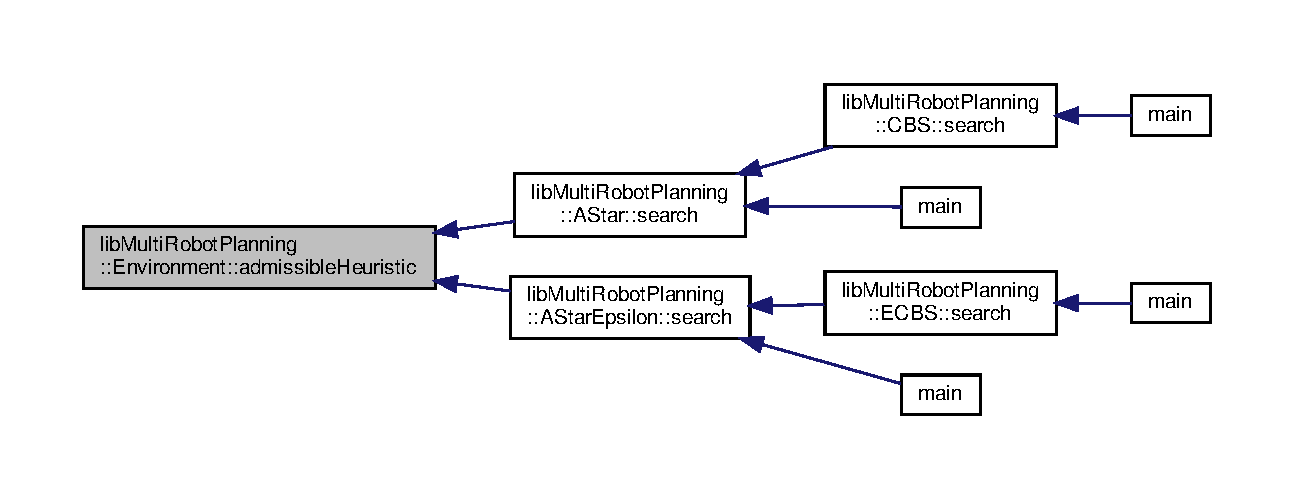
\includegraphics[width=350pt]{classlib_multi_robot_planning_1_1_environment_a125ea447e414ab365fea0eead52e47d7_icgraph}
\end{center}
\end{figure}
\mbox{\Hypertarget{classlib_multi_robot_planning_1_1_environment_a34aca235da8a5a1389ec71507c4191af}\label{classlib_multi_robot_planning_1_1_environment_a34aca235da8a5a1389ec71507c4191af}} 
\index{lib\+Multi\+Robot\+Planning\+::\+Environment@{lib\+Multi\+Robot\+Planning\+::\+Environment}!create\+Constraints\+From\+Conflict@{create\+Constraints\+From\+Conflict}}
\index{create\+Constraints\+From\+Conflict@{create\+Constraints\+From\+Conflict}!lib\+Multi\+Robot\+Planning\+::\+Environment@{lib\+Multi\+Robot\+Planning\+::\+Environment}}
\subsubsection{\texorpdfstring{create\+Constraints\+From\+Conflict()}{createConstraintsFromConflict()}}
{\footnotesize\ttfamily void lib\+Multi\+Robot\+Planning\+::\+Environment\+::create\+Constraints\+From\+Conflict (\begin{DoxyParamCaption}\item[{const \hyperlink{structlib_multi_robot_planning_1_1_conflict}{Conflict} \&}]{conflict,  }\item[{std\+::map$<$ size\+\_\+t, \hyperlink{structlib_multi_robot_planning_1_1_constraints}{Constraints} $>$ \&}]{constraints }\end{DoxyParamCaption})\hspace{0.3cm}{\ttfamily [inline]}}



Definition at line 562 of file environment.\+hpp.

Here is the caller graph for this function\+:
\nopagebreak
\begin{figure}[H]
\begin{center}
\leavevmode
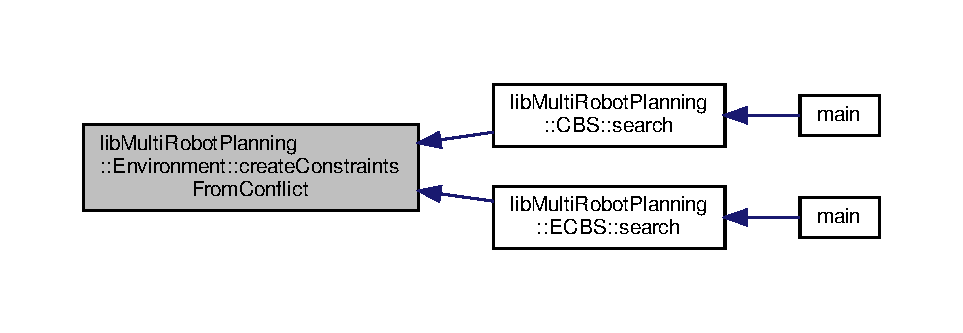
\includegraphics[width=350pt]{classlib_multi_robot_planning_1_1_environment_a34aca235da8a5a1389ec71507c4191af_icgraph}
\end{center}
\end{figure}
\mbox{\Hypertarget{classlib_multi_robot_planning_1_1_environment_a7854e1df446e52051492b724c0416956}\label{classlib_multi_robot_planning_1_1_environment_a7854e1df446e52051492b724c0416956}} 
\index{lib\+Multi\+Robot\+Planning\+::\+Environment@{lib\+Multi\+Robot\+Planning\+::\+Environment}!focal\+Heuristic@{focal\+Heuristic}}
\index{focal\+Heuristic@{focal\+Heuristic}!lib\+Multi\+Robot\+Planning\+::\+Environment@{lib\+Multi\+Robot\+Planning\+::\+Environment}}
\subsubsection{\texorpdfstring{focal\+Heuristic()}{focalHeuristic()}}
{\footnotesize\ttfamily int lib\+Multi\+Robot\+Planning\+::\+Environment\+::focal\+Heuristic (\begin{DoxyParamCaption}\item[{const std\+::vector$<$ \hyperlink{structlib_multi_robot_planning_1_1_plan_result}{Plan\+Result}$<$ \hyperlink{structlib_multi_robot_planning_1_1_state}{State}, \hyperlink{namespacelib_multi_robot_planning_aba73fb71693f86a324adfa0e41e1053d}{Action}, int $>$ $>$ \&}]{solution }\end{DoxyParamCaption})\hspace{0.3cm}{\ttfamily [inline]}}



Definition at line 356 of file environment.\+hpp.

Here is the call graph for this function\+:
\nopagebreak
\begin{figure}[H]
\begin{center}
\leavevmode
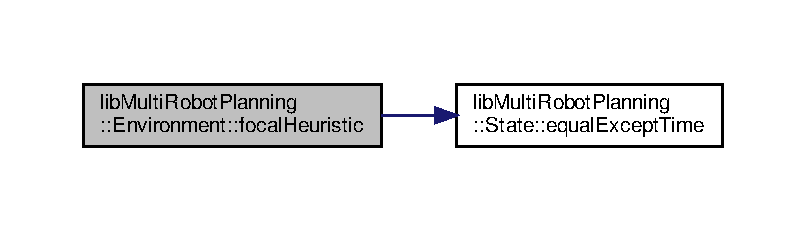
\includegraphics[width=350pt]{classlib_multi_robot_planning_1_1_environment_a7854e1df446e52051492b724c0416956_cgraph}
\end{center}
\end{figure}
Here is the caller graph for this function\+:
\nopagebreak
\begin{figure}[H]
\begin{center}
\leavevmode
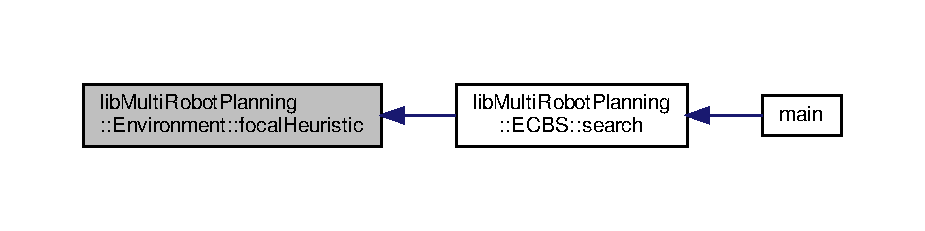
\includegraphics[width=350pt]{classlib_multi_robot_planning_1_1_environment_a7854e1df446e52051492b724c0416956_icgraph}
\end{center}
\end{figure}
\mbox{\Hypertarget{classlib_multi_robot_planning_1_1_environment_ac76b52b63f0bfbdde9dc6fed2520a0b6}\label{classlib_multi_robot_planning_1_1_environment_ac76b52b63f0bfbdde9dc6fed2520a0b6}} 
\index{lib\+Multi\+Robot\+Planning\+::\+Environment@{lib\+Multi\+Robot\+Planning\+::\+Environment}!focal\+State\+Heuristic@{focal\+State\+Heuristic}}
\index{focal\+State\+Heuristic@{focal\+State\+Heuristic}!lib\+Multi\+Robot\+Planning\+::\+Environment@{lib\+Multi\+Robot\+Planning\+::\+Environment}}
\subsubsection{\texorpdfstring{focal\+State\+Heuristic()}{focalStateHeuristic()}}
{\footnotesize\ttfamily int lib\+Multi\+Robot\+Planning\+::\+Environment\+::focal\+State\+Heuristic (\begin{DoxyParamCaption}\item[{const \hyperlink{structlib_multi_robot_planning_1_1_state}{State} \&}]{s,  }\item[{int}]{,  }\item[{const std\+::vector$<$ \hyperlink{structlib_multi_robot_planning_1_1_plan_result}{Plan\+Result}$<$ \hyperlink{structlib_multi_robot_planning_1_1_state}{State}, \hyperlink{namespacelib_multi_robot_planning_aba73fb71693f86a324adfa0e41e1053d}{Action}, int $>$ $>$ \&}]{solution }\end{DoxyParamCaption})\hspace{0.3cm}{\ttfamily [inline]}}



Definition at line 323 of file environment.\+hpp.

Here is the call graph for this function\+:
\nopagebreak
\begin{figure}[H]
\begin{center}
\leavevmode
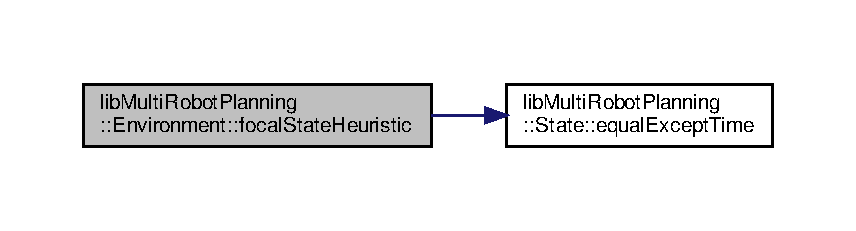
\includegraphics[width=350pt]{classlib_multi_robot_planning_1_1_environment_ac76b52b63f0bfbdde9dc6fed2520a0b6_cgraph}
\end{center}
\end{figure}
Here is the caller graph for this function\+:
\nopagebreak
\begin{figure}[H]
\begin{center}
\leavevmode
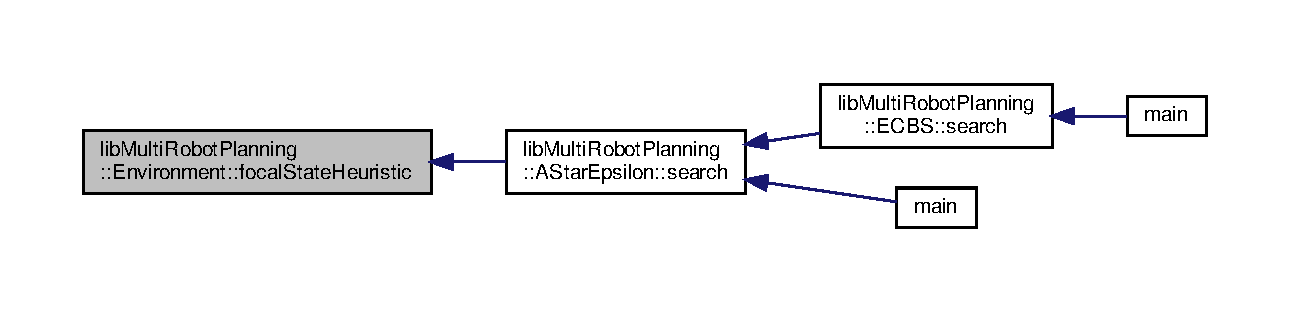
\includegraphics[width=350pt]{classlib_multi_robot_planning_1_1_environment_ac76b52b63f0bfbdde9dc6fed2520a0b6_icgraph}
\end{center}
\end{figure}
\mbox{\Hypertarget{classlib_multi_robot_planning_1_1_environment_adf9e6ca87f829fd0fdc185d85b29bb4e}\label{classlib_multi_robot_planning_1_1_environment_adf9e6ca87f829fd0fdc185d85b29bb4e}} 
\index{lib\+Multi\+Robot\+Planning\+::\+Environment@{lib\+Multi\+Robot\+Planning\+::\+Environment}!focal\+Transition\+Heuristic@{focal\+Transition\+Heuristic}}
\index{focal\+Transition\+Heuristic@{focal\+Transition\+Heuristic}!lib\+Multi\+Robot\+Planning\+::\+Environment@{lib\+Multi\+Robot\+Planning\+::\+Environment}}
\subsubsection{\texorpdfstring{focal\+Transition\+Heuristic()}{focalTransitionHeuristic()}}
{\footnotesize\ttfamily int lib\+Multi\+Robot\+Planning\+::\+Environment\+::focal\+Transition\+Heuristic (\begin{DoxyParamCaption}\item[{const \hyperlink{structlib_multi_robot_planning_1_1_state}{State} \&}]{s1a,  }\item[{const \hyperlink{structlib_multi_robot_planning_1_1_state}{State} \&}]{s1b,  }\item[{int}]{,  }\item[{int}]{,  }\item[{const std\+::vector$<$ \hyperlink{structlib_multi_robot_planning_1_1_plan_result}{Plan\+Result}$<$ \hyperlink{structlib_multi_robot_planning_1_1_state}{State}, \hyperlink{namespacelib_multi_robot_planning_aba73fb71693f86a324adfa0e41e1053d}{Action}, int $>$ $>$ \&}]{solution }\end{DoxyParamCaption})\hspace{0.3cm}{\ttfamily [inline]}}



Definition at line 339 of file environment.\+hpp.

Here is the call graph for this function\+:
\nopagebreak
\begin{figure}[H]
\begin{center}
\leavevmode
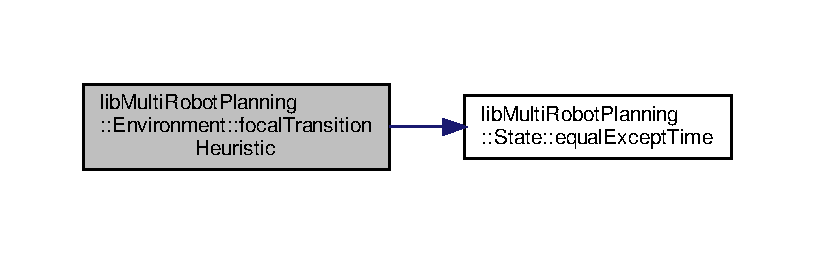
\includegraphics[width=350pt]{classlib_multi_robot_planning_1_1_environment_adf9e6ca87f829fd0fdc185d85b29bb4e_cgraph}
\end{center}
\end{figure}
Here is the caller graph for this function\+:
\nopagebreak
\begin{figure}[H]
\begin{center}
\leavevmode
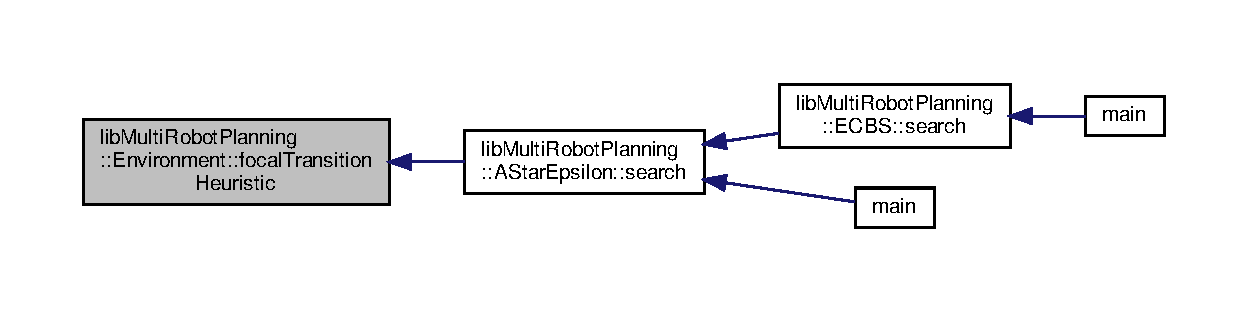
\includegraphics[width=350pt]{classlib_multi_robot_planning_1_1_environment_adf9e6ca87f829fd0fdc185d85b29bb4e_icgraph}
\end{center}
\end{figure}
\mbox{\Hypertarget{classlib_multi_robot_planning_1_1_environment_a1d47448bd35c1f46f70c6b7fa37e8146}\label{classlib_multi_robot_planning_1_1_environment_a1d47448bd35c1f46f70c6b7fa37e8146}} 
\index{lib\+Multi\+Robot\+Planning\+::\+Environment@{lib\+Multi\+Robot\+Planning\+::\+Environment}!get\+First\+Conflict@{get\+First\+Conflict}}
\index{get\+First\+Conflict@{get\+First\+Conflict}!lib\+Multi\+Robot\+Planning\+::\+Environment@{lib\+Multi\+Robot\+Planning\+::\+Environment}}
\subsubsection{\texorpdfstring{get\+First\+Conflict()}{getFirstConflict()}}
{\footnotesize\ttfamily bool lib\+Multi\+Robot\+Planning\+::\+Environment\+::get\+First\+Conflict (\begin{DoxyParamCaption}\item[{const std\+::vector$<$ \hyperlink{structlib_multi_robot_planning_1_1_plan_result}{Plan\+Result}$<$ \hyperlink{structlib_multi_robot_planning_1_1_state}{State}, \hyperlink{namespacelib_multi_robot_planning_aba73fb71693f86a324adfa0e41e1053d}{Action}, int $>$ $>$ \&}]{solution,  }\item[{\hyperlink{structlib_multi_robot_planning_1_1_conflict}{Conflict} \&}]{result }\end{DoxyParamCaption})\hspace{0.3cm}{\ttfamily [inline]}}



Definition at line 463 of file environment.\+hpp.

Here is the call graph for this function\+:
\nopagebreak
\begin{figure}[H]
\begin{center}
\leavevmode
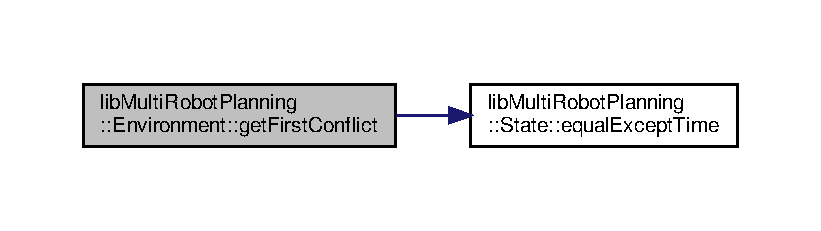
\includegraphics[width=350pt]{classlib_multi_robot_planning_1_1_environment_a1d47448bd35c1f46f70c6b7fa37e8146_cgraph}
\end{center}
\end{figure}
Here is the caller graph for this function\+:
\nopagebreak
\begin{figure}[H]
\begin{center}
\leavevmode
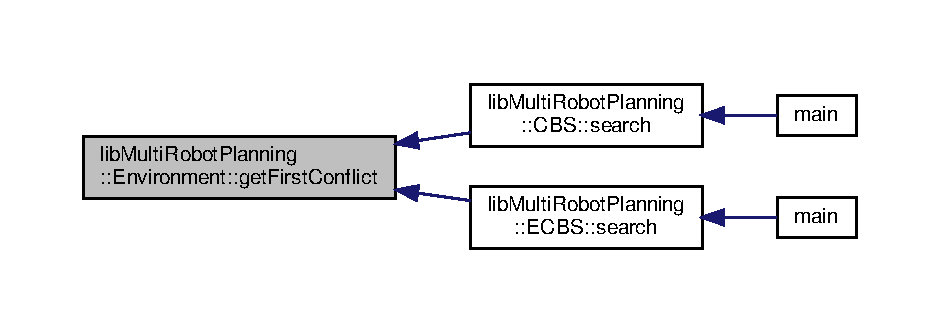
\includegraphics[width=350pt]{classlib_multi_robot_planning_1_1_environment_a1d47448bd35c1f46f70c6b7fa37e8146_icgraph}
\end{center}
\end{figure}
\mbox{\Hypertarget{classlib_multi_robot_planning_1_1_environment_ad0f11d7a4b91ea3d7f7fa39b9ffe9758}\label{classlib_multi_robot_planning_1_1_environment_ad0f11d7a4b91ea3d7f7fa39b9ffe9758}} 
\index{lib\+Multi\+Robot\+Planning\+::\+Environment@{lib\+Multi\+Robot\+Planning\+::\+Environment}!get\+Neighbors@{get\+Neighbors}}
\index{get\+Neighbors@{get\+Neighbors}!lib\+Multi\+Robot\+Planning\+::\+Environment@{lib\+Multi\+Robot\+Planning\+::\+Environment}}
\subsubsection{\texorpdfstring{get\+Neighbors()}{getNeighbors()}}
{\footnotesize\ttfamily void lib\+Multi\+Robot\+Planning\+::\+Environment\+::get\+Neighbors (\begin{DoxyParamCaption}\item[{const \hyperlink{structlib_multi_robot_planning_1_1_state}{State} \&}]{s,  }\item[{std\+::vector$<$ \hyperlink{structlib_multi_robot_planning_1_1_neighbor}{Neighbor}$<$ \hyperlink{structlib_multi_robot_planning_1_1_state}{State}, \hyperlink{namespacelib_multi_robot_planning_aba73fb71693f86a324adfa0e41e1053d}{Action}, int $>$ $>$ \&}]{neighbors }\end{DoxyParamCaption})\hspace{0.3cm}{\ttfamily [inline]}}



Definition at line 404 of file environment.\+hpp.

Here is the caller graph for this function\+:
\nopagebreak
\begin{figure}[H]
\begin{center}
\leavevmode
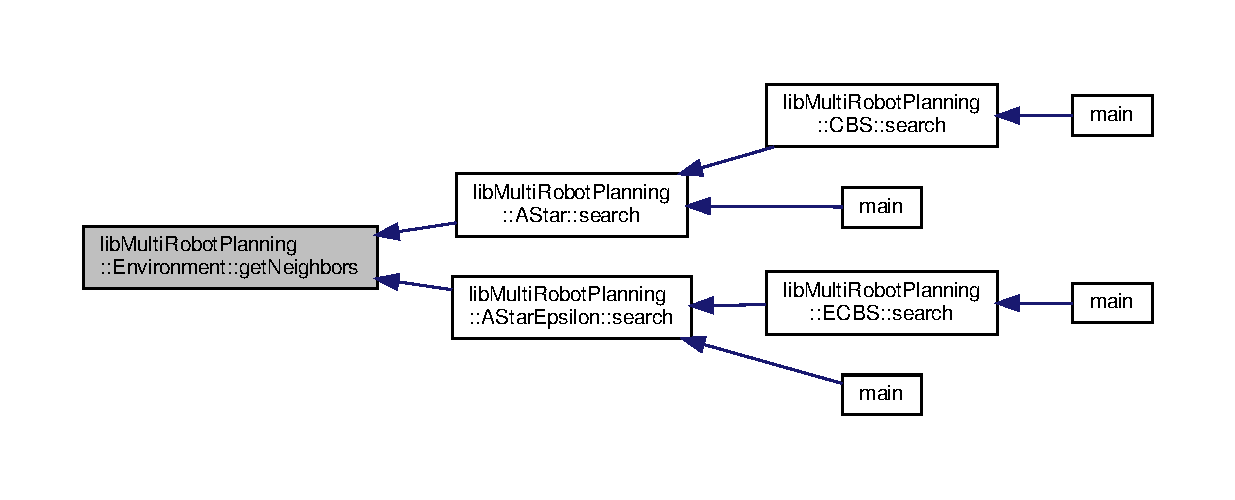
\includegraphics[width=350pt]{classlib_multi_robot_planning_1_1_environment_ad0f11d7a4b91ea3d7f7fa39b9ffe9758_icgraph}
\end{center}
\end{figure}
\mbox{\Hypertarget{classlib_multi_robot_planning_1_1_environment_ad3e27d5501dc54151814e015373e3ef7}\label{classlib_multi_robot_planning_1_1_environment_ad3e27d5501dc54151814e015373e3ef7}} 
\index{lib\+Multi\+Robot\+Planning\+::\+Environment@{lib\+Multi\+Robot\+Planning\+::\+Environment}!high\+Level\+Expanded@{high\+Level\+Expanded}}
\index{high\+Level\+Expanded@{high\+Level\+Expanded}!lib\+Multi\+Robot\+Planning\+::\+Environment@{lib\+Multi\+Robot\+Planning\+::\+Environment}}
\subsubsection{\texorpdfstring{high\+Level\+Expanded()}{highLevelExpanded()}}
{\footnotesize\ttfamily int lib\+Multi\+Robot\+Planning\+::\+Environment\+::high\+Level\+Expanded (\begin{DoxyParamCaption}{ }\end{DoxyParamCaption})\hspace{0.3cm}{\ttfamily [inline]}}



Definition at line 589 of file environment.\+hpp.

\mbox{\Hypertarget{classlib_multi_robot_planning_1_1_environment_a397c066a4202f0dccbb1346e2e3c8338}\label{classlib_multi_robot_planning_1_1_environment_a397c066a4202f0dccbb1346e2e3c8338}} 
\index{lib\+Multi\+Robot\+Planning\+::\+Environment@{lib\+Multi\+Robot\+Planning\+::\+Environment}!is\+Solution@{is\+Solution}}
\index{is\+Solution@{is\+Solution}!lib\+Multi\+Robot\+Planning\+::\+Environment@{lib\+Multi\+Robot\+Planning\+::\+Environment}}
\subsubsection{\texorpdfstring{is\+Solution()}{isSolution()}}
{\footnotesize\ttfamily bool lib\+Multi\+Robot\+Planning\+::\+Environment\+::is\+Solution (\begin{DoxyParamCaption}\item[{const \hyperlink{structlib_multi_robot_planning_1_1_state}{State} \&}]{s }\end{DoxyParamCaption})\hspace{0.3cm}{\ttfamily [inline]}}



Definition at line 399 of file environment.\+hpp.

Here is the caller graph for this function\+:
\nopagebreak
\begin{figure}[H]
\begin{center}
\leavevmode
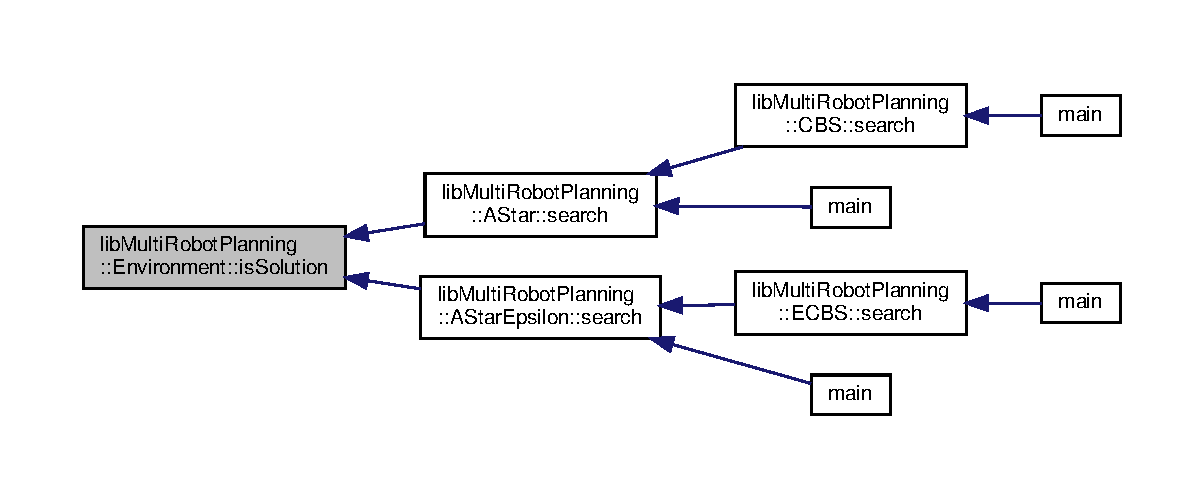
\includegraphics[width=350pt]{classlib_multi_robot_planning_1_1_environment_a397c066a4202f0dccbb1346e2e3c8338_icgraph}
\end{center}
\end{figure}
\mbox{\Hypertarget{classlib_multi_robot_planning_1_1_environment_a9dfe6761bd0b6d25628146cabfc08952}\label{classlib_multi_robot_planning_1_1_environment_a9dfe6761bd0b6d25628146cabfc08952}} 
\index{lib\+Multi\+Robot\+Planning\+::\+Environment@{lib\+Multi\+Robot\+Planning\+::\+Environment}!low\+Level\+Expanded@{low\+Level\+Expanded}}
\index{low\+Level\+Expanded@{low\+Level\+Expanded}!lib\+Multi\+Robot\+Planning\+::\+Environment@{lib\+Multi\+Robot\+Planning\+::\+Environment}}
\subsubsection{\texorpdfstring{low\+Level\+Expanded()}{lowLevelExpanded()}}
{\footnotesize\ttfamily int lib\+Multi\+Robot\+Planning\+::\+Environment\+::low\+Level\+Expanded (\begin{DoxyParamCaption}{ }\end{DoxyParamCaption}) const\hspace{0.3cm}{\ttfamily [inline]}}



Definition at line 591 of file environment.\+hpp.

\mbox{\Hypertarget{classlib_multi_robot_planning_1_1_environment_a5ce6ca98a37286cfe865b2b52b6c65aa}\label{classlib_multi_robot_planning_1_1_environment_a5ce6ca98a37286cfe865b2b52b6c65aa}} 
\index{lib\+Multi\+Robot\+Planning\+::\+Environment@{lib\+Multi\+Robot\+Planning\+::\+Environment}!on\+Expand\+High\+Level\+Node@{on\+Expand\+High\+Level\+Node}}
\index{on\+Expand\+High\+Level\+Node@{on\+Expand\+High\+Level\+Node}!lib\+Multi\+Robot\+Planning\+::\+Environment@{lib\+Multi\+Robot\+Planning\+::\+Environment}}
\subsubsection{\texorpdfstring{on\+Expand\+High\+Level\+Node()}{onExpandHighLevelNode()}}
{\footnotesize\ttfamily void lib\+Multi\+Robot\+Planning\+::\+Environment\+::on\+Expand\+High\+Level\+Node (\begin{DoxyParamCaption}\item[{int}]{ }\end{DoxyParamCaption})\hspace{0.3cm}{\ttfamily [inline]}}



Definition at line 582 of file environment.\+hpp.

Here is the caller graph for this function\+:
\nopagebreak
\begin{figure}[H]
\begin{center}
\leavevmode
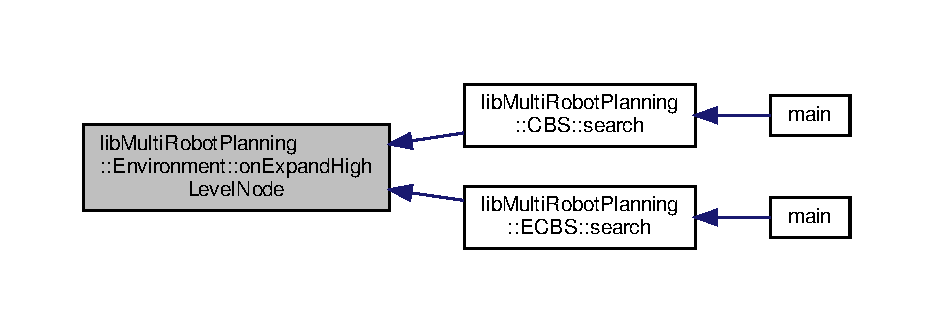
\includegraphics[width=350pt]{classlib_multi_robot_planning_1_1_environment_a5ce6ca98a37286cfe865b2b52b6c65aa_icgraph}
\end{center}
\end{figure}
\mbox{\Hypertarget{classlib_multi_robot_planning_1_1_environment_a022450370c58811b6407650e72a11230}\label{classlib_multi_robot_planning_1_1_environment_a022450370c58811b6407650e72a11230}} 
\index{lib\+Multi\+Robot\+Planning\+::\+Environment@{lib\+Multi\+Robot\+Planning\+::\+Environment}!on\+Expand\+Low\+Level\+Node@{on\+Expand\+Low\+Level\+Node}}
\index{on\+Expand\+Low\+Level\+Node@{on\+Expand\+Low\+Level\+Node}!lib\+Multi\+Robot\+Planning\+::\+Environment@{lib\+Multi\+Robot\+Planning\+::\+Environment}}
\subsubsection{\texorpdfstring{on\+Expand\+Low\+Level\+Node()}{onExpandLowLevelNode()}}
{\footnotesize\ttfamily void lib\+Multi\+Robot\+Planning\+::\+Environment\+::on\+Expand\+Low\+Level\+Node (\begin{DoxyParamCaption}\item[{const \hyperlink{structlib_multi_robot_planning_1_1_state}{State} \&}]{,  }\item[{int}]{,  }\item[{int}]{ }\end{DoxyParamCaption})\hspace{0.3cm}{\ttfamily [inline]}}



Definition at line 584 of file environment.\+hpp.

\mbox{\Hypertarget{classlib_multi_robot_planning_1_1_environment_afaf6184a779ac88068b4d405080d055c}\label{classlib_multi_robot_planning_1_1_environment_afaf6184a779ac88068b4d405080d055c}} 
\index{lib\+Multi\+Robot\+Planning\+::\+Environment@{lib\+Multi\+Robot\+Planning\+::\+Environment}!operator=@{operator=}}
\index{operator=@{operator=}!lib\+Multi\+Robot\+Planning\+::\+Environment@{lib\+Multi\+Robot\+Planning\+::\+Environment}}
\subsubsection{\texorpdfstring{operator=()}{operator=()}}
{\footnotesize\ttfamily \hyperlink{classlib_multi_robot_planning_1_1_environment}{Environment}\& lib\+Multi\+Robot\+Planning\+::\+Environment\+::operator= (\begin{DoxyParamCaption}\item[{const \hyperlink{classlib_multi_robot_planning_1_1_environment}{Environment} \&}]{ }\end{DoxyParamCaption})\hspace{0.3cm}{\ttfamily [delete]}}

\mbox{\Hypertarget{classlib_multi_robot_planning_1_1_environment_a7a664e26155157d558e0755204b74d11}\label{classlib_multi_robot_planning_1_1_environment_a7a664e26155157d558e0755204b74d11}} 
\index{lib\+Multi\+Robot\+Planning\+::\+Environment@{lib\+Multi\+Robot\+Planning\+::\+Environment}!set\+Low\+Level\+Context@{set\+Low\+Level\+Context}}
\index{set\+Low\+Level\+Context@{set\+Low\+Level\+Context}!lib\+Multi\+Robot\+Planning\+::\+Environment@{lib\+Multi\+Robot\+Planning\+::\+Environment}}
\subsubsection{\texorpdfstring{set\+Low\+Level\+Context()}{setLowLevelContext()}}
{\footnotesize\ttfamily void lib\+Multi\+Robot\+Planning\+::\+Environment\+::set\+Low\+Level\+Context (\begin{DoxyParamCaption}\item[{size\+\_\+t}]{agent\+Idx,  }\item[{const \hyperlink{structlib_multi_robot_planning_1_1_constraints}{Constraints} $\ast$}]{constraints }\end{DoxyParamCaption})\hspace{0.3cm}{\ttfamily [inline]}}



Definition at line 304 of file environment.\+hpp.



The documentation for this class was generated from the following file\+:\begin{DoxyCompactItemize}
\item 
third\+\_\+party/ecbs/include/\hyperlink{environment_8hpp}{environment.\+hpp}\end{DoxyCompactItemize}

\hypertarget{class_environment}{}\section{Environment Class Reference}
\label{class_environment}\index{Environment@{Environment}}
\subsection*{Public Member Functions}
\begin{DoxyCompactItemize}
\item 
\hyperlink{class_environment_a0ddc9c7b0862c1313b1ca99c2acb6d93}{Environment} (size\+\_\+t dimx, size\+\_\+t dimy, std\+::unordered\+\_\+set$<$ \hyperlink{struct_state}{State} $>$ obstacles, \hyperlink{struct_state}{State} goal)
\item 
int \hyperlink{class_environment_a171e702c373005a9d6e77b79daa365d9}{admissible\+Heuristic} (const \hyperlink{struct_state}{State} \&s)
\item 
bool \hyperlink{class_environment_aab14c04c6aaaf6b0d0f26f8b92d44400}{is\+Solution} (const \hyperlink{struct_state}{State} \&s)
\item 
void \hyperlink{class_environment_a4ae69480c6b9e716f282839dc4f323c0}{get\+Neighbors} (const \hyperlink{struct_state}{State} \&s, std\+::vector$<$ \hyperlink{structlib_multi_robot_planning_1_1_neighbor}{Neighbor}$<$ \hyperlink{struct_state}{State}, \hyperlink{a__star_8cpp_a8bb1ef53467e4f61410d12822d922498}{Action}, int $>$ $>$ \&neighbors)
\item 
void \hyperlink{class_environment_a37ccf718e3e1b4540dadbe89f1631ee6}{on\+Expand\+Node} (const \hyperlink{struct_state}{State} \&, int, int)
\item 
void \hyperlink{class_environment_a0c694f293bf62ef33dab4b878893bacf}{on\+Discover} (const \hyperlink{struct_state}{State} \&, int, int)
\item 
bool \hyperlink{class_environment_ad21a790ab0279b0f5b445e1f460dc971}{state\+Valid} (const \hyperlink{struct_state}{State} \&s)
\item 
\hyperlink{class_environment_aa5836d453e17e782e72d48437799e12d}{Environment} (size\+\_\+t dimx, size\+\_\+t dimy, size\+\_\+t dimz, std\+::unordered\+\_\+set$<$ \hyperlink{struct_state}{State} $>$ obstacles, \hyperlink{struct_state}{State} goal)
\item 
int \hyperlink{class_environment_a171e702c373005a9d6e77b79daa365d9}{admissible\+Heuristic} (const \hyperlink{struct_state}{State} \&s)
\item 
int \hyperlink{class_environment_a2ed02c2b1a21ae2aabb0e1758e945540}{focal\+State\+Heuristic} (const \hyperlink{struct_state}{State} \&, int g\+Score)
\item 
int \hyperlink{class_environment_ac799c113b3fd83ec89265786c9f29f37}{focal\+Transition\+Heuristic} (const \hyperlink{struct_state}{State} \&, const \hyperlink{struct_state}{State} \&, int g\+Score\+S1, int g\+Score\+S2)
\item 
bool \hyperlink{class_environment_aab14c04c6aaaf6b0d0f26f8b92d44400}{is\+Solution} (const \hyperlink{struct_state}{State} \&s)
\item 
void \hyperlink{class_environment_a4ae69480c6b9e716f282839dc4f323c0}{get\+Neighbors} (const \hyperlink{struct_state}{State} \&s, std\+::vector$<$ \hyperlink{structlib_multi_robot_planning_1_1_neighbor}{Neighbor}$<$ \hyperlink{struct_state}{State}, \hyperlink{a__star_8cpp_a8bb1ef53467e4f61410d12822d922498}{Action}, int $>$ $>$ \&neighbors)
\item 
void \hyperlink{class_environment_a37ccf718e3e1b4540dadbe89f1631ee6}{on\+Expand\+Node} (const \hyperlink{struct_state}{State} \&, int, int)
\item 
void \hyperlink{class_environment_a0c694f293bf62ef33dab4b878893bacf}{on\+Discover} (const \hyperlink{struct_state}{State} \&, int, int)
\item 
bool \hyperlink{class_environment_ad21a790ab0279b0f5b445e1f460dc971}{state\+Valid} (const \hyperlink{struct_state}{State} \&s)
\item 
\hyperlink{class_environment_a12b8baed8e6090b3eb528a27b1fecd0a}{Environment} (size\+\_\+t dimx, size\+\_\+t dimy, size\+\_\+t dimz, std\+::unordered\+\_\+set$<$ \hyperlink{struct_location}{Location} $>$ obstacles, std\+::vector$<$ \hyperlink{struct_location}{Location} $>$ goals)
\item 
\hyperlink{class_environment_abdb9fe9212fd5d47b5664df3e67c975f}{Environment} (const \hyperlink{class_environment}{Environment} \&)=delete
\item 
\hyperlink{class_environment}{Environment} \& \hyperlink{class_environment_a31a390fc46a51b9adab61b2511ef2a31}{operator=} (const \hyperlink{class_environment}{Environment} \&)=delete
\item 
void \hyperlink{class_environment_a56b6dff6d3af3fe6404936a14a259c56}{set\+Low\+Level\+Context} (size\+\_\+t agent\+Idx, const \hyperlink{struct_constraints}{Constraints} $\ast$constraints)
\item 
int \hyperlink{class_environment_a171e702c373005a9d6e77b79daa365d9}{admissible\+Heuristic} (const \hyperlink{struct_state}{State} \&s)
\item 
bool \hyperlink{class_environment_aab14c04c6aaaf6b0d0f26f8b92d44400}{is\+Solution} (const \hyperlink{struct_state}{State} \&s)
\item 
void \hyperlink{class_environment_a4ae69480c6b9e716f282839dc4f323c0}{get\+Neighbors} (const \hyperlink{struct_state}{State} \&s, std\+::vector$<$ \hyperlink{structlib_multi_robot_planning_1_1_neighbor}{Neighbor}$<$ \hyperlink{struct_state}{State}, \hyperlink{a__star_8cpp_a8bb1ef53467e4f61410d12822d922498}{Action}, int $>$ $>$ \&neighbors)
\item 
bool \hyperlink{class_environment_a666d55a1f0bbc038d3662b75f400faa4}{get\+First\+Conflict} (const std\+::vector$<$ \hyperlink{structlib_multi_robot_planning_1_1_plan_result}{Plan\+Result}$<$ \hyperlink{struct_state}{State}, \hyperlink{a__star_8cpp_a8bb1ef53467e4f61410d12822d922498}{Action}, int $>$ $>$ \&solution, \hyperlink{struct_conflict}{Conflict} \&result)
\item 
void \hyperlink{class_environment_a532b4870bfa50eb350e037dc8aa06291}{create\+Constraints\+From\+Conflict} (const \hyperlink{struct_conflict}{Conflict} \&conflict, std\+::map$<$ size\+\_\+t, \hyperlink{struct_constraints}{Constraints} $>$ \&constraints)
\item 
void \hyperlink{class_environment_ad8d27db649c723053fe9d90d97c0e4cd}{on\+Expand\+High\+Level\+Node} (int)
\item 
void \hyperlink{class_environment_ad00ee2a501b1e78f19c86a0d01e49d52}{on\+Expand\+Low\+Level\+Node} (const \hyperlink{struct_state}{State} \&, int, int)
\item 
int \hyperlink{class_environment_a117b88b2a1e0267cfe28d0a6545af72d}{high\+Level\+Expanded} ()
\item 
int \hyperlink{class_environment_af870f6d7c69f7401f5d724b0ee60308f}{low\+Level\+Expanded} () const
\item 
\hyperlink{class_environment_a12b8baed8e6090b3eb528a27b1fecd0a}{Environment} (size\+\_\+t dimx, size\+\_\+t dimy, size\+\_\+t dimz, std\+::unordered\+\_\+set$<$ \hyperlink{struct_location}{Location} $>$ obstacles, std\+::vector$<$ \hyperlink{struct_location}{Location} $>$ goals)
\item 
\hyperlink{class_environment_abdb9fe9212fd5d47b5664df3e67c975f}{Environment} (const \hyperlink{class_environment}{Environment} \&)=delete
\item 
\hyperlink{class_environment}{Environment} \& \hyperlink{class_environment_a31a390fc46a51b9adab61b2511ef2a31}{operator=} (const \hyperlink{class_environment}{Environment} \&)=delete
\item 
void \hyperlink{class_environment_a56b6dff6d3af3fe6404936a14a259c56}{set\+Low\+Level\+Context} (size\+\_\+t agent\+Idx, const \hyperlink{struct_constraints}{Constraints} $\ast$constraints)
\item 
int \hyperlink{class_environment_a171e702c373005a9d6e77b79daa365d9}{admissible\+Heuristic} (const \hyperlink{struct_state}{State} \&s)
\item 
int \hyperlink{class_environment_ae9c3ec27de36238b2d0ea75b8e2e80b1}{focal\+State\+Heuristic} (const \hyperlink{struct_state}{State} \&s, int, const std\+::vector$<$ \hyperlink{structlib_multi_robot_planning_1_1_plan_result}{Plan\+Result}$<$ \hyperlink{struct_state}{State}, \hyperlink{a__star_8cpp_a8bb1ef53467e4f61410d12822d922498}{Action}, int $>$ $>$ \&solution)
\item 
int \hyperlink{class_environment_a32ad1d8cf07f2104e033065fb95fadf6}{focal\+Transition\+Heuristic} (const \hyperlink{struct_state}{State} \&s1a, const \hyperlink{struct_state}{State} \&s1b, int, int, const std\+::vector$<$ \hyperlink{structlib_multi_robot_planning_1_1_plan_result}{Plan\+Result}$<$ \hyperlink{struct_state}{State}, \hyperlink{a__star_8cpp_a8bb1ef53467e4f61410d12822d922498}{Action}, int $>$ $>$ \&solution)
\item 
int \hyperlink{class_environment_a54d9038dd600b904b73936273d711fd0}{focal\+Heuristic} (const std\+::vector$<$ \hyperlink{structlib_multi_robot_planning_1_1_plan_result}{Plan\+Result}$<$ \hyperlink{struct_state}{State}, \hyperlink{a__star_8cpp_a8bb1ef53467e4f61410d12822d922498}{Action}, int $>$ $>$ \&solution)
\item 
bool \hyperlink{class_environment_aab14c04c6aaaf6b0d0f26f8b92d44400}{is\+Solution} (const \hyperlink{struct_state}{State} \&s)
\item 
void \hyperlink{class_environment_a4ae69480c6b9e716f282839dc4f323c0}{get\+Neighbors} (const \hyperlink{struct_state}{State} \&s, std\+::vector$<$ \hyperlink{structlib_multi_robot_planning_1_1_neighbor}{Neighbor}$<$ \hyperlink{struct_state}{State}, \hyperlink{a__star_8cpp_a8bb1ef53467e4f61410d12822d922498}{Action}, int $>$ $>$ \&neighbors)
\item 
bool \hyperlink{class_environment_a666d55a1f0bbc038d3662b75f400faa4}{get\+First\+Conflict} (const std\+::vector$<$ \hyperlink{structlib_multi_robot_planning_1_1_plan_result}{Plan\+Result}$<$ \hyperlink{struct_state}{State}, \hyperlink{a__star_8cpp_a8bb1ef53467e4f61410d12822d922498}{Action}, int $>$ $>$ \&solution, \hyperlink{struct_conflict}{Conflict} \&result)
\item 
void \hyperlink{class_environment_a532b4870bfa50eb350e037dc8aa06291}{create\+Constraints\+From\+Conflict} (const \hyperlink{struct_conflict}{Conflict} \&conflict, std\+::map$<$ size\+\_\+t, \hyperlink{struct_constraints}{Constraints} $>$ \&constraints)
\item 
void \hyperlink{class_environment_ad8d27db649c723053fe9d90d97c0e4cd}{on\+Expand\+High\+Level\+Node} (int)
\item 
void \hyperlink{class_environment_ad00ee2a501b1e78f19c86a0d01e49d52}{on\+Expand\+Low\+Level\+Node} (const \hyperlink{struct_state}{State} \&, int, int)
\item 
int \hyperlink{class_environment_a117b88b2a1e0267cfe28d0a6545af72d}{high\+Level\+Expanded} ()
\item 
int \hyperlink{class_environment_af870f6d7c69f7401f5d724b0ee60308f}{low\+Level\+Expanded} () const
\end{DoxyCompactItemize}


\subsection{Detailed Description}


Definition at line 70 of file a\+\_\+star.\+cpp.



\subsection{Constructor \& Destructor Documentation}
\mbox{\Hypertarget{class_environment_a0ddc9c7b0862c1313b1ca99c2acb6d93}\label{class_environment_a0ddc9c7b0862c1313b1ca99c2acb6d93}} 
\index{Environment@{Environment}!Environment@{Environment}}
\index{Environment@{Environment}!Environment@{Environment}}
\subsubsection{\texorpdfstring{Environment()}{Environment()}\hspace{0.1cm}{\footnotesize\ttfamily [1/6]}}
{\footnotesize\ttfamily Environment\+::\+Environment (\begin{DoxyParamCaption}\item[{size\+\_\+t}]{dimx,  }\item[{size\+\_\+t}]{dimy,  }\item[{std\+::unordered\+\_\+set$<$ \hyperlink{struct_state}{State} $>$}]{obstacles,  }\item[{\hyperlink{struct_state}{State}}]{goal }\end{DoxyParamCaption})\hspace{0.3cm}{\ttfamily [inline]}}



Definition at line 72 of file a\+\_\+star.\+cpp.

\mbox{\Hypertarget{class_environment_aa5836d453e17e782e72d48437799e12d}\label{class_environment_aa5836d453e17e782e72d48437799e12d}} 
\index{Environment@{Environment}!Environment@{Environment}}
\index{Environment@{Environment}!Environment@{Environment}}
\subsubsection{\texorpdfstring{Environment()}{Environment()}\hspace{0.1cm}{\footnotesize\ttfamily [2/6]}}
{\footnotesize\ttfamily Environment\+::\+Environment (\begin{DoxyParamCaption}\item[{size\+\_\+t}]{dimx,  }\item[{size\+\_\+t}]{dimy,  }\item[{size\+\_\+t}]{dimz,  }\item[{std\+::unordered\+\_\+set$<$ \hyperlink{struct_state}{State} $>$}]{obstacles,  }\item[{\hyperlink{struct_state}{State}}]{goal }\end{DoxyParamCaption})\hspace{0.3cm}{\ttfamily [inline]}}



Definition at line 82 of file a\+\_\+star\+\_\+epsilon.\+cpp.

\mbox{\Hypertarget{class_environment_a12b8baed8e6090b3eb528a27b1fecd0a}\label{class_environment_a12b8baed8e6090b3eb528a27b1fecd0a}} 
\index{Environment@{Environment}!Environment@{Environment}}
\index{Environment@{Environment}!Environment@{Environment}}
\subsubsection{\texorpdfstring{Environment()}{Environment()}\hspace{0.1cm}{\footnotesize\ttfamily [3/6]}}
{\footnotesize\ttfamily Environment\+::\+Environment (\begin{DoxyParamCaption}\item[{size\+\_\+t}]{dimx,  }\item[{size\+\_\+t}]{dimy,  }\item[{size\+\_\+t}]{dimz,  }\item[{std\+::unordered\+\_\+set$<$ \hyperlink{struct_location}{Location} $>$}]{obstacles,  }\item[{std\+::vector$<$ \hyperlink{struct_location}{Location} $>$}]{goals }\end{DoxyParamCaption})\hspace{0.3cm}{\ttfamily [inline]}}



Definition at line 269 of file cbs.\+cpp.

Here is the call graph for this function\+:
\nopagebreak
\begin{figure}[H]
\begin{center}
\leavevmode
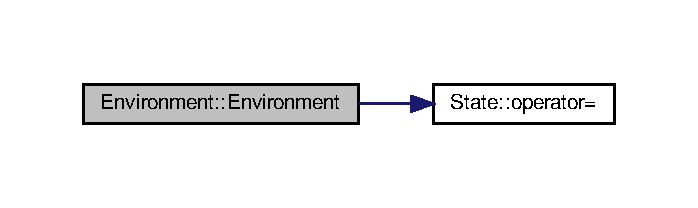
\includegraphics[width=335pt]{class_environment_a12b8baed8e6090b3eb528a27b1fecd0a_cgraph}
\end{center}
\end{figure}
\mbox{\Hypertarget{class_environment_abdb9fe9212fd5d47b5664df3e67c975f}\label{class_environment_abdb9fe9212fd5d47b5664df3e67c975f}} 
\index{Environment@{Environment}!Environment@{Environment}}
\index{Environment@{Environment}!Environment@{Environment}}
\subsubsection{\texorpdfstring{Environment()}{Environment()}\hspace{0.1cm}{\footnotesize\ttfamily [4/6]}}
{\footnotesize\ttfamily Environment\+::\+Environment (\begin{DoxyParamCaption}\item[{const \hyperlink{class_environment}{Environment} \&}]{ }\end{DoxyParamCaption})\hspace{0.3cm}{\ttfamily [delete]}}

\mbox{\Hypertarget{class_environment_a12b8baed8e6090b3eb528a27b1fecd0a}\label{class_environment_a12b8baed8e6090b3eb528a27b1fecd0a}} 
\index{Environment@{Environment}!Environment@{Environment}}
\index{Environment@{Environment}!Environment@{Environment}}
\subsubsection{\texorpdfstring{Environment()}{Environment()}\hspace{0.1cm}{\footnotesize\ttfamily [5/6]}}
{\footnotesize\ttfamily Environment\+::\+Environment (\begin{DoxyParamCaption}\item[{size\+\_\+t}]{dimx,  }\item[{size\+\_\+t}]{dimy,  }\item[{size\+\_\+t}]{dimz,  }\item[{std\+::unordered\+\_\+set$<$ \hyperlink{struct_location}{Location} $>$}]{obstacles,  }\item[{std\+::vector$<$ \hyperlink{struct_location}{Location} $>$}]{goals }\end{DoxyParamCaption})\hspace{0.3cm}{\ttfamily [inline]}}



Definition at line 269 of file ecbs.\+cpp.

Here is the call graph for this function\+:
\nopagebreak
\begin{figure}[H]
\begin{center}
\leavevmode
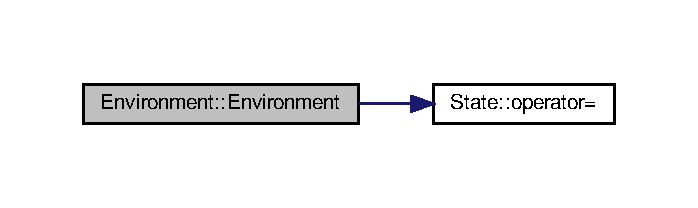
\includegraphics[width=335pt]{class_environment_a12b8baed8e6090b3eb528a27b1fecd0a_cgraph}
\end{center}
\end{figure}
\mbox{\Hypertarget{class_environment_abdb9fe9212fd5d47b5664df3e67c975f}\label{class_environment_abdb9fe9212fd5d47b5664df3e67c975f}} 
\index{Environment@{Environment}!Environment@{Environment}}
\index{Environment@{Environment}!Environment@{Environment}}
\subsubsection{\texorpdfstring{Environment()}{Environment()}\hspace{0.1cm}{\footnotesize\ttfamily [6/6]}}
{\footnotesize\ttfamily Environment\+::\+Environment (\begin{DoxyParamCaption}\item[{const \hyperlink{class_environment}{Environment} \&}]{ }\end{DoxyParamCaption})\hspace{0.3cm}{\ttfamily [delete]}}



\subsection{Member Function Documentation}
\mbox{\Hypertarget{class_environment_a171e702c373005a9d6e77b79daa365d9}\label{class_environment_a171e702c373005a9d6e77b79daa365d9}} 
\index{Environment@{Environment}!admissible\+Heuristic@{admissible\+Heuristic}}
\index{admissible\+Heuristic@{admissible\+Heuristic}!Environment@{Environment}}
\subsubsection{\texorpdfstring{admissible\+Heuristic()}{admissibleHeuristic()}\hspace{0.1cm}{\footnotesize\ttfamily [1/4]}}
{\footnotesize\ttfamily int Environment\+::admissible\+Heuristic (\begin{DoxyParamCaption}\item[{const \hyperlink{struct_state}{State} \&}]{s }\end{DoxyParamCaption})\hspace{0.3cm}{\ttfamily [inline]}}



Definition at line 80 of file a\+\_\+star.\+cpp.

\mbox{\Hypertarget{class_environment_a171e702c373005a9d6e77b79daa365d9}\label{class_environment_a171e702c373005a9d6e77b79daa365d9}} 
\index{Environment@{Environment}!admissible\+Heuristic@{admissible\+Heuristic}}
\index{admissible\+Heuristic@{admissible\+Heuristic}!Environment@{Environment}}
\subsubsection{\texorpdfstring{admissible\+Heuristic()}{admissibleHeuristic()}\hspace{0.1cm}{\footnotesize\ttfamily [2/4]}}
{\footnotesize\ttfamily int Environment\+::admissible\+Heuristic (\begin{DoxyParamCaption}\item[{const \hyperlink{struct_state}{State} \&}]{s }\end{DoxyParamCaption})\hspace{0.3cm}{\ttfamily [inline]}}



Definition at line 91 of file a\+\_\+star\+\_\+epsilon.\+cpp.

\mbox{\Hypertarget{class_environment_a171e702c373005a9d6e77b79daa365d9}\label{class_environment_a171e702c373005a9d6e77b79daa365d9}} 
\index{Environment@{Environment}!admissible\+Heuristic@{admissible\+Heuristic}}
\index{admissible\+Heuristic@{admissible\+Heuristic}!Environment@{Environment}}
\subsubsection{\texorpdfstring{admissible\+Heuristic()}{admissibleHeuristic()}\hspace{0.1cm}{\footnotesize\ttfamily [3/4]}}
{\footnotesize\ttfamily int Environment\+::admissible\+Heuristic (\begin{DoxyParamCaption}\item[{const \hyperlink{struct_state}{State} \&}]{s }\end{DoxyParamCaption})\hspace{0.3cm}{\ttfamily [inline]}}



Definition at line 299 of file cbs.\+cpp.

\mbox{\Hypertarget{class_environment_a171e702c373005a9d6e77b79daa365d9}\label{class_environment_a171e702c373005a9d6e77b79daa365d9}} 
\index{Environment@{Environment}!admissible\+Heuristic@{admissible\+Heuristic}}
\index{admissible\+Heuristic@{admissible\+Heuristic}!Environment@{Environment}}
\subsubsection{\texorpdfstring{admissible\+Heuristic()}{admissibleHeuristic()}\hspace{0.1cm}{\footnotesize\ttfamily [4/4]}}
{\footnotesize\ttfamily int Environment\+::admissible\+Heuristic (\begin{DoxyParamCaption}\item[{const \hyperlink{struct_state}{State} \&}]{s }\end{DoxyParamCaption})\hspace{0.3cm}{\ttfamily [inline]}}



Definition at line 299 of file ecbs.\+cpp.

\mbox{\Hypertarget{class_environment_a532b4870bfa50eb350e037dc8aa06291}\label{class_environment_a532b4870bfa50eb350e037dc8aa06291}} 
\index{Environment@{Environment}!create\+Constraints\+From\+Conflict@{create\+Constraints\+From\+Conflict}}
\index{create\+Constraints\+From\+Conflict@{create\+Constraints\+From\+Conflict}!Environment@{Environment}}
\subsubsection{\texorpdfstring{create\+Constraints\+From\+Conflict()}{createConstraintsFromConflict()}\hspace{0.1cm}{\footnotesize\ttfamily [1/2]}}
{\footnotesize\ttfamily void Environment\+::create\+Constraints\+From\+Conflict (\begin{DoxyParamCaption}\item[{const \hyperlink{struct_conflict}{Conflict} \&}]{conflict,  }\item[{std\+::map$<$ size\+\_\+t, \hyperlink{struct_constraints}{Constraints} $>$ \&}]{constraints }\end{DoxyParamCaption})\hspace{0.3cm}{\ttfamily [inline]}}



Definition at line 427 of file cbs.\+cpp.

\mbox{\Hypertarget{class_environment_a532b4870bfa50eb350e037dc8aa06291}\label{class_environment_a532b4870bfa50eb350e037dc8aa06291}} 
\index{Environment@{Environment}!create\+Constraints\+From\+Conflict@{create\+Constraints\+From\+Conflict}}
\index{create\+Constraints\+From\+Conflict@{create\+Constraints\+From\+Conflict}!Environment@{Environment}}
\subsubsection{\texorpdfstring{create\+Constraints\+From\+Conflict()}{createConstraintsFromConflict()}\hspace{0.1cm}{\footnotesize\ttfamily [2/2]}}
{\footnotesize\ttfamily void Environment\+::create\+Constraints\+From\+Conflict (\begin{DoxyParamCaption}\item[{const \hyperlink{struct_conflict}{Conflict} \&}]{conflict,  }\item[{std\+::map$<$ size\+\_\+t, \hyperlink{struct_constraints}{Constraints} $>$ \&}]{constraints }\end{DoxyParamCaption})\hspace{0.3cm}{\ttfamily [inline]}}



Definition at line 496 of file ecbs.\+cpp.

\mbox{\Hypertarget{class_environment_a54d9038dd600b904b73936273d711fd0}\label{class_environment_a54d9038dd600b904b73936273d711fd0}} 
\index{Environment@{Environment}!focal\+Heuristic@{focal\+Heuristic}}
\index{focal\+Heuristic@{focal\+Heuristic}!Environment@{Environment}}
\subsubsection{\texorpdfstring{focal\+Heuristic()}{focalHeuristic()}}
{\footnotesize\ttfamily int Environment\+::focal\+Heuristic (\begin{DoxyParamCaption}\item[{const std\+::vector$<$ \hyperlink{structlib_multi_robot_planning_1_1_plan_result}{Plan\+Result}$<$ \hyperlink{struct_state}{State}, \hyperlink{a__star_8cpp_a8bb1ef53467e4f61410d12822d922498}{Action}, int $>$ $>$ \&}]{solution }\end{DoxyParamCaption})\hspace{0.3cm}{\ttfamily [inline]}}



Definition at line 339 of file ecbs.\+cpp.

Here is the call graph for this function\+:
\nopagebreak
\begin{figure}[H]
\begin{center}
\leavevmode
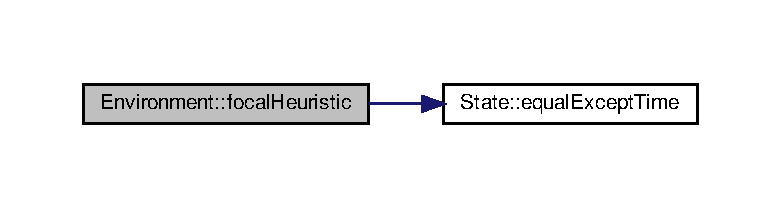
\includegraphics[width=350pt]{class_environment_a54d9038dd600b904b73936273d711fd0_cgraph}
\end{center}
\end{figure}
\mbox{\Hypertarget{class_environment_a2ed02c2b1a21ae2aabb0e1758e945540}\label{class_environment_a2ed02c2b1a21ae2aabb0e1758e945540}} 
\index{Environment@{Environment}!focal\+State\+Heuristic@{focal\+State\+Heuristic}}
\index{focal\+State\+Heuristic@{focal\+State\+Heuristic}!Environment@{Environment}}
\subsubsection{\texorpdfstring{focal\+State\+Heuristic()}{focalStateHeuristic()}\hspace{0.1cm}{\footnotesize\ttfamily [1/2]}}
{\footnotesize\ttfamily int Environment\+::focal\+State\+Heuristic (\begin{DoxyParamCaption}\item[{const \hyperlink{struct_state}{State} \&}]{,  }\item[{int}]{g\+Score }\end{DoxyParamCaption})\hspace{0.3cm}{\ttfamily [inline]}}



Definition at line 96 of file a\+\_\+star\+\_\+epsilon.\+cpp.

\mbox{\Hypertarget{class_environment_ae9c3ec27de36238b2d0ea75b8e2e80b1}\label{class_environment_ae9c3ec27de36238b2d0ea75b8e2e80b1}} 
\index{Environment@{Environment}!focal\+State\+Heuristic@{focal\+State\+Heuristic}}
\index{focal\+State\+Heuristic@{focal\+State\+Heuristic}!Environment@{Environment}}
\subsubsection{\texorpdfstring{focal\+State\+Heuristic()}{focalStateHeuristic()}\hspace{0.1cm}{\footnotesize\ttfamily [2/2]}}
{\footnotesize\ttfamily int Environment\+::focal\+State\+Heuristic (\begin{DoxyParamCaption}\item[{const \hyperlink{struct_state}{State} \&}]{s,  }\item[{int}]{,  }\item[{const std\+::vector$<$ \hyperlink{structlib_multi_robot_planning_1_1_plan_result}{Plan\+Result}$<$ \hyperlink{struct_state}{State}, \hyperlink{a__star_8cpp_a8bb1ef53467e4f61410d12822d922498}{Action}, int $>$ $>$ \&}]{solution }\end{DoxyParamCaption})\hspace{0.3cm}{\ttfamily [inline]}}



Definition at line 306 of file ecbs.\+cpp.

Here is the call graph for this function\+:
\nopagebreak
\begin{figure}[H]
\begin{center}
\leavevmode
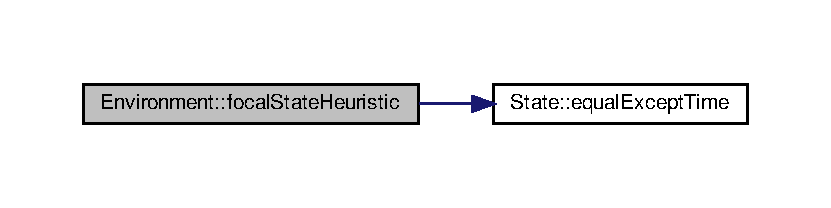
\includegraphics[width=350pt]{class_environment_ae9c3ec27de36238b2d0ea75b8e2e80b1_cgraph}
\end{center}
\end{figure}
\mbox{\Hypertarget{class_environment_ac799c113b3fd83ec89265786c9f29f37}\label{class_environment_ac799c113b3fd83ec89265786c9f29f37}} 
\index{Environment@{Environment}!focal\+Transition\+Heuristic@{focal\+Transition\+Heuristic}}
\index{focal\+Transition\+Heuristic@{focal\+Transition\+Heuristic}!Environment@{Environment}}
\subsubsection{\texorpdfstring{focal\+Transition\+Heuristic()}{focalTransitionHeuristic()}\hspace{0.1cm}{\footnotesize\ttfamily [1/2]}}
{\footnotesize\ttfamily int Environment\+::focal\+Transition\+Heuristic (\begin{DoxyParamCaption}\item[{const \hyperlink{struct_state}{State} \&}]{,  }\item[{const \hyperlink{struct_state}{State} \&}]{,  }\item[{int}]{g\+Score\+S1,  }\item[{int}]{g\+Score\+S2 }\end{DoxyParamCaption})\hspace{0.3cm}{\ttfamily [inline]}}



Definition at line 101 of file a\+\_\+star\+\_\+epsilon.\+cpp.

\mbox{\Hypertarget{class_environment_a32ad1d8cf07f2104e033065fb95fadf6}\label{class_environment_a32ad1d8cf07f2104e033065fb95fadf6}} 
\index{Environment@{Environment}!focal\+Transition\+Heuristic@{focal\+Transition\+Heuristic}}
\index{focal\+Transition\+Heuristic@{focal\+Transition\+Heuristic}!Environment@{Environment}}
\subsubsection{\texorpdfstring{focal\+Transition\+Heuristic()}{focalTransitionHeuristic()}\hspace{0.1cm}{\footnotesize\ttfamily [2/2]}}
{\footnotesize\ttfamily int Environment\+::focal\+Transition\+Heuristic (\begin{DoxyParamCaption}\item[{const \hyperlink{struct_state}{State} \&}]{s1a,  }\item[{const \hyperlink{struct_state}{State} \&}]{s1b,  }\item[{int}]{,  }\item[{int}]{,  }\item[{const std\+::vector$<$ \hyperlink{structlib_multi_robot_planning_1_1_plan_result}{Plan\+Result}$<$ \hyperlink{struct_state}{State}, \hyperlink{a__star_8cpp_a8bb1ef53467e4f61410d12822d922498}{Action}, int $>$ $>$ \&}]{solution }\end{DoxyParamCaption})\hspace{0.3cm}{\ttfamily [inline]}}



Definition at line 322 of file ecbs.\+cpp.

Here is the call graph for this function\+:
\nopagebreak
\begin{figure}[H]
\begin{center}
\leavevmode
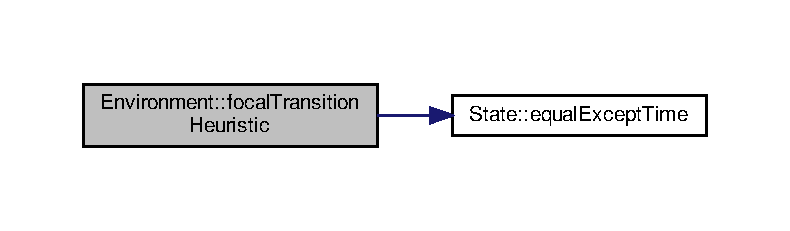
\includegraphics[width=350pt]{class_environment_a32ad1d8cf07f2104e033065fb95fadf6_cgraph}
\end{center}
\end{figure}
\mbox{\Hypertarget{class_environment_a666d55a1f0bbc038d3662b75f400faa4}\label{class_environment_a666d55a1f0bbc038d3662b75f400faa4}} 
\index{Environment@{Environment}!get\+First\+Conflict@{get\+First\+Conflict}}
\index{get\+First\+Conflict@{get\+First\+Conflict}!Environment@{Environment}}
\subsubsection{\texorpdfstring{get\+First\+Conflict()}{getFirstConflict()}\hspace{0.1cm}{\footnotesize\ttfamily [1/2]}}
{\footnotesize\ttfamily bool Environment\+::get\+First\+Conflict (\begin{DoxyParamCaption}\item[{const std\+::vector$<$ \hyperlink{structlib_multi_robot_planning_1_1_plan_result}{Plan\+Result}$<$ \hyperlink{struct_state}{State}, \hyperlink{a__star_8cpp_a8bb1ef53467e4f61410d12822d922498}{Action}, int $>$ $>$ \&}]{solution,  }\item[{\hyperlink{struct_conflict}{Conflict} \&}]{result }\end{DoxyParamCaption})\hspace{0.3cm}{\ttfamily [inline]}}



Definition at line 371 of file cbs.\+cpp.

Here is the call graph for this function\+:
\nopagebreak
\begin{figure}[H]
\begin{center}
\leavevmode
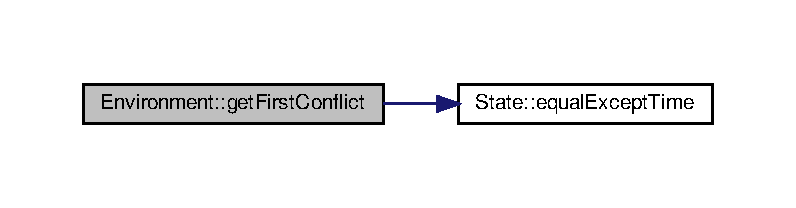
\includegraphics[width=350pt]{class_environment_a666d55a1f0bbc038d3662b75f400faa4_cgraph}
\end{center}
\end{figure}
\mbox{\Hypertarget{class_environment_a666d55a1f0bbc038d3662b75f400faa4}\label{class_environment_a666d55a1f0bbc038d3662b75f400faa4}} 
\index{Environment@{Environment}!get\+First\+Conflict@{get\+First\+Conflict}}
\index{get\+First\+Conflict@{get\+First\+Conflict}!Environment@{Environment}}
\subsubsection{\texorpdfstring{get\+First\+Conflict()}{getFirstConflict()}\hspace{0.1cm}{\footnotesize\ttfamily [2/2]}}
{\footnotesize\ttfamily bool Environment\+::get\+First\+Conflict (\begin{DoxyParamCaption}\item[{const std\+::vector$<$ \hyperlink{structlib_multi_robot_planning_1_1_plan_result}{Plan\+Result}$<$ \hyperlink{struct_state}{State}, \hyperlink{a__star_8cpp_a8bb1ef53467e4f61410d12822d922498}{Action}, int $>$ $>$ \&}]{solution,  }\item[{\hyperlink{struct_conflict}{Conflict} \&}]{result }\end{DoxyParamCaption})\hspace{0.3cm}{\ttfamily [inline]}}



Definition at line 440 of file ecbs.\+cpp.

Here is the call graph for this function\+:
\nopagebreak
\begin{figure}[H]
\begin{center}
\leavevmode
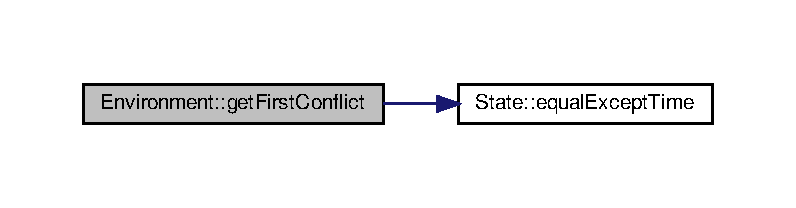
\includegraphics[width=350pt]{class_environment_a666d55a1f0bbc038d3662b75f400faa4_cgraph}
\end{center}
\end{figure}
\mbox{\Hypertarget{class_environment_a4ae69480c6b9e716f282839dc4f323c0}\label{class_environment_a4ae69480c6b9e716f282839dc4f323c0}} 
\index{Environment@{Environment}!get\+Neighbors@{get\+Neighbors}}
\index{get\+Neighbors@{get\+Neighbors}!Environment@{Environment}}
\subsubsection{\texorpdfstring{get\+Neighbors()}{getNeighbors()}\hspace{0.1cm}{\footnotesize\ttfamily [1/4]}}
{\footnotesize\ttfamily void Environment\+::get\+Neighbors (\begin{DoxyParamCaption}\item[{const \hyperlink{struct_state}{State} \&}]{s,  }\item[{std\+::vector$<$ \hyperlink{structlib_multi_robot_planning_1_1_neighbor}{Neighbor}$<$ \hyperlink{struct_state}{State}, \hyperlink{a__star_8cpp_a8bb1ef53467e4f61410d12822d922498}{Action}, int $>$ $>$ \&}]{neighbors }\end{DoxyParamCaption})\hspace{0.3cm}{\ttfamily [inline]}}



Definition at line 86 of file a\+\_\+star.\+cpp.

\mbox{\Hypertarget{class_environment_a4ae69480c6b9e716f282839dc4f323c0}\label{class_environment_a4ae69480c6b9e716f282839dc4f323c0}} 
\index{Environment@{Environment}!get\+Neighbors@{get\+Neighbors}}
\index{get\+Neighbors@{get\+Neighbors}!Environment@{Environment}}
\subsubsection{\texorpdfstring{get\+Neighbors()}{getNeighbors()}\hspace{0.1cm}{\footnotesize\ttfamily [2/4]}}
{\footnotesize\ttfamily void Environment\+::get\+Neighbors (\begin{DoxyParamCaption}\item[{const \hyperlink{struct_state}{State} \&}]{s,  }\item[{std\+::vector$<$ \hyperlink{structlib_multi_robot_planning_1_1_neighbor}{Neighbor}$<$ \hyperlink{struct_state}{State}, \hyperlink{a__star_8cpp_a8bb1ef53467e4f61410d12822d922498}{Action}, int $>$ $>$ \&}]{neighbors }\end{DoxyParamCaption})\hspace{0.3cm}{\ttfamily [inline]}}



Definition at line 109 of file a\+\_\+star\+\_\+epsilon.\+cpp.

\mbox{\Hypertarget{class_environment_a4ae69480c6b9e716f282839dc4f323c0}\label{class_environment_a4ae69480c6b9e716f282839dc4f323c0}} 
\index{Environment@{Environment}!get\+Neighbors@{get\+Neighbors}}
\index{get\+Neighbors@{get\+Neighbors}!Environment@{Environment}}
\subsubsection{\texorpdfstring{get\+Neighbors()}{getNeighbors()}\hspace{0.1cm}{\footnotesize\ttfamily [3/4]}}
{\footnotesize\ttfamily void Environment\+::get\+Neighbors (\begin{DoxyParamCaption}\item[{const \hyperlink{struct_state}{State} \&}]{s,  }\item[{std\+::vector$<$ \hyperlink{structlib_multi_robot_planning_1_1_neighbor}{Neighbor}$<$ \hyperlink{struct_state}{State}, \hyperlink{a__star_8cpp_a8bb1ef53467e4f61410d12822d922498}{Action}, int $>$ $>$ \&}]{neighbors }\end{DoxyParamCaption})\hspace{0.3cm}{\ttfamily [inline]}}



Definition at line 313 of file cbs.\+cpp.

\mbox{\Hypertarget{class_environment_a4ae69480c6b9e716f282839dc4f323c0}\label{class_environment_a4ae69480c6b9e716f282839dc4f323c0}} 
\index{Environment@{Environment}!get\+Neighbors@{get\+Neighbors}}
\index{get\+Neighbors@{get\+Neighbors}!Environment@{Environment}}
\subsubsection{\texorpdfstring{get\+Neighbors()}{getNeighbors()}\hspace{0.1cm}{\footnotesize\ttfamily [4/4]}}
{\footnotesize\ttfamily void Environment\+::get\+Neighbors (\begin{DoxyParamCaption}\item[{const \hyperlink{struct_state}{State} \&}]{s,  }\item[{std\+::vector$<$ \hyperlink{structlib_multi_robot_planning_1_1_neighbor}{Neighbor}$<$ \hyperlink{struct_state}{State}, \hyperlink{a__star_8cpp_a8bb1ef53467e4f61410d12822d922498}{Action}, int $>$ $>$ \&}]{neighbors }\end{DoxyParamCaption})\hspace{0.3cm}{\ttfamily [inline]}}



Definition at line 381 of file ecbs.\+cpp.

\mbox{\Hypertarget{class_environment_a117b88b2a1e0267cfe28d0a6545af72d}\label{class_environment_a117b88b2a1e0267cfe28d0a6545af72d}} 
\index{Environment@{Environment}!high\+Level\+Expanded@{high\+Level\+Expanded}}
\index{high\+Level\+Expanded@{high\+Level\+Expanded}!Environment@{Environment}}
\subsubsection{\texorpdfstring{high\+Level\+Expanded()}{highLevelExpanded()}\hspace{0.1cm}{\footnotesize\ttfamily [1/2]}}
{\footnotesize\ttfamily int Environment\+::high\+Level\+Expanded (\begin{DoxyParamCaption}{ }\end{DoxyParamCaption})\hspace{0.3cm}{\ttfamily [inline]}}



Definition at line 454 of file cbs.\+cpp.

Here is the caller graph for this function\+:
\nopagebreak
\begin{figure}[H]
\begin{center}
\leavevmode
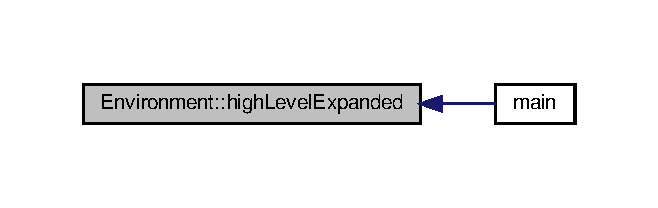
\includegraphics[width=316pt]{class_environment_a117b88b2a1e0267cfe28d0a6545af72d_icgraph}
\end{center}
\end{figure}
\mbox{\Hypertarget{class_environment_a117b88b2a1e0267cfe28d0a6545af72d}\label{class_environment_a117b88b2a1e0267cfe28d0a6545af72d}} 
\index{Environment@{Environment}!high\+Level\+Expanded@{high\+Level\+Expanded}}
\index{high\+Level\+Expanded@{high\+Level\+Expanded}!Environment@{Environment}}
\subsubsection{\texorpdfstring{high\+Level\+Expanded()}{highLevelExpanded()}\hspace{0.1cm}{\footnotesize\ttfamily [2/2]}}
{\footnotesize\ttfamily int Environment\+::high\+Level\+Expanded (\begin{DoxyParamCaption}{ }\end{DoxyParamCaption})\hspace{0.3cm}{\ttfamily [inline]}}



Definition at line 523 of file ecbs.\+cpp.

\mbox{\Hypertarget{class_environment_aab14c04c6aaaf6b0d0f26f8b92d44400}\label{class_environment_aab14c04c6aaaf6b0d0f26f8b92d44400}} 
\index{Environment@{Environment}!is\+Solution@{is\+Solution}}
\index{is\+Solution@{is\+Solution}!Environment@{Environment}}
\subsubsection{\texorpdfstring{is\+Solution()}{isSolution()}\hspace{0.1cm}{\footnotesize\ttfamily [1/4]}}
{\footnotesize\ttfamily bool Environment\+::is\+Solution (\begin{DoxyParamCaption}\item[{const \hyperlink{struct_state}{State} \&}]{s }\end{DoxyParamCaption})\hspace{0.3cm}{\ttfamily [inline]}}



Definition at line 84 of file a\+\_\+star.\+cpp.

\mbox{\Hypertarget{class_environment_aab14c04c6aaaf6b0d0f26f8b92d44400}\label{class_environment_aab14c04c6aaaf6b0d0f26f8b92d44400}} 
\index{Environment@{Environment}!is\+Solution@{is\+Solution}}
\index{is\+Solution@{is\+Solution}!Environment@{Environment}}
\subsubsection{\texorpdfstring{is\+Solution()}{isSolution()}\hspace{0.1cm}{\footnotesize\ttfamily [2/4]}}
{\footnotesize\ttfamily bool Environment\+::is\+Solution (\begin{DoxyParamCaption}\item[{const \hyperlink{struct_state}{State} \&}]{s }\end{DoxyParamCaption})\hspace{0.3cm}{\ttfamily [inline]}}



Definition at line 107 of file a\+\_\+star\+\_\+epsilon.\+cpp.

\mbox{\Hypertarget{class_environment_aab14c04c6aaaf6b0d0f26f8b92d44400}\label{class_environment_aab14c04c6aaaf6b0d0f26f8b92d44400}} 
\index{Environment@{Environment}!is\+Solution@{is\+Solution}}
\index{is\+Solution@{is\+Solution}!Environment@{Environment}}
\subsubsection{\texorpdfstring{is\+Solution()}{isSolution()}\hspace{0.1cm}{\footnotesize\ttfamily [3/4]}}
{\footnotesize\ttfamily bool Environment\+::is\+Solution (\begin{DoxyParamCaption}\item[{const \hyperlink{struct_state}{State} \&}]{s }\end{DoxyParamCaption})\hspace{0.3cm}{\ttfamily [inline]}}



Definition at line 308 of file cbs.\+cpp.

\mbox{\Hypertarget{class_environment_aab14c04c6aaaf6b0d0f26f8b92d44400}\label{class_environment_aab14c04c6aaaf6b0d0f26f8b92d44400}} 
\index{Environment@{Environment}!is\+Solution@{is\+Solution}}
\index{is\+Solution@{is\+Solution}!Environment@{Environment}}
\subsubsection{\texorpdfstring{is\+Solution()}{isSolution()}\hspace{0.1cm}{\footnotesize\ttfamily [4/4]}}
{\footnotesize\ttfamily bool Environment\+::is\+Solution (\begin{DoxyParamCaption}\item[{const \hyperlink{struct_state}{State} \&}]{s }\end{DoxyParamCaption})\hspace{0.3cm}{\ttfamily [inline]}}



Definition at line 376 of file ecbs.\+cpp.

\mbox{\Hypertarget{class_environment_af870f6d7c69f7401f5d724b0ee60308f}\label{class_environment_af870f6d7c69f7401f5d724b0ee60308f}} 
\index{Environment@{Environment}!low\+Level\+Expanded@{low\+Level\+Expanded}}
\index{low\+Level\+Expanded@{low\+Level\+Expanded}!Environment@{Environment}}
\subsubsection{\texorpdfstring{low\+Level\+Expanded()}{lowLevelExpanded()}\hspace{0.1cm}{\footnotesize\ttfamily [1/2]}}
{\footnotesize\ttfamily int Environment\+::low\+Level\+Expanded (\begin{DoxyParamCaption}{ }\end{DoxyParamCaption}) const\hspace{0.3cm}{\ttfamily [inline]}}



Definition at line 456 of file cbs.\+cpp.

Here is the caller graph for this function\+:
\nopagebreak
\begin{figure}[H]
\begin{center}
\leavevmode
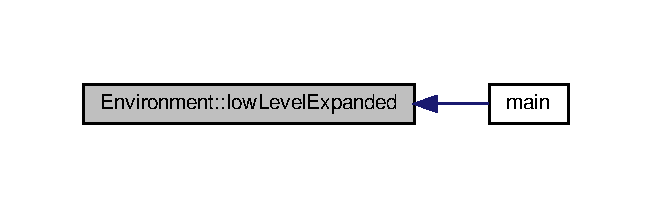
\includegraphics[width=313pt]{class_environment_af870f6d7c69f7401f5d724b0ee60308f_icgraph}
\end{center}
\end{figure}
\mbox{\Hypertarget{class_environment_af870f6d7c69f7401f5d724b0ee60308f}\label{class_environment_af870f6d7c69f7401f5d724b0ee60308f}} 
\index{Environment@{Environment}!low\+Level\+Expanded@{low\+Level\+Expanded}}
\index{low\+Level\+Expanded@{low\+Level\+Expanded}!Environment@{Environment}}
\subsubsection{\texorpdfstring{low\+Level\+Expanded()}{lowLevelExpanded()}\hspace{0.1cm}{\footnotesize\ttfamily [2/2]}}
{\footnotesize\ttfamily int Environment\+::low\+Level\+Expanded (\begin{DoxyParamCaption}{ }\end{DoxyParamCaption}) const\hspace{0.3cm}{\ttfamily [inline]}}



Definition at line 525 of file ecbs.\+cpp.

\mbox{\Hypertarget{class_environment_a0c694f293bf62ef33dab4b878893bacf}\label{class_environment_a0c694f293bf62ef33dab4b878893bacf}} 
\index{Environment@{Environment}!on\+Discover@{on\+Discover}}
\index{on\+Discover@{on\+Discover}!Environment@{Environment}}
\subsubsection{\texorpdfstring{on\+Discover()}{onDiscover()}\hspace{0.1cm}{\footnotesize\ttfamily [1/2]}}
{\footnotesize\ttfamily void Environment\+::on\+Discover (\begin{DoxyParamCaption}\item[{const \hyperlink{struct_state}{State} \&}]{,  }\item[{int}]{,  }\item[{int}]{ }\end{DoxyParamCaption})\hspace{0.3cm}{\ttfamily [inline]}}



Definition at line 113 of file a\+\_\+star.\+cpp.

\mbox{\Hypertarget{class_environment_a0c694f293bf62ef33dab4b878893bacf}\label{class_environment_a0c694f293bf62ef33dab4b878893bacf}} 
\index{Environment@{Environment}!on\+Discover@{on\+Discover}}
\index{on\+Discover@{on\+Discover}!Environment@{Environment}}
\subsubsection{\texorpdfstring{on\+Discover()}{onDiscover()}\hspace{0.1cm}{\footnotesize\ttfamily [2/2]}}
{\footnotesize\ttfamily void Environment\+::on\+Discover (\begin{DoxyParamCaption}\item[{const \hyperlink{struct_state}{State} \&}]{,  }\item[{int}]{,  }\item[{int}]{ }\end{DoxyParamCaption})\hspace{0.3cm}{\ttfamily [inline]}}



Definition at line 146 of file a\+\_\+star\+\_\+epsilon.\+cpp.

\mbox{\Hypertarget{class_environment_ad8d27db649c723053fe9d90d97c0e4cd}\label{class_environment_ad8d27db649c723053fe9d90d97c0e4cd}} 
\index{Environment@{Environment}!on\+Expand\+High\+Level\+Node@{on\+Expand\+High\+Level\+Node}}
\index{on\+Expand\+High\+Level\+Node@{on\+Expand\+High\+Level\+Node}!Environment@{Environment}}
\subsubsection{\texorpdfstring{on\+Expand\+High\+Level\+Node()}{onExpandHighLevelNode()}\hspace{0.1cm}{\footnotesize\ttfamily [1/2]}}
{\footnotesize\ttfamily void Environment\+::on\+Expand\+High\+Level\+Node (\begin{DoxyParamCaption}\item[{int}]{ }\end{DoxyParamCaption})\hspace{0.3cm}{\ttfamily [inline]}}



Definition at line 447 of file cbs.\+cpp.

\mbox{\Hypertarget{class_environment_ad8d27db649c723053fe9d90d97c0e4cd}\label{class_environment_ad8d27db649c723053fe9d90d97c0e4cd}} 
\index{Environment@{Environment}!on\+Expand\+High\+Level\+Node@{on\+Expand\+High\+Level\+Node}}
\index{on\+Expand\+High\+Level\+Node@{on\+Expand\+High\+Level\+Node}!Environment@{Environment}}
\subsubsection{\texorpdfstring{on\+Expand\+High\+Level\+Node()}{onExpandHighLevelNode()}\hspace{0.1cm}{\footnotesize\ttfamily [2/2]}}
{\footnotesize\ttfamily void Environment\+::on\+Expand\+High\+Level\+Node (\begin{DoxyParamCaption}\item[{int}]{ }\end{DoxyParamCaption})\hspace{0.3cm}{\ttfamily [inline]}}



Definition at line 516 of file ecbs.\+cpp.

\mbox{\Hypertarget{class_environment_ad00ee2a501b1e78f19c86a0d01e49d52}\label{class_environment_ad00ee2a501b1e78f19c86a0d01e49d52}} 
\index{Environment@{Environment}!on\+Expand\+Low\+Level\+Node@{on\+Expand\+Low\+Level\+Node}}
\index{on\+Expand\+Low\+Level\+Node@{on\+Expand\+Low\+Level\+Node}!Environment@{Environment}}
\subsubsection{\texorpdfstring{on\+Expand\+Low\+Level\+Node()}{onExpandLowLevelNode()}\hspace{0.1cm}{\footnotesize\ttfamily [1/2]}}
{\footnotesize\ttfamily void Environment\+::on\+Expand\+Low\+Level\+Node (\begin{DoxyParamCaption}\item[{const \hyperlink{struct_state}{State} \&}]{,  }\item[{int}]{,  }\item[{int}]{ }\end{DoxyParamCaption})\hspace{0.3cm}{\ttfamily [inline]}}



Definition at line 449 of file cbs.\+cpp.

\mbox{\Hypertarget{class_environment_ad00ee2a501b1e78f19c86a0d01e49d52}\label{class_environment_ad00ee2a501b1e78f19c86a0d01e49d52}} 
\index{Environment@{Environment}!on\+Expand\+Low\+Level\+Node@{on\+Expand\+Low\+Level\+Node}}
\index{on\+Expand\+Low\+Level\+Node@{on\+Expand\+Low\+Level\+Node}!Environment@{Environment}}
\subsubsection{\texorpdfstring{on\+Expand\+Low\+Level\+Node()}{onExpandLowLevelNode()}\hspace{0.1cm}{\footnotesize\ttfamily [2/2]}}
{\footnotesize\ttfamily void Environment\+::on\+Expand\+Low\+Level\+Node (\begin{DoxyParamCaption}\item[{const \hyperlink{struct_state}{State} \&}]{,  }\item[{int}]{,  }\item[{int}]{ }\end{DoxyParamCaption})\hspace{0.3cm}{\ttfamily [inline]}}



Definition at line 518 of file ecbs.\+cpp.

\mbox{\Hypertarget{class_environment_a37ccf718e3e1b4540dadbe89f1631ee6}\label{class_environment_a37ccf718e3e1b4540dadbe89f1631ee6}} 
\index{Environment@{Environment}!on\+Expand\+Node@{on\+Expand\+Node}}
\index{on\+Expand\+Node@{on\+Expand\+Node}!Environment@{Environment}}
\subsubsection{\texorpdfstring{on\+Expand\+Node()}{onExpandNode()}\hspace{0.1cm}{\footnotesize\ttfamily [1/2]}}
{\footnotesize\ttfamily void Environment\+::on\+Expand\+Node (\begin{DoxyParamCaption}\item[{const \hyperlink{struct_state}{State} \&}]{,  }\item[{int}]{,  }\item[{int}]{ }\end{DoxyParamCaption})\hspace{0.3cm}{\ttfamily [inline]}}



Definition at line 111 of file a\+\_\+star.\+cpp.

\mbox{\Hypertarget{class_environment_a37ccf718e3e1b4540dadbe89f1631ee6}\label{class_environment_a37ccf718e3e1b4540dadbe89f1631ee6}} 
\index{Environment@{Environment}!on\+Expand\+Node@{on\+Expand\+Node}}
\index{on\+Expand\+Node@{on\+Expand\+Node}!Environment@{Environment}}
\subsubsection{\texorpdfstring{on\+Expand\+Node()}{onExpandNode()}\hspace{0.1cm}{\footnotesize\ttfamily [2/2]}}
{\footnotesize\ttfamily void Environment\+::on\+Expand\+Node (\begin{DoxyParamCaption}\item[{const \hyperlink{struct_state}{State} \&}]{,  }\item[{int}]{,  }\item[{int}]{ }\end{DoxyParamCaption})\hspace{0.3cm}{\ttfamily [inline]}}



Definition at line 144 of file a\+\_\+star\+\_\+epsilon.\+cpp.

\mbox{\Hypertarget{class_environment_a31a390fc46a51b9adab61b2511ef2a31}\label{class_environment_a31a390fc46a51b9adab61b2511ef2a31}} 
\index{Environment@{Environment}!operator=@{operator=}}
\index{operator=@{operator=}!Environment@{Environment}}
\subsubsection{\texorpdfstring{operator=()}{operator=()}\hspace{0.1cm}{\footnotesize\ttfamily [1/2]}}
{\footnotesize\ttfamily \hyperlink{class_environment}{Environment}\& Environment\+::operator= (\begin{DoxyParamCaption}\item[{const \hyperlink{class_environment}{Environment} \&}]{ }\end{DoxyParamCaption})\hspace{0.3cm}{\ttfamily [delete]}}

\mbox{\Hypertarget{class_environment_a31a390fc46a51b9adab61b2511ef2a31}\label{class_environment_a31a390fc46a51b9adab61b2511ef2a31}} 
\index{Environment@{Environment}!operator=@{operator=}}
\index{operator=@{operator=}!Environment@{Environment}}
\subsubsection{\texorpdfstring{operator=()}{operator=()}\hspace{0.1cm}{\footnotesize\ttfamily [2/2]}}
{\footnotesize\ttfamily \hyperlink{class_environment}{Environment}\& Environment\+::operator= (\begin{DoxyParamCaption}\item[{const \hyperlink{class_environment}{Environment} \&}]{ }\end{DoxyParamCaption})\hspace{0.3cm}{\ttfamily [delete]}}

\mbox{\Hypertarget{class_environment_a56b6dff6d3af3fe6404936a14a259c56}\label{class_environment_a56b6dff6d3af3fe6404936a14a259c56}} 
\index{Environment@{Environment}!set\+Low\+Level\+Context@{set\+Low\+Level\+Context}}
\index{set\+Low\+Level\+Context@{set\+Low\+Level\+Context}!Environment@{Environment}}
\subsubsection{\texorpdfstring{set\+Low\+Level\+Context()}{setLowLevelContext()}\hspace{0.1cm}{\footnotesize\ttfamily [1/2]}}
{\footnotesize\ttfamily void Environment\+::set\+Low\+Level\+Context (\begin{DoxyParamCaption}\item[{size\+\_\+t}]{agent\+Idx,  }\item[{const \hyperlink{struct_constraints}{Constraints} $\ast$}]{constraints }\end{DoxyParamCaption})\hspace{0.3cm}{\ttfamily [inline]}}



Definition at line 287 of file ecbs.\+cpp.

\mbox{\Hypertarget{class_environment_a56b6dff6d3af3fe6404936a14a259c56}\label{class_environment_a56b6dff6d3af3fe6404936a14a259c56}} 
\index{Environment@{Environment}!set\+Low\+Level\+Context@{set\+Low\+Level\+Context}}
\index{set\+Low\+Level\+Context@{set\+Low\+Level\+Context}!Environment@{Environment}}
\subsubsection{\texorpdfstring{set\+Low\+Level\+Context()}{setLowLevelContext()}\hspace{0.1cm}{\footnotesize\ttfamily [2/2]}}
{\footnotesize\ttfamily void Environment\+::set\+Low\+Level\+Context (\begin{DoxyParamCaption}\item[{size\+\_\+t}]{agent\+Idx,  }\item[{const \hyperlink{struct_constraints}{Constraints} $\ast$}]{constraints }\end{DoxyParamCaption})\hspace{0.3cm}{\ttfamily [inline]}}



Definition at line 287 of file cbs.\+cpp.

\mbox{\Hypertarget{class_environment_ad21a790ab0279b0f5b445e1f460dc971}\label{class_environment_ad21a790ab0279b0f5b445e1f460dc971}} 
\index{Environment@{Environment}!state\+Valid@{state\+Valid}}
\index{state\+Valid@{state\+Valid}!Environment@{Environment}}
\subsubsection{\texorpdfstring{state\+Valid()}{stateValid()}\hspace{0.1cm}{\footnotesize\ttfamily [1/2]}}
{\footnotesize\ttfamily bool Environment\+::state\+Valid (\begin{DoxyParamCaption}\item[{const \hyperlink{struct_state}{State} \&}]{s }\end{DoxyParamCaption})\hspace{0.3cm}{\ttfamily [inline]}}



Definition at line 116 of file a\+\_\+star.\+cpp.

Here is the caller graph for this function\+:
\nopagebreak
\begin{figure}[H]
\begin{center}
\leavevmode
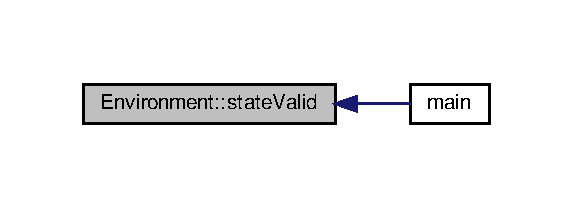
\includegraphics[width=275pt]{class_environment_ad21a790ab0279b0f5b445e1f460dc971_icgraph}
\end{center}
\end{figure}
\mbox{\Hypertarget{class_environment_ad21a790ab0279b0f5b445e1f460dc971}\label{class_environment_ad21a790ab0279b0f5b445e1f460dc971}} 
\index{Environment@{Environment}!state\+Valid@{state\+Valid}}
\index{state\+Valid@{state\+Valid}!Environment@{Environment}}
\subsubsection{\texorpdfstring{state\+Valid()}{stateValid()}\hspace{0.1cm}{\footnotesize\ttfamily [2/2]}}
{\footnotesize\ttfamily bool Environment\+::state\+Valid (\begin{DoxyParamCaption}\item[{const \hyperlink{struct_state}{State} \&}]{s }\end{DoxyParamCaption})\hspace{0.3cm}{\ttfamily [inline]}}



Definition at line 149 of file a\+\_\+star\+\_\+epsilon.\+cpp.



The documentation for this class was generated from the following files\+:\begin{DoxyCompactItemize}
\item 
third\+\_\+party/ecbs/src/\hyperlink{a__star_8cpp}{a\+\_\+star.\+cpp}\item 
third\+\_\+party/ecbs/src/\hyperlink{a__star__epsilon_8cpp}{a\+\_\+star\+\_\+epsilon.\+cpp}\item 
third\+\_\+party/ecbs/src/\hyperlink{cbs_8cpp}{cbs.\+cpp}\item 
third\+\_\+party/ecbs/src/\hyperlink{ecbs_8cpp}{ecbs.\+cpp}\end{DoxyCompactItemize}

\hypertarget{structstd_1_1hash_3_01_edge_constraint_01_4}{}\section{std\+:\+:hash$<$ Edge\+Constraint $>$ Struct Template Reference}
\label{structstd_1_1hash_3_01_edge_constraint_01_4}\index{std\+::hash$<$ Edge\+Constraint $>$@{std\+::hash$<$ Edge\+Constraint $>$}}


{\ttfamily \#include $<$environment.\+hpp$>$}

\subsection*{Public Member Functions}
\begin{DoxyCompactItemize}
\item 
size\+\_\+t \hyperlink{structstd_1_1hash_3_01_edge_constraint_01_4_a3a90f0722b2812ddbc6f12fb0f09e0e7}{operator()} (const \hyperlink{structlib_multi_robot_planning_1_1_edge_constraint}{Edge\+Constraint} \&s) const
\item 
size\+\_\+t \hyperlink{structstd_1_1hash_3_01_edge_constraint_01_4_a3a90f0722b2812ddbc6f12fb0f09e0e7}{operator()} (const \hyperlink{struct_edge_constraint}{Edge\+Constraint} \&s) const
\item 
size\+\_\+t \hyperlink{structstd_1_1hash_3_01_edge_constraint_01_4_a3a90f0722b2812ddbc6f12fb0f09e0e7}{operator()} (const \hyperlink{struct_edge_constraint}{Edge\+Constraint} \&s) const
\end{DoxyCompactItemize}


\subsection{Detailed Description}
\subsubsection*{template$<$$>$\newline
struct std\+::hash$<$ Edge\+Constraint $>$}



Definition at line 192 of file environment.\+hpp.



\subsection{Member Function Documentation}
\mbox{\Hypertarget{structstd_1_1hash_3_01_edge_constraint_01_4_a3a90f0722b2812ddbc6f12fb0f09e0e7}\label{structstd_1_1hash_3_01_edge_constraint_01_4_a3a90f0722b2812ddbc6f12fb0f09e0e7}} 
\index{std\+::hash$<$ Edge\+Constraint $>$@{std\+::hash$<$ Edge\+Constraint $>$}!operator()@{operator()}}
\index{operator()@{operator()}!std\+::hash$<$ Edge\+Constraint $>$@{std\+::hash$<$ Edge\+Constraint $>$}}
\subsubsection{\texorpdfstring{operator()()}{operator()()}\hspace{0.1cm}{\footnotesize\ttfamily [1/3]}}
{\footnotesize\ttfamily size\+\_\+t std\+::hash$<$ \hyperlink{struct_edge_constraint}{Edge\+Constraint} $>$\+::operator() (\begin{DoxyParamCaption}\item[{const \hyperlink{struct_edge_constraint}{Edge\+Constraint} \&}]{s }\end{DoxyParamCaption}) const\hspace{0.3cm}{\ttfamily [inline]}}



Definition at line 184 of file cbs.\+cpp.

\mbox{\Hypertarget{structstd_1_1hash_3_01_edge_constraint_01_4_a3a90f0722b2812ddbc6f12fb0f09e0e7}\label{structstd_1_1hash_3_01_edge_constraint_01_4_a3a90f0722b2812ddbc6f12fb0f09e0e7}} 
\index{std\+::hash$<$ Edge\+Constraint $>$@{std\+::hash$<$ Edge\+Constraint $>$}!operator()@{operator()}}
\index{operator()@{operator()}!std\+::hash$<$ Edge\+Constraint $>$@{std\+::hash$<$ Edge\+Constraint $>$}}
\subsubsection{\texorpdfstring{operator()()}{operator()()}\hspace{0.1cm}{\footnotesize\ttfamily [2/3]}}
{\footnotesize\ttfamily size\+\_\+t std\+::hash$<$ \hyperlink{struct_edge_constraint}{Edge\+Constraint} $>$\+::operator() (\begin{DoxyParamCaption}\item[{const \hyperlink{struct_edge_constraint}{Edge\+Constraint} \&}]{s }\end{DoxyParamCaption}) const\hspace{0.3cm}{\ttfamily [inline]}}



Definition at line 184 of file ecbs.\+cpp.

\mbox{\Hypertarget{structstd_1_1hash_3_01_edge_constraint_01_4_a3a90f0722b2812ddbc6f12fb0f09e0e7}\label{structstd_1_1hash_3_01_edge_constraint_01_4_a3a90f0722b2812ddbc6f12fb0f09e0e7}} 
\index{std\+::hash$<$ Edge\+Constraint $>$@{std\+::hash$<$ Edge\+Constraint $>$}!operator()@{operator()}}
\index{operator()@{operator()}!std\+::hash$<$ Edge\+Constraint $>$@{std\+::hash$<$ Edge\+Constraint $>$}}
\subsubsection{\texorpdfstring{operator()()}{operator()()}\hspace{0.1cm}{\footnotesize\ttfamily [3/3]}}
{\footnotesize\ttfamily size\+\_\+t std\+::hash$<$ \hyperlink{structlib_multi_robot_planning_1_1_edge_constraint}{Edge\+Constraint} $>$\+::operator() (\begin{DoxyParamCaption}\item[{const \hyperlink{structlib_multi_robot_planning_1_1_edge_constraint}{Edge\+Constraint} \&}]{s }\end{DoxyParamCaption}) const\hspace{0.3cm}{\ttfamily [inline]}}



Definition at line 193 of file environment.\+hpp.



The documentation for this struct was generated from the following files\+:\begin{DoxyCompactItemize}
\item 
third\+\_\+party/ecbs/include/\hyperlink{environment_8hpp}{environment.\+hpp}\item 
third\+\_\+party/ecbs/src/\hyperlink{cbs_8cpp}{cbs.\+cpp}\item 
third\+\_\+party/ecbs/src/\hyperlink{ecbs_8cpp}{ecbs.\+cpp}\end{DoxyCompactItemize}

\hypertarget{structstd_1_1hash_3_01_location_01_4}{}\section{std\+:\+:hash$<$ Location $>$ Struct Template Reference}
\label{structstd_1_1hash_3_01_location_01_4}\index{std\+::hash$<$ Location $>$@{std\+::hash$<$ Location $>$}}


{\ttfamily \#include $<$environment.\+hpp$>$}

\subsection*{Public Member Functions}
\begin{DoxyCompactItemize}
\item 
size\+\_\+t \hyperlink{structstd_1_1hash_3_01_location_01_4_a51d2a62300e726c24c2372482698a89b}{operator()} (const \hyperlink{structlib_multi_robot_planning_1_1_location}{Location} \&s) const
\item 
size\+\_\+t \hyperlink{structstd_1_1hash_3_01_location_01_4_a51d2a62300e726c24c2372482698a89b}{operator()} (const \hyperlink{struct_location}{Location} \&s) const
\item 
size\+\_\+t \hyperlink{structstd_1_1hash_3_01_location_01_4_a51d2a62300e726c24c2372482698a89b}{operator()} (const \hyperlink{struct_location}{Location} \&s) const
\end{DoxyCompactItemize}


\subsection{Detailed Description}
\subsubsection*{template$<$$>$\newline
struct std\+::hash$<$ Location $>$}



Definition at line 266 of file environment.\+hpp.



\subsection{Member Function Documentation}
\mbox{\Hypertarget{structstd_1_1hash_3_01_location_01_4_a51d2a62300e726c24c2372482698a89b}\label{structstd_1_1hash_3_01_location_01_4_a51d2a62300e726c24c2372482698a89b}} 
\index{std\+::hash$<$ Location $>$@{std\+::hash$<$ Location $>$}!operator()@{operator()}}
\index{operator()@{operator()}!std\+::hash$<$ Location $>$@{std\+::hash$<$ Location $>$}}
\subsubsection{\texorpdfstring{operator()()}{operator()()}\hspace{0.1cm}{\footnotesize\ttfamily [1/3]}}
{\footnotesize\ttfamily size\+\_\+t std\+::hash$<$ \hyperlink{struct_location}{Location} $>$\+::operator() (\begin{DoxyParamCaption}\item[{const \hyperlink{struct_location}{Location} \&}]{s }\end{DoxyParamCaption}) const\hspace{0.3cm}{\ttfamily [inline]}}



Definition at line 256 of file cbs.\+cpp.

\mbox{\Hypertarget{structstd_1_1hash_3_01_location_01_4_a51d2a62300e726c24c2372482698a89b}\label{structstd_1_1hash_3_01_location_01_4_a51d2a62300e726c24c2372482698a89b}} 
\index{std\+::hash$<$ Location $>$@{std\+::hash$<$ Location $>$}!operator()@{operator()}}
\index{operator()@{operator()}!std\+::hash$<$ Location $>$@{std\+::hash$<$ Location $>$}}
\subsubsection{\texorpdfstring{operator()()}{operator()()}\hspace{0.1cm}{\footnotesize\ttfamily [2/3]}}
{\footnotesize\ttfamily size\+\_\+t std\+::hash$<$ \hyperlink{struct_location}{Location} $>$\+::operator() (\begin{DoxyParamCaption}\item[{const \hyperlink{struct_location}{Location} \&}]{s }\end{DoxyParamCaption}) const\hspace{0.3cm}{\ttfamily [inline]}}



Definition at line 256 of file ecbs.\+cpp.

\mbox{\Hypertarget{structstd_1_1hash_3_01_location_01_4_a51d2a62300e726c24c2372482698a89b}\label{structstd_1_1hash_3_01_location_01_4_a51d2a62300e726c24c2372482698a89b}} 
\index{std\+::hash$<$ Location $>$@{std\+::hash$<$ Location $>$}!operator()@{operator()}}
\index{operator()@{operator()}!std\+::hash$<$ Location $>$@{std\+::hash$<$ Location $>$}}
\subsubsection{\texorpdfstring{operator()()}{operator()()}\hspace{0.1cm}{\footnotesize\ttfamily [3/3]}}
{\footnotesize\ttfamily size\+\_\+t std\+::hash$<$ \hyperlink{structlib_multi_robot_planning_1_1_location}{Location} $>$\+::operator() (\begin{DoxyParamCaption}\item[{const \hyperlink{structlib_multi_robot_planning_1_1_location}{Location} \&}]{s }\end{DoxyParamCaption}) const\hspace{0.3cm}{\ttfamily [inline]}}



Definition at line 267 of file environment.\+hpp.



The documentation for this struct was generated from the following files\+:\begin{DoxyCompactItemize}
\item 
third\+\_\+party/ecbs/include/\hyperlink{environment_8hpp}{environment.\+hpp}\item 
third\+\_\+party/ecbs/src/\hyperlink{cbs_8cpp}{cbs.\+cpp}\item 
third\+\_\+party/ecbs/src/\hyperlink{ecbs_8cpp}{ecbs.\+cpp}\end{DoxyCompactItemize}

\hypertarget{structstd_1_1hash_3_01_state_01_4}{}\section{std\+:\+:hash$<$ State $>$ Struct Template Reference}
\label{structstd_1_1hash_3_01_state_01_4}\index{std\+::hash$<$ State $>$@{std\+::hash$<$ State $>$}}


{\ttfamily \#include $<$environment.\+hpp$>$}

\subsection*{Public Member Functions}
\begin{DoxyCompactItemize}
\item 
size\+\_\+t \hyperlink{structstd_1_1hash_3_01_state_01_4_af7fa7225302eecf4b97ebb57bcaf3b70}{operator()} (const \hyperlink{structlib_multi_robot_planning_1_1_state}{State} \&s) const
\item 
size\+\_\+t \hyperlink{structstd_1_1hash_3_01_state_01_4_af7fa7225302eecf4b97ebb57bcaf3b70}{operator()} (const \hyperlink{struct_state}{State} \&s) const
\item 
size\+\_\+t \hyperlink{structstd_1_1hash_3_01_state_01_4_af7fa7225302eecf4b97ebb57bcaf3b70}{operator()} (const \hyperlink{struct_state}{State} \&s) const
\item 
size\+\_\+t \hyperlink{structstd_1_1hash_3_01_state_01_4_af7fa7225302eecf4b97ebb57bcaf3b70}{operator()} (const \hyperlink{struct_state}{State} \&s) const
\item 
size\+\_\+t \hyperlink{structstd_1_1hash_3_01_state_01_4_af7fa7225302eecf4b97ebb57bcaf3b70}{operator()} (const \hyperlink{struct_state}{State} \&s) const
\end{DoxyCompactItemize}


\subsection{Detailed Description}
\subsubsection*{template$<$$>$\newline
struct std\+::hash$<$ State $>$}



Definition at line 40 of file environment.\+hpp.



\subsection{Member Function Documentation}
\mbox{\Hypertarget{structstd_1_1hash_3_01_state_01_4_af7fa7225302eecf4b97ebb57bcaf3b70}\label{structstd_1_1hash_3_01_state_01_4_af7fa7225302eecf4b97ebb57bcaf3b70}} 
\index{std\+::hash$<$ State $>$@{std\+::hash$<$ State $>$}!operator()@{operator()}}
\index{operator()@{operator()}!std\+::hash$<$ State $>$@{std\+::hash$<$ State $>$}}
\subsubsection{\texorpdfstring{operator()()}{operator()()}\hspace{0.1cm}{\footnotesize\ttfamily [1/5]}}
{\footnotesize\ttfamily size\+\_\+t std\+::hash$<$ \hyperlink{struct_state}{State} $>$\+::operator() (\begin{DoxyParamCaption}\item[{const \hyperlink{struct_state}{State} \&}]{s }\end{DoxyParamCaption}) const\hspace{0.3cm}{\ttfamily [inline]}}



Definition at line 36 of file a\+\_\+star.\+cpp.

\mbox{\Hypertarget{structstd_1_1hash_3_01_state_01_4_af7fa7225302eecf4b97ebb57bcaf3b70}\label{structstd_1_1hash_3_01_state_01_4_af7fa7225302eecf4b97ebb57bcaf3b70}} 
\index{std\+::hash$<$ State $>$@{std\+::hash$<$ State $>$}!operator()@{operator()}}
\index{operator()@{operator()}!std\+::hash$<$ State $>$@{std\+::hash$<$ State $>$}}
\subsubsection{\texorpdfstring{operator()()}{operator()()}\hspace{0.1cm}{\footnotesize\ttfamily [2/5]}}
{\footnotesize\ttfamily size\+\_\+t std\+::hash$<$ \hyperlink{struct_state}{State} $>$\+::operator() (\begin{DoxyParamCaption}\item[{const \hyperlink{struct_state}{State} \&}]{s }\end{DoxyParamCaption}) const\hspace{0.3cm}{\ttfamily [inline]}}



Definition at line 37 of file a\+\_\+star\+\_\+epsilon.\+cpp.

\mbox{\Hypertarget{structstd_1_1hash_3_01_state_01_4_af7fa7225302eecf4b97ebb57bcaf3b70}\label{structstd_1_1hash_3_01_state_01_4_af7fa7225302eecf4b97ebb57bcaf3b70}} 
\index{std\+::hash$<$ State $>$@{std\+::hash$<$ State $>$}!operator()@{operator()}}
\index{operator()@{operator()}!std\+::hash$<$ State $>$@{std\+::hash$<$ State $>$}}
\subsubsection{\texorpdfstring{operator()()}{operator()()}\hspace{0.1cm}{\footnotesize\ttfamily [3/5]}}
{\footnotesize\ttfamily size\+\_\+t std\+::hash$<$ \hyperlink{struct_state}{State} $>$\+::operator() (\begin{DoxyParamCaption}\item[{const \hyperlink{struct_state}{State} \&}]{s }\end{DoxyParamCaption}) const\hspace{0.3cm}{\ttfamily [inline]}}



Definition at line 39 of file cbs.\+cpp.

\mbox{\Hypertarget{structstd_1_1hash_3_01_state_01_4_af7fa7225302eecf4b97ebb57bcaf3b70}\label{structstd_1_1hash_3_01_state_01_4_af7fa7225302eecf4b97ebb57bcaf3b70}} 
\index{std\+::hash$<$ State $>$@{std\+::hash$<$ State $>$}!operator()@{operator()}}
\index{operator()@{operator()}!std\+::hash$<$ State $>$@{std\+::hash$<$ State $>$}}
\subsubsection{\texorpdfstring{operator()()}{operator()()}\hspace{0.1cm}{\footnotesize\ttfamily [4/5]}}
{\footnotesize\ttfamily size\+\_\+t std\+::hash$<$ \hyperlink{struct_state}{State} $>$\+::operator() (\begin{DoxyParamCaption}\item[{const \hyperlink{struct_state}{State} \&}]{s }\end{DoxyParamCaption}) const\hspace{0.3cm}{\ttfamily [inline]}}



Definition at line 39 of file ecbs.\+cpp.

\mbox{\Hypertarget{structstd_1_1hash_3_01_state_01_4_af7fa7225302eecf4b97ebb57bcaf3b70}\label{structstd_1_1hash_3_01_state_01_4_af7fa7225302eecf4b97ebb57bcaf3b70}} 
\index{std\+::hash$<$ State $>$@{std\+::hash$<$ State $>$}!operator()@{operator()}}
\index{operator()@{operator()}!std\+::hash$<$ State $>$@{std\+::hash$<$ State $>$}}
\subsubsection{\texorpdfstring{operator()()}{operator()()}\hspace{0.1cm}{\footnotesize\ttfamily [5/5]}}
{\footnotesize\ttfamily size\+\_\+t std\+::hash$<$ \hyperlink{structlib_multi_robot_planning_1_1_state}{State} $>$\+::operator() (\begin{DoxyParamCaption}\item[{const \hyperlink{structlib_multi_robot_planning_1_1_state}{State} \&}]{s }\end{DoxyParamCaption}) const\hspace{0.3cm}{\ttfamily [inline]}}



Definition at line 41 of file environment.\+hpp.



The documentation for this struct was generated from the following files\+:\begin{DoxyCompactItemize}
\item 
third\+\_\+party/ecbs/include/\hyperlink{environment_8hpp}{environment.\+hpp}\item 
third\+\_\+party/ecbs/src/\hyperlink{a__star_8cpp}{a\+\_\+star.\+cpp}\item 
third\+\_\+party/ecbs/src/\hyperlink{a__star__epsilon_8cpp}{a\+\_\+star\+\_\+epsilon.\+cpp}\item 
third\+\_\+party/ecbs/src/\hyperlink{cbs_8cpp}{cbs.\+cpp}\item 
third\+\_\+party/ecbs/src/\hyperlink{ecbs_8cpp}{ecbs.\+cpp}\end{DoxyCompactItemize}

\hypertarget{structstd_1_1hash_3_01_vertex_constraint_01_4}{}\section{std\+:\+:hash$<$ Vertex\+Constraint $>$ Struct Template Reference}
\label{structstd_1_1hash_3_01_vertex_constraint_01_4}\index{std\+::hash$<$ Vertex\+Constraint $>$@{std\+::hash$<$ Vertex\+Constraint $>$}}


{\ttfamily \#include $<$environment.\+hpp$>$}

\subsection*{Public Member Functions}
\begin{DoxyCompactItemize}
\item 
size\+\_\+t \hyperlink{structstd_1_1hash_3_01_vertex_constraint_01_4_aea9029af41dea6bb20a7a1c8f7e4091c}{operator()} (const \hyperlink{structlib_multi_robot_planning_1_1_vertex_constraint}{Vertex\+Constraint} \&s) const
\item 
size\+\_\+t \hyperlink{structstd_1_1hash_3_01_vertex_constraint_01_4_aea9029af41dea6bb20a7a1c8f7e4091c}{operator()} (const \hyperlink{struct_vertex_constraint}{Vertex\+Constraint} \&s) const
\item 
size\+\_\+t \hyperlink{structstd_1_1hash_3_01_vertex_constraint_01_4_aea9029af41dea6bb20a7a1c8f7e4091c}{operator()} (const \hyperlink{struct_vertex_constraint}{Vertex\+Constraint} \&s) const
\end{DoxyCompactItemize}


\subsection{Detailed Description}
\subsubsection*{template$<$$>$\newline
struct std\+::hash$<$ Vertex\+Constraint $>$}



Definition at line 148 of file environment.\+hpp.



\subsection{Member Function Documentation}
\mbox{\Hypertarget{structstd_1_1hash_3_01_vertex_constraint_01_4_aea9029af41dea6bb20a7a1c8f7e4091c}\label{structstd_1_1hash_3_01_vertex_constraint_01_4_aea9029af41dea6bb20a7a1c8f7e4091c}} 
\index{std\+::hash$<$ Vertex\+Constraint $>$@{std\+::hash$<$ Vertex\+Constraint $>$}!operator()@{operator()}}
\index{operator()@{operator()}!std\+::hash$<$ Vertex\+Constraint $>$@{std\+::hash$<$ Vertex\+Constraint $>$}}
\subsubsection{\texorpdfstring{operator()()}{operator()()}\hspace{0.1cm}{\footnotesize\ttfamily [1/3]}}
{\footnotesize\ttfamily size\+\_\+t std\+::hash$<$ \hyperlink{struct_vertex_constraint}{Vertex\+Constraint} $>$\+::operator() (\begin{DoxyParamCaption}\item[{const \hyperlink{struct_vertex_constraint}{Vertex\+Constraint} \&}]{s }\end{DoxyParamCaption}) const\hspace{0.3cm}{\ttfamily [inline]}}



Definition at line 143 of file cbs.\+cpp.

\mbox{\Hypertarget{structstd_1_1hash_3_01_vertex_constraint_01_4_aea9029af41dea6bb20a7a1c8f7e4091c}\label{structstd_1_1hash_3_01_vertex_constraint_01_4_aea9029af41dea6bb20a7a1c8f7e4091c}} 
\index{std\+::hash$<$ Vertex\+Constraint $>$@{std\+::hash$<$ Vertex\+Constraint $>$}!operator()@{operator()}}
\index{operator()@{operator()}!std\+::hash$<$ Vertex\+Constraint $>$@{std\+::hash$<$ Vertex\+Constraint $>$}}
\subsubsection{\texorpdfstring{operator()()}{operator()()}\hspace{0.1cm}{\footnotesize\ttfamily [2/3]}}
{\footnotesize\ttfamily size\+\_\+t std\+::hash$<$ \hyperlink{struct_vertex_constraint}{Vertex\+Constraint} $>$\+::operator() (\begin{DoxyParamCaption}\item[{const \hyperlink{struct_vertex_constraint}{Vertex\+Constraint} \&}]{s }\end{DoxyParamCaption}) const\hspace{0.3cm}{\ttfamily [inline]}}



Definition at line 143 of file ecbs.\+cpp.

\mbox{\Hypertarget{structstd_1_1hash_3_01_vertex_constraint_01_4_aea9029af41dea6bb20a7a1c8f7e4091c}\label{structstd_1_1hash_3_01_vertex_constraint_01_4_aea9029af41dea6bb20a7a1c8f7e4091c}} 
\index{std\+::hash$<$ Vertex\+Constraint $>$@{std\+::hash$<$ Vertex\+Constraint $>$}!operator()@{operator()}}
\index{operator()@{operator()}!std\+::hash$<$ Vertex\+Constraint $>$@{std\+::hash$<$ Vertex\+Constraint $>$}}
\subsubsection{\texorpdfstring{operator()()}{operator()()}\hspace{0.1cm}{\footnotesize\ttfamily [3/3]}}
{\footnotesize\ttfamily size\+\_\+t std\+::hash$<$ \hyperlink{structlib_multi_robot_planning_1_1_vertex_constraint}{Vertex\+Constraint} $>$\+::operator() (\begin{DoxyParamCaption}\item[{const \hyperlink{structlib_multi_robot_planning_1_1_vertex_constraint}{Vertex\+Constraint} \&}]{s }\end{DoxyParamCaption}) const\hspace{0.3cm}{\ttfamily [inline]}}



Definition at line 149 of file environment.\+hpp.



The documentation for this struct was generated from the following files\+:\begin{DoxyCompactItemize}
\item 
third\+\_\+party/ecbs/include/\hyperlink{environment_8hpp}{environment.\+hpp}\item 
third\+\_\+party/ecbs/src/\hyperlink{cbs_8cpp}{cbs.\+cpp}\item 
third\+\_\+party/ecbs/src/\hyperlink{ecbs_8cpp}{ecbs.\+cpp}\end{DoxyCompactItemize}

\hypertarget{classlib_corridor_gen_1_1_init_traj_planner}{}\section{lib\+Corridor\+Gen\+:\+:Init\+Traj\+Planner Class Reference}
\label{classlib_corridor_gen_1_1_init_traj_planner}\index{lib\+Corridor\+Gen\+::\+Init\+Traj\+Planner@{lib\+Corridor\+Gen\+::\+Init\+Traj\+Planner}}


{\ttfamily \#include $<$init\+\_\+traj\+\_\+planner.\+hpp$>$}



Inheritance diagram for lib\+Corridor\+Gen\+:\+:Init\+Traj\+Planner\+:
\nopagebreak
\begin{figure}[H]
\begin{center}
\leavevmode
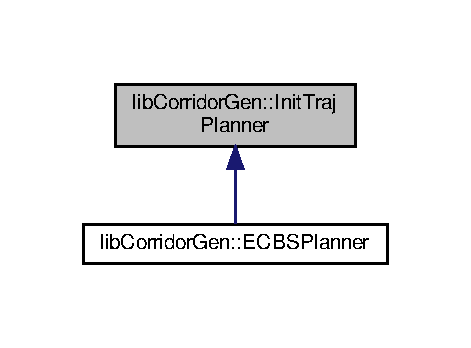
\includegraphics[width=226pt]{classlib_corridor_gen_1_1_init_traj_planner__inherit__graph}
\end{center}
\end{figure}


Collaboration diagram for lib\+Corridor\+Gen\+:\+:Init\+Traj\+Planner\+:
\nopagebreak
\begin{figure}[H]
\begin{center}
\leavevmode
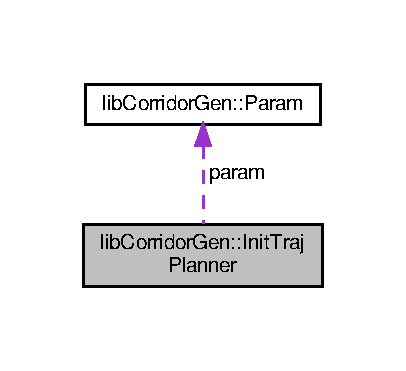
\includegraphics[width=195pt]{classlib_corridor_gen_1_1_init_traj_planner__coll__graph}
\end{center}
\end{figure}
\subsection*{Public Member Functions}
\begin{DoxyCompactItemize}
\item 
virtual bool \hyperlink{classlib_corridor_gen_1_1_init_traj_planner_acfc10a68eddb236a10790c4d92473d99}{update} (bool log)=0
\item 
\hyperlink{classlib_corridor_gen_1_1_init_traj_planner_a0ed77a8c723523592a3c2281dc576b17}{Init\+Traj\+Planner} (std\+::shared\+\_\+ptr$<$ octomap\+::\+Oc\+Tree $>$ \+\_\+octree\+\_\+obj, \hyperlink{classlib_corridor_gen_1_1_param}{Param} \+\_\+param)
\end{DoxyCompactItemize}
\subsection*{Public Attributes}
\begin{DoxyCompactItemize}
\item 
\hyperlink{corridor__common_8hpp_a5505ba29bfa7d0966513cc22822f80f0}{init\+Traj\+\_\+t} \hyperlink{classlib_corridor_gen_1_1_init_traj_planner_a26893ea85eb9d4270ff6920a5c9804a4}{init\+Traj}
\item 
std\+::vector$<$ double $>$ \hyperlink{classlib_corridor_gen_1_1_init_traj_planner_a245efac6cad8f5cac6a09c99dcaf8cbd}{T}
\end{DoxyCompactItemize}
\subsection*{Protected Attributes}
\begin{DoxyCompactItemize}
\item 
std\+::shared\+\_\+ptr$<$ octomap\+::\+Oc\+Tree $>$ \hyperlink{classlib_corridor_gen_1_1_init_traj_planner_a65b1c7c71ee2e55f5e8f7fc1594ba5c9}{octree\+\_\+obj}
\item 
\hyperlink{classlib_corridor_gen_1_1_param}{Param} \hyperlink{classlib_corridor_gen_1_1_init_traj_planner_a2c750ddb7bf244207d43661bda42e1fc}{param}
\item 
double \hyperlink{classlib_corridor_gen_1_1_init_traj_planner_aeb9655c063038a5842fb0b37c52b13dd}{grid\+\_\+x\+\_\+min}
\item 
double \hyperlink{classlib_corridor_gen_1_1_init_traj_planner_aeee7d6390274ab012a2e2158807d0c39}{grid\+\_\+y\+\_\+min}
\item 
double \hyperlink{classlib_corridor_gen_1_1_init_traj_planner_ae02d30b4edf55e3c26a768681403002c}{grid\+\_\+x\+\_\+max}
\item 
double \hyperlink{classlib_corridor_gen_1_1_init_traj_planner_a57a231a6bda58e0d1f281e61c8a9ac5e}{grid\+\_\+y\+\_\+max}
\item 
int \hyperlink{classlib_corridor_gen_1_1_init_traj_planner_a3575a01c82d6d07c08de34219455ef5d}{dimx}
\item 
int \hyperlink{classlib_corridor_gen_1_1_init_traj_planner_ad74c8d5ea299747a09ec949ccb01fa11}{dimy}
\item 
int \hyperlink{classlib_corridor_gen_1_1_init_traj_planner_a3a1684481f8489002dfd1c66c01ccb56}{dimz}
\end{DoxyCompactItemize}


\subsection{Detailed Description}


Definition at line 7 of file init\+\_\+traj\+\_\+planner.\+hpp.



\subsection{Constructor \& Destructor Documentation}
\mbox{\Hypertarget{classlib_corridor_gen_1_1_init_traj_planner_a0ed77a8c723523592a3c2281dc576b17}\label{classlib_corridor_gen_1_1_init_traj_planner_a0ed77a8c723523592a3c2281dc576b17}} 
\index{lib\+Corridor\+Gen\+::\+Init\+Traj\+Planner@{lib\+Corridor\+Gen\+::\+Init\+Traj\+Planner}!Init\+Traj\+Planner@{Init\+Traj\+Planner}}
\index{Init\+Traj\+Planner@{Init\+Traj\+Planner}!lib\+Corridor\+Gen\+::\+Init\+Traj\+Planner@{lib\+Corridor\+Gen\+::\+Init\+Traj\+Planner}}
\subsubsection{\texorpdfstring{Init\+Traj\+Planner()}{InitTrajPlanner()}}
{\footnotesize\ttfamily lib\+Corridor\+Gen\+::\+Init\+Traj\+Planner\+::\+Init\+Traj\+Planner (\begin{DoxyParamCaption}\item[{std\+::shared\+\_\+ptr$<$ octomap\+::\+Oc\+Tree $>$}]{\+\_\+octree\+\_\+obj,  }\item[{\hyperlink{classlib_corridor_gen_1_1_param}{Param}}]{\+\_\+param }\end{DoxyParamCaption})\hspace{0.3cm}{\ttfamily [inline]}}



Definition at line 14 of file init\+\_\+traj\+\_\+planner.\+hpp.



\subsection{Member Function Documentation}
\mbox{\Hypertarget{classlib_corridor_gen_1_1_init_traj_planner_acfc10a68eddb236a10790c4d92473d99}\label{classlib_corridor_gen_1_1_init_traj_planner_acfc10a68eddb236a10790c4d92473d99}} 
\index{lib\+Corridor\+Gen\+::\+Init\+Traj\+Planner@{lib\+Corridor\+Gen\+::\+Init\+Traj\+Planner}!update@{update}}
\index{update@{update}!lib\+Corridor\+Gen\+::\+Init\+Traj\+Planner@{lib\+Corridor\+Gen\+::\+Init\+Traj\+Planner}}
\subsubsection{\texorpdfstring{update()}{update()}}
{\footnotesize\ttfamily virtual bool lib\+Corridor\+Gen\+::\+Init\+Traj\+Planner\+::update (\begin{DoxyParamCaption}\item[{bool}]{log }\end{DoxyParamCaption})\hspace{0.3cm}{\ttfamily [pure virtual]}}



Implemented in \hyperlink{classlib_corridor_gen_1_1_e_c_b_s_planner_a0d4c5855c02228c677b3d2d89c10740c}{lib\+Corridor\+Gen\+::\+E\+C\+B\+S\+Planner}.



\subsection{Member Data Documentation}
\mbox{\Hypertarget{classlib_corridor_gen_1_1_init_traj_planner_a3575a01c82d6d07c08de34219455ef5d}\label{classlib_corridor_gen_1_1_init_traj_planner_a3575a01c82d6d07c08de34219455ef5d}} 
\index{lib\+Corridor\+Gen\+::\+Init\+Traj\+Planner@{lib\+Corridor\+Gen\+::\+Init\+Traj\+Planner}!dimx@{dimx}}
\index{dimx@{dimx}!lib\+Corridor\+Gen\+::\+Init\+Traj\+Planner@{lib\+Corridor\+Gen\+::\+Init\+Traj\+Planner}}
\subsubsection{\texorpdfstring{dimx}{dimx}}
{\footnotesize\ttfamily int lib\+Corridor\+Gen\+::\+Init\+Traj\+Planner\+::dimx\hspace{0.3cm}{\ttfamily [protected]}}



Definition at line 34 of file init\+\_\+traj\+\_\+planner.\+hpp.

\mbox{\Hypertarget{classlib_corridor_gen_1_1_init_traj_planner_ad74c8d5ea299747a09ec949ccb01fa11}\label{classlib_corridor_gen_1_1_init_traj_planner_ad74c8d5ea299747a09ec949ccb01fa11}} 
\index{lib\+Corridor\+Gen\+::\+Init\+Traj\+Planner@{lib\+Corridor\+Gen\+::\+Init\+Traj\+Planner}!dimy@{dimy}}
\index{dimy@{dimy}!lib\+Corridor\+Gen\+::\+Init\+Traj\+Planner@{lib\+Corridor\+Gen\+::\+Init\+Traj\+Planner}}
\subsubsection{\texorpdfstring{dimy}{dimy}}
{\footnotesize\ttfamily int lib\+Corridor\+Gen\+::\+Init\+Traj\+Planner\+::dimy\hspace{0.3cm}{\ttfamily [protected]}}



Definition at line 34 of file init\+\_\+traj\+\_\+planner.\+hpp.

\mbox{\Hypertarget{classlib_corridor_gen_1_1_init_traj_planner_a3a1684481f8489002dfd1c66c01ccb56}\label{classlib_corridor_gen_1_1_init_traj_planner_a3a1684481f8489002dfd1c66c01ccb56}} 
\index{lib\+Corridor\+Gen\+::\+Init\+Traj\+Planner@{lib\+Corridor\+Gen\+::\+Init\+Traj\+Planner}!dimz@{dimz}}
\index{dimz@{dimz}!lib\+Corridor\+Gen\+::\+Init\+Traj\+Planner@{lib\+Corridor\+Gen\+::\+Init\+Traj\+Planner}}
\subsubsection{\texorpdfstring{dimz}{dimz}}
{\footnotesize\ttfamily int lib\+Corridor\+Gen\+::\+Init\+Traj\+Planner\+::dimz\hspace{0.3cm}{\ttfamily [protected]}}



Definition at line 34 of file init\+\_\+traj\+\_\+planner.\+hpp.

\mbox{\Hypertarget{classlib_corridor_gen_1_1_init_traj_planner_ae02d30b4edf55e3c26a768681403002c}\label{classlib_corridor_gen_1_1_init_traj_planner_ae02d30b4edf55e3c26a768681403002c}} 
\index{lib\+Corridor\+Gen\+::\+Init\+Traj\+Planner@{lib\+Corridor\+Gen\+::\+Init\+Traj\+Planner}!grid\+\_\+x\+\_\+max@{grid\+\_\+x\+\_\+max}}
\index{grid\+\_\+x\+\_\+max@{grid\+\_\+x\+\_\+max}!lib\+Corridor\+Gen\+::\+Init\+Traj\+Planner@{lib\+Corridor\+Gen\+::\+Init\+Traj\+Planner}}
\subsubsection{\texorpdfstring{grid\+\_\+x\+\_\+max}{grid\_x\_max}}
{\footnotesize\ttfamily double lib\+Corridor\+Gen\+::\+Init\+Traj\+Planner\+::grid\+\_\+x\+\_\+max\hspace{0.3cm}{\ttfamily [protected]}}



Definition at line 33 of file init\+\_\+traj\+\_\+planner.\+hpp.

\mbox{\Hypertarget{classlib_corridor_gen_1_1_init_traj_planner_aeb9655c063038a5842fb0b37c52b13dd}\label{classlib_corridor_gen_1_1_init_traj_planner_aeb9655c063038a5842fb0b37c52b13dd}} 
\index{lib\+Corridor\+Gen\+::\+Init\+Traj\+Planner@{lib\+Corridor\+Gen\+::\+Init\+Traj\+Planner}!grid\+\_\+x\+\_\+min@{grid\+\_\+x\+\_\+min}}
\index{grid\+\_\+x\+\_\+min@{grid\+\_\+x\+\_\+min}!lib\+Corridor\+Gen\+::\+Init\+Traj\+Planner@{lib\+Corridor\+Gen\+::\+Init\+Traj\+Planner}}
\subsubsection{\texorpdfstring{grid\+\_\+x\+\_\+min}{grid\_x\_min}}
{\footnotesize\ttfamily double lib\+Corridor\+Gen\+::\+Init\+Traj\+Planner\+::grid\+\_\+x\+\_\+min\hspace{0.3cm}{\ttfamily [protected]}}



Definition at line 33 of file init\+\_\+traj\+\_\+planner.\+hpp.

\mbox{\Hypertarget{classlib_corridor_gen_1_1_init_traj_planner_a57a231a6bda58e0d1f281e61c8a9ac5e}\label{classlib_corridor_gen_1_1_init_traj_planner_a57a231a6bda58e0d1f281e61c8a9ac5e}} 
\index{lib\+Corridor\+Gen\+::\+Init\+Traj\+Planner@{lib\+Corridor\+Gen\+::\+Init\+Traj\+Planner}!grid\+\_\+y\+\_\+max@{grid\+\_\+y\+\_\+max}}
\index{grid\+\_\+y\+\_\+max@{grid\+\_\+y\+\_\+max}!lib\+Corridor\+Gen\+::\+Init\+Traj\+Planner@{lib\+Corridor\+Gen\+::\+Init\+Traj\+Planner}}
\subsubsection{\texorpdfstring{grid\+\_\+y\+\_\+max}{grid\_y\_max}}
{\footnotesize\ttfamily double lib\+Corridor\+Gen\+::\+Init\+Traj\+Planner\+::grid\+\_\+y\+\_\+max\hspace{0.3cm}{\ttfamily [protected]}}



Definition at line 33 of file init\+\_\+traj\+\_\+planner.\+hpp.

\mbox{\Hypertarget{classlib_corridor_gen_1_1_init_traj_planner_aeee7d6390274ab012a2e2158807d0c39}\label{classlib_corridor_gen_1_1_init_traj_planner_aeee7d6390274ab012a2e2158807d0c39}} 
\index{lib\+Corridor\+Gen\+::\+Init\+Traj\+Planner@{lib\+Corridor\+Gen\+::\+Init\+Traj\+Planner}!grid\+\_\+y\+\_\+min@{grid\+\_\+y\+\_\+min}}
\index{grid\+\_\+y\+\_\+min@{grid\+\_\+y\+\_\+min}!lib\+Corridor\+Gen\+::\+Init\+Traj\+Planner@{lib\+Corridor\+Gen\+::\+Init\+Traj\+Planner}}
\subsubsection{\texorpdfstring{grid\+\_\+y\+\_\+min}{grid\_y\_min}}
{\footnotesize\ttfamily double lib\+Corridor\+Gen\+::\+Init\+Traj\+Planner\+::grid\+\_\+y\+\_\+min\hspace{0.3cm}{\ttfamily [protected]}}



Definition at line 33 of file init\+\_\+traj\+\_\+planner.\+hpp.

\mbox{\Hypertarget{classlib_corridor_gen_1_1_init_traj_planner_a26893ea85eb9d4270ff6920a5c9804a4}\label{classlib_corridor_gen_1_1_init_traj_planner_a26893ea85eb9d4270ff6920a5c9804a4}} 
\index{lib\+Corridor\+Gen\+::\+Init\+Traj\+Planner@{lib\+Corridor\+Gen\+::\+Init\+Traj\+Planner}!init\+Traj@{init\+Traj}}
\index{init\+Traj@{init\+Traj}!lib\+Corridor\+Gen\+::\+Init\+Traj\+Planner@{lib\+Corridor\+Gen\+::\+Init\+Traj\+Planner}}
\subsubsection{\texorpdfstring{init\+Traj}{initTraj}}
{\footnotesize\ttfamily \hyperlink{corridor__common_8hpp_a5505ba29bfa7d0966513cc22822f80f0}{init\+Traj\+\_\+t} lib\+Corridor\+Gen\+::\+Init\+Traj\+Planner\+::init\+Traj}



Definition at line 9 of file init\+\_\+traj\+\_\+planner.\+hpp.

\mbox{\Hypertarget{classlib_corridor_gen_1_1_init_traj_planner_a65b1c7c71ee2e55f5e8f7fc1594ba5c9}\label{classlib_corridor_gen_1_1_init_traj_planner_a65b1c7c71ee2e55f5e8f7fc1594ba5c9}} 
\index{lib\+Corridor\+Gen\+::\+Init\+Traj\+Planner@{lib\+Corridor\+Gen\+::\+Init\+Traj\+Planner}!octree\+\_\+obj@{octree\+\_\+obj}}
\index{octree\+\_\+obj@{octree\+\_\+obj}!lib\+Corridor\+Gen\+::\+Init\+Traj\+Planner@{lib\+Corridor\+Gen\+::\+Init\+Traj\+Planner}}
\subsubsection{\texorpdfstring{octree\+\_\+obj}{octree\_obj}}
{\footnotesize\ttfamily std\+::shared\+\_\+ptr$<$octomap\+::\+Oc\+Tree$>$ lib\+Corridor\+Gen\+::\+Init\+Traj\+Planner\+::octree\+\_\+obj\hspace{0.3cm}{\ttfamily [protected]}}



Definition at line 30 of file init\+\_\+traj\+\_\+planner.\+hpp.

\mbox{\Hypertarget{classlib_corridor_gen_1_1_init_traj_planner_a2c750ddb7bf244207d43661bda42e1fc}\label{classlib_corridor_gen_1_1_init_traj_planner_a2c750ddb7bf244207d43661bda42e1fc}} 
\index{lib\+Corridor\+Gen\+::\+Init\+Traj\+Planner@{lib\+Corridor\+Gen\+::\+Init\+Traj\+Planner}!param@{param}}
\index{param@{param}!lib\+Corridor\+Gen\+::\+Init\+Traj\+Planner@{lib\+Corridor\+Gen\+::\+Init\+Traj\+Planner}}
\subsubsection{\texorpdfstring{param}{param}}
{\footnotesize\ttfamily \hyperlink{classlib_corridor_gen_1_1_param}{Param} lib\+Corridor\+Gen\+::\+Init\+Traj\+Planner\+::param\hspace{0.3cm}{\ttfamily [protected]}}



Definition at line 31 of file init\+\_\+traj\+\_\+planner.\+hpp.

\mbox{\Hypertarget{classlib_corridor_gen_1_1_init_traj_planner_a245efac6cad8f5cac6a09c99dcaf8cbd}\label{classlib_corridor_gen_1_1_init_traj_planner_a245efac6cad8f5cac6a09c99dcaf8cbd}} 
\index{lib\+Corridor\+Gen\+::\+Init\+Traj\+Planner@{lib\+Corridor\+Gen\+::\+Init\+Traj\+Planner}!T@{T}}
\index{T@{T}!lib\+Corridor\+Gen\+::\+Init\+Traj\+Planner@{lib\+Corridor\+Gen\+::\+Init\+Traj\+Planner}}
\subsubsection{\texorpdfstring{T}{T}}
{\footnotesize\ttfamily std\+::vector$<$double$>$ lib\+Corridor\+Gen\+::\+Init\+Traj\+Planner\+::T}



Definition at line 10 of file init\+\_\+traj\+\_\+planner.\+hpp.



The documentation for this class was generated from the following file\+:\begin{DoxyCompactItemize}
\item 
include/\hyperlink{init__traj__planner_8hpp}{init\+\_\+traj\+\_\+planner.\+hpp}\end{DoxyCompactItemize}

\hypertarget{structlib_multi_robot_planning_1_1_location}{}\section{lib\+Multi\+Robot\+Planning\+:\+:Location Struct Reference}
\label{structlib_multi_robot_planning_1_1_location}\index{lib\+Multi\+Robot\+Planning\+::\+Location@{lib\+Multi\+Robot\+Planning\+::\+Location}}


{\ttfamily \#include $<$environment.\+hpp$>$}

\subsection*{Public Member Functions}
\begin{DoxyCompactItemize}
\item 
\hyperlink{structlib_multi_robot_planning_1_1_location_a575f4c2a0b65829873bee62ab5a5ad96}{Location} (int \hyperlink{structlib_multi_robot_planning_1_1_location_a8b9baca7fdc69a97d8071666af608f82}{x}, int \hyperlink{structlib_multi_robot_planning_1_1_location_a83d2a4d9d01f2c12e2a567a86ca3893a}{y}, int \hyperlink{structlib_multi_robot_planning_1_1_location_a6c016b7c0360b6dee839189d91fdfd72}{z})
\item 
bool \hyperlink{structlib_multi_robot_planning_1_1_location_abe04a4c39f478d6dbfdbbb12fe70253a}{operator$<$} (const \hyperlink{structlib_multi_robot_planning_1_1_location}{Location} \&other) const
\item 
bool \hyperlink{structlib_multi_robot_planning_1_1_location_a2f795f653c6e0a2943eff4b8f42fe5fc}{operator==} (const \hyperlink{structlib_multi_robot_planning_1_1_location}{Location} \&other) const
\end{DoxyCompactItemize}
\subsection*{Public Attributes}
\begin{DoxyCompactItemize}
\item 
int \hyperlink{structlib_multi_robot_planning_1_1_location_a8b9baca7fdc69a97d8071666af608f82}{x}
\item 
int \hyperlink{structlib_multi_robot_planning_1_1_location_a83d2a4d9d01f2c12e2a567a86ca3893a}{y}
\item 
int \hyperlink{structlib_multi_robot_planning_1_1_location_a6c016b7c0360b6dee839189d91fdfd72}{z}
\end{DoxyCompactItemize}
\subsection*{Friends}
\begin{DoxyCompactItemize}
\item 
std\+::ostream \& \hyperlink{structlib_multi_robot_planning_1_1_location_a80d23d3abaf3e34d1cb5202feb05f385}{operator$<$$<$} (std\+::ostream \&os, const \hyperlink{structlib_multi_robot_planning_1_1_location}{Location} \&c)
\end{DoxyCompactItemize}


\subsection{Detailed Description}


Definition at line 244 of file environment.\+hpp.



\subsection{Constructor \& Destructor Documentation}
\mbox{\Hypertarget{structlib_multi_robot_planning_1_1_location_a575f4c2a0b65829873bee62ab5a5ad96}\label{structlib_multi_robot_planning_1_1_location_a575f4c2a0b65829873bee62ab5a5ad96}} 
\index{lib\+Multi\+Robot\+Planning\+::\+Location@{lib\+Multi\+Robot\+Planning\+::\+Location}!Location@{Location}}
\index{Location@{Location}!lib\+Multi\+Robot\+Planning\+::\+Location@{lib\+Multi\+Robot\+Planning\+::\+Location}}
\subsubsection{\texorpdfstring{Location()}{Location()}}
{\footnotesize\ttfamily lib\+Multi\+Robot\+Planning\+::\+Location\+::\+Location (\begin{DoxyParamCaption}\item[{int}]{x,  }\item[{int}]{y,  }\item[{int}]{z }\end{DoxyParamCaption})\hspace{0.3cm}{\ttfamily [inline]}}



Definition at line 245 of file environment.\+hpp.



\subsection{Member Function Documentation}
\mbox{\Hypertarget{structlib_multi_robot_planning_1_1_location_abe04a4c39f478d6dbfdbbb12fe70253a}\label{structlib_multi_robot_planning_1_1_location_abe04a4c39f478d6dbfdbbb12fe70253a}} 
\index{lib\+Multi\+Robot\+Planning\+::\+Location@{lib\+Multi\+Robot\+Planning\+::\+Location}!operator$<$@{operator$<$}}
\index{operator$<$@{operator$<$}!lib\+Multi\+Robot\+Planning\+::\+Location@{lib\+Multi\+Robot\+Planning\+::\+Location}}
\subsubsection{\texorpdfstring{operator$<$()}{operator<()}}
{\footnotesize\ttfamily bool lib\+Multi\+Robot\+Planning\+::\+Location\+::operator$<$ (\begin{DoxyParamCaption}\item[{const \hyperlink{structlib_multi_robot_planning_1_1_location}{Location} \&}]{other }\end{DoxyParamCaption}) const\hspace{0.3cm}{\ttfamily [inline]}}



Definition at line 251 of file environment.\+hpp.

\mbox{\Hypertarget{structlib_multi_robot_planning_1_1_location_a2f795f653c6e0a2943eff4b8f42fe5fc}\label{structlib_multi_robot_planning_1_1_location_a2f795f653c6e0a2943eff4b8f42fe5fc}} 
\index{lib\+Multi\+Robot\+Planning\+::\+Location@{lib\+Multi\+Robot\+Planning\+::\+Location}!operator==@{operator==}}
\index{operator==@{operator==}!lib\+Multi\+Robot\+Planning\+::\+Location@{lib\+Multi\+Robot\+Planning\+::\+Location}}
\subsubsection{\texorpdfstring{operator==()}{operator==()}}
{\footnotesize\ttfamily bool lib\+Multi\+Robot\+Planning\+::\+Location\+::operator== (\begin{DoxyParamCaption}\item[{const \hyperlink{structlib_multi_robot_planning_1_1_location}{Location} \&}]{other }\end{DoxyParamCaption}) const\hspace{0.3cm}{\ttfamily [inline]}}



Definition at line 255 of file environment.\+hpp.



\subsection{Friends And Related Function Documentation}
\mbox{\Hypertarget{structlib_multi_robot_planning_1_1_location_a80d23d3abaf3e34d1cb5202feb05f385}\label{structlib_multi_robot_planning_1_1_location_a80d23d3abaf3e34d1cb5202feb05f385}} 
\index{lib\+Multi\+Robot\+Planning\+::\+Location@{lib\+Multi\+Robot\+Planning\+::\+Location}!operator$<$$<$@{operator$<$$<$}}
\index{operator$<$$<$@{operator$<$$<$}!lib\+Multi\+Robot\+Planning\+::\+Location@{lib\+Multi\+Robot\+Planning\+::\+Location}}
\subsubsection{\texorpdfstring{operator$<$$<$}{operator<<}}
{\footnotesize\ttfamily std\+::ostream\& operator$<$$<$ (\begin{DoxyParamCaption}\item[{std\+::ostream \&}]{os,  }\item[{const \hyperlink{structlib_multi_robot_planning_1_1_location}{Location} \&}]{c }\end{DoxyParamCaption})\hspace{0.3cm}{\ttfamily [friend]}}



Definition at line 259 of file environment.\+hpp.



\subsection{Member Data Documentation}
\mbox{\Hypertarget{structlib_multi_robot_planning_1_1_location_a8b9baca7fdc69a97d8071666af608f82}\label{structlib_multi_robot_planning_1_1_location_a8b9baca7fdc69a97d8071666af608f82}} 
\index{lib\+Multi\+Robot\+Planning\+::\+Location@{lib\+Multi\+Robot\+Planning\+::\+Location}!x@{x}}
\index{x@{x}!lib\+Multi\+Robot\+Planning\+::\+Location@{lib\+Multi\+Robot\+Planning\+::\+Location}}
\subsubsection{\texorpdfstring{x}{x}}
{\footnotesize\ttfamily int lib\+Multi\+Robot\+Planning\+::\+Location\+::x}



Definition at line 247 of file environment.\+hpp.

\mbox{\Hypertarget{structlib_multi_robot_planning_1_1_location_a83d2a4d9d01f2c12e2a567a86ca3893a}\label{structlib_multi_robot_planning_1_1_location_a83d2a4d9d01f2c12e2a567a86ca3893a}} 
\index{lib\+Multi\+Robot\+Planning\+::\+Location@{lib\+Multi\+Robot\+Planning\+::\+Location}!y@{y}}
\index{y@{y}!lib\+Multi\+Robot\+Planning\+::\+Location@{lib\+Multi\+Robot\+Planning\+::\+Location}}
\subsubsection{\texorpdfstring{y}{y}}
{\footnotesize\ttfamily int lib\+Multi\+Robot\+Planning\+::\+Location\+::y}



Definition at line 248 of file environment.\+hpp.

\mbox{\Hypertarget{structlib_multi_robot_planning_1_1_location_a6c016b7c0360b6dee839189d91fdfd72}\label{structlib_multi_robot_planning_1_1_location_a6c016b7c0360b6dee839189d91fdfd72}} 
\index{lib\+Multi\+Robot\+Planning\+::\+Location@{lib\+Multi\+Robot\+Planning\+::\+Location}!z@{z}}
\index{z@{z}!lib\+Multi\+Robot\+Planning\+::\+Location@{lib\+Multi\+Robot\+Planning\+::\+Location}}
\subsubsection{\texorpdfstring{z}{z}}
{\footnotesize\ttfamily int lib\+Multi\+Robot\+Planning\+::\+Location\+::z}



Definition at line 249 of file environment.\+hpp.



The documentation for this struct was generated from the following file\+:\begin{DoxyCompactItemize}
\item 
third\+\_\+party/ecbs/include/\hyperlink{environment_8hpp}{environment.\+hpp}\end{DoxyCompactItemize}

\hypertarget{struct_location}{}\section{Location Struct Reference}
\label{struct_location}\index{Location@{Location}}
\subsection*{Public Member Functions}
\begin{DoxyCompactItemize}
\item 
\hyperlink{struct_location_ada7ef731cfa1f39a6512b3e6eecf434d}{Location} (int \hyperlink{struct_location_aea76eebc474e30c04c53e5f03c6749e3}{x}, int \hyperlink{struct_location_a307809776b981810147af56d9304e273}{y}, int \hyperlink{struct_location_ad46e606795ee67a3775a53da49b37284}{z})
\item 
bool \hyperlink{struct_location_af22acefb6d1dd7de7482915b1c2eae5d}{operator$<$} (const \hyperlink{struct_location}{Location} \&other) const
\item 
bool \hyperlink{struct_location_a0c99c1e65cc6607121da4abdb4894b74}{operator==} (const \hyperlink{struct_location}{Location} \&other) const
\item 
\hyperlink{struct_location_ada7ef731cfa1f39a6512b3e6eecf434d}{Location} (int \hyperlink{struct_location_aea76eebc474e30c04c53e5f03c6749e3}{x}, int \hyperlink{struct_location_a307809776b981810147af56d9304e273}{y}, int \hyperlink{struct_location_ad46e606795ee67a3775a53da49b37284}{z})
\item 
bool \hyperlink{struct_location_af22acefb6d1dd7de7482915b1c2eae5d}{operator$<$} (const \hyperlink{struct_location}{Location} \&other) const
\item 
bool \hyperlink{struct_location_a0c99c1e65cc6607121da4abdb4894b74}{operator==} (const \hyperlink{struct_location}{Location} \&other) const
\end{DoxyCompactItemize}
\subsection*{Public Attributes}
\begin{DoxyCompactItemize}
\item 
int \hyperlink{struct_location_aea76eebc474e30c04c53e5f03c6749e3}{x}
\item 
int \hyperlink{struct_location_a307809776b981810147af56d9304e273}{y}
\item 
int \hyperlink{struct_location_ad46e606795ee67a3775a53da49b37284}{z}
\end{DoxyCompactItemize}
\subsection*{Friends}
\begin{DoxyCompactItemize}
\item 
std\+::ostream \& \hyperlink{struct_location_a80d23d3abaf3e34d1cb5202feb05f385}{operator$<$$<$} (std\+::ostream \&os, const \hyperlink{struct_location}{Location} \&c)
\item 
std\+::ostream \& \hyperlink{struct_location_a80d23d3abaf3e34d1cb5202feb05f385}{operator$<$$<$} (std\+::ostream \&os, const \hyperlink{struct_location}{Location} \&c)
\end{DoxyCompactItemize}


\subsection{Detailed Description}


Definition at line 234 of file cbs.\+cpp.



\subsection{Constructor \& Destructor Documentation}
\mbox{\Hypertarget{struct_location_ada7ef731cfa1f39a6512b3e6eecf434d}\label{struct_location_ada7ef731cfa1f39a6512b3e6eecf434d}} 
\index{Location@{Location}!Location@{Location}}
\index{Location@{Location}!Location@{Location}}
\subsubsection{\texorpdfstring{Location()}{Location()}\hspace{0.1cm}{\footnotesize\ttfamily [1/2]}}
{\footnotesize\ttfamily Location\+::\+Location (\begin{DoxyParamCaption}\item[{int}]{x,  }\item[{int}]{y,  }\item[{int}]{z }\end{DoxyParamCaption})\hspace{0.3cm}{\ttfamily [inline]}}



Definition at line 235 of file cbs.\+cpp.

\mbox{\Hypertarget{struct_location_ada7ef731cfa1f39a6512b3e6eecf434d}\label{struct_location_ada7ef731cfa1f39a6512b3e6eecf434d}} 
\index{Location@{Location}!Location@{Location}}
\index{Location@{Location}!Location@{Location}}
\subsubsection{\texorpdfstring{Location()}{Location()}\hspace{0.1cm}{\footnotesize\ttfamily [2/2]}}
{\footnotesize\ttfamily Location\+::\+Location (\begin{DoxyParamCaption}\item[{int}]{x,  }\item[{int}]{y,  }\item[{int}]{z }\end{DoxyParamCaption})\hspace{0.3cm}{\ttfamily [inline]}}



Definition at line 235 of file ecbs.\+cpp.



\subsection{Member Function Documentation}
\mbox{\Hypertarget{struct_location_af22acefb6d1dd7de7482915b1c2eae5d}\label{struct_location_af22acefb6d1dd7de7482915b1c2eae5d}} 
\index{Location@{Location}!operator$<$@{operator$<$}}
\index{operator$<$@{operator$<$}!Location@{Location}}
\subsubsection{\texorpdfstring{operator$<$()}{operator<()}\hspace{0.1cm}{\footnotesize\ttfamily [1/2]}}
{\footnotesize\ttfamily bool Location\+::operator$<$ (\begin{DoxyParamCaption}\item[{const \hyperlink{struct_location}{Location} \&}]{other }\end{DoxyParamCaption}) const\hspace{0.3cm}{\ttfamily [inline]}}



Definition at line 240 of file cbs.\+cpp.

\mbox{\Hypertarget{struct_location_af22acefb6d1dd7de7482915b1c2eae5d}\label{struct_location_af22acefb6d1dd7de7482915b1c2eae5d}} 
\index{Location@{Location}!operator$<$@{operator$<$}}
\index{operator$<$@{operator$<$}!Location@{Location}}
\subsubsection{\texorpdfstring{operator$<$()}{operator<()}\hspace{0.1cm}{\footnotesize\ttfamily [2/2]}}
{\footnotesize\ttfamily bool Location\+::operator$<$ (\begin{DoxyParamCaption}\item[{const \hyperlink{struct_location}{Location} \&}]{other }\end{DoxyParamCaption}) const\hspace{0.3cm}{\ttfamily [inline]}}



Definition at line 240 of file ecbs.\+cpp.

\mbox{\Hypertarget{struct_location_a0c99c1e65cc6607121da4abdb4894b74}\label{struct_location_a0c99c1e65cc6607121da4abdb4894b74}} 
\index{Location@{Location}!operator==@{operator==}}
\index{operator==@{operator==}!Location@{Location}}
\subsubsection{\texorpdfstring{operator==()}{operator==()}\hspace{0.1cm}{\footnotesize\ttfamily [1/2]}}
{\footnotesize\ttfamily bool Location\+::operator== (\begin{DoxyParamCaption}\item[{const \hyperlink{struct_location}{Location} \&}]{other }\end{DoxyParamCaption}) const\hspace{0.3cm}{\ttfamily [inline]}}



Definition at line 244 of file ecbs.\+cpp.

\mbox{\Hypertarget{struct_location_a0c99c1e65cc6607121da4abdb4894b74}\label{struct_location_a0c99c1e65cc6607121da4abdb4894b74}} 
\index{Location@{Location}!operator==@{operator==}}
\index{operator==@{operator==}!Location@{Location}}
\subsubsection{\texorpdfstring{operator==()}{operator==()}\hspace{0.1cm}{\footnotesize\ttfamily [2/2]}}
{\footnotesize\ttfamily bool Location\+::operator== (\begin{DoxyParamCaption}\item[{const \hyperlink{struct_location}{Location} \&}]{other }\end{DoxyParamCaption}) const\hspace{0.3cm}{\ttfamily [inline]}}



Definition at line 244 of file cbs.\+cpp.



\subsection{Friends And Related Function Documentation}
\mbox{\Hypertarget{struct_location_a80d23d3abaf3e34d1cb5202feb05f385}\label{struct_location_a80d23d3abaf3e34d1cb5202feb05f385}} 
\index{Location@{Location}!operator$<$$<$@{operator$<$$<$}}
\index{operator$<$$<$@{operator$<$$<$}!Location@{Location}}
\subsubsection{\texorpdfstring{operator$<$$<$}{operator<<}\hspace{0.1cm}{\footnotesize\ttfamily [1/2]}}
{\footnotesize\ttfamily std\+::ostream\& operator$<$$<$ (\begin{DoxyParamCaption}\item[{std\+::ostream \&}]{os,  }\item[{const \hyperlink{struct_location}{Location} \&}]{c }\end{DoxyParamCaption})\hspace{0.3cm}{\ttfamily [friend]}}



Definition at line 248 of file cbs.\+cpp.

\mbox{\Hypertarget{struct_location_a80d23d3abaf3e34d1cb5202feb05f385}\label{struct_location_a80d23d3abaf3e34d1cb5202feb05f385}} 
\index{Location@{Location}!operator$<$$<$@{operator$<$$<$}}
\index{operator$<$$<$@{operator$<$$<$}!Location@{Location}}
\subsubsection{\texorpdfstring{operator$<$$<$}{operator<<}\hspace{0.1cm}{\footnotesize\ttfamily [2/2]}}
{\footnotesize\ttfamily std\+::ostream\& operator$<$$<$ (\begin{DoxyParamCaption}\item[{std\+::ostream \&}]{os,  }\item[{const \hyperlink{struct_location}{Location} \&}]{c }\end{DoxyParamCaption})\hspace{0.3cm}{\ttfamily [friend]}}



Definition at line 248 of file ecbs.\+cpp.



\subsection{Member Data Documentation}
\mbox{\Hypertarget{struct_location_aea76eebc474e30c04c53e5f03c6749e3}\label{struct_location_aea76eebc474e30c04c53e5f03c6749e3}} 
\index{Location@{Location}!x@{x}}
\index{x@{x}!Location@{Location}}
\subsubsection{\texorpdfstring{x}{x}}
{\footnotesize\ttfamily int Location\+::x}



Definition at line 236 of file cbs.\+cpp.

\mbox{\Hypertarget{struct_location_a307809776b981810147af56d9304e273}\label{struct_location_a307809776b981810147af56d9304e273}} 
\index{Location@{Location}!y@{y}}
\index{y@{y}!Location@{Location}}
\subsubsection{\texorpdfstring{y}{y}}
{\footnotesize\ttfamily int Location\+::y}



Definition at line 237 of file cbs.\+cpp.

\mbox{\Hypertarget{struct_location_ad46e606795ee67a3775a53da49b37284}\label{struct_location_ad46e606795ee67a3775a53da49b37284}} 
\index{Location@{Location}!z@{z}}
\index{z@{z}!Location@{Location}}
\subsubsection{\texorpdfstring{z}{z}}
{\footnotesize\ttfamily int Location\+::z}



Definition at line 238 of file cbs.\+cpp.



The documentation for this struct was generated from the following files\+:\begin{DoxyCompactItemize}
\item 
third\+\_\+party/ecbs/src/\hyperlink{cbs_8cpp}{cbs.\+cpp}\item 
third\+\_\+party/ecbs/src/\hyperlink{ecbs_8cpp}{ecbs.\+cpp}\end{DoxyCompactItemize}

\hypertarget{structlib_multi_robot_planning_1_1_neighbor}{}\section{lib\+Multi\+Robot\+Planning\+:\+:Neighbor$<$ State, Action, Cost $>$ Struct Template Reference}
\label{structlib_multi_robot_planning_1_1_neighbor}\index{lib\+Multi\+Robot\+Planning\+::\+Neighbor$<$ State, Action, Cost $>$@{lib\+Multi\+Robot\+Planning\+::\+Neighbor$<$ State, Action, Cost $>$}}


Represents state transations.  




{\ttfamily \#include $<$neighbor.\+hpp$>$}



Collaboration diagram for lib\+Multi\+Robot\+Planning\+:\+:Neighbor$<$ State, Action, Cost $>$\+:
\nopagebreak
\begin{figure}[H]
\begin{center}
\leavevmode
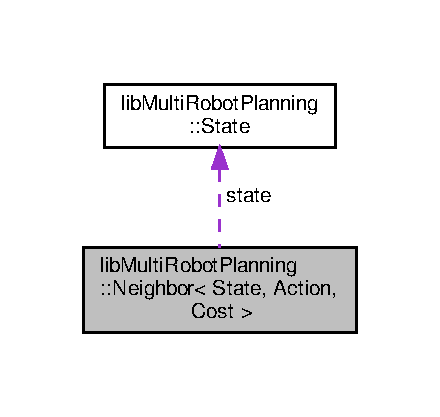
\includegraphics[width=211pt]{structlib_multi_robot_planning_1_1_neighbor__coll__graph}
\end{center}
\end{figure}
\subsection*{Public Member Functions}
\begin{DoxyCompactItemize}
\item 
\hyperlink{structlib_multi_robot_planning_1_1_neighbor_a048152420e26c75abca920a4c5060c42}{Neighbor} (const \hyperlink{structlib_multi_robot_planning_1_1_state}{State} \&\hyperlink{structlib_multi_robot_planning_1_1_neighbor_ad4930766ec86e82ae342ffe94f5e0da4}{state}, const \hyperlink{namespacelib_multi_robot_planning_aba73fb71693f86a324adfa0e41e1053d}{Action} \&\hyperlink{structlib_multi_robot_planning_1_1_neighbor_a8b50ab4edc18e97d809dcd89c42bed44}{action}, Cost \hyperlink{structlib_multi_robot_planning_1_1_neighbor_af269be36c1200896a5990f7ee3d9da27}{cost})
\end{DoxyCompactItemize}
\subsection*{Public Attributes}
\begin{DoxyCompactItemize}
\item 
\hyperlink{structlib_multi_robot_planning_1_1_state}{State} \hyperlink{structlib_multi_robot_planning_1_1_neighbor_ad4930766ec86e82ae342ffe94f5e0da4}{state}
\begin{DoxyCompactList}\small\item\em neighboring state \end{DoxyCompactList}\item 
\hyperlink{namespacelib_multi_robot_planning_aba73fb71693f86a324adfa0e41e1053d}{Action} \hyperlink{structlib_multi_robot_planning_1_1_neighbor_a8b50ab4edc18e97d809dcd89c42bed44}{action}
\begin{DoxyCompactList}\small\item\em action to get to the neighboring state \end{DoxyCompactList}\item 
Cost \hyperlink{structlib_multi_robot_planning_1_1_neighbor_af269be36c1200896a5990f7ee3d9da27}{cost}
\begin{DoxyCompactList}\small\item\em cost to get to the neighboring state \end{DoxyCompactList}\end{DoxyCompactItemize}


\subsection{Detailed Description}
\subsubsection*{template$<$typename State, typename Action, typename Cost$>$\newline
struct lib\+Multi\+Robot\+Planning\+::\+Neighbor$<$ State, Action, Cost $>$}

Represents state transations. 

This class represents a transition from a start state applying an action with the given cost.


\begin{DoxyTemplParams}{Template Parameters}
{\em \hyperlink{structlib_multi_robot_planning_1_1_state}{State}} & Custom state for the search. Needs to be copy\textquotesingle{}able \\
\hline
{\em Action} & Custom action for the search. Needs to be copy\textquotesingle{}able \\
\hline
{\em Cost} & Custom Cost type (integer or floating point types) \\
\hline
\end{DoxyTemplParams}


Definition at line 15 of file neighbor.\+hpp.



\subsection{Constructor \& Destructor Documentation}
\mbox{\Hypertarget{structlib_multi_robot_planning_1_1_neighbor_a048152420e26c75abca920a4c5060c42}\label{structlib_multi_robot_planning_1_1_neighbor_a048152420e26c75abca920a4c5060c42}} 
\index{lib\+Multi\+Robot\+Planning\+::\+Neighbor@{lib\+Multi\+Robot\+Planning\+::\+Neighbor}!Neighbor@{Neighbor}}
\index{Neighbor@{Neighbor}!lib\+Multi\+Robot\+Planning\+::\+Neighbor@{lib\+Multi\+Robot\+Planning\+::\+Neighbor}}
\subsubsection{\texorpdfstring{Neighbor()}{Neighbor()}}
{\footnotesize\ttfamily template$<$typename State, typename Action, typename Cost$>$ \\
\hyperlink{structlib_multi_robot_planning_1_1_neighbor}{lib\+Multi\+Robot\+Planning\+::\+Neighbor}$<$ \hyperlink{structlib_multi_robot_planning_1_1_state}{State}, \hyperlink{namespacelib_multi_robot_planning_aba73fb71693f86a324adfa0e41e1053d}{Action}, Cost $>$\+::\hyperlink{structlib_multi_robot_planning_1_1_neighbor}{Neighbor} (\begin{DoxyParamCaption}\item[{const \hyperlink{structlib_multi_robot_planning_1_1_state}{State} \&}]{state,  }\item[{const \hyperlink{namespacelib_multi_robot_planning_aba73fb71693f86a324adfa0e41e1053d}{Action} \&}]{action,  }\item[{Cost}]{cost }\end{DoxyParamCaption})\hspace{0.3cm}{\ttfamily [inline]}}



Definition at line 16 of file neighbor.\+hpp.



\subsection{Member Data Documentation}
\mbox{\Hypertarget{structlib_multi_robot_planning_1_1_neighbor_a8b50ab4edc18e97d809dcd89c42bed44}\label{structlib_multi_robot_planning_1_1_neighbor_a8b50ab4edc18e97d809dcd89c42bed44}} 
\index{lib\+Multi\+Robot\+Planning\+::\+Neighbor@{lib\+Multi\+Robot\+Planning\+::\+Neighbor}!action@{action}}
\index{action@{action}!lib\+Multi\+Robot\+Planning\+::\+Neighbor@{lib\+Multi\+Robot\+Planning\+::\+Neighbor}}
\subsubsection{\texorpdfstring{action}{action}}
{\footnotesize\ttfamily template$<$typename State, typename Action, typename Cost$>$ \\
\hyperlink{namespacelib_multi_robot_planning_aba73fb71693f86a324adfa0e41e1053d}{Action} \hyperlink{structlib_multi_robot_planning_1_1_neighbor}{lib\+Multi\+Robot\+Planning\+::\+Neighbor}$<$ \hyperlink{structlib_multi_robot_planning_1_1_state}{State}, \hyperlink{namespacelib_multi_robot_planning_aba73fb71693f86a324adfa0e41e1053d}{Action}, Cost $>$\+::action}



action to get to the neighboring state 



Definition at line 22 of file neighbor.\+hpp.

\mbox{\Hypertarget{structlib_multi_robot_planning_1_1_neighbor_af269be36c1200896a5990f7ee3d9da27}\label{structlib_multi_robot_planning_1_1_neighbor_af269be36c1200896a5990f7ee3d9da27}} 
\index{lib\+Multi\+Robot\+Planning\+::\+Neighbor@{lib\+Multi\+Robot\+Planning\+::\+Neighbor}!cost@{cost}}
\index{cost@{cost}!lib\+Multi\+Robot\+Planning\+::\+Neighbor@{lib\+Multi\+Robot\+Planning\+::\+Neighbor}}
\subsubsection{\texorpdfstring{cost}{cost}}
{\footnotesize\ttfamily template$<$typename State, typename Action, typename Cost$>$ \\
Cost \hyperlink{structlib_multi_robot_planning_1_1_neighbor}{lib\+Multi\+Robot\+Planning\+::\+Neighbor}$<$ \hyperlink{structlib_multi_robot_planning_1_1_state}{State}, \hyperlink{namespacelib_multi_robot_planning_aba73fb71693f86a324adfa0e41e1053d}{Action}, Cost $>$\+::cost}



cost to get to the neighboring state 



Definition at line 24 of file neighbor.\+hpp.

\mbox{\Hypertarget{structlib_multi_robot_planning_1_1_neighbor_ad4930766ec86e82ae342ffe94f5e0da4}\label{structlib_multi_robot_planning_1_1_neighbor_ad4930766ec86e82ae342ffe94f5e0da4}} 
\index{lib\+Multi\+Robot\+Planning\+::\+Neighbor@{lib\+Multi\+Robot\+Planning\+::\+Neighbor}!state@{state}}
\index{state@{state}!lib\+Multi\+Robot\+Planning\+::\+Neighbor@{lib\+Multi\+Robot\+Planning\+::\+Neighbor}}
\subsubsection{\texorpdfstring{state}{state}}
{\footnotesize\ttfamily template$<$typename State, typename Action, typename Cost$>$ \\
\hyperlink{structlib_multi_robot_planning_1_1_state}{State} \hyperlink{structlib_multi_robot_planning_1_1_neighbor}{lib\+Multi\+Robot\+Planning\+::\+Neighbor}$<$ \hyperlink{structlib_multi_robot_planning_1_1_state}{State}, \hyperlink{namespacelib_multi_robot_planning_aba73fb71693f86a324adfa0e41e1053d}{Action}, Cost $>$\+::state}



neighboring state 



Definition at line 20 of file neighbor.\+hpp.



The documentation for this struct was generated from the following file\+:\begin{DoxyCompactItemize}
\item 
third\+\_\+party/ecbs/include/\hyperlink{neighbor_8hpp}{neighbor.\+hpp}\end{DoxyCompactItemize}

\hypertarget{classlib_corridor_gen_1_1_param}{}\section{lib\+Corridor\+Gen\+:\+:Param Class Reference}
\label{classlib_corridor_gen_1_1_param}\index{lib\+Corridor\+Gen\+::\+Param@{lib\+Corridor\+Gen\+::\+Param}}


{\ttfamily \#include $<$param.\+hpp$>$}

\subsection*{Public Member Functions}
\begin{DoxyCompactItemize}
\item 
bool \hyperlink{classlib_corridor_gen_1_1_param_aafe3d5fb62dfc1c9f8fb700d7a1c9c8c}{init} (const ros\+::\+Node\+Handle \&nh)
\end{DoxyCompactItemize}
\subsection*{Public Attributes}
\begin{DoxyCompactItemize}
\item 
bool \hyperlink{classlib_corridor_gen_1_1_param_adc4669a46a8c18a89b60215bdeca3bcf}{log}
\item 
std\+::string \hyperlink{classlib_corridor_gen_1_1_param_af04ce9a5803f4aaaf506a78ffdbe0546}{package\+\_\+path}
\item 
double \hyperlink{classlib_corridor_gen_1_1_param_a9d17f9a691182310aeecbdebd975a269}{agent\+\_\+xy\+\_\+size}
\item 
double \hyperlink{classlib_corridor_gen_1_1_param_aaced15e8c6140c18534c6bbcfee7a691}{agent\+\_\+z\+\_\+size}
\item 
double \hyperlink{classlib_corridor_gen_1_1_param_ac66ab234f907a104db8885416fc10d59}{agent\+\_\+speed}
\item 
double \hyperlink{classlib_corridor_gen_1_1_param_aee380de2012d264db56877c2f5a7dcbe}{world\+\_\+x\+\_\+min}
\item 
double \hyperlink{classlib_corridor_gen_1_1_param_a0336ed1d72b56d608009c3f39ebb7161}{world\+\_\+y\+\_\+min}
\item 
double \hyperlink{classlib_corridor_gen_1_1_param_a02c38a168cd5ffa1f02d7c36789dd292}{world\+\_\+z\+\_\+min}
\item 
double \hyperlink{classlib_corridor_gen_1_1_param_add7ad22a3f830a9e90155e2dc489ff63}{world\+\_\+x\+\_\+max}
\item 
double \hyperlink{classlib_corridor_gen_1_1_param_a51c9e2bcfdf2d406499ced2e72e43c8a}{world\+\_\+y\+\_\+max}
\item 
double \hyperlink{classlib_corridor_gen_1_1_param_a37b098a4fc172dfb774c17e05586460e}{world\+\_\+z\+\_\+max}
\item 
double \hyperlink{classlib_corridor_gen_1_1_param_afd5159caa58faeffb2a3806738247d8b}{grid\+\_\+xy\+\_\+res}
\item 
double \hyperlink{classlib_corridor_gen_1_1_param_af829f93c4548e29f87827eee2028631c}{grid\+\_\+z\+\_\+res}
\item 
double \hyperlink{classlib_corridor_gen_1_1_param_acd5526e270bafe02c9b1d7aa45af46d8}{grid\+\_\+margin}
\item 
double \hyperlink{classlib_corridor_gen_1_1_param_a0493fd580cced6fa09382ee331dea7d1}{box\+\_\+xy\+\_\+res}
\item 
double \hyperlink{classlib_corridor_gen_1_1_param_a57326306f4c8312d30e3cf3345dbf6b3}{box\+\_\+z\+\_\+res}
\item 
double \hyperlink{classlib_corridor_gen_1_1_param_ac6dc24f51f8f0a382ad1d57f799dbfd1}{mission\+\_\+start\+\_\+x}
\item 
double \hyperlink{classlib_corridor_gen_1_1_param_a302faea25f3c79852939fac4231c7659}{mission\+\_\+start\+\_\+y}
\item 
double \hyperlink{classlib_corridor_gen_1_1_param_a4697fad18a536c8b1b1367d3497640d0}{mission\+\_\+goal\+\_\+x}
\item 
double \hyperlink{classlib_corridor_gen_1_1_param_a4691919af4489f2cf4047a4d569b644f}{mission\+\_\+goal\+\_\+y}
\item 
double \hyperlink{classlib_corridor_gen_1_1_param_a4cad71446f0b95b7ab94d9a3a484821c}{time\+\_\+step}
\item 
std\+::vector$<$ double $>$ \hyperlink{classlib_corridor_gen_1_1_param_a5619419eba931d2e33d49a52699a08d8}{color}
\end{DoxyCompactItemize}


\subsection{Detailed Description}


Definition at line 7 of file param.\+hpp.



\subsection{Member Function Documentation}
\mbox{\Hypertarget{classlib_corridor_gen_1_1_param_aafe3d5fb62dfc1c9f8fb700d7a1c9c8c}\label{classlib_corridor_gen_1_1_param_aafe3d5fb62dfc1c9f8fb700d7a1c9c8c}} 
\index{lib\+Corridor\+Gen\+::\+Param@{lib\+Corridor\+Gen\+::\+Param}!init@{init}}
\index{init@{init}!lib\+Corridor\+Gen\+::\+Param@{lib\+Corridor\+Gen\+::\+Param}}
\subsubsection{\texorpdfstring{init()}{init()}}
{\footnotesize\ttfamily bool lib\+Corridor\+Gen\+::\+Param\+::init (\begin{DoxyParamCaption}\item[{const ros\+::\+Node\+Handle \&}]{nh }\end{DoxyParamCaption})}



Definition at line 41 of file param.\+hpp.

Here is the caller graph for this function\+:
\nopagebreak
\begin{figure}[H]
\begin{center}
\leavevmode
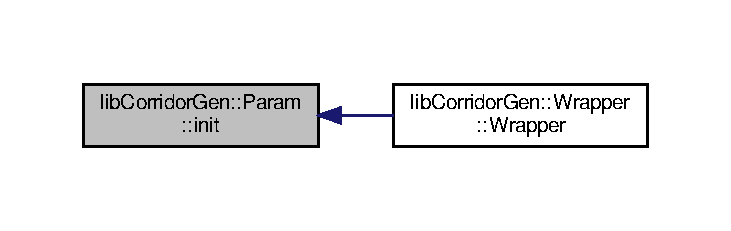
\includegraphics[width=350pt]{classlib_corridor_gen_1_1_param_aafe3d5fb62dfc1c9f8fb700d7a1c9c8c_icgraph}
\end{center}
\end{figure}


\subsection{Member Data Documentation}
\mbox{\Hypertarget{classlib_corridor_gen_1_1_param_ac66ab234f907a104db8885416fc10d59}\label{classlib_corridor_gen_1_1_param_ac66ab234f907a104db8885416fc10d59}} 
\index{lib\+Corridor\+Gen\+::\+Param@{lib\+Corridor\+Gen\+::\+Param}!agent\+\_\+speed@{agent\+\_\+speed}}
\index{agent\+\_\+speed@{agent\+\_\+speed}!lib\+Corridor\+Gen\+::\+Param@{lib\+Corridor\+Gen\+::\+Param}}
\subsubsection{\texorpdfstring{agent\+\_\+speed}{agent\_speed}}
{\footnotesize\ttfamily double lib\+Corridor\+Gen\+::\+Param\+::agent\+\_\+speed}



Definition at line 14 of file param.\+hpp.

\mbox{\Hypertarget{classlib_corridor_gen_1_1_param_a9d17f9a691182310aeecbdebd975a269}\label{classlib_corridor_gen_1_1_param_a9d17f9a691182310aeecbdebd975a269}} 
\index{lib\+Corridor\+Gen\+::\+Param@{lib\+Corridor\+Gen\+::\+Param}!agent\+\_\+xy\+\_\+size@{agent\+\_\+xy\+\_\+size}}
\index{agent\+\_\+xy\+\_\+size@{agent\+\_\+xy\+\_\+size}!lib\+Corridor\+Gen\+::\+Param@{lib\+Corridor\+Gen\+::\+Param}}
\subsubsection{\texorpdfstring{agent\+\_\+xy\+\_\+size}{agent\_xy\_size}}
{\footnotesize\ttfamily double lib\+Corridor\+Gen\+::\+Param\+::agent\+\_\+xy\+\_\+size}



Definition at line 12 of file param.\+hpp.

\mbox{\Hypertarget{classlib_corridor_gen_1_1_param_aaced15e8c6140c18534c6bbcfee7a691}\label{classlib_corridor_gen_1_1_param_aaced15e8c6140c18534c6bbcfee7a691}} 
\index{lib\+Corridor\+Gen\+::\+Param@{lib\+Corridor\+Gen\+::\+Param}!agent\+\_\+z\+\_\+size@{agent\+\_\+z\+\_\+size}}
\index{agent\+\_\+z\+\_\+size@{agent\+\_\+z\+\_\+size}!lib\+Corridor\+Gen\+::\+Param@{lib\+Corridor\+Gen\+::\+Param}}
\subsubsection{\texorpdfstring{agent\+\_\+z\+\_\+size}{agent\_z\_size}}
{\footnotesize\ttfamily double lib\+Corridor\+Gen\+::\+Param\+::agent\+\_\+z\+\_\+size}



Definition at line 13 of file param.\+hpp.

\mbox{\Hypertarget{classlib_corridor_gen_1_1_param_a0493fd580cced6fa09382ee331dea7d1}\label{classlib_corridor_gen_1_1_param_a0493fd580cced6fa09382ee331dea7d1}} 
\index{lib\+Corridor\+Gen\+::\+Param@{lib\+Corridor\+Gen\+::\+Param}!box\+\_\+xy\+\_\+res@{box\+\_\+xy\+\_\+res}}
\index{box\+\_\+xy\+\_\+res@{box\+\_\+xy\+\_\+res}!lib\+Corridor\+Gen\+::\+Param@{lib\+Corridor\+Gen\+::\+Param}}
\subsubsection{\texorpdfstring{box\+\_\+xy\+\_\+res}{box\_xy\_res}}
{\footnotesize\ttfamily double lib\+Corridor\+Gen\+::\+Param\+::box\+\_\+xy\+\_\+res}



Definition at line 27 of file param.\+hpp.

\mbox{\Hypertarget{classlib_corridor_gen_1_1_param_a57326306f4c8312d30e3cf3345dbf6b3}\label{classlib_corridor_gen_1_1_param_a57326306f4c8312d30e3cf3345dbf6b3}} 
\index{lib\+Corridor\+Gen\+::\+Param@{lib\+Corridor\+Gen\+::\+Param}!box\+\_\+z\+\_\+res@{box\+\_\+z\+\_\+res}}
\index{box\+\_\+z\+\_\+res@{box\+\_\+z\+\_\+res}!lib\+Corridor\+Gen\+::\+Param@{lib\+Corridor\+Gen\+::\+Param}}
\subsubsection{\texorpdfstring{box\+\_\+z\+\_\+res}{box\_z\_res}}
{\footnotesize\ttfamily double lib\+Corridor\+Gen\+::\+Param\+::box\+\_\+z\+\_\+res}



Definition at line 28 of file param.\+hpp.

\mbox{\Hypertarget{classlib_corridor_gen_1_1_param_a5619419eba931d2e33d49a52699a08d8}\label{classlib_corridor_gen_1_1_param_a5619419eba931d2e33d49a52699a08d8}} 
\index{lib\+Corridor\+Gen\+::\+Param@{lib\+Corridor\+Gen\+::\+Param}!color@{color}}
\index{color@{color}!lib\+Corridor\+Gen\+::\+Param@{lib\+Corridor\+Gen\+::\+Param}}
\subsubsection{\texorpdfstring{color}{color}}
{\footnotesize\ttfamily std\+::vector$<$double$>$ lib\+Corridor\+Gen\+::\+Param\+::color}



Definition at line 36 of file param.\+hpp.

\mbox{\Hypertarget{classlib_corridor_gen_1_1_param_acd5526e270bafe02c9b1d7aa45af46d8}\label{classlib_corridor_gen_1_1_param_acd5526e270bafe02c9b1d7aa45af46d8}} 
\index{lib\+Corridor\+Gen\+::\+Param@{lib\+Corridor\+Gen\+::\+Param}!grid\+\_\+margin@{grid\+\_\+margin}}
\index{grid\+\_\+margin@{grid\+\_\+margin}!lib\+Corridor\+Gen\+::\+Param@{lib\+Corridor\+Gen\+::\+Param}}
\subsubsection{\texorpdfstring{grid\+\_\+margin}{grid\_margin}}
{\footnotesize\ttfamily double lib\+Corridor\+Gen\+::\+Param\+::grid\+\_\+margin}



Definition at line 25 of file param.\+hpp.

\mbox{\Hypertarget{classlib_corridor_gen_1_1_param_afd5159caa58faeffb2a3806738247d8b}\label{classlib_corridor_gen_1_1_param_afd5159caa58faeffb2a3806738247d8b}} 
\index{lib\+Corridor\+Gen\+::\+Param@{lib\+Corridor\+Gen\+::\+Param}!grid\+\_\+xy\+\_\+res@{grid\+\_\+xy\+\_\+res}}
\index{grid\+\_\+xy\+\_\+res@{grid\+\_\+xy\+\_\+res}!lib\+Corridor\+Gen\+::\+Param@{lib\+Corridor\+Gen\+::\+Param}}
\subsubsection{\texorpdfstring{grid\+\_\+xy\+\_\+res}{grid\_xy\_res}}
{\footnotesize\ttfamily double lib\+Corridor\+Gen\+::\+Param\+::grid\+\_\+xy\+\_\+res}



Definition at line 23 of file param.\+hpp.

\mbox{\Hypertarget{classlib_corridor_gen_1_1_param_af829f93c4548e29f87827eee2028631c}\label{classlib_corridor_gen_1_1_param_af829f93c4548e29f87827eee2028631c}} 
\index{lib\+Corridor\+Gen\+::\+Param@{lib\+Corridor\+Gen\+::\+Param}!grid\+\_\+z\+\_\+res@{grid\+\_\+z\+\_\+res}}
\index{grid\+\_\+z\+\_\+res@{grid\+\_\+z\+\_\+res}!lib\+Corridor\+Gen\+::\+Param@{lib\+Corridor\+Gen\+::\+Param}}
\subsubsection{\texorpdfstring{grid\+\_\+z\+\_\+res}{grid\_z\_res}}
{\footnotesize\ttfamily double lib\+Corridor\+Gen\+::\+Param\+::grid\+\_\+z\+\_\+res}



Definition at line 24 of file param.\+hpp.

\mbox{\Hypertarget{classlib_corridor_gen_1_1_param_adc4669a46a8c18a89b60215bdeca3bcf}\label{classlib_corridor_gen_1_1_param_adc4669a46a8c18a89b60215bdeca3bcf}} 
\index{lib\+Corridor\+Gen\+::\+Param@{lib\+Corridor\+Gen\+::\+Param}!log@{log}}
\index{log@{log}!lib\+Corridor\+Gen\+::\+Param@{lib\+Corridor\+Gen\+::\+Param}}
\subsubsection{\texorpdfstring{log}{log}}
{\footnotesize\ttfamily bool lib\+Corridor\+Gen\+::\+Param\+::log}



Definition at line 9 of file param.\+hpp.

\mbox{\Hypertarget{classlib_corridor_gen_1_1_param_a4697fad18a536c8b1b1367d3497640d0}\label{classlib_corridor_gen_1_1_param_a4697fad18a536c8b1b1367d3497640d0}} 
\index{lib\+Corridor\+Gen\+::\+Param@{lib\+Corridor\+Gen\+::\+Param}!mission\+\_\+goal\+\_\+x@{mission\+\_\+goal\+\_\+x}}
\index{mission\+\_\+goal\+\_\+x@{mission\+\_\+goal\+\_\+x}!lib\+Corridor\+Gen\+::\+Param@{lib\+Corridor\+Gen\+::\+Param}}
\subsubsection{\texorpdfstring{mission\+\_\+goal\+\_\+x}{mission\_goal\_x}}
{\footnotesize\ttfamily double lib\+Corridor\+Gen\+::\+Param\+::mission\+\_\+goal\+\_\+x}



Definition at line 32 of file param.\+hpp.

\mbox{\Hypertarget{classlib_corridor_gen_1_1_param_a4691919af4489f2cf4047a4d569b644f}\label{classlib_corridor_gen_1_1_param_a4691919af4489f2cf4047a4d569b644f}} 
\index{lib\+Corridor\+Gen\+::\+Param@{lib\+Corridor\+Gen\+::\+Param}!mission\+\_\+goal\+\_\+y@{mission\+\_\+goal\+\_\+y}}
\index{mission\+\_\+goal\+\_\+y@{mission\+\_\+goal\+\_\+y}!lib\+Corridor\+Gen\+::\+Param@{lib\+Corridor\+Gen\+::\+Param}}
\subsubsection{\texorpdfstring{mission\+\_\+goal\+\_\+y}{mission\_goal\_y}}
{\footnotesize\ttfamily double lib\+Corridor\+Gen\+::\+Param\+::mission\+\_\+goal\+\_\+y}



Definition at line 33 of file param.\+hpp.

\mbox{\Hypertarget{classlib_corridor_gen_1_1_param_ac6dc24f51f8f0a382ad1d57f799dbfd1}\label{classlib_corridor_gen_1_1_param_ac6dc24f51f8f0a382ad1d57f799dbfd1}} 
\index{lib\+Corridor\+Gen\+::\+Param@{lib\+Corridor\+Gen\+::\+Param}!mission\+\_\+start\+\_\+x@{mission\+\_\+start\+\_\+x}}
\index{mission\+\_\+start\+\_\+x@{mission\+\_\+start\+\_\+x}!lib\+Corridor\+Gen\+::\+Param@{lib\+Corridor\+Gen\+::\+Param}}
\subsubsection{\texorpdfstring{mission\+\_\+start\+\_\+x}{mission\_start\_x}}
{\footnotesize\ttfamily double lib\+Corridor\+Gen\+::\+Param\+::mission\+\_\+start\+\_\+x}



Definition at line 30 of file param.\+hpp.

\mbox{\Hypertarget{classlib_corridor_gen_1_1_param_a302faea25f3c79852939fac4231c7659}\label{classlib_corridor_gen_1_1_param_a302faea25f3c79852939fac4231c7659}} 
\index{lib\+Corridor\+Gen\+::\+Param@{lib\+Corridor\+Gen\+::\+Param}!mission\+\_\+start\+\_\+y@{mission\+\_\+start\+\_\+y}}
\index{mission\+\_\+start\+\_\+y@{mission\+\_\+start\+\_\+y}!lib\+Corridor\+Gen\+::\+Param@{lib\+Corridor\+Gen\+::\+Param}}
\subsubsection{\texorpdfstring{mission\+\_\+start\+\_\+y}{mission\_start\_y}}
{\footnotesize\ttfamily double lib\+Corridor\+Gen\+::\+Param\+::mission\+\_\+start\+\_\+y}



Definition at line 31 of file param.\+hpp.

\mbox{\Hypertarget{classlib_corridor_gen_1_1_param_af04ce9a5803f4aaaf506a78ffdbe0546}\label{classlib_corridor_gen_1_1_param_af04ce9a5803f4aaaf506a78ffdbe0546}} 
\index{lib\+Corridor\+Gen\+::\+Param@{lib\+Corridor\+Gen\+::\+Param}!package\+\_\+path@{package\+\_\+path}}
\index{package\+\_\+path@{package\+\_\+path}!lib\+Corridor\+Gen\+::\+Param@{lib\+Corridor\+Gen\+::\+Param}}
\subsubsection{\texorpdfstring{package\+\_\+path}{package\_path}}
{\footnotesize\ttfamily std\+::string lib\+Corridor\+Gen\+::\+Param\+::package\+\_\+path}



Definition at line 10 of file param.\+hpp.

\mbox{\Hypertarget{classlib_corridor_gen_1_1_param_a4cad71446f0b95b7ab94d9a3a484821c}\label{classlib_corridor_gen_1_1_param_a4cad71446f0b95b7ab94d9a3a484821c}} 
\index{lib\+Corridor\+Gen\+::\+Param@{lib\+Corridor\+Gen\+::\+Param}!time\+\_\+step@{time\+\_\+step}}
\index{time\+\_\+step@{time\+\_\+step}!lib\+Corridor\+Gen\+::\+Param@{lib\+Corridor\+Gen\+::\+Param}}
\subsubsection{\texorpdfstring{time\+\_\+step}{time\_step}}
{\footnotesize\ttfamily double lib\+Corridor\+Gen\+::\+Param\+::time\+\_\+step}



Definition at line 35 of file param.\+hpp.

\mbox{\Hypertarget{classlib_corridor_gen_1_1_param_add7ad22a3f830a9e90155e2dc489ff63}\label{classlib_corridor_gen_1_1_param_add7ad22a3f830a9e90155e2dc489ff63}} 
\index{lib\+Corridor\+Gen\+::\+Param@{lib\+Corridor\+Gen\+::\+Param}!world\+\_\+x\+\_\+max@{world\+\_\+x\+\_\+max}}
\index{world\+\_\+x\+\_\+max@{world\+\_\+x\+\_\+max}!lib\+Corridor\+Gen\+::\+Param@{lib\+Corridor\+Gen\+::\+Param}}
\subsubsection{\texorpdfstring{world\+\_\+x\+\_\+max}{world\_x\_max}}
{\footnotesize\ttfamily double lib\+Corridor\+Gen\+::\+Param\+::world\+\_\+x\+\_\+max}



Definition at line 19 of file param.\+hpp.

\mbox{\Hypertarget{classlib_corridor_gen_1_1_param_aee380de2012d264db56877c2f5a7dcbe}\label{classlib_corridor_gen_1_1_param_aee380de2012d264db56877c2f5a7dcbe}} 
\index{lib\+Corridor\+Gen\+::\+Param@{lib\+Corridor\+Gen\+::\+Param}!world\+\_\+x\+\_\+min@{world\+\_\+x\+\_\+min}}
\index{world\+\_\+x\+\_\+min@{world\+\_\+x\+\_\+min}!lib\+Corridor\+Gen\+::\+Param@{lib\+Corridor\+Gen\+::\+Param}}
\subsubsection{\texorpdfstring{world\+\_\+x\+\_\+min}{world\_x\_min}}
{\footnotesize\ttfamily double lib\+Corridor\+Gen\+::\+Param\+::world\+\_\+x\+\_\+min}



Definition at line 16 of file param.\+hpp.

\mbox{\Hypertarget{classlib_corridor_gen_1_1_param_a51c9e2bcfdf2d406499ced2e72e43c8a}\label{classlib_corridor_gen_1_1_param_a51c9e2bcfdf2d406499ced2e72e43c8a}} 
\index{lib\+Corridor\+Gen\+::\+Param@{lib\+Corridor\+Gen\+::\+Param}!world\+\_\+y\+\_\+max@{world\+\_\+y\+\_\+max}}
\index{world\+\_\+y\+\_\+max@{world\+\_\+y\+\_\+max}!lib\+Corridor\+Gen\+::\+Param@{lib\+Corridor\+Gen\+::\+Param}}
\subsubsection{\texorpdfstring{world\+\_\+y\+\_\+max}{world\_y\_max}}
{\footnotesize\ttfamily double lib\+Corridor\+Gen\+::\+Param\+::world\+\_\+y\+\_\+max}



Definition at line 20 of file param.\+hpp.

\mbox{\Hypertarget{classlib_corridor_gen_1_1_param_a0336ed1d72b56d608009c3f39ebb7161}\label{classlib_corridor_gen_1_1_param_a0336ed1d72b56d608009c3f39ebb7161}} 
\index{lib\+Corridor\+Gen\+::\+Param@{lib\+Corridor\+Gen\+::\+Param}!world\+\_\+y\+\_\+min@{world\+\_\+y\+\_\+min}}
\index{world\+\_\+y\+\_\+min@{world\+\_\+y\+\_\+min}!lib\+Corridor\+Gen\+::\+Param@{lib\+Corridor\+Gen\+::\+Param}}
\subsubsection{\texorpdfstring{world\+\_\+y\+\_\+min}{world\_y\_min}}
{\footnotesize\ttfamily double lib\+Corridor\+Gen\+::\+Param\+::world\+\_\+y\+\_\+min}



Definition at line 17 of file param.\+hpp.

\mbox{\Hypertarget{classlib_corridor_gen_1_1_param_a37b098a4fc172dfb774c17e05586460e}\label{classlib_corridor_gen_1_1_param_a37b098a4fc172dfb774c17e05586460e}} 
\index{lib\+Corridor\+Gen\+::\+Param@{lib\+Corridor\+Gen\+::\+Param}!world\+\_\+z\+\_\+max@{world\+\_\+z\+\_\+max}}
\index{world\+\_\+z\+\_\+max@{world\+\_\+z\+\_\+max}!lib\+Corridor\+Gen\+::\+Param@{lib\+Corridor\+Gen\+::\+Param}}
\subsubsection{\texorpdfstring{world\+\_\+z\+\_\+max}{world\_z\_max}}
{\footnotesize\ttfamily double lib\+Corridor\+Gen\+::\+Param\+::world\+\_\+z\+\_\+max}



Definition at line 21 of file param.\+hpp.

\mbox{\Hypertarget{classlib_corridor_gen_1_1_param_a02c38a168cd5ffa1f02d7c36789dd292}\label{classlib_corridor_gen_1_1_param_a02c38a168cd5ffa1f02d7c36789dd292}} 
\index{lib\+Corridor\+Gen\+::\+Param@{lib\+Corridor\+Gen\+::\+Param}!world\+\_\+z\+\_\+min@{world\+\_\+z\+\_\+min}}
\index{world\+\_\+z\+\_\+min@{world\+\_\+z\+\_\+min}!lib\+Corridor\+Gen\+::\+Param@{lib\+Corridor\+Gen\+::\+Param}}
\subsubsection{\texorpdfstring{world\+\_\+z\+\_\+min}{world\_z\_min}}
{\footnotesize\ttfamily double lib\+Corridor\+Gen\+::\+Param\+::world\+\_\+z\+\_\+min}



Definition at line 18 of file param.\+hpp.



The documentation for this class was generated from the following file\+:\begin{DoxyCompactItemize}
\item 
include/\hyperlink{param_8hpp}{param.\+hpp}\end{DoxyCompactItemize}

\hypertarget{structlib_multi_robot_planning_1_1_plan_result}{}\section{lib\+Multi\+Robot\+Planning\+:\+:Plan\+Result$<$ State, Action, Cost $>$ Struct Template Reference}
\label{structlib_multi_robot_planning_1_1_plan_result}\index{lib\+Multi\+Robot\+Planning\+::\+Plan\+Result$<$ State, Action, Cost $>$@{lib\+Multi\+Robot\+Planning\+::\+Plan\+Result$<$ State, Action, Cost $>$}}


Represents the path for an agent.  




{\ttfamily \#include $<$planresult.\+hpp$>$}

\subsection*{Public Attributes}
\begin{DoxyCompactItemize}
\item 
std\+::vector$<$ std\+::pair$<$ \hyperlink{structlib_multi_robot_planning_1_1_state}{State}, Cost $>$ $>$ \hyperlink{structlib_multi_robot_planning_1_1_plan_result_ad1bd2882efca968d38165742bae0a511}{states}
\begin{DoxyCompactList}\small\item\em states and their g\+Score \end{DoxyCompactList}\item 
std\+::vector$<$ std\+::pair$<$ \hyperlink{namespacelib_multi_robot_planning_aba73fb71693f86a324adfa0e41e1053d}{Action}, Cost $>$ $>$ \hyperlink{structlib_multi_robot_planning_1_1_plan_result_aa868b92b5c742f6c662e69779fbd09a4}{actions}
\begin{DoxyCompactList}\small\item\em actions and their cost \end{DoxyCompactList}\item 
Cost \hyperlink{structlib_multi_robot_planning_1_1_plan_result_ab340aeae4fdabbd0345403e9fa609d9a}{cost}
\begin{DoxyCompactList}\small\item\em actual cost of the result \end{DoxyCompactList}\item 
Cost \hyperlink{structlib_multi_robot_planning_1_1_plan_result_aefdd2f68b906f207ded16bfe46e0f7b0}{fmin}
\begin{DoxyCompactList}\small\item\em lower bound of the cost (for suboptimal solvers) \end{DoxyCompactList}\end{DoxyCompactItemize}


\subsection{Detailed Description}
\subsubsection*{template$<$typename State, typename Action, typename Cost$>$\newline
struct lib\+Multi\+Robot\+Planning\+::\+Plan\+Result$<$ State, Action, Cost $>$}

Represents the path for an agent. 

This class is used to store the result of a planner for a single agent. It has both the ordered list of states that need to be traversed as well as the ordered list of actions together with their respective costs


\begin{DoxyTemplParams}{Template Parameters}
{\em \hyperlink{structlib_multi_robot_planning_1_1_state}{State}} & Custom state for the search. Needs to be copy\textquotesingle{}able \\
\hline
{\em Action} & Custom action for the search. Needs to be copy\textquotesingle{}able \\
\hline
{\em Cost} & Custom Cost type (integer or floating point types) \\
\hline
\end{DoxyTemplParams}


Definition at line 19 of file planresult.\+hpp.



\subsection{Member Data Documentation}
\mbox{\Hypertarget{structlib_multi_robot_planning_1_1_plan_result_aa868b92b5c742f6c662e69779fbd09a4}\label{structlib_multi_robot_planning_1_1_plan_result_aa868b92b5c742f6c662e69779fbd09a4}} 
\index{lib\+Multi\+Robot\+Planning\+::\+Plan\+Result@{lib\+Multi\+Robot\+Planning\+::\+Plan\+Result}!actions@{actions}}
\index{actions@{actions}!lib\+Multi\+Robot\+Planning\+::\+Plan\+Result@{lib\+Multi\+Robot\+Planning\+::\+Plan\+Result}}
\subsubsection{\texorpdfstring{actions}{actions}}
{\footnotesize\ttfamily template$<$typename State, typename Action, typename Cost$>$ \\
std\+::vector$<$std\+::pair$<$\hyperlink{namespacelib_multi_robot_planning_aba73fb71693f86a324adfa0e41e1053d}{Action}, Cost$>$ $>$ \hyperlink{structlib_multi_robot_planning_1_1_plan_result}{lib\+Multi\+Robot\+Planning\+::\+Plan\+Result}$<$ \hyperlink{structlib_multi_robot_planning_1_1_state}{State}, \hyperlink{namespacelib_multi_robot_planning_aba73fb71693f86a324adfa0e41e1053d}{Action}, Cost $>$\+::actions}



actions and their cost 



Definition at line 23 of file planresult.\+hpp.

\mbox{\Hypertarget{structlib_multi_robot_planning_1_1_plan_result_ab340aeae4fdabbd0345403e9fa609d9a}\label{structlib_multi_robot_planning_1_1_plan_result_ab340aeae4fdabbd0345403e9fa609d9a}} 
\index{lib\+Multi\+Robot\+Planning\+::\+Plan\+Result@{lib\+Multi\+Robot\+Planning\+::\+Plan\+Result}!cost@{cost}}
\index{cost@{cost}!lib\+Multi\+Robot\+Planning\+::\+Plan\+Result@{lib\+Multi\+Robot\+Planning\+::\+Plan\+Result}}
\subsubsection{\texorpdfstring{cost}{cost}}
{\footnotesize\ttfamily template$<$typename State, typename Action, typename Cost$>$ \\
Cost \hyperlink{structlib_multi_robot_planning_1_1_plan_result}{lib\+Multi\+Robot\+Planning\+::\+Plan\+Result}$<$ \hyperlink{structlib_multi_robot_planning_1_1_state}{State}, \hyperlink{namespacelib_multi_robot_planning_aba73fb71693f86a324adfa0e41e1053d}{Action}, Cost $>$\+::cost}



actual cost of the result 



Definition at line 25 of file planresult.\+hpp.

\mbox{\Hypertarget{structlib_multi_robot_planning_1_1_plan_result_aefdd2f68b906f207ded16bfe46e0f7b0}\label{structlib_multi_robot_planning_1_1_plan_result_aefdd2f68b906f207ded16bfe46e0f7b0}} 
\index{lib\+Multi\+Robot\+Planning\+::\+Plan\+Result@{lib\+Multi\+Robot\+Planning\+::\+Plan\+Result}!fmin@{fmin}}
\index{fmin@{fmin}!lib\+Multi\+Robot\+Planning\+::\+Plan\+Result@{lib\+Multi\+Robot\+Planning\+::\+Plan\+Result}}
\subsubsection{\texorpdfstring{fmin}{fmin}}
{\footnotesize\ttfamily template$<$typename State, typename Action, typename Cost$>$ \\
Cost \hyperlink{structlib_multi_robot_planning_1_1_plan_result}{lib\+Multi\+Robot\+Planning\+::\+Plan\+Result}$<$ \hyperlink{structlib_multi_robot_planning_1_1_state}{State}, \hyperlink{namespacelib_multi_robot_planning_aba73fb71693f86a324adfa0e41e1053d}{Action}, Cost $>$\+::fmin}



lower bound of the cost (for suboptimal solvers) 



Definition at line 27 of file planresult.\+hpp.

\mbox{\Hypertarget{structlib_multi_robot_planning_1_1_plan_result_ad1bd2882efca968d38165742bae0a511}\label{structlib_multi_robot_planning_1_1_plan_result_ad1bd2882efca968d38165742bae0a511}} 
\index{lib\+Multi\+Robot\+Planning\+::\+Plan\+Result@{lib\+Multi\+Robot\+Planning\+::\+Plan\+Result}!states@{states}}
\index{states@{states}!lib\+Multi\+Robot\+Planning\+::\+Plan\+Result@{lib\+Multi\+Robot\+Planning\+::\+Plan\+Result}}
\subsubsection{\texorpdfstring{states}{states}}
{\footnotesize\ttfamily template$<$typename State, typename Action, typename Cost$>$ \\
std\+::vector$<$std\+::pair$<$\hyperlink{structlib_multi_robot_planning_1_1_state}{State}, Cost$>$ $>$ \hyperlink{structlib_multi_robot_planning_1_1_plan_result}{lib\+Multi\+Robot\+Planning\+::\+Plan\+Result}$<$ \hyperlink{structlib_multi_robot_planning_1_1_state}{State}, \hyperlink{namespacelib_multi_robot_planning_aba73fb71693f86a324adfa0e41e1053d}{Action}, Cost $>$\+::states}



states and their g\+Score 



Definition at line 21 of file planresult.\+hpp.



The documentation for this struct was generated from the following file\+:\begin{DoxyCompactItemize}
\item 
third\+\_\+party/ecbs/include/\hyperlink{planresult_8hpp}{planresult.\+hpp}\end{DoxyCompactItemize}

\hypertarget{classlib_corridor_gen_1_1_result_publisher}{}\section{lib\+Corridor\+Gen\+:\+:Result\+Publisher Class Reference}
\label{classlib_corridor_gen_1_1_result_publisher}\index{lib\+Corridor\+Gen\+::\+Result\+Publisher@{lib\+Corridor\+Gen\+::\+Result\+Publisher}}


{\ttfamily \#include $<$result\+\_\+publisher.\+hpp$>$}

\subsection*{Public Member Functions}
\begin{DoxyCompactItemize}
\item 
\hyperlink{classlib_corridor_gen_1_1_result_publisher_a45476376dd8eb2a32c2357f7fb2e23b4}{Result\+Publisher} (const ros\+::\+Node\+Handle \&\+\_\+nh, std\+::shared\+\_\+ptr$<$ \hyperlink{classlib_corridor_gen_1_1_corridor}{Corridor} $>$ \+\_\+corridor\+\_\+obj, std\+::shared\+\_\+ptr$<$ \hyperlink{classlib_corridor_gen_1_1_init_traj_planner}{Init\+Traj\+Planner} $>$ \+\_\+init\+Traj\+Planner\+\_\+obj, \hyperlink{classlib_corridor_gen_1_1_param}{Param} \+\_\+param)
\item 
void \hyperlink{classlib_corridor_gen_1_1_result_publisher_ac44b00acc1fbb46fb1b0ba1473b32145}{update} (double current\+\_\+time)
\item 
void \hyperlink{classlib_corridor_gen_1_1_result_publisher_a846ddb44d304b996236505af060c760d}{publish} ()
\end{DoxyCompactItemize}


\subsection{Detailed Description}


Definition at line 23 of file result\+\_\+publisher.\+hpp.



\subsection{Constructor \& Destructor Documentation}
\mbox{\Hypertarget{classlib_corridor_gen_1_1_result_publisher_a45476376dd8eb2a32c2357f7fb2e23b4}\label{classlib_corridor_gen_1_1_result_publisher_a45476376dd8eb2a32c2357f7fb2e23b4}} 
\index{lib\+Corridor\+Gen\+::\+Result\+Publisher@{lib\+Corridor\+Gen\+::\+Result\+Publisher}!Result\+Publisher@{Result\+Publisher}}
\index{Result\+Publisher@{Result\+Publisher}!lib\+Corridor\+Gen\+::\+Result\+Publisher@{lib\+Corridor\+Gen\+::\+Result\+Publisher}}
\subsubsection{\texorpdfstring{Result\+Publisher()}{ResultPublisher()}}
{\footnotesize\ttfamily lib\+Corridor\+Gen\+::\+Result\+Publisher\+::\+Result\+Publisher (\begin{DoxyParamCaption}\item[{const ros\+::\+Node\+Handle \&}]{\+\_\+nh,  }\item[{std\+::shared\+\_\+ptr$<$ \hyperlink{classlib_corridor_gen_1_1_corridor}{Corridor} $>$}]{\+\_\+corridor\+\_\+obj,  }\item[{std\+::shared\+\_\+ptr$<$ \hyperlink{classlib_corridor_gen_1_1_init_traj_planner}{Init\+Traj\+Planner} $>$}]{\+\_\+init\+Traj\+Planner\+\_\+obj,  }\item[{\hyperlink{classlib_corridor_gen_1_1_param}{Param}}]{\+\_\+param }\end{DoxyParamCaption})\hspace{0.3cm}{\ttfamily [inline]}}



Definition at line 25 of file result\+\_\+publisher.\+hpp.



\subsection{Member Function Documentation}
\mbox{\Hypertarget{classlib_corridor_gen_1_1_result_publisher_a846ddb44d304b996236505af060c760d}\label{classlib_corridor_gen_1_1_result_publisher_a846ddb44d304b996236505af060c760d}} 
\index{lib\+Corridor\+Gen\+::\+Result\+Publisher@{lib\+Corridor\+Gen\+::\+Result\+Publisher}!publish@{publish}}
\index{publish@{publish}!lib\+Corridor\+Gen\+::\+Result\+Publisher@{lib\+Corridor\+Gen\+::\+Result\+Publisher}}
\subsubsection{\texorpdfstring{publish()}{publish()}}
{\footnotesize\ttfamily void lib\+Corridor\+Gen\+::\+Result\+Publisher\+::publish (\begin{DoxyParamCaption}{ }\end{DoxyParamCaption})\hspace{0.3cm}{\ttfamily [inline]}}



Definition at line 45 of file result\+\_\+publisher.\+hpp.

\mbox{\Hypertarget{classlib_corridor_gen_1_1_result_publisher_ac44b00acc1fbb46fb1b0ba1473b32145}\label{classlib_corridor_gen_1_1_result_publisher_ac44b00acc1fbb46fb1b0ba1473b32145}} 
\index{lib\+Corridor\+Gen\+::\+Result\+Publisher@{lib\+Corridor\+Gen\+::\+Result\+Publisher}!update@{update}}
\index{update@{update}!lib\+Corridor\+Gen\+::\+Result\+Publisher@{lib\+Corridor\+Gen\+::\+Result\+Publisher}}
\subsubsection{\texorpdfstring{update()}{update()}}
{\footnotesize\ttfamily void lib\+Corridor\+Gen\+::\+Result\+Publisher\+::update (\begin{DoxyParamCaption}\item[{double}]{current\+\_\+time }\end{DoxyParamCaption})\hspace{0.3cm}{\ttfamily [inline]}}



Definition at line 39 of file result\+\_\+publisher.\+hpp.



The documentation for this class was generated from the following file\+:\begin{DoxyCompactItemize}
\item 
include/\hyperlink{result__publisher_8hpp}{result\+\_\+publisher.\+hpp}\end{DoxyCompactItemize}

\hypertarget{class_scoped_timer}{}\section{Scoped\+Timer Class Reference}
\label{class_scoped_timer}\index{Scoped\+Timer@{Scoped\+Timer}}


{\ttfamily \#include $<$timer.\+hpp$>$}



Inheritance diagram for Scoped\+Timer\+:
\nopagebreak
\begin{figure}[H]
\begin{center}
\leavevmode
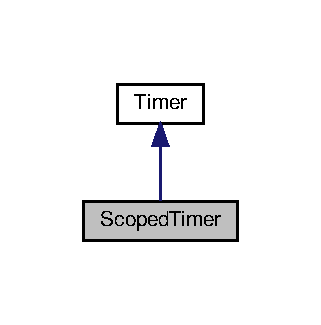
\includegraphics[width=154pt]{class_scoped_timer__inherit__graph}
\end{center}
\end{figure}


Collaboration diagram for Scoped\+Timer\+:
\nopagebreak
\begin{figure}[H]
\begin{center}
\leavevmode
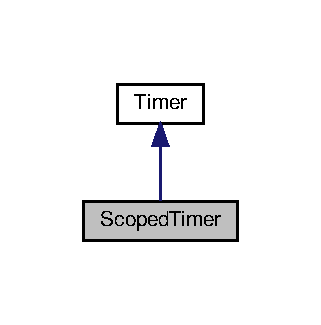
\includegraphics[width=154pt]{class_scoped_timer__coll__graph}
\end{center}
\end{figure}
\subsection*{Public Member Functions}
\begin{DoxyCompactItemize}
\item 
\hyperlink{class_scoped_timer_a7bc7d8cca2444b07382d565b321d1f82}{Scoped\+Timer} ()
\item 
\hyperlink{class_scoped_timer_a338ced0c8c39fe3d3e89e1b09d29f589}{$\sim$\+Scoped\+Timer} ()
\end{DoxyCompactItemize}


\subsection{Detailed Description}


Definition at line 27 of file timer.\+hpp.



\subsection{Constructor \& Destructor Documentation}
\mbox{\Hypertarget{class_scoped_timer_a7bc7d8cca2444b07382d565b321d1f82}\label{class_scoped_timer_a7bc7d8cca2444b07382d565b321d1f82}} 
\index{Scoped\+Timer@{Scoped\+Timer}!Scoped\+Timer@{Scoped\+Timer}}
\index{Scoped\+Timer@{Scoped\+Timer}!Scoped\+Timer@{Scoped\+Timer}}
\subsubsection{\texorpdfstring{Scoped\+Timer()}{ScopedTimer()}}
{\footnotesize\ttfamily Scoped\+Timer\+::\+Scoped\+Timer (\begin{DoxyParamCaption}{ }\end{DoxyParamCaption})\hspace{0.3cm}{\ttfamily [inline]}}



Definition at line 29 of file timer.\+hpp.

\mbox{\Hypertarget{class_scoped_timer_a338ced0c8c39fe3d3e89e1b09d29f589}\label{class_scoped_timer_a338ced0c8c39fe3d3e89e1b09d29f589}} 
\index{Scoped\+Timer@{Scoped\+Timer}!````~Scoped\+Timer@{$\sim$\+Scoped\+Timer}}
\index{````~Scoped\+Timer@{$\sim$\+Scoped\+Timer}!Scoped\+Timer@{Scoped\+Timer}}
\subsubsection{\texorpdfstring{$\sim$\+Scoped\+Timer()}{~ScopedTimer()}}
{\footnotesize\ttfamily Scoped\+Timer\+::$\sim$\+Scoped\+Timer (\begin{DoxyParamCaption}{ }\end{DoxyParamCaption})\hspace{0.3cm}{\ttfamily [inline]}}



Definition at line 31 of file timer.\+hpp.

Here is the call graph for this function\+:
\nopagebreak
\begin{figure}[H]
\begin{center}
\leavevmode
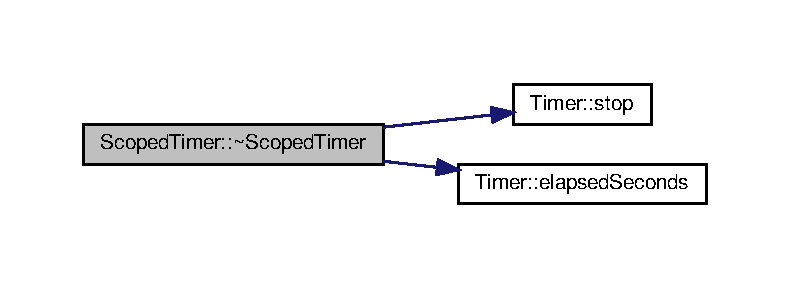
\includegraphics[width=350pt]{class_scoped_timer_a338ced0c8c39fe3d3e89e1b09d29f589_cgraph}
\end{center}
\end{figure}


The documentation for this class was generated from the following file\+:\begin{DoxyCompactItemize}
\item 
include/\hyperlink{timer_8hpp}{timer.\+hpp}\end{DoxyCompactItemize}

\hypertarget{struct_state}{}\section{State Struct Reference}
\label{struct_state}\index{State@{State}}
\subsection*{Public Member Functions}
\begin{DoxyCompactItemize}
\item 
\hyperlink{struct_state_a200e450f63a590ee3a777b60684963ee}{State} (int \hyperlink{struct_state_aafa13753373691d8ea3327717c61ef32}{x}, int \hyperlink{struct_state_a5dcf4a949618c21b85eb39ad41dfb08e}{y})
\item 
\hyperlink{struct_state_ad463f272453461a57c8b9e11f6cad8b6}{State} (const \hyperlink{struct_state}{State} \&)=default
\item 
\hyperlink{struct_state_a28668e1b15e6d6cfb63106769db218bc}{State} (\hyperlink{struct_state}{State} \&\&)=default
\item 
\hyperlink{struct_state}{State} \& \hyperlink{struct_state_a0c83d166ff2b6603a8e11c58d867e76f}{operator=} (const \hyperlink{struct_state}{State} \&)=default
\item 
\hyperlink{struct_state}{State} \& \hyperlink{struct_state_aa8d6ba634492b0c922f7dac1b87873c3}{operator=} (\hyperlink{struct_state}{State} \&\&)=default
\item 
bool \hyperlink{struct_state_ab98d310aaceb21737346521c5bc6fc6c}{operator==} (const \hyperlink{struct_state}{State} \&other) const
\item 
\hyperlink{struct_state_a044f9afae99d62ad92d1c10932e9be92}{State} (int \hyperlink{struct_state_aafa13753373691d8ea3327717c61ef32}{x}, int \hyperlink{struct_state_a5dcf4a949618c21b85eb39ad41dfb08e}{y}, int \hyperlink{struct_state_afbfffdf9a289cde788f99498adf1a0e5}{z})
\item 
\hyperlink{struct_state_ad463f272453461a57c8b9e11f6cad8b6}{State} (const \hyperlink{struct_state}{State} \&)=default
\item 
\hyperlink{struct_state_a28668e1b15e6d6cfb63106769db218bc}{State} (\hyperlink{struct_state}{State} \&\&)=default
\item 
\hyperlink{struct_state}{State} \& \hyperlink{struct_state_a0c83d166ff2b6603a8e11c58d867e76f}{operator=} (const \hyperlink{struct_state}{State} \&)=default
\item 
\hyperlink{struct_state}{State} \& \hyperlink{struct_state_aa8d6ba634492b0c922f7dac1b87873c3}{operator=} (\hyperlink{struct_state}{State} \&\&)=default
\item 
bool \hyperlink{struct_state_ab98d310aaceb21737346521c5bc6fc6c}{operator==} (const \hyperlink{struct_state}{State} \&other) const
\item 
\hyperlink{struct_state_acd7182e04da1e5c712fdda9a0dd329bd}{State} (int \hyperlink{struct_state_a66c39d91e41d0f477758d00af0300a8a}{time}, int \hyperlink{struct_state_aafa13753373691d8ea3327717c61ef32}{x}, int \hyperlink{struct_state_a5dcf4a949618c21b85eb39ad41dfb08e}{y}, int \hyperlink{struct_state_afbfffdf9a289cde788f99498adf1a0e5}{z})
\item 
bool \hyperlink{struct_state_ad7c923d78b138998c9f9f9674fbdd93a}{operator==} (const \hyperlink{struct_state}{State} \&s) const
\item 
bool \hyperlink{struct_state_a6d429325c836ad81fd1d95eec0051663}{equal\+Except\+Time} (const \hyperlink{struct_state}{State} \&s) const
\item 
\hyperlink{struct_state_acd7182e04da1e5c712fdda9a0dd329bd}{State} (int \hyperlink{struct_state_a66c39d91e41d0f477758d00af0300a8a}{time}, int \hyperlink{struct_state_aafa13753373691d8ea3327717c61ef32}{x}, int \hyperlink{struct_state_a5dcf4a949618c21b85eb39ad41dfb08e}{y}, int \hyperlink{struct_state_afbfffdf9a289cde788f99498adf1a0e5}{z})
\item 
bool \hyperlink{struct_state_ad7c923d78b138998c9f9f9674fbdd93a}{operator==} (const \hyperlink{struct_state}{State} \&s) const
\item 
bool \hyperlink{struct_state_a6d429325c836ad81fd1d95eec0051663}{equal\+Except\+Time} (const \hyperlink{struct_state}{State} \&s) const
\end{DoxyCompactItemize}
\subsection*{Public Attributes}
\begin{DoxyCompactItemize}
\item 
int \hyperlink{struct_state_aafa13753373691d8ea3327717c61ef32}{x}
\item 
int \hyperlink{struct_state_a5dcf4a949618c21b85eb39ad41dfb08e}{y}
\item 
int \hyperlink{struct_state_afbfffdf9a289cde788f99498adf1a0e5}{z}
\item 
int \hyperlink{struct_state_a66c39d91e41d0f477758d00af0300a8a}{time}
\end{DoxyCompactItemize}
\subsection*{Friends}
\begin{DoxyCompactItemize}
\item 
std\+::ostream \& \hyperlink{struct_state_a5604754e63c801276d20313c05a68847}{operator$<$$<$} (std\+::ostream \&os, const \hyperlink{struct_state}{State} \&s)
\item 
std\+::ostream \& \hyperlink{struct_state_a5604754e63c801276d20313c05a68847}{operator$<$$<$} (std\+::ostream \&os, const \hyperlink{struct_state}{State} \&s)
\item 
std\+::ostream \& \hyperlink{struct_state_a5604754e63c801276d20313c05a68847}{operator$<$$<$} (std\+::ostream \&os, const \hyperlink{struct_state}{State} \&s)
\item 
std\+::ostream \& \hyperlink{struct_state_a5604754e63c801276d20313c05a68847}{operator$<$$<$} (std\+::ostream \&os, const \hyperlink{struct_state}{State} \&s)
\end{DoxyCompactItemize}


\subsection{Detailed Description}


Definition at line 13 of file a\+\_\+star.\+cpp.



\subsection{Constructor \& Destructor Documentation}
\mbox{\Hypertarget{struct_state_a200e450f63a590ee3a777b60684963ee}\label{struct_state_a200e450f63a590ee3a777b60684963ee}} 
\index{State@{State}!State@{State}}
\index{State@{State}!State@{State}}
\subsubsection{\texorpdfstring{State()}{State()}\hspace{0.1cm}{\footnotesize\ttfamily [1/8]}}
{\footnotesize\ttfamily State\+::\+State (\begin{DoxyParamCaption}\item[{int}]{x,  }\item[{int}]{y }\end{DoxyParamCaption})\hspace{0.3cm}{\ttfamily [inline]}}



Definition at line 14 of file a\+\_\+star.\+cpp.

Here is the call graph for this function\+:
\nopagebreak
\begin{figure}[H]
\begin{center}
\leavevmode
\includegraphics[width=272pt]{struct_state_a200e450f63a590ee3a777b60684963ee_cgraph}
\end{center}
\end{figure}
Here is the caller graph for this function\+:
\nopagebreak
\begin{figure}[H]
\begin{center}
\leavevmode
\includegraphics[width=254pt]{struct_state_a200e450f63a590ee3a777b60684963ee_icgraph}
\end{center}
\end{figure}
\mbox{\Hypertarget{struct_state_ad463f272453461a57c8b9e11f6cad8b6}\label{struct_state_ad463f272453461a57c8b9e11f6cad8b6}} 
\index{State@{State}!State@{State}}
\index{State@{State}!State@{State}}
\subsubsection{\texorpdfstring{State()}{State()}\hspace{0.1cm}{\footnotesize\ttfamily [2/8]}}
{\footnotesize\ttfamily State\+::\+State (\begin{DoxyParamCaption}\item[{const \hyperlink{struct_state}{State} \&}]{ }\end{DoxyParamCaption})\hspace{0.3cm}{\ttfamily [default]}}

\mbox{\Hypertarget{struct_state_a28668e1b15e6d6cfb63106769db218bc}\label{struct_state_a28668e1b15e6d6cfb63106769db218bc}} 
\index{State@{State}!State@{State}}
\index{State@{State}!State@{State}}
\subsubsection{\texorpdfstring{State()}{State()}\hspace{0.1cm}{\footnotesize\ttfamily [3/8]}}
{\footnotesize\ttfamily State\+::\+State (\begin{DoxyParamCaption}\item[{\hyperlink{struct_state}{State} \&\&}]{ }\end{DoxyParamCaption})\hspace{0.3cm}{\ttfamily [default]}}

\mbox{\Hypertarget{struct_state_a044f9afae99d62ad92d1c10932e9be92}\label{struct_state_a044f9afae99d62ad92d1c10932e9be92}} 
\index{State@{State}!State@{State}}
\index{State@{State}!State@{State}}
\subsubsection{\texorpdfstring{State()}{State()}\hspace{0.1cm}{\footnotesize\ttfamily [4/8]}}
{\footnotesize\ttfamily State\+::\+State (\begin{DoxyParamCaption}\item[{int}]{x,  }\item[{int}]{y,  }\item[{int}]{z }\end{DoxyParamCaption})\hspace{0.3cm}{\ttfamily [inline]}}



Definition at line 14 of file a\+\_\+star\+\_\+epsilon.\+cpp.

Here is the call graph for this function\+:
\nopagebreak
\begin{figure}[H]
\begin{center}
\leavevmode
\includegraphics[width=350pt]{struct_state_a044f9afae99d62ad92d1c10932e9be92_cgraph}
\end{center}
\end{figure}
\mbox{\Hypertarget{struct_state_ad463f272453461a57c8b9e11f6cad8b6}\label{struct_state_ad463f272453461a57c8b9e11f6cad8b6}} 
\index{State@{State}!State@{State}}
\index{State@{State}!State@{State}}
\subsubsection{\texorpdfstring{State()}{State()}\hspace{0.1cm}{\footnotesize\ttfamily [5/8]}}
{\footnotesize\ttfamily State\+::\+State (\begin{DoxyParamCaption}\item[{const \hyperlink{struct_state}{State} \&}]{ }\end{DoxyParamCaption})\hspace{0.3cm}{\ttfamily [default]}}

\mbox{\Hypertarget{struct_state_a28668e1b15e6d6cfb63106769db218bc}\label{struct_state_a28668e1b15e6d6cfb63106769db218bc}} 
\index{State@{State}!State@{State}}
\index{State@{State}!State@{State}}
\subsubsection{\texorpdfstring{State()}{State()}\hspace{0.1cm}{\footnotesize\ttfamily [6/8]}}
{\footnotesize\ttfamily State\+::\+State (\begin{DoxyParamCaption}\item[{\hyperlink{struct_state}{State} \&\&}]{ }\end{DoxyParamCaption})\hspace{0.3cm}{\ttfamily [default]}}

\mbox{\Hypertarget{struct_state_acd7182e04da1e5c712fdda9a0dd329bd}\label{struct_state_acd7182e04da1e5c712fdda9a0dd329bd}} 
\index{State@{State}!State@{State}}
\index{State@{State}!State@{State}}
\subsubsection{\texorpdfstring{State()}{State()}\hspace{0.1cm}{\footnotesize\ttfamily [7/8]}}
{\footnotesize\ttfamily State\+::\+State (\begin{DoxyParamCaption}\item[{int}]{time,  }\item[{int}]{x,  }\item[{int}]{y,  }\item[{int}]{z }\end{DoxyParamCaption})\hspace{0.3cm}{\ttfamily [inline]}}



Definition at line 17 of file cbs.\+cpp.

\mbox{\Hypertarget{struct_state_acd7182e04da1e5c712fdda9a0dd329bd}\label{struct_state_acd7182e04da1e5c712fdda9a0dd329bd}} 
\index{State@{State}!State@{State}}
\index{State@{State}!State@{State}}
\subsubsection{\texorpdfstring{State()}{State()}\hspace{0.1cm}{\footnotesize\ttfamily [8/8]}}
{\footnotesize\ttfamily State\+::\+State (\begin{DoxyParamCaption}\item[{int}]{time,  }\item[{int}]{x,  }\item[{int}]{y,  }\item[{int}]{z }\end{DoxyParamCaption})\hspace{0.3cm}{\ttfamily [inline]}}



Definition at line 17 of file ecbs.\+cpp.



\subsection{Member Function Documentation}
\mbox{\Hypertarget{struct_state_a6d429325c836ad81fd1d95eec0051663}\label{struct_state_a6d429325c836ad81fd1d95eec0051663}} 
\index{State@{State}!equal\+Except\+Time@{equal\+Except\+Time}}
\index{equal\+Except\+Time@{equal\+Except\+Time}!State@{State}}
\subsubsection{\texorpdfstring{equal\+Except\+Time()}{equalExceptTime()}\hspace{0.1cm}{\footnotesize\ttfamily [1/2]}}
{\footnotesize\ttfamily bool State\+::equal\+Except\+Time (\begin{DoxyParamCaption}\item[{const \hyperlink{struct_state}{State} \&}]{s }\end{DoxyParamCaption}) const\hspace{0.3cm}{\ttfamily [inline]}}



Definition at line 23 of file cbs.\+cpp.

Here is the caller graph for this function\+:
\nopagebreak
\begin{figure}[H]
\begin{center}
\leavevmode
\includegraphics[width=350pt]{struct_state_a6d429325c836ad81fd1d95eec0051663_icgraph}
\end{center}
\end{figure}
\mbox{\Hypertarget{struct_state_a6d429325c836ad81fd1d95eec0051663}\label{struct_state_a6d429325c836ad81fd1d95eec0051663}} 
\index{State@{State}!equal\+Except\+Time@{equal\+Except\+Time}}
\index{equal\+Except\+Time@{equal\+Except\+Time}!State@{State}}
\subsubsection{\texorpdfstring{equal\+Except\+Time()}{equalExceptTime()}\hspace{0.1cm}{\footnotesize\ttfamily [2/2]}}
{\footnotesize\ttfamily bool State\+::equal\+Except\+Time (\begin{DoxyParamCaption}\item[{const \hyperlink{struct_state}{State} \&}]{s }\end{DoxyParamCaption}) const\hspace{0.3cm}{\ttfamily [inline]}}



Definition at line 23 of file ecbs.\+cpp.

\mbox{\Hypertarget{struct_state_a0c83d166ff2b6603a8e11c58d867e76f}\label{struct_state_a0c83d166ff2b6603a8e11c58d867e76f}} 
\index{State@{State}!operator=@{operator=}}
\index{operator=@{operator=}!State@{State}}
\subsubsection{\texorpdfstring{operator=()}{operator=()}\hspace{0.1cm}{\footnotesize\ttfamily [1/4]}}
{\footnotesize\ttfamily \hyperlink{struct_state}{State}\& State\+::operator= (\begin{DoxyParamCaption}\item[{const \hyperlink{struct_state}{State} \&}]{ }\end{DoxyParamCaption})\hspace{0.3cm}{\ttfamily [default]}}

\mbox{\Hypertarget{struct_state_a0c83d166ff2b6603a8e11c58d867e76f}\label{struct_state_a0c83d166ff2b6603a8e11c58d867e76f}} 
\index{State@{State}!operator=@{operator=}}
\index{operator=@{operator=}!State@{State}}
\subsubsection{\texorpdfstring{operator=()}{operator=()}\hspace{0.1cm}{\footnotesize\ttfamily [2/4]}}
{\footnotesize\ttfamily \hyperlink{struct_state}{State}\& State\+::operator= (\begin{DoxyParamCaption}\item[{const \hyperlink{struct_state}{State} \&}]{ }\end{DoxyParamCaption})\hspace{0.3cm}{\ttfamily [default]}}

Here is the caller graph for this function\+:
\nopagebreak
\begin{figure}[H]
\begin{center}
\leavevmode
\includegraphics[width=350pt]{struct_state_a0c83d166ff2b6603a8e11c58d867e76f_icgraph}
\end{center}
\end{figure}
\mbox{\Hypertarget{struct_state_aa8d6ba634492b0c922f7dac1b87873c3}\label{struct_state_aa8d6ba634492b0c922f7dac1b87873c3}} 
\index{State@{State}!operator=@{operator=}}
\index{operator=@{operator=}!State@{State}}
\subsubsection{\texorpdfstring{operator=()}{operator=()}\hspace{0.1cm}{\footnotesize\ttfamily [3/4]}}
{\footnotesize\ttfamily \hyperlink{struct_state}{State}\& State\+::operator= (\begin{DoxyParamCaption}\item[{\hyperlink{struct_state}{State} \&\&}]{ }\end{DoxyParamCaption})\hspace{0.3cm}{\ttfamily [default]}}

\mbox{\Hypertarget{struct_state_aa8d6ba634492b0c922f7dac1b87873c3}\label{struct_state_aa8d6ba634492b0c922f7dac1b87873c3}} 
\index{State@{State}!operator=@{operator=}}
\index{operator=@{operator=}!State@{State}}
\subsubsection{\texorpdfstring{operator=()}{operator=()}\hspace{0.1cm}{\footnotesize\ttfamily [4/4]}}
{\footnotesize\ttfamily \hyperlink{struct_state}{State}\& State\+::operator= (\begin{DoxyParamCaption}\item[{\hyperlink{struct_state}{State} \&\&}]{ }\end{DoxyParamCaption})\hspace{0.3cm}{\ttfamily [default]}}

\mbox{\Hypertarget{struct_state_ad7c923d78b138998c9f9f9674fbdd93a}\label{struct_state_ad7c923d78b138998c9f9f9674fbdd93a}} 
\index{State@{State}!operator==@{operator==}}
\index{operator==@{operator==}!State@{State}}
\subsubsection{\texorpdfstring{operator==()}{operator==()}\hspace{0.1cm}{\footnotesize\ttfamily [1/4]}}
{\footnotesize\ttfamily bool State\+::operator== (\begin{DoxyParamCaption}\item[{const \hyperlink{struct_state}{State} \&}]{s }\end{DoxyParamCaption}) const\hspace{0.3cm}{\ttfamily [inline]}}



Definition at line 19 of file ecbs.\+cpp.

\mbox{\Hypertarget{struct_state_ad7c923d78b138998c9f9f9674fbdd93a}\label{struct_state_ad7c923d78b138998c9f9f9674fbdd93a}} 
\index{State@{State}!operator==@{operator==}}
\index{operator==@{operator==}!State@{State}}
\subsubsection{\texorpdfstring{operator==()}{operator==()}\hspace{0.1cm}{\footnotesize\ttfamily [2/4]}}
{\footnotesize\ttfamily bool State\+::operator== (\begin{DoxyParamCaption}\item[{const \hyperlink{struct_state}{State} \&}]{s }\end{DoxyParamCaption}) const\hspace{0.3cm}{\ttfamily [inline]}}



Definition at line 19 of file cbs.\+cpp.

\mbox{\Hypertarget{struct_state_ab98d310aaceb21737346521c5bc6fc6c}\label{struct_state_ab98d310aaceb21737346521c5bc6fc6c}} 
\index{State@{State}!operator==@{operator==}}
\index{operator==@{operator==}!State@{State}}
\subsubsection{\texorpdfstring{operator==()}{operator==()}\hspace{0.1cm}{\footnotesize\ttfamily [3/4]}}
{\footnotesize\ttfamily bool State\+::operator== (\begin{DoxyParamCaption}\item[{const \hyperlink{struct_state}{State} \&}]{other }\end{DoxyParamCaption}) const\hspace{0.3cm}{\ttfamily [inline]}}



Definition at line 21 of file a\+\_\+star.\+cpp.

\mbox{\Hypertarget{struct_state_ab98d310aaceb21737346521c5bc6fc6c}\label{struct_state_ab98d310aaceb21737346521c5bc6fc6c}} 
\index{State@{State}!operator==@{operator==}}
\index{operator==@{operator==}!State@{State}}
\subsubsection{\texorpdfstring{operator==()}{operator==()}\hspace{0.1cm}{\footnotesize\ttfamily [4/4]}}
{\footnotesize\ttfamily bool State\+::operator== (\begin{DoxyParamCaption}\item[{const \hyperlink{struct_state}{State} \&}]{other }\end{DoxyParamCaption}) const\hspace{0.3cm}{\ttfamily [inline]}}



Definition at line 21 of file a\+\_\+star\+\_\+epsilon.\+cpp.



\subsection{Friends And Related Function Documentation}
\mbox{\Hypertarget{struct_state_a5604754e63c801276d20313c05a68847}\label{struct_state_a5604754e63c801276d20313c05a68847}} 
\index{State@{State}!operator$<$$<$@{operator$<$$<$}}
\index{operator$<$$<$@{operator$<$$<$}!State@{State}}
\subsubsection{\texorpdfstring{operator$<$$<$}{operator<<}\hspace{0.1cm}{\footnotesize\ttfamily [1/4]}}
{\footnotesize\ttfamily std\+::ostream\& operator$<$$<$ (\begin{DoxyParamCaption}\item[{std\+::ostream \&}]{os,  }\item[{const \hyperlink{struct_state}{State} \&}]{s }\end{DoxyParamCaption})\hspace{0.3cm}{\ttfamily [friend]}}



Definition at line 25 of file a\+\_\+star.\+cpp.

\mbox{\Hypertarget{struct_state_a5604754e63c801276d20313c05a68847}\label{struct_state_a5604754e63c801276d20313c05a68847}} 
\index{State@{State}!operator$<$$<$@{operator$<$$<$}}
\index{operator$<$$<$@{operator$<$$<$}!State@{State}}
\subsubsection{\texorpdfstring{operator$<$$<$}{operator<<}\hspace{0.1cm}{\footnotesize\ttfamily [2/4]}}
{\footnotesize\ttfamily std\+::ostream\& operator$<$$<$ (\begin{DoxyParamCaption}\item[{std\+::ostream \&}]{os,  }\item[{const \hyperlink{struct_state}{State} \&}]{s }\end{DoxyParamCaption})\hspace{0.3cm}{\ttfamily [friend]}}



Definition at line 25 of file ecbs.\+cpp.

\mbox{\Hypertarget{struct_state_a5604754e63c801276d20313c05a68847}\label{struct_state_a5604754e63c801276d20313c05a68847}} 
\index{State@{State}!operator$<$$<$@{operator$<$$<$}}
\index{operator$<$$<$@{operator$<$$<$}!State@{State}}
\subsubsection{\texorpdfstring{operator$<$$<$}{operator<<}\hspace{0.1cm}{\footnotesize\ttfamily [3/4]}}
{\footnotesize\ttfamily std\+::ostream\& operator$<$$<$ (\begin{DoxyParamCaption}\item[{std\+::ostream \&}]{os,  }\item[{const \hyperlink{struct_state}{State} \&}]{s }\end{DoxyParamCaption})\hspace{0.3cm}{\ttfamily [friend]}}



Definition at line 25 of file cbs.\+cpp.

\mbox{\Hypertarget{struct_state_a5604754e63c801276d20313c05a68847}\label{struct_state_a5604754e63c801276d20313c05a68847}} 
\index{State@{State}!operator$<$$<$@{operator$<$$<$}}
\index{operator$<$$<$@{operator$<$$<$}!State@{State}}
\subsubsection{\texorpdfstring{operator$<$$<$}{operator<<}\hspace{0.1cm}{\footnotesize\ttfamily [4/4]}}
{\footnotesize\ttfamily std\+::ostream\& operator$<$$<$ (\begin{DoxyParamCaption}\item[{std\+::ostream \&}]{os,  }\item[{const \hyperlink{struct_state}{State} \&}]{s }\end{DoxyParamCaption})\hspace{0.3cm}{\ttfamily [friend]}}



Definition at line 25 of file a\+\_\+star\+\_\+epsilon.\+cpp.



\subsection{Member Data Documentation}
\mbox{\Hypertarget{struct_state_a66c39d91e41d0f477758d00af0300a8a}\label{struct_state_a66c39d91e41d0f477758d00af0300a8a}} 
\index{State@{State}!time@{time}}
\index{time@{time}!State@{State}}
\subsubsection{\texorpdfstring{time}{time}}
{\footnotesize\ttfamily int State\+::time}



Definition at line 30 of file cbs.\+cpp.

\mbox{\Hypertarget{struct_state_aafa13753373691d8ea3327717c61ef32}\label{struct_state_aafa13753373691d8ea3327717c61ef32}} 
\index{State@{State}!x@{x}}
\index{x@{x}!State@{State}}
\subsubsection{\texorpdfstring{x}{x}}
{\footnotesize\ttfamily int State\+::x}



Definition at line 29 of file a\+\_\+star.\+cpp.

\mbox{\Hypertarget{struct_state_a5dcf4a949618c21b85eb39ad41dfb08e}\label{struct_state_a5dcf4a949618c21b85eb39ad41dfb08e}} 
\index{State@{State}!y@{y}}
\index{y@{y}!State@{State}}
\subsubsection{\texorpdfstring{y}{y}}
{\footnotesize\ttfamily int State\+::y}



Definition at line 30 of file a\+\_\+star.\+cpp.

\mbox{\Hypertarget{struct_state_afbfffdf9a289cde788f99498adf1a0e5}\label{struct_state_afbfffdf9a289cde788f99498adf1a0e5}} 
\index{State@{State}!z@{z}}
\index{z@{z}!State@{State}}
\subsubsection{\texorpdfstring{z}{z}}
{\footnotesize\ttfamily int State\+::z}



Definition at line 31 of file a\+\_\+star\+\_\+epsilon.\+cpp.



The documentation for this struct was generated from the following files\+:\begin{DoxyCompactItemize}
\item 
third\+\_\+party/ecbs/src/\hyperlink{a__star_8cpp}{a\+\_\+star.\+cpp}\item 
third\+\_\+party/ecbs/src/\hyperlink{a__star__epsilon_8cpp}{a\+\_\+star\+\_\+epsilon.\+cpp}\item 
third\+\_\+party/ecbs/src/\hyperlink{cbs_8cpp}{cbs.\+cpp}\item 
third\+\_\+party/ecbs/src/\hyperlink{ecbs_8cpp}{ecbs.\+cpp}\end{DoxyCompactItemize}

\hypertarget{structlib_multi_robot_planning_1_1_state}{}\section{lib\+Multi\+Robot\+Planning\+:\+:State Struct Reference}
\label{structlib_multi_robot_planning_1_1_state}\index{lib\+Multi\+Robot\+Planning\+::\+State@{lib\+Multi\+Robot\+Planning\+::\+State}}


{\ttfamily \#include $<$environment.\+hpp$>$}

\subsection*{Public Member Functions}
\begin{DoxyCompactItemize}
\item 
\hyperlink{structlib_multi_robot_planning_1_1_state_af7aabb0901e59446d9067f2747a85fc2}{State} (int \hyperlink{structlib_multi_robot_planning_1_1_state_aa17a0558cc7338969be67626bd17082a}{time}, int \hyperlink{structlib_multi_robot_planning_1_1_state_a33c79339cb6a22c402518cfb4414959f}{x}, int \hyperlink{structlib_multi_robot_planning_1_1_state_ad23e634dc9b9dbd7c1021c67aa0cce9c}{y}, int \hyperlink{structlib_multi_robot_planning_1_1_state_af73c034e22c1f2e6851a12c4c51c9199}{z})
\item 
bool \hyperlink{structlib_multi_robot_planning_1_1_state_ac4e1772061abe4e9e5eda48d0ffb3133}{operator==} (const \hyperlink{structlib_multi_robot_planning_1_1_state}{State} \&s) const
\item 
bool \hyperlink{structlib_multi_robot_planning_1_1_state_a1067b5c669fb82dce96b4f07476ea655}{equal\+Except\+Time} (const \hyperlink{structlib_multi_robot_planning_1_1_state}{State} \&s) const
\end{DoxyCompactItemize}
\subsection*{Public Attributes}
\begin{DoxyCompactItemize}
\item 
int \hyperlink{structlib_multi_robot_planning_1_1_state_aa17a0558cc7338969be67626bd17082a}{time}
\item 
int \hyperlink{structlib_multi_robot_planning_1_1_state_a33c79339cb6a22c402518cfb4414959f}{x}
\item 
int \hyperlink{structlib_multi_robot_planning_1_1_state_ad23e634dc9b9dbd7c1021c67aa0cce9c}{y}
\item 
int \hyperlink{structlib_multi_robot_planning_1_1_state_af73c034e22c1f2e6851a12c4c51c9199}{z}
\end{DoxyCompactItemize}
\subsection*{Friends}
\begin{DoxyCompactItemize}
\item 
std\+::ostream \& \hyperlink{structlib_multi_robot_planning_1_1_state_a5604754e63c801276d20313c05a68847}{operator$<$$<$} (std\+::ostream \&os, const \hyperlink{structlib_multi_robot_planning_1_1_state}{State} \&s)
\end{DoxyCompactItemize}


\subsection{Detailed Description}


Definition at line 17 of file environment.\+hpp.



\subsection{Constructor \& Destructor Documentation}
\mbox{\Hypertarget{structlib_multi_robot_planning_1_1_state_af7aabb0901e59446d9067f2747a85fc2}\label{structlib_multi_robot_planning_1_1_state_af7aabb0901e59446d9067f2747a85fc2}} 
\index{lib\+Multi\+Robot\+Planning\+::\+State@{lib\+Multi\+Robot\+Planning\+::\+State}!State@{State}}
\index{State@{State}!lib\+Multi\+Robot\+Planning\+::\+State@{lib\+Multi\+Robot\+Planning\+::\+State}}
\subsubsection{\texorpdfstring{State()}{State()}}
{\footnotesize\ttfamily lib\+Multi\+Robot\+Planning\+::\+State\+::\+State (\begin{DoxyParamCaption}\item[{int}]{time,  }\item[{int}]{x,  }\item[{int}]{y,  }\item[{int}]{z }\end{DoxyParamCaption})\hspace{0.3cm}{\ttfamily [inline]}}



Definition at line 18 of file environment.\+hpp.



\subsection{Member Function Documentation}
\mbox{\Hypertarget{structlib_multi_robot_planning_1_1_state_a1067b5c669fb82dce96b4f07476ea655}\label{structlib_multi_robot_planning_1_1_state_a1067b5c669fb82dce96b4f07476ea655}} 
\index{lib\+Multi\+Robot\+Planning\+::\+State@{lib\+Multi\+Robot\+Planning\+::\+State}!equal\+Except\+Time@{equal\+Except\+Time}}
\index{equal\+Except\+Time@{equal\+Except\+Time}!lib\+Multi\+Robot\+Planning\+::\+State@{lib\+Multi\+Robot\+Planning\+::\+State}}
\subsubsection{\texorpdfstring{equal\+Except\+Time()}{equalExceptTime()}}
{\footnotesize\ttfamily bool lib\+Multi\+Robot\+Planning\+::\+State\+::equal\+Except\+Time (\begin{DoxyParamCaption}\item[{const \hyperlink{structlib_multi_robot_planning_1_1_state}{State} \&}]{s }\end{DoxyParamCaption}) const\hspace{0.3cm}{\ttfamily [inline]}}



Definition at line 24 of file environment.\+hpp.

Here is the caller graph for this function\+:
\nopagebreak
\begin{figure}[H]
\begin{center}
\leavevmode
\includegraphics[width=350pt]{structlib_multi_robot_planning_1_1_state_a1067b5c669fb82dce96b4f07476ea655_icgraph}
\end{center}
\end{figure}
\mbox{\Hypertarget{structlib_multi_robot_planning_1_1_state_ac4e1772061abe4e9e5eda48d0ffb3133}\label{structlib_multi_robot_planning_1_1_state_ac4e1772061abe4e9e5eda48d0ffb3133}} 
\index{lib\+Multi\+Robot\+Planning\+::\+State@{lib\+Multi\+Robot\+Planning\+::\+State}!operator==@{operator==}}
\index{operator==@{operator==}!lib\+Multi\+Robot\+Planning\+::\+State@{lib\+Multi\+Robot\+Planning\+::\+State}}
\subsubsection{\texorpdfstring{operator==()}{operator==()}}
{\footnotesize\ttfamily bool lib\+Multi\+Robot\+Planning\+::\+State\+::operator== (\begin{DoxyParamCaption}\item[{const \hyperlink{structlib_multi_robot_planning_1_1_state}{State} \&}]{s }\end{DoxyParamCaption}) const\hspace{0.3cm}{\ttfamily [inline]}}



Definition at line 20 of file environment.\+hpp.



\subsection{Friends And Related Function Documentation}
\mbox{\Hypertarget{structlib_multi_robot_planning_1_1_state_a5604754e63c801276d20313c05a68847}\label{structlib_multi_robot_planning_1_1_state_a5604754e63c801276d20313c05a68847}} 
\index{lib\+Multi\+Robot\+Planning\+::\+State@{lib\+Multi\+Robot\+Planning\+::\+State}!operator$<$$<$@{operator$<$$<$}}
\index{operator$<$$<$@{operator$<$$<$}!lib\+Multi\+Robot\+Planning\+::\+State@{lib\+Multi\+Robot\+Planning\+::\+State}}
\subsubsection{\texorpdfstring{operator$<$$<$}{operator<<}}
{\footnotesize\ttfamily std\+::ostream\& operator$<$$<$ (\begin{DoxyParamCaption}\item[{std\+::ostream \&}]{os,  }\item[{const \hyperlink{structlib_multi_robot_planning_1_1_state}{State} \&}]{s }\end{DoxyParamCaption})\hspace{0.3cm}{\ttfamily [friend]}}



Definition at line 26 of file environment.\+hpp.



\subsection{Member Data Documentation}
\mbox{\Hypertarget{structlib_multi_robot_planning_1_1_state_aa17a0558cc7338969be67626bd17082a}\label{structlib_multi_robot_planning_1_1_state_aa17a0558cc7338969be67626bd17082a}} 
\index{lib\+Multi\+Robot\+Planning\+::\+State@{lib\+Multi\+Robot\+Planning\+::\+State}!time@{time}}
\index{time@{time}!lib\+Multi\+Robot\+Planning\+::\+State@{lib\+Multi\+Robot\+Planning\+::\+State}}
\subsubsection{\texorpdfstring{time}{time}}
{\footnotesize\ttfamily int lib\+Multi\+Robot\+Planning\+::\+State\+::time}



Definition at line 31 of file environment.\+hpp.

\mbox{\Hypertarget{structlib_multi_robot_planning_1_1_state_a33c79339cb6a22c402518cfb4414959f}\label{structlib_multi_robot_planning_1_1_state_a33c79339cb6a22c402518cfb4414959f}} 
\index{lib\+Multi\+Robot\+Planning\+::\+State@{lib\+Multi\+Robot\+Planning\+::\+State}!x@{x}}
\index{x@{x}!lib\+Multi\+Robot\+Planning\+::\+State@{lib\+Multi\+Robot\+Planning\+::\+State}}
\subsubsection{\texorpdfstring{x}{x}}
{\footnotesize\ttfamily int lib\+Multi\+Robot\+Planning\+::\+State\+::x}



Definition at line 32 of file environment.\+hpp.

\mbox{\Hypertarget{structlib_multi_robot_planning_1_1_state_ad23e634dc9b9dbd7c1021c67aa0cce9c}\label{structlib_multi_robot_planning_1_1_state_ad23e634dc9b9dbd7c1021c67aa0cce9c}} 
\index{lib\+Multi\+Robot\+Planning\+::\+State@{lib\+Multi\+Robot\+Planning\+::\+State}!y@{y}}
\index{y@{y}!lib\+Multi\+Robot\+Planning\+::\+State@{lib\+Multi\+Robot\+Planning\+::\+State}}
\subsubsection{\texorpdfstring{y}{y}}
{\footnotesize\ttfamily int lib\+Multi\+Robot\+Planning\+::\+State\+::y}



Definition at line 33 of file environment.\+hpp.

\mbox{\Hypertarget{structlib_multi_robot_planning_1_1_state_af73c034e22c1f2e6851a12c4c51c9199}\label{structlib_multi_robot_planning_1_1_state_af73c034e22c1f2e6851a12c4c51c9199}} 
\index{lib\+Multi\+Robot\+Planning\+::\+State@{lib\+Multi\+Robot\+Planning\+::\+State}!z@{z}}
\index{z@{z}!lib\+Multi\+Robot\+Planning\+::\+State@{lib\+Multi\+Robot\+Planning\+::\+State}}
\subsubsection{\texorpdfstring{z}{z}}
{\footnotesize\ttfamily int lib\+Multi\+Robot\+Planning\+::\+State\+::z}



Definition at line 34 of file environment.\+hpp.



The documentation for this struct was generated from the following file\+:\begin{DoxyCompactItemize}
\item 
third\+\_\+party/ecbs/include/\hyperlink{environment_8hpp}{environment.\+hpp}\end{DoxyCompactItemize}

\hypertarget{class_timer}{}\section{Timer Class Reference}
\label{class_timer}\index{Timer@{Timer}}


{\ttfamily \#include $<$timer.\+hpp$>$}



Inheritance diagram for Timer\+:
\nopagebreak
\begin{figure}[H]
\begin{center}
\leavevmode
\includegraphics[width=154pt]{class_timer__inherit__graph}
\end{center}
\end{figure}
\subsection*{Public Member Functions}
\begin{DoxyCompactItemize}
\item 
\hyperlink{class_timer_a5f16e8da27d2a5a5242dead46de05d97}{Timer} ()
\item 
void \hyperlink{class_timer_a9020542d73357a4eef512eefaf57524b}{reset} ()
\item 
void \hyperlink{class_timer_a63f0eb44b27402196590a03781515dba}{stop} ()
\item 
double \hyperlink{class_timer_ab98eee549aa6c69eb83de41ed555d1e0}{elapsed\+Seconds} () const
\end{DoxyCompactItemize}


\subsection{Detailed Description}


Definition at line 6 of file timer.\+hpp.



\subsection{Constructor \& Destructor Documentation}
\mbox{\Hypertarget{class_timer_a5f16e8da27d2a5a5242dead46de05d97}\label{class_timer_a5f16e8da27d2a5a5242dead46de05d97}} 
\index{Timer@{Timer}!Timer@{Timer}}
\index{Timer@{Timer}!Timer@{Timer}}
\subsubsection{\texorpdfstring{Timer()}{Timer()}}
{\footnotesize\ttfamily Timer\+::\+Timer (\begin{DoxyParamCaption}{ }\end{DoxyParamCaption})\hspace{0.3cm}{\ttfamily [inline]}}



Definition at line 8 of file timer.\+hpp.



\subsection{Member Function Documentation}
\mbox{\Hypertarget{class_timer_ab98eee549aa6c69eb83de41ed555d1e0}\label{class_timer_ab98eee549aa6c69eb83de41ed555d1e0}} 
\index{Timer@{Timer}!elapsed\+Seconds@{elapsed\+Seconds}}
\index{elapsed\+Seconds@{elapsed\+Seconds}!Timer@{Timer}}
\subsubsection{\texorpdfstring{elapsed\+Seconds()}{elapsedSeconds()}}
{\footnotesize\ttfamily double Timer\+::elapsed\+Seconds (\begin{DoxyParamCaption}{ }\end{DoxyParamCaption}) const\hspace{0.3cm}{\ttfamily [inline]}}



Definition at line 16 of file timer.\+hpp.

Here is the caller graph for this function\+:
\nopagebreak
\begin{figure}[H]
\begin{center}
\leavevmode
\includegraphics[width=350pt]{class_timer_ab98eee549aa6c69eb83de41ed555d1e0_icgraph}
\end{center}
\end{figure}
\mbox{\Hypertarget{class_timer_a9020542d73357a4eef512eefaf57524b}\label{class_timer_a9020542d73357a4eef512eefaf57524b}} 
\index{Timer@{Timer}!reset@{reset}}
\index{reset@{reset}!Timer@{Timer}}
\subsubsection{\texorpdfstring{reset()}{reset()}}
{\footnotesize\ttfamily void Timer\+::reset (\begin{DoxyParamCaption}{ }\end{DoxyParamCaption})\hspace{0.3cm}{\ttfamily [inline]}}



Definition at line 12 of file timer.\+hpp.

Here is the caller graph for this function\+:
\nopagebreak
\begin{figure}[H]
\begin{center}
\leavevmode
\includegraphics[width=350pt]{class_timer_a9020542d73357a4eef512eefaf57524b_icgraph}
\end{center}
\end{figure}
\mbox{\Hypertarget{class_timer_a63f0eb44b27402196590a03781515dba}\label{class_timer_a63f0eb44b27402196590a03781515dba}} 
\index{Timer@{Timer}!stop@{stop}}
\index{stop@{stop}!Timer@{Timer}}
\subsubsection{\texorpdfstring{stop()}{stop()}}
{\footnotesize\ttfamily void Timer\+::stop (\begin{DoxyParamCaption}{ }\end{DoxyParamCaption})\hspace{0.3cm}{\ttfamily [inline]}}



Definition at line 14 of file timer.\+hpp.

Here is the caller graph for this function\+:
\nopagebreak
\begin{figure}[H]
\begin{center}
\leavevmode
\includegraphics[width=350pt]{class_timer_a63f0eb44b27402196590a03781515dba_icgraph}
\end{center}
\end{figure}


The documentation for this class was generated from the following file\+:\begin{DoxyCompactItemize}
\item 
include/\hyperlink{timer_8hpp}{timer.\+hpp}\end{DoxyCompactItemize}

\hypertarget{struct_vertex_constraint}{}\section{Vertex\+Constraint Struct Reference}
\label{struct_vertex_constraint}\index{Vertex\+Constraint@{Vertex\+Constraint}}
\subsection*{Public Member Functions}
\begin{DoxyCompactItemize}
\item 
\hyperlink{struct_vertex_constraint_a9916de476d15970c6be19739d89b8ff3}{Vertex\+Constraint} (int \hyperlink{struct_vertex_constraint_a524c257a521498f549e35a966c5dc900}{time}, int \hyperlink{struct_vertex_constraint_a23167b86e213a24d74bb8a15472b862a}{x}, int \hyperlink{struct_vertex_constraint_a1c20e6282ccaeb862046c483c72ebd98}{y}, int \hyperlink{struct_vertex_constraint_a57867ee08f9c72a86684ea759693011f}{z})
\item 
bool \hyperlink{struct_vertex_constraint_a7c3dc8c528e5047776be956697979552}{operator$<$} (const \hyperlink{struct_vertex_constraint}{Vertex\+Constraint} \&other) const
\item 
bool \hyperlink{struct_vertex_constraint_aa1479e4f7de0f75536f144d224661f4b}{operator==} (const \hyperlink{struct_vertex_constraint}{Vertex\+Constraint} \&other) const
\item 
\hyperlink{struct_vertex_constraint_a9916de476d15970c6be19739d89b8ff3}{Vertex\+Constraint} (int \hyperlink{struct_vertex_constraint_a524c257a521498f549e35a966c5dc900}{time}, int \hyperlink{struct_vertex_constraint_a23167b86e213a24d74bb8a15472b862a}{x}, int \hyperlink{struct_vertex_constraint_a1c20e6282ccaeb862046c483c72ebd98}{y}, int \hyperlink{struct_vertex_constraint_a57867ee08f9c72a86684ea759693011f}{z})
\item 
bool \hyperlink{struct_vertex_constraint_a7c3dc8c528e5047776be956697979552}{operator$<$} (const \hyperlink{struct_vertex_constraint}{Vertex\+Constraint} \&other) const
\item 
bool \hyperlink{struct_vertex_constraint_aa1479e4f7de0f75536f144d224661f4b}{operator==} (const \hyperlink{struct_vertex_constraint}{Vertex\+Constraint} \&other) const
\end{DoxyCompactItemize}
\subsection*{Public Attributes}
\begin{DoxyCompactItemize}
\item 
int \hyperlink{struct_vertex_constraint_a524c257a521498f549e35a966c5dc900}{time}
\item 
int \hyperlink{struct_vertex_constraint_a23167b86e213a24d74bb8a15472b862a}{x}
\item 
int \hyperlink{struct_vertex_constraint_a1c20e6282ccaeb862046c483c72ebd98}{y}
\item 
int \hyperlink{struct_vertex_constraint_a57867ee08f9c72a86684ea759693011f}{z}
\end{DoxyCompactItemize}
\subsection*{Friends}
\begin{DoxyCompactItemize}
\item 
std\+::ostream \& \hyperlink{struct_vertex_constraint_a673f5d8fdc4898875720dddfd6c80e68}{operator$<$$<$} (std\+::ostream \&os, const \hyperlink{struct_vertex_constraint}{Vertex\+Constraint} \&c)
\item 
std\+::ostream \& \hyperlink{struct_vertex_constraint_a673f5d8fdc4898875720dddfd6c80e68}{operator$<$$<$} (std\+::ostream \&os, const \hyperlink{struct_vertex_constraint}{Vertex\+Constraint} \&c)
\end{DoxyCompactItemize}


\subsection{Detailed Description}


Definition at line 120 of file cbs.\+cpp.



\subsection{Constructor \& Destructor Documentation}
\mbox{\Hypertarget{struct_vertex_constraint_a9916de476d15970c6be19739d89b8ff3}\label{struct_vertex_constraint_a9916de476d15970c6be19739d89b8ff3}} 
\index{Vertex\+Constraint@{Vertex\+Constraint}!Vertex\+Constraint@{Vertex\+Constraint}}
\index{Vertex\+Constraint@{Vertex\+Constraint}!Vertex\+Constraint@{Vertex\+Constraint}}
\subsubsection{\texorpdfstring{Vertex\+Constraint()}{VertexConstraint()}\hspace{0.1cm}{\footnotesize\ttfamily [1/2]}}
{\footnotesize\ttfamily Vertex\+Constraint\+::\+Vertex\+Constraint (\begin{DoxyParamCaption}\item[{int}]{time,  }\item[{int}]{x,  }\item[{int}]{y,  }\item[{int}]{z }\end{DoxyParamCaption})\hspace{0.3cm}{\ttfamily [inline]}}



Definition at line 121 of file cbs.\+cpp.

\mbox{\Hypertarget{struct_vertex_constraint_a9916de476d15970c6be19739d89b8ff3}\label{struct_vertex_constraint_a9916de476d15970c6be19739d89b8ff3}} 
\index{Vertex\+Constraint@{Vertex\+Constraint}!Vertex\+Constraint@{Vertex\+Constraint}}
\index{Vertex\+Constraint@{Vertex\+Constraint}!Vertex\+Constraint@{Vertex\+Constraint}}
\subsubsection{\texorpdfstring{Vertex\+Constraint()}{VertexConstraint()}\hspace{0.1cm}{\footnotesize\ttfamily [2/2]}}
{\footnotesize\ttfamily Vertex\+Constraint\+::\+Vertex\+Constraint (\begin{DoxyParamCaption}\item[{int}]{time,  }\item[{int}]{x,  }\item[{int}]{y,  }\item[{int}]{z }\end{DoxyParamCaption})\hspace{0.3cm}{\ttfamily [inline]}}



Definition at line 121 of file ecbs.\+cpp.



\subsection{Member Function Documentation}
\mbox{\Hypertarget{struct_vertex_constraint_a7c3dc8c528e5047776be956697979552}\label{struct_vertex_constraint_a7c3dc8c528e5047776be956697979552}} 
\index{Vertex\+Constraint@{Vertex\+Constraint}!operator$<$@{operator$<$}}
\index{operator$<$@{operator$<$}!Vertex\+Constraint@{Vertex\+Constraint}}
\subsubsection{\texorpdfstring{operator$<$()}{operator<()}\hspace{0.1cm}{\footnotesize\ttfamily [1/2]}}
{\footnotesize\ttfamily bool Vertex\+Constraint\+::operator$<$ (\begin{DoxyParamCaption}\item[{const \hyperlink{struct_vertex_constraint}{Vertex\+Constraint} \&}]{other }\end{DoxyParamCaption}) const\hspace{0.3cm}{\ttfamily [inline]}}



Definition at line 127 of file cbs.\+cpp.

\mbox{\Hypertarget{struct_vertex_constraint_a7c3dc8c528e5047776be956697979552}\label{struct_vertex_constraint_a7c3dc8c528e5047776be956697979552}} 
\index{Vertex\+Constraint@{Vertex\+Constraint}!operator$<$@{operator$<$}}
\index{operator$<$@{operator$<$}!Vertex\+Constraint@{Vertex\+Constraint}}
\subsubsection{\texorpdfstring{operator$<$()}{operator<()}\hspace{0.1cm}{\footnotesize\ttfamily [2/2]}}
{\footnotesize\ttfamily bool Vertex\+Constraint\+::operator$<$ (\begin{DoxyParamCaption}\item[{const \hyperlink{struct_vertex_constraint}{Vertex\+Constraint} \&}]{other }\end{DoxyParamCaption}) const\hspace{0.3cm}{\ttfamily [inline]}}



Definition at line 127 of file ecbs.\+cpp.

\mbox{\Hypertarget{struct_vertex_constraint_aa1479e4f7de0f75536f144d224661f4b}\label{struct_vertex_constraint_aa1479e4f7de0f75536f144d224661f4b}} 
\index{Vertex\+Constraint@{Vertex\+Constraint}!operator==@{operator==}}
\index{operator==@{operator==}!Vertex\+Constraint@{Vertex\+Constraint}}
\subsubsection{\texorpdfstring{operator==()}{operator==()}\hspace{0.1cm}{\footnotesize\ttfamily [1/2]}}
{\footnotesize\ttfamily bool Vertex\+Constraint\+::operator== (\begin{DoxyParamCaption}\item[{const \hyperlink{struct_vertex_constraint}{Vertex\+Constraint} \&}]{other }\end{DoxyParamCaption}) const\hspace{0.3cm}{\ttfamily [inline]}}



Definition at line 131 of file ecbs.\+cpp.

\mbox{\Hypertarget{struct_vertex_constraint_aa1479e4f7de0f75536f144d224661f4b}\label{struct_vertex_constraint_aa1479e4f7de0f75536f144d224661f4b}} 
\index{Vertex\+Constraint@{Vertex\+Constraint}!operator==@{operator==}}
\index{operator==@{operator==}!Vertex\+Constraint@{Vertex\+Constraint}}
\subsubsection{\texorpdfstring{operator==()}{operator==()}\hspace{0.1cm}{\footnotesize\ttfamily [2/2]}}
{\footnotesize\ttfamily bool Vertex\+Constraint\+::operator== (\begin{DoxyParamCaption}\item[{const \hyperlink{struct_vertex_constraint}{Vertex\+Constraint} \&}]{other }\end{DoxyParamCaption}) const\hspace{0.3cm}{\ttfamily [inline]}}



Definition at line 131 of file cbs.\+cpp.



\subsection{Friends And Related Function Documentation}
\mbox{\Hypertarget{struct_vertex_constraint_a673f5d8fdc4898875720dddfd6c80e68}\label{struct_vertex_constraint_a673f5d8fdc4898875720dddfd6c80e68}} 
\index{Vertex\+Constraint@{Vertex\+Constraint}!operator$<$$<$@{operator$<$$<$}}
\index{operator$<$$<$@{operator$<$$<$}!Vertex\+Constraint@{Vertex\+Constraint}}
\subsubsection{\texorpdfstring{operator$<$$<$}{operator<<}\hspace{0.1cm}{\footnotesize\ttfamily [1/2]}}
{\footnotesize\ttfamily std\+::ostream\& operator$<$$<$ (\begin{DoxyParamCaption}\item[{std\+::ostream \&}]{os,  }\item[{const \hyperlink{struct_vertex_constraint}{Vertex\+Constraint} \&}]{c }\end{DoxyParamCaption})\hspace{0.3cm}{\ttfamily [friend]}}



Definition at line 135 of file cbs.\+cpp.

\mbox{\Hypertarget{struct_vertex_constraint_a673f5d8fdc4898875720dddfd6c80e68}\label{struct_vertex_constraint_a673f5d8fdc4898875720dddfd6c80e68}} 
\index{Vertex\+Constraint@{Vertex\+Constraint}!operator$<$$<$@{operator$<$$<$}}
\index{operator$<$$<$@{operator$<$$<$}!Vertex\+Constraint@{Vertex\+Constraint}}
\subsubsection{\texorpdfstring{operator$<$$<$}{operator<<}\hspace{0.1cm}{\footnotesize\ttfamily [2/2]}}
{\footnotesize\ttfamily std\+::ostream\& operator$<$$<$ (\begin{DoxyParamCaption}\item[{std\+::ostream \&}]{os,  }\item[{const \hyperlink{struct_vertex_constraint}{Vertex\+Constraint} \&}]{c }\end{DoxyParamCaption})\hspace{0.3cm}{\ttfamily [friend]}}



Definition at line 135 of file ecbs.\+cpp.



\subsection{Member Data Documentation}
\mbox{\Hypertarget{struct_vertex_constraint_a524c257a521498f549e35a966c5dc900}\label{struct_vertex_constraint_a524c257a521498f549e35a966c5dc900}} 
\index{Vertex\+Constraint@{Vertex\+Constraint}!time@{time}}
\index{time@{time}!Vertex\+Constraint@{Vertex\+Constraint}}
\subsubsection{\texorpdfstring{time}{time}}
{\footnotesize\ttfamily int Vertex\+Constraint\+::time}



Definition at line 122 of file cbs.\+cpp.

\mbox{\Hypertarget{struct_vertex_constraint_a23167b86e213a24d74bb8a15472b862a}\label{struct_vertex_constraint_a23167b86e213a24d74bb8a15472b862a}} 
\index{Vertex\+Constraint@{Vertex\+Constraint}!x@{x}}
\index{x@{x}!Vertex\+Constraint@{Vertex\+Constraint}}
\subsubsection{\texorpdfstring{x}{x}}
{\footnotesize\ttfamily int Vertex\+Constraint\+::x}



Definition at line 123 of file cbs.\+cpp.

\mbox{\Hypertarget{struct_vertex_constraint_a1c20e6282ccaeb862046c483c72ebd98}\label{struct_vertex_constraint_a1c20e6282ccaeb862046c483c72ebd98}} 
\index{Vertex\+Constraint@{Vertex\+Constraint}!y@{y}}
\index{y@{y}!Vertex\+Constraint@{Vertex\+Constraint}}
\subsubsection{\texorpdfstring{y}{y}}
{\footnotesize\ttfamily int Vertex\+Constraint\+::y}



Definition at line 124 of file cbs.\+cpp.

\mbox{\Hypertarget{struct_vertex_constraint_a57867ee08f9c72a86684ea759693011f}\label{struct_vertex_constraint_a57867ee08f9c72a86684ea759693011f}} 
\index{Vertex\+Constraint@{Vertex\+Constraint}!z@{z}}
\index{z@{z}!Vertex\+Constraint@{Vertex\+Constraint}}
\subsubsection{\texorpdfstring{z}{z}}
{\footnotesize\ttfamily int Vertex\+Constraint\+::z}



Definition at line 125 of file cbs.\+cpp.



The documentation for this struct was generated from the following files\+:\begin{DoxyCompactItemize}
\item 
third\+\_\+party/ecbs/src/\hyperlink{cbs_8cpp}{cbs.\+cpp}\item 
third\+\_\+party/ecbs/src/\hyperlink{ecbs_8cpp}{ecbs.\+cpp}\end{DoxyCompactItemize}

\hypertarget{structlib_multi_robot_planning_1_1_vertex_constraint}{}\section{lib\+Multi\+Robot\+Planning\+:\+:Vertex\+Constraint Struct Reference}
\label{structlib_multi_robot_planning_1_1_vertex_constraint}\index{lib\+Multi\+Robot\+Planning\+::\+Vertex\+Constraint@{lib\+Multi\+Robot\+Planning\+::\+Vertex\+Constraint}}


{\ttfamily \#include $<$environment.\+hpp$>$}

\subsection*{Public Member Functions}
\begin{DoxyCompactItemize}
\item 
\hyperlink{structlib_multi_robot_planning_1_1_vertex_constraint_a00ed34edc97e7d319cb82895a674aca0}{Vertex\+Constraint} (int \hyperlink{structlib_multi_robot_planning_1_1_vertex_constraint_ab62401d4d3584fc5c66cf79fad96e722}{time}, int \hyperlink{structlib_multi_robot_planning_1_1_vertex_constraint_afb05b99124ee1ce12f5ff7cef319f651}{x}, int \hyperlink{structlib_multi_robot_planning_1_1_vertex_constraint_a4656247328499d5d834782a1c2762347}{y}, int \hyperlink{structlib_multi_robot_planning_1_1_vertex_constraint_a061a1cdc3d260b815a86467999c69623}{z})
\item 
bool \hyperlink{structlib_multi_robot_planning_1_1_vertex_constraint_a36c1e9a9154da12f2256a906759eecf7}{operator$<$} (const \hyperlink{structlib_multi_robot_planning_1_1_vertex_constraint}{Vertex\+Constraint} \&other) const
\item 
bool \hyperlink{structlib_multi_robot_planning_1_1_vertex_constraint_a82b29fb9265cded41e50cf726db90d11}{operator==} (const \hyperlink{structlib_multi_robot_planning_1_1_vertex_constraint}{Vertex\+Constraint} \&other) const
\end{DoxyCompactItemize}
\subsection*{Public Attributes}
\begin{DoxyCompactItemize}
\item 
int \hyperlink{structlib_multi_robot_planning_1_1_vertex_constraint_ab62401d4d3584fc5c66cf79fad96e722}{time}
\item 
int \hyperlink{structlib_multi_robot_planning_1_1_vertex_constraint_afb05b99124ee1ce12f5ff7cef319f651}{x}
\item 
int \hyperlink{structlib_multi_robot_planning_1_1_vertex_constraint_a4656247328499d5d834782a1c2762347}{y}
\item 
int \hyperlink{structlib_multi_robot_planning_1_1_vertex_constraint_a061a1cdc3d260b815a86467999c69623}{z}
\end{DoxyCompactItemize}
\subsection*{Friends}
\begin{DoxyCompactItemize}
\item 
std\+::ostream \& \hyperlink{structlib_multi_robot_planning_1_1_vertex_constraint_a673f5d8fdc4898875720dddfd6c80e68}{operator$<$$<$} (std\+::ostream \&os, const \hyperlink{structlib_multi_robot_planning_1_1_vertex_constraint}{Vertex\+Constraint} \&c)
\end{DoxyCompactItemize}


\subsection{Detailed Description}


Definition at line 124 of file environment.\+hpp.



\subsection{Constructor \& Destructor Documentation}
\mbox{\Hypertarget{structlib_multi_robot_planning_1_1_vertex_constraint_a00ed34edc97e7d319cb82895a674aca0}\label{structlib_multi_robot_planning_1_1_vertex_constraint_a00ed34edc97e7d319cb82895a674aca0}} 
\index{lib\+Multi\+Robot\+Planning\+::\+Vertex\+Constraint@{lib\+Multi\+Robot\+Planning\+::\+Vertex\+Constraint}!Vertex\+Constraint@{Vertex\+Constraint}}
\index{Vertex\+Constraint@{Vertex\+Constraint}!lib\+Multi\+Robot\+Planning\+::\+Vertex\+Constraint@{lib\+Multi\+Robot\+Planning\+::\+Vertex\+Constraint}}
\subsubsection{\texorpdfstring{Vertex\+Constraint()}{VertexConstraint()}}
{\footnotesize\ttfamily lib\+Multi\+Robot\+Planning\+::\+Vertex\+Constraint\+::\+Vertex\+Constraint (\begin{DoxyParamCaption}\item[{int}]{time,  }\item[{int}]{x,  }\item[{int}]{y,  }\item[{int}]{z }\end{DoxyParamCaption})\hspace{0.3cm}{\ttfamily [inline]}}



Definition at line 125 of file environment.\+hpp.



\subsection{Member Function Documentation}
\mbox{\Hypertarget{structlib_multi_robot_planning_1_1_vertex_constraint_a36c1e9a9154da12f2256a906759eecf7}\label{structlib_multi_robot_planning_1_1_vertex_constraint_a36c1e9a9154da12f2256a906759eecf7}} 
\index{lib\+Multi\+Robot\+Planning\+::\+Vertex\+Constraint@{lib\+Multi\+Robot\+Planning\+::\+Vertex\+Constraint}!operator$<$@{operator$<$}}
\index{operator$<$@{operator$<$}!lib\+Multi\+Robot\+Planning\+::\+Vertex\+Constraint@{lib\+Multi\+Robot\+Planning\+::\+Vertex\+Constraint}}
\subsubsection{\texorpdfstring{operator$<$()}{operator<()}}
{\footnotesize\ttfamily bool lib\+Multi\+Robot\+Planning\+::\+Vertex\+Constraint\+::operator$<$ (\begin{DoxyParamCaption}\item[{const \hyperlink{structlib_multi_robot_planning_1_1_vertex_constraint}{Vertex\+Constraint} \&}]{other }\end{DoxyParamCaption}) const\hspace{0.3cm}{\ttfamily [inline]}}



Definition at line 132 of file environment.\+hpp.

\mbox{\Hypertarget{structlib_multi_robot_planning_1_1_vertex_constraint_a82b29fb9265cded41e50cf726db90d11}\label{structlib_multi_robot_planning_1_1_vertex_constraint_a82b29fb9265cded41e50cf726db90d11}} 
\index{lib\+Multi\+Robot\+Planning\+::\+Vertex\+Constraint@{lib\+Multi\+Robot\+Planning\+::\+Vertex\+Constraint}!operator==@{operator==}}
\index{operator==@{operator==}!lib\+Multi\+Robot\+Planning\+::\+Vertex\+Constraint@{lib\+Multi\+Robot\+Planning\+::\+Vertex\+Constraint}}
\subsubsection{\texorpdfstring{operator==()}{operator==()}}
{\footnotesize\ttfamily bool lib\+Multi\+Robot\+Planning\+::\+Vertex\+Constraint\+::operator== (\begin{DoxyParamCaption}\item[{const \hyperlink{structlib_multi_robot_planning_1_1_vertex_constraint}{Vertex\+Constraint} \&}]{other }\end{DoxyParamCaption}) const\hspace{0.3cm}{\ttfamily [inline]}}



Definition at line 136 of file environment.\+hpp.



\subsection{Friends And Related Function Documentation}
\mbox{\Hypertarget{structlib_multi_robot_planning_1_1_vertex_constraint_a673f5d8fdc4898875720dddfd6c80e68}\label{structlib_multi_robot_planning_1_1_vertex_constraint_a673f5d8fdc4898875720dddfd6c80e68}} 
\index{lib\+Multi\+Robot\+Planning\+::\+Vertex\+Constraint@{lib\+Multi\+Robot\+Planning\+::\+Vertex\+Constraint}!operator$<$$<$@{operator$<$$<$}}
\index{operator$<$$<$@{operator$<$$<$}!lib\+Multi\+Robot\+Planning\+::\+Vertex\+Constraint@{lib\+Multi\+Robot\+Planning\+::\+Vertex\+Constraint}}
\subsubsection{\texorpdfstring{operator$<$$<$}{operator<<}}
{\footnotesize\ttfamily std\+::ostream\& operator$<$$<$ (\begin{DoxyParamCaption}\item[{std\+::ostream \&}]{os,  }\item[{const \hyperlink{structlib_multi_robot_planning_1_1_vertex_constraint}{Vertex\+Constraint} \&}]{c }\end{DoxyParamCaption})\hspace{0.3cm}{\ttfamily [friend]}}



Definition at line 140 of file environment.\+hpp.



\subsection{Member Data Documentation}
\mbox{\Hypertarget{structlib_multi_robot_planning_1_1_vertex_constraint_ab62401d4d3584fc5c66cf79fad96e722}\label{structlib_multi_robot_planning_1_1_vertex_constraint_ab62401d4d3584fc5c66cf79fad96e722}} 
\index{lib\+Multi\+Robot\+Planning\+::\+Vertex\+Constraint@{lib\+Multi\+Robot\+Planning\+::\+Vertex\+Constraint}!time@{time}}
\index{time@{time}!lib\+Multi\+Robot\+Planning\+::\+Vertex\+Constraint@{lib\+Multi\+Robot\+Planning\+::\+Vertex\+Constraint}}
\subsubsection{\texorpdfstring{time}{time}}
{\footnotesize\ttfamily int lib\+Multi\+Robot\+Planning\+::\+Vertex\+Constraint\+::time}



Definition at line 127 of file environment.\+hpp.

\mbox{\Hypertarget{structlib_multi_robot_planning_1_1_vertex_constraint_afb05b99124ee1ce12f5ff7cef319f651}\label{structlib_multi_robot_planning_1_1_vertex_constraint_afb05b99124ee1ce12f5ff7cef319f651}} 
\index{lib\+Multi\+Robot\+Planning\+::\+Vertex\+Constraint@{lib\+Multi\+Robot\+Planning\+::\+Vertex\+Constraint}!x@{x}}
\index{x@{x}!lib\+Multi\+Robot\+Planning\+::\+Vertex\+Constraint@{lib\+Multi\+Robot\+Planning\+::\+Vertex\+Constraint}}
\subsubsection{\texorpdfstring{x}{x}}
{\footnotesize\ttfamily int lib\+Multi\+Robot\+Planning\+::\+Vertex\+Constraint\+::x}



Definition at line 128 of file environment.\+hpp.

\mbox{\Hypertarget{structlib_multi_robot_planning_1_1_vertex_constraint_a4656247328499d5d834782a1c2762347}\label{structlib_multi_robot_planning_1_1_vertex_constraint_a4656247328499d5d834782a1c2762347}} 
\index{lib\+Multi\+Robot\+Planning\+::\+Vertex\+Constraint@{lib\+Multi\+Robot\+Planning\+::\+Vertex\+Constraint}!y@{y}}
\index{y@{y}!lib\+Multi\+Robot\+Planning\+::\+Vertex\+Constraint@{lib\+Multi\+Robot\+Planning\+::\+Vertex\+Constraint}}
\subsubsection{\texorpdfstring{y}{y}}
{\footnotesize\ttfamily int lib\+Multi\+Robot\+Planning\+::\+Vertex\+Constraint\+::y}



Definition at line 129 of file environment.\+hpp.

\mbox{\Hypertarget{structlib_multi_robot_planning_1_1_vertex_constraint_a061a1cdc3d260b815a86467999c69623}\label{structlib_multi_robot_planning_1_1_vertex_constraint_a061a1cdc3d260b815a86467999c69623}} 
\index{lib\+Multi\+Robot\+Planning\+::\+Vertex\+Constraint@{lib\+Multi\+Robot\+Planning\+::\+Vertex\+Constraint}!z@{z}}
\index{z@{z}!lib\+Multi\+Robot\+Planning\+::\+Vertex\+Constraint@{lib\+Multi\+Robot\+Planning\+::\+Vertex\+Constraint}}
\subsubsection{\texorpdfstring{z}{z}}
{\footnotesize\ttfamily int lib\+Multi\+Robot\+Planning\+::\+Vertex\+Constraint\+::z}



Definition at line 130 of file environment.\+hpp.



The documentation for this struct was generated from the following file\+:\begin{DoxyCompactItemize}
\item 
third\+\_\+party/ecbs/include/\hyperlink{environment_8hpp}{environment.\+hpp}\end{DoxyCompactItemize}

\hypertarget{classlib_corridor_gen_1_1_wrapper}{}\section{lib\+Corridor\+Gen\+:\+:Wrapper Class Reference}
\label{classlib_corridor_gen_1_1_wrapper}\index{lib\+Corridor\+Gen\+::\+Wrapper@{lib\+Corridor\+Gen\+::\+Wrapper}}


{\ttfamily \#include $<$corridor\+\_\+ros\+\_\+wrapper.\+hpp$>$}



Collaboration diagram for lib\+Corridor\+Gen\+:\+:Wrapper\+:
\nopagebreak
\begin{figure}[H]
\begin{center}
\leavevmode
\includegraphics[width=202pt]{classlib_corridor_gen_1_1_wrapper__coll__graph}
\end{center}
\end{figure}
\subsection*{Public Member Functions}
\begin{DoxyCompactItemize}
\item 
\hyperlink{classlib_corridor_gen_1_1_wrapper_a7f63deeaa58e21123fa14eedb000d7e1}{Wrapper} (const ros\+::\+Node\+Handle \&\+\_\+nh)
\item 
void \hyperlink{classlib_corridor_gen_1_1_wrapper_a8e09f2a4a14001ae5c7f34adbc813402}{load\+\_\+map} (const std\+::string \&file\+\_\+name)
\item 
bool \hyperlink{classlib_corridor_gen_1_1_wrapper_acd9549de373235c2252dd47e7ccae5e4}{update} ()
\item 
void \hyperlink{classlib_corridor_gen_1_1_wrapper_af245b12ced576cd5623c399eb1ba84c1}{publish} (double current\+\_\+time)
\end{DoxyCompactItemize}
\subsection*{Public Attributes}
\begin{DoxyCompactItemize}
\item 
\hyperlink{struct_corridor2_d}{Corridor2D} \hyperlink{classlib_corridor_gen_1_1_wrapper_a5f842d988a9f607bde2493d1c9d09e91}{corridor}
\end{DoxyCompactItemize}


\subsection{Detailed Description}


Definition at line 16 of file corridor\+\_\+ros\+\_\+wrapper.\+hpp.



\subsection{Constructor \& Destructor Documentation}
\mbox{\Hypertarget{classlib_corridor_gen_1_1_wrapper_a7f63deeaa58e21123fa14eedb000d7e1}\label{classlib_corridor_gen_1_1_wrapper_a7f63deeaa58e21123fa14eedb000d7e1}} 
\index{lib\+Corridor\+Gen\+::\+Wrapper@{lib\+Corridor\+Gen\+::\+Wrapper}!Wrapper@{Wrapper}}
\index{Wrapper@{Wrapper}!lib\+Corridor\+Gen\+::\+Wrapper@{lib\+Corridor\+Gen\+::\+Wrapper}}
\subsubsection{\texorpdfstring{Wrapper()}{Wrapper()}}
{\footnotesize\ttfamily lib\+Corridor\+Gen\+::\+Wrapper\+::\+Wrapper (\begin{DoxyParamCaption}\item[{const ros\+::\+Node\+Handle \&}]{\+\_\+nh }\end{DoxyParamCaption})\hspace{0.3cm}{\ttfamily [inline]}}



Definition at line 20 of file corridor\+\_\+ros\+\_\+wrapper.\+hpp.

Here is the call graph for this function\+:
\nopagebreak
\begin{figure}[H]
\begin{center}
\leavevmode
\includegraphics[width=350pt]{classlib_corridor_gen_1_1_wrapper_a7f63deeaa58e21123fa14eedb000d7e1_cgraph}
\end{center}
\end{figure}


\subsection{Member Function Documentation}
\mbox{\Hypertarget{classlib_corridor_gen_1_1_wrapper_a8e09f2a4a14001ae5c7f34adbc813402}\label{classlib_corridor_gen_1_1_wrapper_a8e09f2a4a14001ae5c7f34adbc813402}} 
\index{lib\+Corridor\+Gen\+::\+Wrapper@{lib\+Corridor\+Gen\+::\+Wrapper}!load\+\_\+map@{load\+\_\+map}}
\index{load\+\_\+map@{load\+\_\+map}!lib\+Corridor\+Gen\+::\+Wrapper@{lib\+Corridor\+Gen\+::\+Wrapper}}
\subsubsection{\texorpdfstring{load\+\_\+map()}{load\_map()}}
{\footnotesize\ttfamily void lib\+Corridor\+Gen\+::\+Wrapper\+::load\+\_\+map (\begin{DoxyParamCaption}\item[{const std\+::string \&}]{file\+\_\+name }\end{DoxyParamCaption})\hspace{0.3cm}{\ttfamily [inline]}}



Definition at line 26 of file corridor\+\_\+ros\+\_\+wrapper.\+hpp.

Here is the caller graph for this function\+:
\nopagebreak
\begin{figure}[H]
\begin{center}
\leavevmode
\includegraphics[width=276pt]{classlib_corridor_gen_1_1_wrapper_a8e09f2a4a14001ae5c7f34adbc813402_icgraph}
\end{center}
\end{figure}
\mbox{\Hypertarget{classlib_corridor_gen_1_1_wrapper_af245b12ced576cd5623c399eb1ba84c1}\label{classlib_corridor_gen_1_1_wrapper_af245b12ced576cd5623c399eb1ba84c1}} 
\index{lib\+Corridor\+Gen\+::\+Wrapper@{lib\+Corridor\+Gen\+::\+Wrapper}!publish@{publish}}
\index{publish@{publish}!lib\+Corridor\+Gen\+::\+Wrapper@{lib\+Corridor\+Gen\+::\+Wrapper}}
\subsubsection{\texorpdfstring{publish()}{publish()}}
{\footnotesize\ttfamily void lib\+Corridor\+Gen\+::\+Wrapper\+::publish (\begin{DoxyParamCaption}\item[{double}]{current\+\_\+time }\end{DoxyParamCaption})\hspace{0.3cm}{\ttfamily [inline]}}



Definition at line 49 of file corridor\+\_\+ros\+\_\+wrapper.\+hpp.

Here is the caller graph for this function\+:
\nopagebreak
\begin{figure}[H]
\begin{center}
\leavevmode
\includegraphics[width=276pt]{classlib_corridor_gen_1_1_wrapper_af245b12ced576cd5623c399eb1ba84c1_icgraph}
\end{center}
\end{figure}
\mbox{\Hypertarget{classlib_corridor_gen_1_1_wrapper_acd9549de373235c2252dd47e7ccae5e4}\label{classlib_corridor_gen_1_1_wrapper_acd9549de373235c2252dd47e7ccae5e4}} 
\index{lib\+Corridor\+Gen\+::\+Wrapper@{lib\+Corridor\+Gen\+::\+Wrapper}!update@{update}}
\index{update@{update}!lib\+Corridor\+Gen\+::\+Wrapper@{lib\+Corridor\+Gen\+::\+Wrapper}}
\subsubsection{\texorpdfstring{update()}{update()}}
{\footnotesize\ttfamily bool lib\+Corridor\+Gen\+::\+Wrapper\+::update (\begin{DoxyParamCaption}{ }\end{DoxyParamCaption})\hspace{0.3cm}{\ttfamily [inline]}}



Definition at line 31 of file corridor\+\_\+ros\+\_\+wrapper.\+hpp.

Here is the caller graph for this function\+:
\nopagebreak
\begin{figure}[H]
\begin{center}
\leavevmode
\includegraphics[width=276pt]{classlib_corridor_gen_1_1_wrapper_acd9549de373235c2252dd47e7ccae5e4_icgraph}
\end{center}
\end{figure}


\subsection{Member Data Documentation}
\mbox{\Hypertarget{classlib_corridor_gen_1_1_wrapper_a5f842d988a9f607bde2493d1c9d09e91}\label{classlib_corridor_gen_1_1_wrapper_a5f842d988a9f607bde2493d1c9d09e91}} 
\index{lib\+Corridor\+Gen\+::\+Wrapper@{lib\+Corridor\+Gen\+::\+Wrapper}!corridor@{corridor}}
\index{corridor@{corridor}!lib\+Corridor\+Gen\+::\+Wrapper@{lib\+Corridor\+Gen\+::\+Wrapper}}
\subsubsection{\texorpdfstring{corridor}{corridor}}
{\footnotesize\ttfamily \hyperlink{struct_corridor2_d}{Corridor2D} lib\+Corridor\+Gen\+::\+Wrapper\+::corridor}



Definition at line 18 of file corridor\+\_\+ros\+\_\+wrapper.\+hpp.



The documentation for this class was generated from the following file\+:\begin{DoxyCompactItemize}
\item 
include/\hyperlink{corridor__ros__wrapper_8hpp}{corridor\+\_\+ros\+\_\+wrapper.\+hpp}\end{DoxyCompactItemize}

\chapter{File Documentation}
\hypertarget{atomic__configure_2__setup__util_8py}{}\section{cmake-\/build-\/debug/atomic\+\_\+configure/\+\_\+setup\+\_\+util.py File Reference}
\label{atomic__configure_2__setup__util_8py}\index{cmake-\/build-\/debug/atomic\+\_\+configure/\+\_\+setup\+\_\+util.\+py@{cmake-\/build-\/debug/atomic\+\_\+configure/\+\_\+setup\+\_\+util.\+py}}
\subsection*{Namespaces}
\begin{DoxyCompactItemize}
\item 
 \hyperlink{namespace__setup__util}{\+\_\+setup\+\_\+util}
\end{DoxyCompactItemize}
\subsection*{Functions}
\begin{DoxyCompactItemize}
\item 
def \hyperlink{namespace__setup__util_af3030db6102b5aa35cd354a2fb6cca03}{\+\_\+setup\+\_\+util.\+rollback\+\_\+env\+\_\+variables} (environ, env\+\_\+var\+\_\+subfolders)
\item 
def \hyperlink{namespace__setup__util_a832417d18b85bd1d276a87547e86f860}{\+\_\+setup\+\_\+util.\+prepend\+\_\+env\+\_\+variables} (environ, env\+\_\+var\+\_\+subfolders, workspaces)
\item 
def \hyperlink{namespace__setup__util_ad56c24837fa4eddc63c03fbc7035628f}{\+\_\+setup\+\_\+util.\+assignment} (key, value)
\item 
def \hyperlink{namespace__setup__util_abe8c95c4cfe8b1374dacd5f91d984353}{\+\_\+setup\+\_\+util.\+comment} (msg)
\item 
def \hyperlink{namespace__setup__util_ae78d86b2c4279f5b8b1acaa146c35802}{\+\_\+setup\+\_\+util.\+prepend} (environ, key, prefix)
\item 
def \hyperlink{namespace__setup__util_a73de35ca77f260af6691470342ab49ce}{\+\_\+setup\+\_\+util.\+find\+\_\+env\+\_\+hooks} (environ, cmake\+\_\+prefix\+\_\+path)
\end{DoxyCompactItemize}
\subsection*{Variables}
\begin{DoxyCompactItemize}
\item 
string \hyperlink{namespace__setup__util_a3fa0ca5a460a71a43cbc3d4954ab1f10}{\+\_\+setup\+\_\+util.\+C\+A\+T\+K\+I\+N\+\_\+\+M\+A\+R\+K\+E\+R\+\_\+\+F\+I\+LE} = \textquotesingle{}.catkin\textquotesingle{}
\item 
\hyperlink{namespace__setup__util_ae9fca6a80a6923f4580be72f68fee325}{\+\_\+setup\+\_\+util.\+system} = platform.\+system()
\item 
tuple \hyperlink{namespace__setup__util_aecbb100ce6f94bb3c7e16d58fde05f96}{\+\_\+setup\+\_\+util.\+I\+S\+\_\+\+D\+A\+R\+W\+IN} = (system == \textquotesingle{}Darwin\textquotesingle{})
\item 
tuple \hyperlink{namespace__setup__util_a6fe69c2dbd92959b6651a28cbb846e6e}{\+\_\+setup\+\_\+util.\+I\+S\+\_\+\+W\+I\+N\+D\+O\+WS} = (system == \textquotesingle{}Windows\textquotesingle{})
\item 
dictionary \hyperlink{namespace__setup__util_aa31804f1be8660156ce9394b33c68dc4}{\+\_\+setup\+\_\+util.\+E\+N\+V\+\_\+\+V\+A\+R\+\_\+\+S\+U\+B\+F\+O\+L\+D\+E\+RS}
\item 
def \hyperlink{namespace__setup__util_a831491331b0650d492585147f04d6615}{\+\_\+setup\+\_\+util.\+args} = \+\_\+parse\+\_\+arguments()
\item 
\hyperlink{namespace__setup__util_acdce690b925de33d6249bbbfa1109d61}{\+\_\+setup\+\_\+util.\+e}
\item 
\hyperlink{namespace__setup__util_aea63a1b32cc79bc3d872ab7cb30dd07e}{\+\_\+setup\+\_\+util.\+file}
\item 
string \hyperlink{namespace__setup__util_a2a6756158bb4094ed7d259eb564d0578}{\+\_\+setup\+\_\+util.\+C\+M\+A\+K\+E\+\_\+\+P\+R\+E\+F\+I\+X\+\_\+\+P\+A\+TH} = \textquotesingle{}/home/jungwon/catkin\+\_\+ws/devel;/opt/ros/melodic\textquotesingle{}.split(\textquotesingle{};\textquotesingle{})
\item 
\hyperlink{namespace__setup__util_a83d25140acd7788bbcb95843fe38e639}{\+\_\+setup\+\_\+util.\+base\+\_\+path} = os.\+path.\+dirname(\+\_\+\+\_\+file\+\_\+\+\_\+)
\item 
\hyperlink{namespace__setup__util_a9a935bdd9ee1aa0327161025bb18c136}{\+\_\+setup\+\_\+util.\+environ} = dict(os.\+environ)
\item 
list \hyperlink{namespace__setup__util_a8618d8be5f729d4c9696daa5e083a001}{\+\_\+setup\+\_\+util.\+lines} = \mbox{[}$\,$\mbox{]}
\end{DoxyCompactItemize}

\hypertarget{catkin__generated_2installspace_2__setup__util_8py}{}\section{cmake-\/build-\/debug/catkin\+\_\+generated/installspace/\+\_\+setup\+\_\+util.py File Reference}
\label{catkin__generated_2installspace_2__setup__util_8py}\index{cmake-\/build-\/debug/catkin\+\_\+generated/installspace/\+\_\+setup\+\_\+util.\+py@{cmake-\/build-\/debug/catkin\+\_\+generated/installspace/\+\_\+setup\+\_\+util.\+py}}
\subsection*{Namespaces}
\begin{DoxyCompactItemize}
\item 
 \hyperlink{namespace__setup__util}{\+\_\+setup\+\_\+util}
\end{DoxyCompactItemize}
\subsection*{Functions}
\begin{DoxyCompactItemize}
\item 
def \hyperlink{namespace__setup__util_af3030db6102b5aa35cd354a2fb6cca03}{\+\_\+setup\+\_\+util.\+rollback\+\_\+env\+\_\+variables} (environ, env\+\_\+var\+\_\+subfolders)
\item 
def \hyperlink{namespace__setup__util_a832417d18b85bd1d276a87547e86f860}{\+\_\+setup\+\_\+util.\+prepend\+\_\+env\+\_\+variables} (environ, env\+\_\+var\+\_\+subfolders, workspaces)
\item 
def \hyperlink{namespace__setup__util_ad56c24837fa4eddc63c03fbc7035628f}{\+\_\+setup\+\_\+util.\+assignment} (key, value)
\item 
def \hyperlink{namespace__setup__util_abe8c95c4cfe8b1374dacd5f91d984353}{\+\_\+setup\+\_\+util.\+comment} (msg)
\item 
def \hyperlink{namespace__setup__util_ae78d86b2c4279f5b8b1acaa146c35802}{\+\_\+setup\+\_\+util.\+prepend} (environ, key, prefix)
\item 
def \hyperlink{namespace__setup__util_a73de35ca77f260af6691470342ab49ce}{\+\_\+setup\+\_\+util.\+find\+\_\+env\+\_\+hooks} (environ, cmake\+\_\+prefix\+\_\+path)
\end{DoxyCompactItemize}

\hypertarget{devel_2__setup__util_8py}{}\section{cmake-\/build-\/debug/devel/\+\_\+setup\+\_\+util.py File Reference}
\label{devel_2__setup__util_8py}\index{cmake-\/build-\/debug/devel/\+\_\+setup\+\_\+util.\+py@{cmake-\/build-\/debug/devel/\+\_\+setup\+\_\+util.\+py}}
\subsection*{Namespaces}
\begin{DoxyCompactItemize}
\item 
 \hyperlink{namespace__setup__util}{\+\_\+setup\+\_\+util}
\end{DoxyCompactItemize}
\subsection*{Functions}
\begin{DoxyCompactItemize}
\item 
def \hyperlink{namespace__setup__util_af3030db6102b5aa35cd354a2fb6cca03}{\+\_\+setup\+\_\+util.\+rollback\+\_\+env\+\_\+variables} (environ, env\+\_\+var\+\_\+subfolders)
\item 
def \hyperlink{namespace__setup__util_a832417d18b85bd1d276a87547e86f860}{\+\_\+setup\+\_\+util.\+prepend\+\_\+env\+\_\+variables} (environ, env\+\_\+var\+\_\+subfolders, workspaces)
\item 
def \hyperlink{namespace__setup__util_ad56c24837fa4eddc63c03fbc7035628f}{\+\_\+setup\+\_\+util.\+assignment} (key, value)
\item 
def \hyperlink{namespace__setup__util_abe8c95c4cfe8b1374dacd5f91d984353}{\+\_\+setup\+\_\+util.\+comment} (msg)
\item 
def \hyperlink{namespace__setup__util_ae78d86b2c4279f5b8b1acaa146c35802}{\+\_\+setup\+\_\+util.\+prepend} (environ, key, prefix)
\item 
def \hyperlink{namespace__setup__util_a73de35ca77f260af6691470342ab49ce}{\+\_\+setup\+\_\+util.\+find\+\_\+env\+\_\+hooks} (environ, cmake\+\_\+prefix\+\_\+path)
\end{DoxyCompactItemize}

\hypertarget{third__party_2ecbs_2catkin__generated_2installspace_2__setup__util_8py}{}\section{cmake-\/build-\/debug/third\+\_\+party/ecbs/catkin\+\_\+generated/installspace/\+\_\+setup\+\_\+util.py File Reference}
\label{third__party_2ecbs_2catkin__generated_2installspace_2__setup__util_8py}\index{cmake-\/build-\/debug/third\+\_\+party/ecbs/catkin\+\_\+generated/installspace/\+\_\+setup\+\_\+util.\+py@{cmake-\/build-\/debug/third\+\_\+party/ecbs/catkin\+\_\+generated/installspace/\+\_\+setup\+\_\+util.\+py}}
\subsection*{Namespaces}
\begin{DoxyCompactItemize}
\item 
 \hyperlink{namespace__setup__util}{\+\_\+setup\+\_\+util}
\end{DoxyCompactItemize}
\subsection*{Functions}
\begin{DoxyCompactItemize}
\item 
def \hyperlink{namespace__setup__util_af3030db6102b5aa35cd354a2fb6cca03}{\+\_\+setup\+\_\+util.\+rollback\+\_\+env\+\_\+variables} (environ, env\+\_\+var\+\_\+subfolders)
\item 
def \hyperlink{namespace__setup__util_a832417d18b85bd1d276a87547e86f860}{\+\_\+setup\+\_\+util.\+prepend\+\_\+env\+\_\+variables} (environ, env\+\_\+var\+\_\+subfolders, workspaces)
\item 
def \hyperlink{namespace__setup__util_ad56c24837fa4eddc63c03fbc7035628f}{\+\_\+setup\+\_\+util.\+assignment} (key, value)
\item 
def \hyperlink{namespace__setup__util_abe8c95c4cfe8b1374dacd5f91d984353}{\+\_\+setup\+\_\+util.\+comment} (msg)
\item 
def \hyperlink{namespace__setup__util_ae78d86b2c4279f5b8b1acaa146c35802}{\+\_\+setup\+\_\+util.\+prepend} (environ, key, prefix)
\item 
def \hyperlink{namespace__setup__util_a73de35ca77f260af6691470342ab49ce}{\+\_\+setup\+\_\+util.\+find\+\_\+env\+\_\+hooks} (environ, cmake\+\_\+prefix\+\_\+path)
\end{DoxyCompactItemize}

\hypertarget{generate__cached__setup_8py}{}\section{cmake-\/build-\/debug/catkin\+\_\+generated/generate\+\_\+cached\+\_\+setup.py File Reference}
\label{generate__cached__setup_8py}\index{cmake-\/build-\/debug/catkin\+\_\+generated/generate\+\_\+cached\+\_\+setup.\+py@{cmake-\/build-\/debug/catkin\+\_\+generated/generate\+\_\+cached\+\_\+setup.\+py}}
\subsection*{Namespaces}
\begin{DoxyCompactItemize}
\item 
 \hyperlink{namespacegenerate__cached__setup}{generate\+\_\+cached\+\_\+setup}
\end{DoxyCompactItemize}
\subsection*{Variables}
\begin{DoxyCompactItemize}
\item 
\hyperlink{namespacegenerate__cached__setup_a72579fd01529a79bab20d99291889d3f}{generate\+\_\+cached\+\_\+setup.\+python\+\_\+path} = os.\+path.\+join(workspace, \textquotesingle{}lib/python2.\+7/dist-\/packages\textquotesingle{})
\item 
\hyperlink{namespacegenerate__cached__setup_a52601295006f2366a311c4453d8f2f2e}{generate\+\_\+cached\+\_\+setup.\+code} = generate\+\_\+environment\+\_\+script(\textquotesingle{}/home/jungwon/catkin\+\_\+ws/src/atypical\+\_\+planning/cmake-\/build-\/debug/devel/env.\+sh\textquotesingle{})
\item 
string \hyperlink{namespacegenerate__cached__setup_a0265aee5075ee1eb701ff69c98ad6793}{generate\+\_\+cached\+\_\+setup.\+output\+\_\+filename} = \textquotesingle{}/home/jungwon/catkin\+\_\+ws/src/atypical\+\_\+planning/cmake-\/build-\/debug/catkin\+\_\+generated/setup\+\_\+cached.\+sh\textquotesingle{}
\item 
\hyperlink{namespacegenerate__cached__setup_a10081e5abedae9bd46dd91202096e789}{generate\+\_\+cached\+\_\+setup.\+mode} = os.\+stat(output\+\_\+filename).st\+\_\+mode
\end{DoxyCompactItemize}

\hypertarget{catkin__generated_2pkg_8develspace_8context_8pc_8py}{}\section{cmake-\/build-\/debug/catkin\+\_\+generated/pkg.develspace.\+context.\+pc.\+py File Reference}
\label{catkin__generated_2pkg_8develspace_8context_8pc_8py}\index{cmake-\/build-\/debug/catkin\+\_\+generated/pkg.\+develspace.\+context.\+pc.\+py@{cmake-\/build-\/debug/catkin\+\_\+generated/pkg.\+develspace.\+context.\+pc.\+py}}
\subsection*{Namespaces}
\begin{DoxyCompactItemize}
\item 
 \hyperlink{namespacepkg}{pkg}
\end{DoxyCompactItemize}
\subsection*{Variables}
\begin{DoxyCompactItemize}
\item 
string \hyperlink{namespacepkg_ae26c7a5a06b7d738f4d210ca449e6bee}{pkg.\+C\+A\+T\+K\+I\+N\+\_\+\+P\+A\+C\+K\+A\+G\+E\+\_\+\+P\+R\+E\+F\+IX} = \char`\"{}\char`\"{}
\item 
string \hyperlink{namespacepkg_a2760bf8266ff58da440f65ee91b203ab}{pkg.\+P\+R\+O\+J\+E\+C\+T\+\_\+\+P\+K\+G\+\_\+\+C\+O\+N\+F\+I\+G\+\_\+\+I\+N\+C\+L\+U\+D\+E\+\_\+\+D\+I\+RS} = \char`\"{}\char`\"{} else \mbox{[}$\,$\mbox{]}
\item 
string \hyperlink{namespacepkg_a17c18447fad253ee1c0d76deec88028c}{pkg.\+P\+R\+O\+J\+E\+C\+T\+\_\+\+C\+A\+T\+K\+I\+N\+\_\+\+D\+E\+P\+E\+N\+DS} = \char`\"{}roscpp;roslib\char`\"{}.replace(\textquotesingle{};\textquotesingle{}, \textquotesingle{} \textquotesingle{})
\item 
string \hyperlink{namespacepkg_a433e30cecb4a0123a7c4b384d168e336}{pkg.\+P\+K\+G\+\_\+\+C\+O\+N\+F\+I\+G\+\_\+\+L\+I\+B\+R\+A\+R\+I\+E\+S\+\_\+\+W\+I\+T\+H\+\_\+\+P\+R\+E\+F\+IX} = \char`\"{}\char`\"{} else \mbox{[}$\,$\mbox{]}
\item 
string \hyperlink{namespacepkg_a7dfbe99257c26f5e4a3a5483995d9ddc}{pkg.\+P\+R\+O\+J\+E\+C\+T\+\_\+\+N\+A\+ME} = \char`\"{}atypical\+\_\+planning\char`\"{}
\item 
string \hyperlink{namespacepkg_a3f0f1b4bc03c596525e025539ca4332f}{pkg.\+P\+R\+O\+J\+E\+C\+T\+\_\+\+S\+P\+A\+C\+E\+\_\+\+D\+IR} = \char`\"{}/home/jungwon/catkin\+\_\+ws/src/atypical\+\_\+planning/cmake-\/build-\/debug/devel\char`\"{}
\item 
string \hyperlink{namespacepkg_ab1037914b9286bb61855131c06149648}{pkg.\+P\+R\+O\+J\+E\+C\+T\+\_\+\+V\+E\+R\+S\+I\+ON} = \char`\"{}0.\+0.\+0\char`\"{}
\end{DoxyCompactItemize}

\hypertarget{third__party_2ecbs_2catkin__generated_2pkg_8develspace_8context_8pc_8py}{}\section{cmake-\/build-\/debug/third\+\_\+party/ecbs/catkin\+\_\+generated/pkg.develspace.\+context.\+pc.\+py File Reference}
\label{third__party_2ecbs_2catkin__generated_2pkg_8develspace_8context_8pc_8py}\index{cmake-\/build-\/debug/third\+\_\+party/ecbs/catkin\+\_\+generated/pkg.\+develspace.\+context.\+pc.\+py@{cmake-\/build-\/debug/third\+\_\+party/ecbs/catkin\+\_\+generated/pkg.\+develspace.\+context.\+pc.\+py}}
\subsection*{Namespaces}
\begin{DoxyCompactItemize}
\item 
 \hyperlink{namespacepkg}{pkg}
\end{DoxyCompactItemize}

\hypertarget{catkin__generated_2pkg_8installspace_8context_8pc_8py}{}\section{cmake-\/build-\/debug/catkin\+\_\+generated/pkg.installspace.\+context.\+pc.\+py File Reference}
\label{catkin__generated_2pkg_8installspace_8context_8pc_8py}\index{cmake-\/build-\/debug/catkin\+\_\+generated/pkg.\+installspace.\+context.\+pc.\+py@{cmake-\/build-\/debug/catkin\+\_\+generated/pkg.\+installspace.\+context.\+pc.\+py}}
\subsection*{Namespaces}
\begin{DoxyCompactItemize}
\item 
 \hyperlink{namespacepkg}{pkg}
\end{DoxyCompactItemize}

\hypertarget{third__party_2ecbs_2catkin__generated_2pkg_8installspace_8context_8pc_8py}{}\section{cmake-\/build-\/debug/third\+\_\+party/ecbs/catkin\+\_\+generated/pkg.installspace.\+context.\+pc.\+py File Reference}
\label{third__party_2ecbs_2catkin__generated_2pkg_8installspace_8context_8pc_8py}\index{cmake-\/build-\/debug/third\+\_\+party/ecbs/catkin\+\_\+generated/pkg.\+installspace.\+context.\+pc.\+py@{cmake-\/build-\/debug/third\+\_\+party/ecbs/catkin\+\_\+generated/pkg.\+installspace.\+context.\+pc.\+py}}
\subsection*{Namespaces}
\begin{DoxyCompactItemize}
\item 
 \hyperlink{namespacepkg}{pkg}
\end{DoxyCompactItemize}

\hypertarget{_c_make_c_compiler_id_8c}{}\section{cmake-\/build-\/debug/\+C\+Make\+Files/3.14.3/\+Compiler\+Id\+C/\+C\+Make\+C\+Compiler\+Id.c File Reference}
\label{_c_make_c_compiler_id_8c}\index{cmake-\/build-\/debug/\+C\+Make\+Files/3.\+14.\+3/\+Compiler\+Id\+C/\+C\+Make\+C\+Compiler\+Id.\+c@{cmake-\/build-\/debug/\+C\+Make\+Files/3.\+14.\+3/\+Compiler\+Id\+C/\+C\+Make\+C\+Compiler\+Id.\+c}}
\subsection*{Macros}
\begin{DoxyCompactItemize}
\item 
\#define \hyperlink{_c_make_c_compiler_id_8c_a81dee0709ded976b2e0319239f72d174}{C\+O\+M\+P\+I\+L\+E\+R\+\_\+\+ID}~\char`\"{}\char`\"{}
\item 
\#define \hyperlink{_c_make_c_compiler_id_8c_a2ae9b72bb13abaabfcf2ee0ba7d3fa1d}{S\+T\+R\+I\+N\+G\+I\+F\+Y\+\_\+\+H\+E\+L\+P\+ER}(X)~\#X
\item 
\#define \hyperlink{_c_make_c_compiler_id_8c_a43e1cad902b6477bec893cb6430bd6c8}{S\+T\+R\+I\+N\+G\+I\+FY}(X)~\hyperlink{_c_make_c_x_x_compiler_id_8cpp_a2ae9b72bb13abaabfcf2ee0ba7d3fa1d}{S\+T\+R\+I\+N\+G\+I\+F\+Y\+\_\+\+H\+E\+L\+P\+ER}(X)
\item 
\#define \hyperlink{_c_make_c_compiler_id_8c_adbc5372f40838899018fadbc89bd588b}{P\+L\+A\+T\+F\+O\+R\+M\+\_\+\+ID}
\item 
\#define \hyperlink{_c_make_c_compiler_id_8c_aba35d0d200deaeb06aee95ca297acb28}{A\+R\+C\+H\+I\+T\+E\+C\+T\+U\+R\+E\+\_\+\+ID}
\item 
\#define \hyperlink{_c_make_c_compiler_id_8c_ad1280362da42492bbc11aa78cbf776ad}{D\+EC}(n)
\item 
\#define \hyperlink{_c_make_c_compiler_id_8c_a46d5d95daa1bef867bd0179594310ed5}{H\+EX}(n)
\item 
\#define \hyperlink{_c_make_c_compiler_id_8c_a07f8e5783674099cd7f5110e22a78cdb}{C\+\_\+\+D\+I\+A\+L\+E\+CT}
\end{DoxyCompactItemize}
\subsection*{Functions}
\begin{DoxyCompactItemize}
\item 
int \hyperlink{_c_make_c_compiler_id_8c_a0ddf1224851353fc92bfbff6f499fa97}{main} (int argc, char $\ast$argv\mbox{[}$\,$\mbox{]})
\end{DoxyCompactItemize}
\subsection*{Variables}
\begin{DoxyCompactItemize}
\item 
char const  $\ast$ \hyperlink{_c_make_c_compiler_id_8c_a4b0efeb7a5d59313986b3a0390f050f6}{info\+\_\+compiler} = \char`\"{}I\+N\+FO\char`\"{} \char`\"{}\+:\char`\"{} \char`\"{}compiler\mbox{[}\char`\"{} C\+O\+M\+P\+I\+L\+E\+R\+\_\+\+ID \char`\"{}\mbox{]}\char`\"{}
\item 
char const  $\ast$ \hyperlink{_c_make_c_compiler_id_8c_a2321403dee54ee23f0c2fa849c60f7d4}{info\+\_\+platform} = \char`\"{}I\+N\+FO\char`\"{} \char`\"{}\+:\char`\"{} \char`\"{}platform\mbox{[}\char`\"{} P\+L\+A\+T\+F\+O\+R\+M\+\_\+\+ID \char`\"{}\mbox{]}\char`\"{}
\item 
char const  $\ast$ \hyperlink{_c_make_c_compiler_id_8c_a59647e99d304ed33b15cb284c27ed391}{info\+\_\+arch} = \char`\"{}I\+N\+FO\char`\"{} \char`\"{}\+:\char`\"{} \char`\"{}arch\mbox{[}\char`\"{} A\+R\+C\+H\+I\+T\+E\+C\+T\+U\+R\+E\+\_\+\+ID \char`\"{}\mbox{]}\char`\"{}
\item 
const char $\ast$ \hyperlink{_c_make_c_compiler_id_8c_a1ce162bad2fe6966ac8b33cc19e120b8}{info\+\_\+language\+\_\+dialect\+\_\+default}
\end{DoxyCompactItemize}


\subsection{Macro Definition Documentation}
\mbox{\Hypertarget{_c_make_c_compiler_id_8c_aba35d0d200deaeb06aee95ca297acb28}\label{_c_make_c_compiler_id_8c_aba35d0d200deaeb06aee95ca297acb28}} 
\index{C\+Make\+C\+Compiler\+Id.\+c@{C\+Make\+C\+Compiler\+Id.\+c}!A\+R\+C\+H\+I\+T\+E\+C\+T\+U\+R\+E\+\_\+\+ID@{A\+R\+C\+H\+I\+T\+E\+C\+T\+U\+R\+E\+\_\+\+ID}}
\index{A\+R\+C\+H\+I\+T\+E\+C\+T\+U\+R\+E\+\_\+\+ID@{A\+R\+C\+H\+I\+T\+E\+C\+T\+U\+R\+E\+\_\+\+ID}!C\+Make\+C\+Compiler\+Id.\+c@{C\+Make\+C\+Compiler\+Id.\+c}}
\subsubsection{\texorpdfstring{A\+R\+C\+H\+I\+T\+E\+C\+T\+U\+R\+E\+\_\+\+ID}{ARCHITECTURE\_ID}}
{\footnotesize\ttfamily \#define A\+R\+C\+H\+I\+T\+E\+C\+T\+U\+R\+E\+\_\+\+ID}



Definition at line 528 of file C\+Make\+C\+Compiler\+Id.\+c.

\mbox{\Hypertarget{_c_make_c_compiler_id_8c_a07f8e5783674099cd7f5110e22a78cdb}\label{_c_make_c_compiler_id_8c_a07f8e5783674099cd7f5110e22a78cdb}} 
\index{C\+Make\+C\+Compiler\+Id.\+c@{C\+Make\+C\+Compiler\+Id.\+c}!C\+\_\+\+D\+I\+A\+L\+E\+CT@{C\+\_\+\+D\+I\+A\+L\+E\+CT}}
\index{C\+\_\+\+D\+I\+A\+L\+E\+CT@{C\+\_\+\+D\+I\+A\+L\+E\+CT}!C\+Make\+C\+Compiler\+Id.\+c@{C\+Make\+C\+Compiler\+Id.\+c}}
\subsubsection{\texorpdfstring{C\+\_\+\+D\+I\+A\+L\+E\+CT}{C\_DIALECT}}
{\footnotesize\ttfamily \#define C\+\_\+\+D\+I\+A\+L\+E\+CT}



Definition at line 613 of file C\+Make\+C\+Compiler\+Id.\+c.

\mbox{\Hypertarget{_c_make_c_compiler_id_8c_a81dee0709ded976b2e0319239f72d174}\label{_c_make_c_compiler_id_8c_a81dee0709ded976b2e0319239f72d174}} 
\index{C\+Make\+C\+Compiler\+Id.\+c@{C\+Make\+C\+Compiler\+Id.\+c}!C\+O\+M\+P\+I\+L\+E\+R\+\_\+\+ID@{C\+O\+M\+P\+I\+L\+E\+R\+\_\+\+ID}}
\index{C\+O\+M\+P\+I\+L\+E\+R\+\_\+\+ID@{C\+O\+M\+P\+I\+L\+E\+R\+\_\+\+ID}!C\+Make\+C\+Compiler\+Id.\+c@{C\+Make\+C\+Compiler\+Id.\+c}}
\subsubsection{\texorpdfstring{C\+O\+M\+P\+I\+L\+E\+R\+\_\+\+ID}{COMPILER\_ID}}
{\footnotesize\ttfamily \#define C\+O\+M\+P\+I\+L\+E\+R\+\_\+\+ID~\char`\"{}\char`\"{}}



Definition at line 323 of file C\+Make\+C\+Compiler\+Id.\+c.

\mbox{\Hypertarget{_c_make_c_compiler_id_8c_ad1280362da42492bbc11aa78cbf776ad}\label{_c_make_c_compiler_id_8c_ad1280362da42492bbc11aa78cbf776ad}} 
\index{C\+Make\+C\+Compiler\+Id.\+c@{C\+Make\+C\+Compiler\+Id.\+c}!D\+EC@{D\+EC}}
\index{D\+EC@{D\+EC}!C\+Make\+C\+Compiler\+Id.\+c@{C\+Make\+C\+Compiler\+Id.\+c}}
\subsubsection{\texorpdfstring{D\+EC}{DEC}}
{\footnotesize\ttfamily \#define D\+EC(\begin{DoxyParamCaption}\item[{}]{n }\end{DoxyParamCaption})}

{\bfseries Value\+:}
\begin{DoxyCode}
(\textcolor{charliteral}{'0'} + (((n) / 10000000)%10)), \(\backslash\)
  (\textcolor{charliteral}{'0'} + (((n) / 1000000)%10)),  \(\backslash\)
  (\textcolor{charliteral}{'0'} + (((n) / 100000)%10)),   \(\backslash\)
  (\textcolor{charliteral}{'0'} + (((n) / 10000)%10)),    \(\backslash\)
  (\textcolor{charliteral}{'0'} + (((n) / 1000)%10)),     \(\backslash\)
  (\textcolor{charliteral}{'0'} + (((n) / 100)%10)),      \(\backslash\)
  (\textcolor{charliteral}{'0'} + (((n) / 10)%10)),       \(\backslash\)
  (\textcolor{charliteral}{'0'} +  ((n) % 10))
\end{DoxyCode}


Definition at line 532 of file C\+Make\+C\+Compiler\+Id.\+c.

\mbox{\Hypertarget{_c_make_c_compiler_id_8c_a46d5d95daa1bef867bd0179594310ed5}\label{_c_make_c_compiler_id_8c_a46d5d95daa1bef867bd0179594310ed5}} 
\index{C\+Make\+C\+Compiler\+Id.\+c@{C\+Make\+C\+Compiler\+Id.\+c}!H\+EX@{H\+EX}}
\index{H\+EX@{H\+EX}!C\+Make\+C\+Compiler\+Id.\+c@{C\+Make\+C\+Compiler\+Id.\+c}}
\subsubsection{\texorpdfstring{H\+EX}{HEX}}
{\footnotesize\ttfamily \#define H\+EX(\begin{DoxyParamCaption}\item[{}]{n }\end{DoxyParamCaption})}

{\bfseries Value\+:}
\begin{DoxyCode}
(\textcolor{charliteral}{'0'} + ((n)>>28 & 0xF)), \(\backslash\)
  (\textcolor{charliteral}{'0'} + ((n)>>24 & 0xF)), \(\backslash\)
  (\textcolor{charliteral}{'0'} + ((n)>>20 & 0xF)), \(\backslash\)
  (\textcolor{charliteral}{'0'} + ((n)>>16 & 0xF)), \(\backslash\)
  (\textcolor{charliteral}{'0'} + ((n)>>12 & 0xF)), \(\backslash\)
  (\textcolor{charliteral}{'0'} + ((n)>>8  & 0xF)), \(\backslash\)
  (\textcolor{charliteral}{'0'} + ((n)>>4  & 0xF)), \(\backslash\)
  (\textcolor{charliteral}{'0'} + ((n)     & 0xF))
\end{DoxyCode}


Definition at line 543 of file C\+Make\+C\+Compiler\+Id.\+c.

\mbox{\Hypertarget{_c_make_c_compiler_id_8c_adbc5372f40838899018fadbc89bd588b}\label{_c_make_c_compiler_id_8c_adbc5372f40838899018fadbc89bd588b}} 
\index{C\+Make\+C\+Compiler\+Id.\+c@{C\+Make\+C\+Compiler\+Id.\+c}!P\+L\+A\+T\+F\+O\+R\+M\+\_\+\+ID@{P\+L\+A\+T\+F\+O\+R\+M\+\_\+\+ID}}
\index{P\+L\+A\+T\+F\+O\+R\+M\+\_\+\+ID@{P\+L\+A\+T\+F\+O\+R\+M\+\_\+\+ID}!C\+Make\+C\+Compiler\+Id.\+c@{C\+Make\+C\+Compiler\+Id.\+c}}
\subsubsection{\texorpdfstring{P\+L\+A\+T\+F\+O\+R\+M\+\_\+\+ID}{PLATFORM\_ID}}
{\footnotesize\ttfamily \#define P\+L\+A\+T\+F\+O\+R\+M\+\_\+\+ID}



Definition at line 445 of file C\+Make\+C\+Compiler\+Id.\+c.

\mbox{\Hypertarget{_c_make_c_compiler_id_8c_a43e1cad902b6477bec893cb6430bd6c8}\label{_c_make_c_compiler_id_8c_a43e1cad902b6477bec893cb6430bd6c8}} 
\index{C\+Make\+C\+Compiler\+Id.\+c@{C\+Make\+C\+Compiler\+Id.\+c}!S\+T\+R\+I\+N\+G\+I\+FY@{S\+T\+R\+I\+N\+G\+I\+FY}}
\index{S\+T\+R\+I\+N\+G\+I\+FY@{S\+T\+R\+I\+N\+G\+I\+FY}!C\+Make\+C\+Compiler\+Id.\+c@{C\+Make\+C\+Compiler\+Id.\+c}}
\subsubsection{\texorpdfstring{S\+T\+R\+I\+N\+G\+I\+FY}{STRINGIFY}}
{\footnotesize\ttfamily \#define S\+T\+R\+I\+N\+G\+I\+FY(\begin{DoxyParamCaption}\item[{}]{X }\end{DoxyParamCaption})~\hyperlink{_c_make_c_x_x_compiler_id_8cpp_a2ae9b72bb13abaabfcf2ee0ba7d3fa1d}{S\+T\+R\+I\+N\+G\+I\+F\+Y\+\_\+\+H\+E\+L\+P\+ER}(X)}



Definition at line 344 of file C\+Make\+C\+Compiler\+Id.\+c.

\mbox{\Hypertarget{_c_make_c_compiler_id_8c_a2ae9b72bb13abaabfcf2ee0ba7d3fa1d}\label{_c_make_c_compiler_id_8c_a2ae9b72bb13abaabfcf2ee0ba7d3fa1d}} 
\index{C\+Make\+C\+Compiler\+Id.\+c@{C\+Make\+C\+Compiler\+Id.\+c}!S\+T\+R\+I\+N\+G\+I\+F\+Y\+\_\+\+H\+E\+L\+P\+ER@{S\+T\+R\+I\+N\+G\+I\+F\+Y\+\_\+\+H\+E\+L\+P\+ER}}
\index{S\+T\+R\+I\+N\+G\+I\+F\+Y\+\_\+\+H\+E\+L\+P\+ER@{S\+T\+R\+I\+N\+G\+I\+F\+Y\+\_\+\+H\+E\+L\+P\+ER}!C\+Make\+C\+Compiler\+Id.\+c@{C\+Make\+C\+Compiler\+Id.\+c}}
\subsubsection{\texorpdfstring{S\+T\+R\+I\+N\+G\+I\+F\+Y\+\_\+\+H\+E\+L\+P\+ER}{STRINGIFY\_HELPER}}
{\footnotesize\ttfamily \#define S\+T\+R\+I\+N\+G\+I\+F\+Y\+\_\+\+H\+E\+L\+P\+ER(\begin{DoxyParamCaption}\item[{}]{X }\end{DoxyParamCaption})~\#X}



Definition at line 343 of file C\+Make\+C\+Compiler\+Id.\+c.



\subsection{Function Documentation}
\mbox{\Hypertarget{_c_make_c_compiler_id_8c_a0ddf1224851353fc92bfbff6f499fa97}\label{_c_make_c_compiler_id_8c_a0ddf1224851353fc92bfbff6f499fa97}} 
\index{C\+Make\+C\+Compiler\+Id.\+c@{C\+Make\+C\+Compiler\+Id.\+c}!main@{main}}
\index{main@{main}!C\+Make\+C\+Compiler\+Id.\+c@{C\+Make\+C\+Compiler\+Id.\+c}}
\subsubsection{\texorpdfstring{main()}{main()}}
{\footnotesize\ttfamily int main (\begin{DoxyParamCaption}\item[{int}]{argc,  }\item[{char $\ast$}]{argv\mbox{[}$\,$\mbox{]} }\end{DoxyParamCaption})}



Definition at line 633 of file C\+Make\+C\+Compiler\+Id.\+c.



\subsection{Variable Documentation}
\mbox{\Hypertarget{_c_make_c_compiler_id_8c_a59647e99d304ed33b15cb284c27ed391}\label{_c_make_c_compiler_id_8c_a59647e99d304ed33b15cb284c27ed391}} 
\index{C\+Make\+C\+Compiler\+Id.\+c@{C\+Make\+C\+Compiler\+Id.\+c}!info\+\_\+arch@{info\+\_\+arch}}
\index{info\+\_\+arch@{info\+\_\+arch}!C\+Make\+C\+Compiler\+Id.\+c@{C\+Make\+C\+Compiler\+Id.\+c}}
\subsubsection{\texorpdfstring{info\+\_\+arch}{info\_arch}}
{\footnotesize\ttfamily char const$\ast$ info\+\_\+arch = \char`\"{}I\+N\+FO\char`\"{} \char`\"{}\+:\char`\"{} \char`\"{}arch\mbox{[}\char`\"{} A\+R\+C\+H\+I\+T\+E\+C\+T\+U\+R\+E\+\_\+\+ID \char`\"{}\mbox{]}\char`\"{}}



Definition at line 603 of file C\+Make\+C\+Compiler\+Id.\+c.

\mbox{\Hypertarget{_c_make_c_compiler_id_8c_a4b0efeb7a5d59313986b3a0390f050f6}\label{_c_make_c_compiler_id_8c_a4b0efeb7a5d59313986b3a0390f050f6}} 
\index{C\+Make\+C\+Compiler\+Id.\+c@{C\+Make\+C\+Compiler\+Id.\+c}!info\+\_\+compiler@{info\+\_\+compiler}}
\index{info\+\_\+compiler@{info\+\_\+compiler}!C\+Make\+C\+Compiler\+Id.\+c@{C\+Make\+C\+Compiler\+Id.\+c}}
\subsubsection{\texorpdfstring{info\+\_\+compiler}{info\_compiler}}
{\footnotesize\ttfamily char const$\ast$ info\+\_\+compiler = \char`\"{}I\+N\+FO\char`\"{} \char`\"{}\+:\char`\"{} \char`\"{}compiler\mbox{[}\char`\"{} C\+O\+M\+P\+I\+L\+E\+R\+\_\+\+ID \char`\"{}\mbox{]}\char`\"{}}



Definition at line 330 of file C\+Make\+C\+Compiler\+Id.\+c.

\mbox{\Hypertarget{_c_make_c_compiler_id_8c_a1ce162bad2fe6966ac8b33cc19e120b8}\label{_c_make_c_compiler_id_8c_a1ce162bad2fe6966ac8b33cc19e120b8}} 
\index{C\+Make\+C\+Compiler\+Id.\+c@{C\+Make\+C\+Compiler\+Id.\+c}!info\+\_\+language\+\_\+dialect\+\_\+default@{info\+\_\+language\+\_\+dialect\+\_\+default}}
\index{info\+\_\+language\+\_\+dialect\+\_\+default@{info\+\_\+language\+\_\+dialect\+\_\+default}!C\+Make\+C\+Compiler\+Id.\+c@{C\+Make\+C\+Compiler\+Id.\+c}}
\subsubsection{\texorpdfstring{info\+\_\+language\+\_\+dialect\+\_\+default}{info\_language\_dialect\_default}}
{\footnotesize\ttfamily const char$\ast$ info\+\_\+language\+\_\+dialect\+\_\+default}

{\bfseries Initial value\+:}
\begin{DoxyCode}
=
  \textcolor{stringliteral}{"INFO"} \textcolor{stringliteral}{":"} \textcolor{stringliteral}{"dialect\_default["} \hyperlink{_c_make_c_compiler_id_8c_a07f8e5783674099cd7f5110e22a78cdb}{C\_DIALECT} \textcolor{stringliteral}{"]"}
\end{DoxyCode}


Definition at line 622 of file C\+Make\+C\+Compiler\+Id.\+c.

\mbox{\Hypertarget{_c_make_c_compiler_id_8c_a2321403dee54ee23f0c2fa849c60f7d4}\label{_c_make_c_compiler_id_8c_a2321403dee54ee23f0c2fa849c60f7d4}} 
\index{C\+Make\+C\+Compiler\+Id.\+c@{C\+Make\+C\+Compiler\+Id.\+c}!info\+\_\+platform@{info\+\_\+platform}}
\index{info\+\_\+platform@{info\+\_\+platform}!C\+Make\+C\+Compiler\+Id.\+c@{C\+Make\+C\+Compiler\+Id.\+c}}
\subsubsection{\texorpdfstring{info\+\_\+platform}{info\_platform}}
{\footnotesize\ttfamily char const$\ast$ info\+\_\+platform = \char`\"{}I\+N\+FO\char`\"{} \char`\"{}\+:\char`\"{} \char`\"{}platform\mbox{[}\char`\"{} P\+L\+A\+T\+F\+O\+R\+M\+\_\+\+ID \char`\"{}\mbox{]}\char`\"{}}



Definition at line 602 of file C\+Make\+C\+Compiler\+Id.\+c.


\hypertarget{_c_make_c_x_x_compiler_id_8cpp}{}\section{cmake-\/build-\/debug/\+C\+Make\+Files/3.14.3/\+Compiler\+Id\+C\+X\+X/\+C\+Make\+C\+X\+X\+Compiler\+Id.cpp File Reference}
\label{_c_make_c_x_x_compiler_id_8cpp}\index{cmake-\/build-\/debug/\+C\+Make\+Files/3.\+14.\+3/\+Compiler\+Id\+C\+X\+X/\+C\+Make\+C\+X\+X\+Compiler\+Id.\+cpp@{cmake-\/build-\/debug/\+C\+Make\+Files/3.\+14.\+3/\+Compiler\+Id\+C\+X\+X/\+C\+Make\+C\+X\+X\+Compiler\+Id.\+cpp}}
\subsection*{Macros}
\begin{DoxyCompactItemize}
\item 
\#define \hyperlink{_c_make_c_x_x_compiler_id_8cpp_a81dee0709ded976b2e0319239f72d174}{C\+O\+M\+P\+I\+L\+E\+R\+\_\+\+ID}~\char`\"{}\char`\"{}
\item 
\#define \hyperlink{_c_make_c_x_x_compiler_id_8cpp_a2ae9b72bb13abaabfcf2ee0ba7d3fa1d}{S\+T\+R\+I\+N\+G\+I\+F\+Y\+\_\+\+H\+E\+L\+P\+ER}(X)~\#X
\item 
\#define \hyperlink{_c_make_c_x_x_compiler_id_8cpp_a43e1cad902b6477bec893cb6430bd6c8}{S\+T\+R\+I\+N\+G\+I\+FY}(X)~\hyperlink{_c_make_c_x_x_compiler_id_8cpp_a2ae9b72bb13abaabfcf2ee0ba7d3fa1d}{S\+T\+R\+I\+N\+G\+I\+F\+Y\+\_\+\+H\+E\+L\+P\+ER}(X)
\item 
\#define \hyperlink{_c_make_c_x_x_compiler_id_8cpp_adbc5372f40838899018fadbc89bd588b}{P\+L\+A\+T\+F\+O\+R\+M\+\_\+\+ID}
\item 
\#define \hyperlink{_c_make_c_x_x_compiler_id_8cpp_aba35d0d200deaeb06aee95ca297acb28}{A\+R\+C\+H\+I\+T\+E\+C\+T\+U\+R\+E\+\_\+\+ID}
\item 
\#define \hyperlink{_c_make_c_x_x_compiler_id_8cpp_ad1280362da42492bbc11aa78cbf776ad}{D\+EC}(n)
\item 
\#define \hyperlink{_c_make_c_x_x_compiler_id_8cpp_a46d5d95daa1bef867bd0179594310ed5}{H\+EX}(n)
\item 
\#define \hyperlink{_c_make_c_x_x_compiler_id_8cpp_a34cc889e576a1ae6c84ae9e0a851ba21}{C\+X\+X\+\_\+\+S\+TD}~\+\_\+\+\_\+cplusplus
\end{DoxyCompactItemize}
\subsection*{Functions}
\begin{DoxyCompactItemize}
\item 
int \hyperlink{_c_make_c_x_x_compiler_id_8cpp_a0ddf1224851353fc92bfbff6f499fa97}{main} (int argc, char $\ast$argv\mbox{[}$\,$\mbox{]})
\end{DoxyCompactItemize}
\subsection*{Variables}
\begin{DoxyCompactItemize}
\item 
char const  $\ast$ \hyperlink{_c_make_c_x_x_compiler_id_8cpp_a4b0efeb7a5d59313986b3a0390f050f6}{info\+\_\+compiler} = \char`\"{}I\+N\+FO\char`\"{} \char`\"{}\+:\char`\"{} \char`\"{}compiler\mbox{[}\char`\"{} C\+O\+M\+P\+I\+L\+E\+R\+\_\+\+ID \char`\"{}\mbox{]}\char`\"{}
\item 
char const  $\ast$ \hyperlink{_c_make_c_x_x_compiler_id_8cpp_a2321403dee54ee23f0c2fa849c60f7d4}{info\+\_\+platform} = \char`\"{}I\+N\+FO\char`\"{} \char`\"{}\+:\char`\"{} \char`\"{}platform\mbox{[}\char`\"{} P\+L\+A\+T\+F\+O\+R\+M\+\_\+\+ID \char`\"{}\mbox{]}\char`\"{}
\item 
char const  $\ast$ \hyperlink{_c_make_c_x_x_compiler_id_8cpp_a59647e99d304ed33b15cb284c27ed391}{info\+\_\+arch} = \char`\"{}I\+N\+FO\char`\"{} \char`\"{}\+:\char`\"{} \char`\"{}arch\mbox{[}\char`\"{} A\+R\+C\+H\+I\+T\+E\+C\+T\+U\+R\+E\+\_\+\+ID \char`\"{}\mbox{]}\char`\"{}
\item 
const char $\ast$ \hyperlink{_c_make_c_x_x_compiler_id_8cpp_a1ce162bad2fe6966ac8b33cc19e120b8}{info\+\_\+language\+\_\+dialect\+\_\+default}
\end{DoxyCompactItemize}


\subsection{Macro Definition Documentation}
\mbox{\Hypertarget{_c_make_c_x_x_compiler_id_8cpp_aba35d0d200deaeb06aee95ca297acb28}\label{_c_make_c_x_x_compiler_id_8cpp_aba35d0d200deaeb06aee95ca297acb28}} 
\index{C\+Make\+C\+X\+X\+Compiler\+Id.\+cpp@{C\+Make\+C\+X\+X\+Compiler\+Id.\+cpp}!A\+R\+C\+H\+I\+T\+E\+C\+T\+U\+R\+E\+\_\+\+ID@{A\+R\+C\+H\+I\+T\+E\+C\+T\+U\+R\+E\+\_\+\+ID}}
\index{A\+R\+C\+H\+I\+T\+E\+C\+T\+U\+R\+E\+\_\+\+ID@{A\+R\+C\+H\+I\+T\+E\+C\+T\+U\+R\+E\+\_\+\+ID}!C\+Make\+C\+X\+X\+Compiler\+Id.\+cpp@{C\+Make\+C\+X\+X\+Compiler\+Id.\+cpp}}
\subsubsection{\texorpdfstring{A\+R\+C\+H\+I\+T\+E\+C\+T\+U\+R\+E\+\_\+\+ID}{ARCHITECTURE\_ID}}
{\footnotesize\ttfamily \#define A\+R\+C\+H\+I\+T\+E\+C\+T\+U\+R\+E\+\_\+\+ID}



Definition at line 513 of file C\+Make\+C\+X\+X\+Compiler\+Id.\+cpp.

\mbox{\Hypertarget{_c_make_c_x_x_compiler_id_8cpp_a81dee0709ded976b2e0319239f72d174}\label{_c_make_c_x_x_compiler_id_8cpp_a81dee0709ded976b2e0319239f72d174}} 
\index{C\+Make\+C\+X\+X\+Compiler\+Id.\+cpp@{C\+Make\+C\+X\+X\+Compiler\+Id.\+cpp}!C\+O\+M\+P\+I\+L\+E\+R\+\_\+\+ID@{C\+O\+M\+P\+I\+L\+E\+R\+\_\+\+ID}}
\index{C\+O\+M\+P\+I\+L\+E\+R\+\_\+\+ID@{C\+O\+M\+P\+I\+L\+E\+R\+\_\+\+ID}!C\+Make\+C\+X\+X\+Compiler\+Id.\+cpp@{C\+Make\+C\+X\+X\+Compiler\+Id.\+cpp}}
\subsubsection{\texorpdfstring{C\+O\+M\+P\+I\+L\+E\+R\+\_\+\+ID}{COMPILER\_ID}}
{\footnotesize\ttfamily \#define C\+O\+M\+P\+I\+L\+E\+R\+\_\+\+ID~\char`\"{}\char`\"{}}



Definition at line 308 of file C\+Make\+C\+X\+X\+Compiler\+Id.\+cpp.

\mbox{\Hypertarget{_c_make_c_x_x_compiler_id_8cpp_a34cc889e576a1ae6c84ae9e0a851ba21}\label{_c_make_c_x_x_compiler_id_8cpp_a34cc889e576a1ae6c84ae9e0a851ba21}} 
\index{C\+Make\+C\+X\+X\+Compiler\+Id.\+cpp@{C\+Make\+C\+X\+X\+Compiler\+Id.\+cpp}!C\+X\+X\+\_\+\+S\+TD@{C\+X\+X\+\_\+\+S\+TD}}
\index{C\+X\+X\+\_\+\+S\+TD@{C\+X\+X\+\_\+\+S\+TD}!C\+Make\+C\+X\+X\+Compiler\+Id.\+cpp@{C\+Make\+C\+X\+X\+Compiler\+Id.\+cpp}}
\subsubsection{\texorpdfstring{C\+X\+X\+\_\+\+S\+TD}{CXX\_STD}}
{\footnotesize\ttfamily \#define C\+X\+X\+\_\+\+S\+TD~\+\_\+\+\_\+cplusplus}



Definition at line 596 of file C\+Make\+C\+X\+X\+Compiler\+Id.\+cpp.

\mbox{\Hypertarget{_c_make_c_x_x_compiler_id_8cpp_ad1280362da42492bbc11aa78cbf776ad}\label{_c_make_c_x_x_compiler_id_8cpp_ad1280362da42492bbc11aa78cbf776ad}} 
\index{C\+Make\+C\+X\+X\+Compiler\+Id.\+cpp@{C\+Make\+C\+X\+X\+Compiler\+Id.\+cpp}!D\+EC@{D\+EC}}
\index{D\+EC@{D\+EC}!C\+Make\+C\+X\+X\+Compiler\+Id.\+cpp@{C\+Make\+C\+X\+X\+Compiler\+Id.\+cpp}}
\subsubsection{\texorpdfstring{D\+EC}{DEC}}
{\footnotesize\ttfamily \#define D\+EC(\begin{DoxyParamCaption}\item[{}]{n }\end{DoxyParamCaption})}

{\bfseries Value\+:}
\begin{DoxyCode}
(\textcolor{charliteral}{'0'} + (((n) / 10000000)%10)), \(\backslash\)
  (\textcolor{charliteral}{'0'} + (((n) / 1000000)%10)),  \(\backslash\)
  (\textcolor{charliteral}{'0'} + (((n) / 100000)%10)),   \(\backslash\)
  (\textcolor{charliteral}{'0'} + (((n) / 10000)%10)),    \(\backslash\)
  (\textcolor{charliteral}{'0'} + (((n) / 1000)%10)),     \(\backslash\)
  (\textcolor{charliteral}{'0'} + (((n) / 100)%10)),      \(\backslash\)
  (\textcolor{charliteral}{'0'} + (((n) / 10)%10)),       \(\backslash\)
  (\textcolor{charliteral}{'0'} +  ((n) % 10))
\end{DoxyCode}


Definition at line 517 of file C\+Make\+C\+X\+X\+Compiler\+Id.\+cpp.

\mbox{\Hypertarget{_c_make_c_x_x_compiler_id_8cpp_a46d5d95daa1bef867bd0179594310ed5}\label{_c_make_c_x_x_compiler_id_8cpp_a46d5d95daa1bef867bd0179594310ed5}} 
\index{C\+Make\+C\+X\+X\+Compiler\+Id.\+cpp@{C\+Make\+C\+X\+X\+Compiler\+Id.\+cpp}!H\+EX@{H\+EX}}
\index{H\+EX@{H\+EX}!C\+Make\+C\+X\+X\+Compiler\+Id.\+cpp@{C\+Make\+C\+X\+X\+Compiler\+Id.\+cpp}}
\subsubsection{\texorpdfstring{H\+EX}{HEX}}
{\footnotesize\ttfamily \#define H\+EX(\begin{DoxyParamCaption}\item[{}]{n }\end{DoxyParamCaption})}

{\bfseries Value\+:}
\begin{DoxyCode}
(\textcolor{charliteral}{'0'} + ((n)>>28 & 0xF)), \(\backslash\)
  (\textcolor{charliteral}{'0'} + ((n)>>24 & 0xF)), \(\backslash\)
  (\textcolor{charliteral}{'0'} + ((n)>>20 & 0xF)), \(\backslash\)
  (\textcolor{charliteral}{'0'} + ((n)>>16 & 0xF)), \(\backslash\)
  (\textcolor{charliteral}{'0'} + ((n)>>12 & 0xF)), \(\backslash\)
  (\textcolor{charliteral}{'0'} + ((n)>>8  & 0xF)), \(\backslash\)
  (\textcolor{charliteral}{'0'} + ((n)>>4  & 0xF)), \(\backslash\)
  (\textcolor{charliteral}{'0'} + ((n)     & 0xF))
\end{DoxyCode}


Definition at line 528 of file C\+Make\+C\+X\+X\+Compiler\+Id.\+cpp.

\mbox{\Hypertarget{_c_make_c_x_x_compiler_id_8cpp_adbc5372f40838899018fadbc89bd588b}\label{_c_make_c_x_x_compiler_id_8cpp_adbc5372f40838899018fadbc89bd588b}} 
\index{C\+Make\+C\+X\+X\+Compiler\+Id.\+cpp@{C\+Make\+C\+X\+X\+Compiler\+Id.\+cpp}!P\+L\+A\+T\+F\+O\+R\+M\+\_\+\+ID@{P\+L\+A\+T\+F\+O\+R\+M\+\_\+\+ID}}
\index{P\+L\+A\+T\+F\+O\+R\+M\+\_\+\+ID@{P\+L\+A\+T\+F\+O\+R\+M\+\_\+\+ID}!C\+Make\+C\+X\+X\+Compiler\+Id.\+cpp@{C\+Make\+C\+X\+X\+Compiler\+Id.\+cpp}}
\subsubsection{\texorpdfstring{P\+L\+A\+T\+F\+O\+R\+M\+\_\+\+ID}{PLATFORM\_ID}}
{\footnotesize\ttfamily \#define P\+L\+A\+T\+F\+O\+R\+M\+\_\+\+ID}



Definition at line 430 of file C\+Make\+C\+X\+X\+Compiler\+Id.\+cpp.

\mbox{\Hypertarget{_c_make_c_x_x_compiler_id_8cpp_a43e1cad902b6477bec893cb6430bd6c8}\label{_c_make_c_x_x_compiler_id_8cpp_a43e1cad902b6477bec893cb6430bd6c8}} 
\index{C\+Make\+C\+X\+X\+Compiler\+Id.\+cpp@{C\+Make\+C\+X\+X\+Compiler\+Id.\+cpp}!S\+T\+R\+I\+N\+G\+I\+FY@{S\+T\+R\+I\+N\+G\+I\+FY}}
\index{S\+T\+R\+I\+N\+G\+I\+FY@{S\+T\+R\+I\+N\+G\+I\+FY}!C\+Make\+C\+X\+X\+Compiler\+Id.\+cpp@{C\+Make\+C\+X\+X\+Compiler\+Id.\+cpp}}
\subsubsection{\texorpdfstring{S\+T\+R\+I\+N\+G\+I\+FY}{STRINGIFY}}
{\footnotesize\ttfamily \#define S\+T\+R\+I\+N\+G\+I\+FY(\begin{DoxyParamCaption}\item[{}]{X }\end{DoxyParamCaption})~\hyperlink{_c_make_c_x_x_compiler_id_8cpp_a2ae9b72bb13abaabfcf2ee0ba7d3fa1d}{S\+T\+R\+I\+N\+G\+I\+F\+Y\+\_\+\+H\+E\+L\+P\+ER}(X)}



Definition at line 329 of file C\+Make\+C\+X\+X\+Compiler\+Id.\+cpp.

\mbox{\Hypertarget{_c_make_c_x_x_compiler_id_8cpp_a2ae9b72bb13abaabfcf2ee0ba7d3fa1d}\label{_c_make_c_x_x_compiler_id_8cpp_a2ae9b72bb13abaabfcf2ee0ba7d3fa1d}} 
\index{C\+Make\+C\+X\+X\+Compiler\+Id.\+cpp@{C\+Make\+C\+X\+X\+Compiler\+Id.\+cpp}!S\+T\+R\+I\+N\+G\+I\+F\+Y\+\_\+\+H\+E\+L\+P\+ER@{S\+T\+R\+I\+N\+G\+I\+F\+Y\+\_\+\+H\+E\+L\+P\+ER}}
\index{S\+T\+R\+I\+N\+G\+I\+F\+Y\+\_\+\+H\+E\+L\+P\+ER@{S\+T\+R\+I\+N\+G\+I\+F\+Y\+\_\+\+H\+E\+L\+P\+ER}!C\+Make\+C\+X\+X\+Compiler\+Id.\+cpp@{C\+Make\+C\+X\+X\+Compiler\+Id.\+cpp}}
\subsubsection{\texorpdfstring{S\+T\+R\+I\+N\+G\+I\+F\+Y\+\_\+\+H\+E\+L\+P\+ER}{STRINGIFY\_HELPER}}
{\footnotesize\ttfamily \#define S\+T\+R\+I\+N\+G\+I\+F\+Y\+\_\+\+H\+E\+L\+P\+ER(\begin{DoxyParamCaption}\item[{}]{X }\end{DoxyParamCaption})~\#X}



Definition at line 328 of file C\+Make\+C\+X\+X\+Compiler\+Id.\+cpp.



\subsection{Function Documentation}
\mbox{\Hypertarget{_c_make_c_x_x_compiler_id_8cpp_a0ddf1224851353fc92bfbff6f499fa97}\label{_c_make_c_x_x_compiler_id_8cpp_a0ddf1224851353fc92bfbff6f499fa97}} 
\index{C\+Make\+C\+X\+X\+Compiler\+Id.\+cpp@{C\+Make\+C\+X\+X\+Compiler\+Id.\+cpp}!main@{main}}
\index{main@{main}!C\+Make\+C\+X\+X\+Compiler\+Id.\+cpp@{C\+Make\+C\+X\+X\+Compiler\+Id.\+cpp}}
\subsubsection{\texorpdfstring{main()}{main()}}
{\footnotesize\ttfamily int main (\begin{DoxyParamCaption}\item[{int}]{argc,  }\item[{char $\ast$}]{argv\mbox{[}$\,$\mbox{]} }\end{DoxyParamCaption})}



Definition at line 615 of file C\+Make\+C\+X\+X\+Compiler\+Id.\+cpp.



\subsection{Variable Documentation}
\mbox{\Hypertarget{_c_make_c_x_x_compiler_id_8cpp_a59647e99d304ed33b15cb284c27ed391}\label{_c_make_c_x_x_compiler_id_8cpp_a59647e99d304ed33b15cb284c27ed391}} 
\index{C\+Make\+C\+X\+X\+Compiler\+Id.\+cpp@{C\+Make\+C\+X\+X\+Compiler\+Id.\+cpp}!info\+\_\+arch@{info\+\_\+arch}}
\index{info\+\_\+arch@{info\+\_\+arch}!C\+Make\+C\+X\+X\+Compiler\+Id.\+cpp@{C\+Make\+C\+X\+X\+Compiler\+Id.\+cpp}}
\subsubsection{\texorpdfstring{info\+\_\+arch}{info\_arch}}
{\footnotesize\ttfamily char const$\ast$ info\+\_\+arch = \char`\"{}I\+N\+FO\char`\"{} \char`\"{}\+:\char`\"{} \char`\"{}arch\mbox{[}\char`\"{} A\+R\+C\+H\+I\+T\+E\+C\+T\+U\+R\+E\+\_\+\+ID \char`\"{}\mbox{]}\char`\"{}}



Definition at line 588 of file C\+Make\+C\+X\+X\+Compiler\+Id.\+cpp.

\mbox{\Hypertarget{_c_make_c_x_x_compiler_id_8cpp_a4b0efeb7a5d59313986b3a0390f050f6}\label{_c_make_c_x_x_compiler_id_8cpp_a4b0efeb7a5d59313986b3a0390f050f6}} 
\index{C\+Make\+C\+X\+X\+Compiler\+Id.\+cpp@{C\+Make\+C\+X\+X\+Compiler\+Id.\+cpp}!info\+\_\+compiler@{info\+\_\+compiler}}
\index{info\+\_\+compiler@{info\+\_\+compiler}!C\+Make\+C\+X\+X\+Compiler\+Id.\+cpp@{C\+Make\+C\+X\+X\+Compiler\+Id.\+cpp}}
\subsubsection{\texorpdfstring{info\+\_\+compiler}{info\_compiler}}
{\footnotesize\ttfamily char const$\ast$ info\+\_\+compiler = \char`\"{}I\+N\+FO\char`\"{} \char`\"{}\+:\char`\"{} \char`\"{}compiler\mbox{[}\char`\"{} C\+O\+M\+P\+I\+L\+E\+R\+\_\+\+ID \char`\"{}\mbox{]}\char`\"{}}



Definition at line 315 of file C\+Make\+C\+X\+X\+Compiler\+Id.\+cpp.

\mbox{\Hypertarget{_c_make_c_x_x_compiler_id_8cpp_a1ce162bad2fe6966ac8b33cc19e120b8}\label{_c_make_c_x_x_compiler_id_8cpp_a1ce162bad2fe6966ac8b33cc19e120b8}} 
\index{C\+Make\+C\+X\+X\+Compiler\+Id.\+cpp@{C\+Make\+C\+X\+X\+Compiler\+Id.\+cpp}!info\+\_\+language\+\_\+dialect\+\_\+default@{info\+\_\+language\+\_\+dialect\+\_\+default}}
\index{info\+\_\+language\+\_\+dialect\+\_\+default@{info\+\_\+language\+\_\+dialect\+\_\+default}!C\+Make\+C\+X\+X\+Compiler\+Id.\+cpp@{C\+Make\+C\+X\+X\+Compiler\+Id.\+cpp}}
\subsubsection{\texorpdfstring{info\+\_\+language\+\_\+dialect\+\_\+default}{info\_language\_dialect\_default}}
{\footnotesize\ttfamily const char$\ast$ info\+\_\+language\+\_\+dialect\+\_\+default}

{\bfseries Initial value\+:}
\begin{DoxyCode}
= \textcolor{stringliteral}{"INFO"} \textcolor{stringliteral}{":"} \textcolor{stringliteral}{"dialect\_default["}









  \textcolor{stringliteral}{"98"}

\textcolor{stringliteral}{"]"}
\end{DoxyCode}


Definition at line 599 of file C\+Make\+C\+X\+X\+Compiler\+Id.\+cpp.

\mbox{\Hypertarget{_c_make_c_x_x_compiler_id_8cpp_a2321403dee54ee23f0c2fa849c60f7d4}\label{_c_make_c_x_x_compiler_id_8cpp_a2321403dee54ee23f0c2fa849c60f7d4}} 
\index{C\+Make\+C\+X\+X\+Compiler\+Id.\+cpp@{C\+Make\+C\+X\+X\+Compiler\+Id.\+cpp}!info\+\_\+platform@{info\+\_\+platform}}
\index{info\+\_\+platform@{info\+\_\+platform}!C\+Make\+C\+X\+X\+Compiler\+Id.\+cpp@{C\+Make\+C\+X\+X\+Compiler\+Id.\+cpp}}
\subsubsection{\texorpdfstring{info\+\_\+platform}{info\_platform}}
{\footnotesize\ttfamily char const$\ast$ info\+\_\+platform = \char`\"{}I\+N\+FO\char`\"{} \char`\"{}\+:\char`\"{} \char`\"{}platform\mbox{[}\char`\"{} P\+L\+A\+T\+F\+O\+R\+M\+\_\+\+ID \char`\"{}\mbox{]}\char`\"{}}



Definition at line 587 of file C\+Make\+C\+X\+X\+Compiler\+Id.\+cpp.


\hypertarget{feature__tests_8c}{}\section{cmake-\/build-\/debug/\+C\+Make\+Files/feature\+\_\+tests.c File Reference}
\label{feature__tests_8c}\index{cmake-\/build-\/debug/\+C\+Make\+Files/feature\+\_\+tests.\+c@{cmake-\/build-\/debug/\+C\+Make\+Files/feature\+\_\+tests.\+c}}
\subsection*{Functions}
\begin{DoxyCompactItemize}
\item 
int \hyperlink{feature__tests_8c_a3c04138a5bfe5d72780bb7e82a18e627}{main} (int argc, char $\ast$$\ast$argv)
\end{DoxyCompactItemize}
\subsection*{Variables}
\begin{DoxyCompactItemize}
\item 
const char \hyperlink{feature__tests_8c_a1582568e32f689337602a16bf8a5bff0}{features} \mbox{[}$\,$\mbox{]}
\end{DoxyCompactItemize}


\subsection{Function Documentation}
\mbox{\Hypertarget{feature__tests_8c_a3c04138a5bfe5d72780bb7e82a18e627}\label{feature__tests_8c_a3c04138a5bfe5d72780bb7e82a18e627}} 
\index{feature\+\_\+tests.\+c@{feature\+\_\+tests.\+c}!main@{main}}
\index{main@{main}!feature\+\_\+tests.\+c@{feature\+\_\+tests.\+c}}
\subsubsection{\texorpdfstring{main()}{main()}}
{\footnotesize\ttfamily int main (\begin{DoxyParamCaption}\item[{int}]{argc,  }\item[{char $\ast$$\ast$}]{argv }\end{DoxyParamCaption})}



Definition at line 34 of file feature\+\_\+tests.\+c.



\subsection{Variable Documentation}
\mbox{\Hypertarget{feature__tests_8c_a1582568e32f689337602a16bf8a5bff0}\label{feature__tests_8c_a1582568e32f689337602a16bf8a5bff0}} 
\index{feature\+\_\+tests.\+c@{feature\+\_\+tests.\+c}!features@{features}}
\index{features@{features}!feature\+\_\+tests.\+c@{feature\+\_\+tests.\+c}}
\subsubsection{\texorpdfstring{features}{features}}
{\footnotesize\ttfamily const char features\mbox{[}$\,$\mbox{]}}



Definition at line 2 of file feature\+\_\+tests.\+c.


\hypertarget{feature__tests_8cxx}{}\section{cmake-\/build-\/debug/\+C\+Make\+Files/feature\+\_\+tests.cxx File Reference}
\label{feature__tests_8cxx}\index{cmake-\/build-\/debug/\+C\+Make\+Files/feature\+\_\+tests.\+cxx@{cmake-\/build-\/debug/\+C\+Make\+Files/feature\+\_\+tests.\+cxx}}
\subsection*{Functions}
\begin{DoxyCompactItemize}
\item 
int \hyperlink{feature__tests_8cxx_a3c04138a5bfe5d72780bb7e82a18e627}{main} (int argc, char $\ast$$\ast$argv)
\end{DoxyCompactItemize}
\subsection*{Variables}
\begin{DoxyCompactItemize}
\item 
const char \hyperlink{feature__tests_8cxx_a1582568e32f689337602a16bf8a5bff0}{features} \mbox{[}$\,$\mbox{]}
\end{DoxyCompactItemize}


\subsection{Function Documentation}
\mbox{\Hypertarget{feature__tests_8cxx_a3c04138a5bfe5d72780bb7e82a18e627}\label{feature__tests_8cxx_a3c04138a5bfe5d72780bb7e82a18e627}} 
\index{feature\+\_\+tests.\+cxx@{feature\+\_\+tests.\+cxx}!main@{main}}
\index{main@{main}!feature\+\_\+tests.\+cxx@{feature\+\_\+tests.\+cxx}}
\subsubsection{\texorpdfstring{main()}{main()}}
{\footnotesize\ttfamily int main (\begin{DoxyParamCaption}\item[{int}]{argc,  }\item[{char $\ast$$\ast$}]{argv }\end{DoxyParamCaption})}



Definition at line 405 of file feature\+\_\+tests.\+cxx.



\subsection{Variable Documentation}
\mbox{\Hypertarget{feature__tests_8cxx_a1582568e32f689337602a16bf8a5bff0}\label{feature__tests_8cxx_a1582568e32f689337602a16bf8a5bff0}} 
\index{feature\+\_\+tests.\+cxx@{feature\+\_\+tests.\+cxx}!features@{features}}
\index{features@{features}!feature\+\_\+tests.\+cxx@{feature\+\_\+tests.\+cxx}}
\subsubsection{\texorpdfstring{features}{features}}
{\footnotesize\ttfamily const char features\mbox{[}$\,$\mbox{]}}



Definition at line 2 of file feature\+\_\+tests.\+cxx.


\hypertarget{corridor_8hpp}{}\section{include/corridor.hpp File Reference}
\label{corridor_8hpp}\index{include/corridor.\+hpp@{include/corridor.\+hpp}}
{\ttfamily \#include $<$timer.\+hpp$>$}\newline
{\ttfamily \#include $<$Eigen/\+Dense$>$}\newline
{\ttfamily \#include $<$corridor\+\_\+common.\+hpp$>$}\newline
Include dependency graph for corridor.\+hpp\+:
\nopagebreak
\begin{figure}[H]
\begin{center}
\leavevmode
\includegraphics[width=350pt]{corridor_8hpp__incl}
\end{center}
\end{figure}
This graph shows which files directly or indirectly include this file\+:
\nopagebreak
\begin{figure}[H]
\begin{center}
\leavevmode
\includegraphics[width=264pt]{corridor_8hpp__dep__incl}
\end{center}
\end{figure}
\subsection*{Classes}
\begin{DoxyCompactItemize}
\item 
class \hyperlink{classlib_corridor_gen_1_1_corridor}{lib\+Corridor\+Gen\+::\+Corridor}
\end{DoxyCompactItemize}
\subsection*{Namespaces}
\begin{DoxyCompactItemize}
\item 
 \hyperlink{namespacelib_corridor_gen}{lib\+Corridor\+Gen}
\end{DoxyCompactItemize}

\hypertarget{corridor__common_8hpp}{}\section{include/corridor\+\_\+common.hpp File Reference}
\label{corridor__common_8hpp}\index{include/corridor\+\_\+common.\+hpp@{include/corridor\+\_\+common.\+hpp}}
{\ttfamily \#include $<$octomap/\+Oc\+Tree.\+h$>$}\newline
{\ttfamily \#include $<$geometry\+\_\+msgs/\+Pose\+Stamped.\+h$>$}\newline
{\ttfamily \#include $<$visualization\+\_\+msgs/\+Marker\+Array.\+h$>$}\newline
Include dependency graph for corridor\+\_\+common.\+hpp\+:
\nopagebreak
\begin{figure}[H]
\begin{center}
\leavevmode
\includegraphics[width=350pt]{corridor__common_8hpp__incl}
\end{center}
\end{figure}
This graph shows which files directly or indirectly include this file\+:
\nopagebreak
\begin{figure}[H]
\begin{center}
\leavevmode
\includegraphics[width=350pt]{corridor__common_8hpp__dep__incl}
\end{center}
\end{figure}
\subsection*{Classes}
\begin{DoxyCompactItemize}
\item 
struct \hyperlink{struct_box_constraint2_d}{Box\+Constraint2D}
\item 
struct \hyperlink{struct_corridor2_d}{Corridor2D}
\end{DoxyCompactItemize}
\subsection*{Macros}
\begin{DoxyCompactItemize}
\item 
\#define \hyperlink{corridor__common_8hpp_a30a5d69a067978620e7b43ab7f5e6cc6}{S\+P\+\_\+\+E\+P\+S\+I\+L\+ON}~1e-\/9
\item 
\#define \hyperlink{corridor__common_8hpp_a3079800553daa93013e5323b06dea869}{S\+P\+\_\+\+E\+P\+S\+I\+L\+O\+N\+\_\+\+F\+L\+O\+AT}~1e-\/4
\item 
\#define \hyperlink{corridor__common_8hpp_ad3b090ad4ffcc68e9089eb90654ff31d}{S\+P\+\_\+\+I\+N\+F\+I\+N\+I\+TY}~1e+9
\end{DoxyCompactItemize}
\subsection*{Typedefs}
\begin{DoxyCompactItemize}
\item 
typedef std\+::vector$<$ octomap\+::point3d $>$ \hyperlink{corridor__common_8hpp_a5505ba29bfa7d0966513cc22822f80f0}{init\+Traj\+\_\+t}
\item 
typedef std\+::vector$<$ std\+::pair$<$ std\+::vector$<$ double $>$, double $>$ $>$ \hyperlink{corridor__common_8hpp_ae83421dd1d2ba4e86a62abcc02b2eb4a}{S\+F\+C\+\_\+t}
\item 
typedef std\+::vector$<$ int $>$ \hyperlink{corridor__common_8hpp_a631ecdcd7d0a6bd15a6625fccbba7909}{Box\+Alloc\+Seq}
\item 
typedef std\+::vector$<$ \hyperlink{struct_box_constraint2_d}{Box\+Constraint2D} $>$ \hyperlink{corridor__common_8hpp_a14a6c0d0a5d79585147d5bab3bbb030a}{Box\+Constraint\+Seq}
\end{DoxyCompactItemize}


\subsection{Macro Definition Documentation}
\mbox{\Hypertarget{corridor__common_8hpp_a30a5d69a067978620e7b43ab7f5e6cc6}\label{corridor__common_8hpp_a30a5d69a067978620e7b43ab7f5e6cc6}} 
\index{corridor\+\_\+common.\+hpp@{corridor\+\_\+common.\+hpp}!S\+P\+\_\+\+E\+P\+S\+I\+L\+ON@{S\+P\+\_\+\+E\+P\+S\+I\+L\+ON}}
\index{S\+P\+\_\+\+E\+P\+S\+I\+L\+ON@{S\+P\+\_\+\+E\+P\+S\+I\+L\+ON}!corridor\+\_\+common.\+hpp@{corridor\+\_\+common.\+hpp}}
\subsubsection{\texorpdfstring{S\+P\+\_\+\+E\+P\+S\+I\+L\+ON}{SP\_EPSILON}}
{\footnotesize\ttfamily \#define S\+P\+\_\+\+E\+P\+S\+I\+L\+ON~1e-\/9}



Definition at line 7 of file corridor\+\_\+common.\+hpp.

\mbox{\Hypertarget{corridor__common_8hpp_a3079800553daa93013e5323b06dea869}\label{corridor__common_8hpp_a3079800553daa93013e5323b06dea869}} 
\index{corridor\+\_\+common.\+hpp@{corridor\+\_\+common.\+hpp}!S\+P\+\_\+\+E\+P\+S\+I\+L\+O\+N\+\_\+\+F\+L\+O\+AT@{S\+P\+\_\+\+E\+P\+S\+I\+L\+O\+N\+\_\+\+F\+L\+O\+AT}}
\index{S\+P\+\_\+\+E\+P\+S\+I\+L\+O\+N\+\_\+\+F\+L\+O\+AT@{S\+P\+\_\+\+E\+P\+S\+I\+L\+O\+N\+\_\+\+F\+L\+O\+AT}!corridor\+\_\+common.\+hpp@{corridor\+\_\+common.\+hpp}}
\subsubsection{\texorpdfstring{S\+P\+\_\+\+E\+P\+S\+I\+L\+O\+N\+\_\+\+F\+L\+O\+AT}{SP\_EPSILON\_FLOAT}}
{\footnotesize\ttfamily \#define S\+P\+\_\+\+E\+P\+S\+I\+L\+O\+N\+\_\+\+F\+L\+O\+AT~1e-\/4}



Definition at line 8 of file corridor\+\_\+common.\+hpp.

\mbox{\Hypertarget{corridor__common_8hpp_ad3b090ad4ffcc68e9089eb90654ff31d}\label{corridor__common_8hpp_ad3b090ad4ffcc68e9089eb90654ff31d}} 
\index{corridor\+\_\+common.\+hpp@{corridor\+\_\+common.\+hpp}!S\+P\+\_\+\+I\+N\+F\+I\+N\+I\+TY@{S\+P\+\_\+\+I\+N\+F\+I\+N\+I\+TY}}
\index{S\+P\+\_\+\+I\+N\+F\+I\+N\+I\+TY@{S\+P\+\_\+\+I\+N\+F\+I\+N\+I\+TY}!corridor\+\_\+common.\+hpp@{corridor\+\_\+common.\+hpp}}
\subsubsection{\texorpdfstring{S\+P\+\_\+\+I\+N\+F\+I\+N\+I\+TY}{SP\_INFINITY}}
{\footnotesize\ttfamily \#define S\+P\+\_\+\+I\+N\+F\+I\+N\+I\+TY~1e+9}



Definition at line 9 of file corridor\+\_\+common.\+hpp.



\subsection{Typedef Documentation}
\mbox{\Hypertarget{corridor__common_8hpp_a631ecdcd7d0a6bd15a6625fccbba7909}\label{corridor__common_8hpp_a631ecdcd7d0a6bd15a6625fccbba7909}} 
\index{corridor\+\_\+common.\+hpp@{corridor\+\_\+common.\+hpp}!Box\+Alloc\+Seq@{Box\+Alloc\+Seq}}
\index{Box\+Alloc\+Seq@{Box\+Alloc\+Seq}!corridor\+\_\+common.\+hpp@{corridor\+\_\+common.\+hpp}}
\subsubsection{\texorpdfstring{Box\+Alloc\+Seq}{BoxAllocSeq}}
{\footnotesize\ttfamily typedef std\+::vector$<$int$>$ \hyperlink{corridor__common_8hpp_a631ecdcd7d0a6bd15a6625fccbba7909}{Box\+Alloc\+Seq}}



Definition at line 23 of file corridor\+\_\+common.\+hpp.

\mbox{\Hypertarget{corridor__common_8hpp_a14a6c0d0a5d79585147d5bab3bbb030a}\label{corridor__common_8hpp_a14a6c0d0a5d79585147d5bab3bbb030a}} 
\index{corridor\+\_\+common.\+hpp@{corridor\+\_\+common.\+hpp}!Box\+Constraint\+Seq@{Box\+Constraint\+Seq}}
\index{Box\+Constraint\+Seq@{Box\+Constraint\+Seq}!corridor\+\_\+common.\+hpp@{corridor\+\_\+common.\+hpp}}
\subsubsection{\texorpdfstring{Box\+Constraint\+Seq}{BoxConstraintSeq}}
{\footnotesize\ttfamily typedef std\+::vector$<$\hyperlink{struct_box_constraint2_d}{Box\+Constraint2D}$>$ \hyperlink{corridor__common_8hpp_a14a6c0d0a5d79585147d5bab3bbb030a}{Box\+Constraint\+Seq}}



Definition at line 24 of file corridor\+\_\+common.\+hpp.

\mbox{\Hypertarget{corridor__common_8hpp_a5505ba29bfa7d0966513cc22822f80f0}\label{corridor__common_8hpp_a5505ba29bfa7d0966513cc22822f80f0}} 
\index{corridor\+\_\+common.\+hpp@{corridor\+\_\+common.\+hpp}!init\+Traj\+\_\+t@{init\+Traj\+\_\+t}}
\index{init\+Traj\+\_\+t@{init\+Traj\+\_\+t}!corridor\+\_\+common.\+hpp@{corridor\+\_\+common.\+hpp}}
\subsubsection{\texorpdfstring{init\+Traj\+\_\+t}{initTraj\_t}}
{\footnotesize\ttfamily typedef std\+::vector$<$octomap\+::point3d$>$ \hyperlink{corridor__common_8hpp_a5505ba29bfa7d0966513cc22822f80f0}{init\+Traj\+\_\+t}}



Definition at line 11 of file corridor\+\_\+common.\+hpp.

\mbox{\Hypertarget{corridor__common_8hpp_ae83421dd1d2ba4e86a62abcc02b2eb4a}\label{corridor__common_8hpp_ae83421dd1d2ba4e86a62abcc02b2eb4a}} 
\index{corridor\+\_\+common.\+hpp@{corridor\+\_\+common.\+hpp}!S\+F\+C\+\_\+t@{S\+F\+C\+\_\+t}}
\index{S\+F\+C\+\_\+t@{S\+F\+C\+\_\+t}!corridor\+\_\+common.\+hpp@{corridor\+\_\+common.\+hpp}}
\subsubsection{\texorpdfstring{S\+F\+C\+\_\+t}{SFC\_t}}
{\footnotesize\ttfamily typedef std\+::vector$<$std\+::pair$<$std\+::vector$<$double$>$, double$>$ $>$ \hyperlink{corridor__common_8hpp_ae83421dd1d2ba4e86a62abcc02b2eb4a}{S\+F\+C\+\_\+t}}



Definition at line 12 of file corridor\+\_\+common.\+hpp.


\hypertarget{corridor__ros__wrapper_8hpp}{}\section{include/corridor\+\_\+ros\+\_\+wrapper.hpp File Reference}
\label{corridor__ros__wrapper_8hpp}\index{include/corridor\+\_\+ros\+\_\+wrapper.\+hpp@{include/corridor\+\_\+ros\+\_\+wrapper.\+hpp}}
{\ttfamily \#include $<$param.\+hpp$>$}\newline
{\ttfamily \#include $<$timer.\+hpp$>$}\newline
{\ttfamily \#include $<$octomap/\+Oc\+Tree.\+h$>$}\newline
{\ttfamily \#include $<$ecbs\+\_\+planner.\+hpp$>$}\newline
{\ttfamily \#include $<$corridor.\+hpp$>$}\newline
{\ttfamily \#include $<$result\+\_\+publisher.\+hpp$>$}\newline
Include dependency graph for corridor\+\_\+ros\+\_\+wrapper.\+hpp\+:
\nopagebreak
\begin{figure}[H]
\begin{center}
\leavevmode
\includegraphics[width=350pt]{corridor__ros__wrapper_8hpp__incl}
\end{center}
\end{figure}
This graph shows which files directly or indirectly include this file\+:
\nopagebreak
\begin{figure}[H]
\begin{center}
\leavevmode
\includegraphics[width=212pt]{corridor__ros__wrapper_8hpp__dep__incl}
\end{center}
\end{figure}
\subsection*{Classes}
\begin{DoxyCompactItemize}
\item 
class \hyperlink{classlib_corridor_gen_1_1_wrapper}{lib\+Corridor\+Gen\+::\+Wrapper}
\end{DoxyCompactItemize}
\subsection*{Namespaces}
\begin{DoxyCompactItemize}
\item 
 \hyperlink{namespacelib_corridor_gen}{lib\+Corridor\+Gen}
\end{DoxyCompactItemize}

\hypertarget{ecbs__planner_8hpp}{}\section{include/ecbs\+\_\+planner.hpp File Reference}
\label{ecbs__planner_8hpp}\index{include/ecbs\+\_\+planner.\+hpp@{include/ecbs\+\_\+planner.\+hpp}}
{\ttfamily \#include \char`\"{}init\+\_\+traj\+\_\+planner.\+hpp\char`\"{}}\newline
{\ttfamily \#include $<$environment.\+hpp$>$}\newline
Include dependency graph for ecbs\+\_\+planner.\+hpp\+:
\nopagebreak
\begin{figure}[H]
\begin{center}
\leavevmode
\includegraphics[width=350pt]{ecbs__planner_8hpp__incl}
\end{center}
\end{figure}
This graph shows which files directly or indirectly include this file\+:
\nopagebreak
\begin{figure}[H]
\begin{center}
\leavevmode
\includegraphics[width=212pt]{ecbs__planner_8hpp__dep__incl}
\end{center}
\end{figure}
\subsection*{Classes}
\begin{DoxyCompactItemize}
\item 
class \hyperlink{classlib_corridor_gen_1_1_e_c_b_s_planner}{lib\+Corridor\+Gen\+::\+E\+C\+B\+S\+Planner}
\end{DoxyCompactItemize}
\subsection*{Namespaces}
\begin{DoxyCompactItemize}
\item 
 \hyperlink{namespacelib_corridor_gen}{lib\+Corridor\+Gen}
\end{DoxyCompactItemize}

\hypertarget{init__traj__planner_8hpp}{}\section{include/init\+\_\+traj\+\_\+planner.hpp File Reference}
\label{init__traj__planner_8hpp}\index{include/init\+\_\+traj\+\_\+planner.\+hpp@{include/init\+\_\+traj\+\_\+planner.\+hpp}}
{\ttfamily \#include $<$corridor\+\_\+common.\+hpp$>$}\newline
{\ttfamily \#include $<$param.\+hpp$>$}\newline
Include dependency graph for init\+\_\+traj\+\_\+planner.\+hpp\+:
\nopagebreak
\begin{figure}[H]
\begin{center}
\leavevmode
\includegraphics[width=350pt]{init__traj__planner_8hpp__incl}
\end{center}
\end{figure}
This graph shows which files directly or indirectly include this file\+:
\nopagebreak
\begin{figure}[H]
\begin{center}
\leavevmode
\includegraphics[width=350pt]{init__traj__planner_8hpp__dep__incl}
\end{center}
\end{figure}
\subsection*{Classes}
\begin{DoxyCompactItemize}
\item 
class \hyperlink{classlib_corridor_gen_1_1_init_traj_planner}{lib\+Corridor\+Gen\+::\+Init\+Traj\+Planner}
\end{DoxyCompactItemize}
\subsection*{Namespaces}
\begin{DoxyCompactItemize}
\item 
 \hyperlink{namespacelib_corridor_gen}{lib\+Corridor\+Gen}
\end{DoxyCompactItemize}

\hypertarget{param_8hpp}{}\section{include/param.hpp File Reference}
\label{param_8hpp}\index{include/param.\+hpp@{include/param.\+hpp}}
{\ttfamily \#include $<$ros/ros.\+h$>$}\newline
{\ttfamily \#include $<$ros/package.\+h$>$}\newline
{\ttfamily \#include $<$string$>$}\newline
Include dependency graph for param.\+hpp\+:
\nopagebreak
\begin{figure}[H]
\begin{center}
\leavevmode
\includegraphics[width=291pt]{param_8hpp__incl}
\end{center}
\end{figure}
This graph shows which files directly or indirectly include this file\+:
\nopagebreak
\begin{figure}[H]
\begin{center}
\leavevmode
\includegraphics[width=350pt]{param_8hpp__dep__incl}
\end{center}
\end{figure}
\subsection*{Classes}
\begin{DoxyCompactItemize}
\item 
class \hyperlink{classlib_corridor_gen_1_1_param}{lib\+Corridor\+Gen\+::\+Param}
\end{DoxyCompactItemize}
\subsection*{Namespaces}
\begin{DoxyCompactItemize}
\item 
 \hyperlink{namespacelib_corridor_gen}{lib\+Corridor\+Gen}
\end{DoxyCompactItemize}

\hypertarget{result__publisher_8hpp}{}\section{include/result\+\_\+publisher.hpp File Reference}
\label{result__publisher_8hpp}\index{include/result\+\_\+publisher.\+hpp@{include/result\+\_\+publisher.\+hpp}}
{\ttfamily \#include $<$Eigen/\+Dense$>$}\newline
{\ttfamily \#include $<$Eigen/\+Geometry$>$}\newline
{\ttfamily \#include $<$sensor\+\_\+msgs/\+Imu.\+h$>$}\newline
{\ttfamily \#include $<$trajectory\+\_\+msgs/\+Multi\+D\+O\+F\+Joint\+Trajectory.\+h$>$}\newline
{\ttfamily \#include $<$std\+\_\+msgs/\+Float64\+Multi\+Array.\+h$>$}\newline
{\ttfamily \#include $<$nav\+\_\+msgs/\+Path.\+h$>$}\newline
{\ttfamily \#include $<$geometry\+\_\+msgs/\+Pose\+Stamped.\+h$>$}\newline
{\ttfamily \#include $<$tf/transform\+\_\+broadcaster.\+h$>$}\newline
{\ttfamily \#include $<$visualization\+\_\+msgs/\+Marker.\+h$>$}\newline
{\ttfamily \#include $<$visualization\+\_\+msgs/\+Marker\+Array.\+h$>$}\newline
{\ttfamily \#include $<$corridor.\+hpp$>$}\newline
{\ttfamily \#include $<$init\+\_\+traj\+\_\+planner.\+hpp$>$}\newline
{\ttfamily \#include $<$param.\+hpp$>$}\newline
Include dependency graph for result\+\_\+publisher.\+hpp\+:
\nopagebreak
\begin{figure}[H]
\begin{center}
\leavevmode
\includegraphics[width=350pt]{result__publisher_8hpp__incl}
\end{center}
\end{figure}
This graph shows which files directly or indirectly include this file\+:
\nopagebreak
\begin{figure}[H]
\begin{center}
\leavevmode
\includegraphics[width=217pt]{result__publisher_8hpp__dep__incl}
\end{center}
\end{figure}
\subsection*{Classes}
\begin{DoxyCompactItemize}
\item 
class \hyperlink{classlib_corridor_gen_1_1_result_publisher}{lib\+Corridor\+Gen\+::\+Result\+Publisher}
\end{DoxyCompactItemize}
\subsection*{Namespaces}
\begin{DoxyCompactItemize}
\item 
 \hyperlink{namespacelib_corridor_gen}{lib\+Corridor\+Gen}
\end{DoxyCompactItemize}

\hypertarget{timer_8hpp}{}\section{include/timer.hpp File Reference}
\label{timer_8hpp}\index{include/timer.\+hpp@{include/timer.\+hpp}}
{\ttfamily \#include $<$chrono$>$}\newline
{\ttfamily \#include $<$iostream$>$}\newline
Include dependency graph for timer.\+hpp\+:
\nopagebreak
\begin{figure}[H]
\begin{center}
\leavevmode
\includegraphics[width=198pt]{timer_8hpp__incl}
\end{center}
\end{figure}
This graph shows which files directly or indirectly include this file\+:
\nopagebreak
\begin{figure}[H]
\begin{center}
\leavevmode
\includegraphics[width=350pt]{timer_8hpp__dep__incl}
\end{center}
\end{figure}
\subsection*{Classes}
\begin{DoxyCompactItemize}
\item 
class \hyperlink{class_timer}{Timer}
\item 
class \hyperlink{class_scoped_timer}{Scoped\+Timer}
\end{DoxyCompactItemize}

\hypertarget{corridor__main__test_8cpp}{}\section{src/corridor\+\_\+main\+\_\+test.cpp File Reference}
\label{corridor__main__test_8cpp}\index{src/corridor\+\_\+main\+\_\+test.\+cpp@{src/corridor\+\_\+main\+\_\+test.\+cpp}}
{\ttfamily \#include $<$corridor\+\_\+ros\+\_\+wrapper.\+hpp$>$}\newline
Include dependency graph for corridor\+\_\+main\+\_\+test.\+cpp\+:
\nopagebreak
\begin{figure}[H]
\begin{center}
\leavevmode
\includegraphics[width=350pt]{corridor__main__test_8cpp__incl}
\end{center}
\end{figure}
\subsection*{Functions}
\begin{DoxyCompactItemize}
\item 
int \hyperlink{corridor__main__test_8cpp_a0ddf1224851353fc92bfbff6f499fa97}{main} (int argc, char $\ast$argv\mbox{[}$\,$\mbox{]})
\end{DoxyCompactItemize}


\subsection{Function Documentation}
\mbox{\Hypertarget{corridor__main__test_8cpp_a0ddf1224851353fc92bfbff6f499fa97}\label{corridor__main__test_8cpp_a0ddf1224851353fc92bfbff6f499fa97}} 
\index{corridor\+\_\+main\+\_\+test.\+cpp@{corridor\+\_\+main\+\_\+test.\+cpp}!main@{main}}
\index{main@{main}!corridor\+\_\+main\+\_\+test.\+cpp@{corridor\+\_\+main\+\_\+test.\+cpp}}
\subsubsection{\texorpdfstring{main()}{main()}}
{\footnotesize\ttfamily int main (\begin{DoxyParamCaption}\item[{int}]{argc,  }\item[{char $\ast$}]{argv\mbox{[}$\,$\mbox{]} }\end{DoxyParamCaption})}



Definition at line 3 of file corridor\+\_\+main\+\_\+test.\+cpp.

Here is the call graph for this function\+:
\nopagebreak
\begin{figure}[H]
\begin{center}
\leavevmode
\includegraphics[width=276pt]{corridor__main__test_8cpp_a0ddf1224851353fc92bfbff6f499fa97_cgraph}
\end{center}
\end{figure}

\hypertarget{lib_multi_robot_planning_8md}{}\section{third\+\_\+party/ecbs/doc/lib\+Multi\+Robot\+Planning.md File Reference}
\label{lib_multi_robot_planning_8md}\index{third\+\_\+party/ecbs/doc/lib\+Multi\+Robot\+Planning.\+md@{third\+\_\+party/ecbs/doc/lib\+Multi\+Robot\+Planning.\+md}}

\hypertarget{a__star_8hpp}{}\section{third\+\_\+party/ecbs/include/a\+\_\+star.hpp File Reference}
\label{a__star_8hpp}\index{third\+\_\+party/ecbs/include/a\+\_\+star.\+hpp@{third\+\_\+party/ecbs/include/a\+\_\+star.\+hpp}}
{\ttfamily \#include $<$boost/heap/d\+\_\+ary\+\_\+heap.\+hpp$>$}\newline
{\ttfamily \#include $<$unordered\+\_\+map$>$}\newline
{\ttfamily \#include $<$unordered\+\_\+set$>$}\newline
{\ttfamily \#include $<$timer.\+hpp$>$}\newline
{\ttfamily \#include \char`\"{}neighbor.\+hpp\char`\"{}}\newline
{\ttfamily \#include \char`\"{}planresult.\+hpp\char`\"{}}\newline
Include dependency graph for a\+\_\+star.\+hpp\+:
\nopagebreak
\begin{figure}[H]
\begin{center}
\leavevmode
\includegraphics[width=350pt]{a__star_8hpp__incl}
\end{center}
\end{figure}
This graph shows which files directly or indirectly include this file\+:
\nopagebreak
\begin{figure}[H]
\begin{center}
\leavevmode
\includegraphics[width=322pt]{a__star_8hpp__dep__incl}
\end{center}
\end{figure}
\subsection*{Classes}
\begin{DoxyCompactItemize}
\item 
class \hyperlink{classlib_multi_robot_planning_1_1_a_star}{lib\+Multi\+Robot\+Planning\+::\+A\+Star$<$ State, Action, Cost, Environment, State\+Hasher $>$}
\begin{DoxyCompactList}\small\item\em A$\ast$ Algorithm to find the shortest path. \end{DoxyCompactList}\end{DoxyCompactItemize}
\subsection*{Namespaces}
\begin{DoxyCompactItemize}
\item 
 \hyperlink{namespacelib_multi_robot_planning}{lib\+Multi\+Robot\+Planning}
\end{DoxyCompactItemize}

\hypertarget{a__star__epsilon_8hpp}{}\section{third\+\_\+party/ecbs/include/a\+\_\+star\+\_\+epsilon.hpp File Reference}
\label{a__star__epsilon_8hpp}\index{third\+\_\+party/ecbs/include/a\+\_\+star\+\_\+epsilon.\+hpp@{third\+\_\+party/ecbs/include/a\+\_\+star\+\_\+epsilon.\+hpp}}
{\ttfamily \#include $<$boost/heap/d\+\_\+ary\+\_\+heap.\+hpp$>$}\newline
{\ttfamily \#include $<$unordered\+\_\+map$>$}\newline
{\ttfamily \#include $<$unordered\+\_\+set$>$}\newline
{\ttfamily \#include \char`\"{}neighbor.\+hpp\char`\"{}}\newline
{\ttfamily \#include \char`\"{}planresult.\+hpp\char`\"{}}\newline
Include dependency graph for a\+\_\+star\+\_\+epsilon.\+hpp\+:
\nopagebreak
\begin{figure}[H]
\begin{center}
\leavevmode
\includegraphics[width=350pt]{a__star__epsilon_8hpp__incl}
\end{center}
\end{figure}
This graph shows which files directly or indirectly include this file\+:
\nopagebreak
\begin{figure}[H]
\begin{center}
\leavevmode
\includegraphics[width=350pt]{a__star__epsilon_8hpp__dep__incl}
\end{center}
\end{figure}
\subsection*{Classes}
\begin{DoxyCompactItemize}
\item 
class \hyperlink{classlib_multi_robot_planning_1_1_a_star_epsilon}{lib\+Multi\+Robot\+Planning\+::\+A\+Star\+Epsilon$<$ State, Action, Cost, Environment, State\+Hasher $>$}
\begin{DoxyCompactList}\small\item\em A$\ast$\+\_\+epsilon Algorithm to find the shortest path with a given suboptimality bound (also known as focal search) \end{DoxyCompactList}\end{DoxyCompactItemize}
\subsection*{Namespaces}
\begin{DoxyCompactItemize}
\item 
 \hyperlink{namespacelib_multi_robot_planning}{lib\+Multi\+Robot\+Planning}
\end{DoxyCompactItemize}

\hypertarget{cbs_8hpp}{}\section{third\+\_\+party/ecbs/include/cbs.hpp File Reference}
\label{cbs_8hpp}\index{third\+\_\+party/ecbs/include/cbs.\+hpp@{third\+\_\+party/ecbs/include/cbs.\+hpp}}
{\ttfamily \#include $<$map$>$}\newline
{\ttfamily \#include \char`\"{}a\+\_\+star.\+hpp\char`\"{}}\newline
Include dependency graph for cbs.\+hpp\+:
\nopagebreak
\begin{figure}[H]
\begin{center}
\leavevmode
\includegraphics[width=350pt]{cbs_8hpp__incl}
\end{center}
\end{figure}
This graph shows which files directly or indirectly include this file\+:
\nopagebreak
\begin{figure}[H]
\begin{center}
\leavevmode
\includegraphics[width=200pt]{cbs_8hpp__dep__incl}
\end{center}
\end{figure}
\subsection*{Classes}
\begin{DoxyCompactItemize}
\item 
class \hyperlink{classlib_multi_robot_planning_1_1_c_b_s}{lib\+Multi\+Robot\+Planning\+::\+C\+B\+S$<$ State, Action, Cost, Conflict, Constraints, Environment $>$}
\begin{DoxyCompactList}\small\item\em Conflict-\/\+Based-\/\+Search (\hyperlink{classlib_multi_robot_planning_1_1_c_b_s}{C\+BS}) algorithm to solve the Multi-\/\+Agent Path-\/\+Finding (M\+A\+PF) problem. \end{DoxyCompactList}\end{DoxyCompactItemize}
\subsection*{Namespaces}
\begin{DoxyCompactItemize}
\item 
 \hyperlink{namespacelib_multi_robot_planning}{lib\+Multi\+Robot\+Planning}
\end{DoxyCompactItemize}

\hypertarget{ecbs_8hpp}{}\section{third\+\_\+party/ecbs/include/ecbs.hpp File Reference}
\label{ecbs_8hpp}\index{third\+\_\+party/ecbs/include/ecbs.\+hpp@{third\+\_\+party/ecbs/include/ecbs.\+hpp}}
{\ttfamily \#include $<$map$>$}\newline
{\ttfamily \#include \char`\"{}a\+\_\+star\+\_\+epsilon.\+hpp\char`\"{}}\newline
Include dependency graph for ecbs.\+hpp\+:
\nopagebreak
\begin{figure}[H]
\begin{center}
\leavevmode
\includegraphics[width=350pt]{ecbs_8hpp__incl}
\end{center}
\end{figure}
This graph shows which files directly or indirectly include this file\+:
\nopagebreak
\begin{figure}[H]
\begin{center}
\leavevmode
\includegraphics[width=328pt]{ecbs_8hpp__dep__incl}
\end{center}
\end{figure}
\subsection*{Classes}
\begin{DoxyCompactItemize}
\item 
class \hyperlink{classlib_multi_robot_planning_1_1_e_c_b_s}{lib\+Multi\+Robot\+Planning\+::\+E\+C\+B\+S$<$ State, Action, Cost, Conflict, Constraints, Environment $>$}
\begin{DoxyCompactList}\small\item\em Enhanced Conflict-\/\+Based-\/\+Search (\hyperlink{classlib_multi_robot_planning_1_1_e_c_b_s}{E\+C\+BS}) algorithm to solve the Multi-\/\+Agent Path-\/\+Finding (M\+A\+PF) problem within a given suboptimality bound. \end{DoxyCompactList}\end{DoxyCompactItemize}
\subsection*{Namespaces}
\begin{DoxyCompactItemize}
\item 
 \hyperlink{namespacelib_multi_robot_planning}{lib\+Multi\+Robot\+Planning}
\end{DoxyCompactItemize}

\hypertarget{environment_8hpp}{}\section{third\+\_\+party/ecbs/include/environment.hpp File Reference}
\label{environment_8hpp}\index{third\+\_\+party/ecbs/include/environment.\+hpp@{third\+\_\+party/ecbs/include/environment.\+hpp}}
{\ttfamily \#include $<$ecbs.\+hpp$>$}\newline
{\ttfamily \#include $<$boost/functional/hash.\+hpp$>$}\newline
{\ttfamily \#include $<$boost/program\+\_\+options.\+hpp$>$}\newline
Include dependency graph for environment.\+hpp\+:
\nopagebreak
\begin{figure}[H]
\begin{center}
\leavevmode
\includegraphics[width=350pt]{environment_8hpp__incl}
\end{center}
\end{figure}
This graph shows which files directly or indirectly include this file\+:
\nopagebreak
\begin{figure}[H]
\begin{center}
\leavevmode
\includegraphics[width=212pt]{environment_8hpp__dep__incl}
\end{center}
\end{figure}
\subsection*{Classes}
\begin{DoxyCompactItemize}
\item 
struct \hyperlink{structlib_multi_robot_planning_1_1_state}{lib\+Multi\+Robot\+Planning\+::\+State}
\item 
struct \hyperlink{structstd_1_1hash_3_01_state_01_4}{std\+::hash$<$ State $>$}
\item 
struct \hyperlink{structlib_multi_robot_planning_1_1_conflict}{lib\+Multi\+Robot\+Planning\+::\+Conflict}
\item 
struct \hyperlink{structlib_multi_robot_planning_1_1_vertex_constraint}{lib\+Multi\+Robot\+Planning\+::\+Vertex\+Constraint}
\item 
struct \hyperlink{structstd_1_1hash_3_01_vertex_constraint_01_4}{std\+::hash$<$ Vertex\+Constraint $>$}
\item 
struct \hyperlink{structlib_multi_robot_planning_1_1_edge_constraint}{lib\+Multi\+Robot\+Planning\+::\+Edge\+Constraint}
\item 
struct \hyperlink{structstd_1_1hash_3_01_edge_constraint_01_4}{std\+::hash$<$ Edge\+Constraint $>$}
\item 
struct \hyperlink{structlib_multi_robot_planning_1_1_constraints}{lib\+Multi\+Robot\+Planning\+::\+Constraints}
\item 
struct \hyperlink{structlib_multi_robot_planning_1_1_location}{lib\+Multi\+Robot\+Planning\+::\+Location}
\item 
struct \hyperlink{structstd_1_1hash_3_01_location_01_4}{std\+::hash$<$ Location $>$}
\item 
class \hyperlink{classlib_multi_robot_planning_1_1_environment}{lib\+Multi\+Robot\+Planning\+::\+Environment}
\end{DoxyCompactItemize}
\subsection*{Namespaces}
\begin{DoxyCompactItemize}
\item 
 \hyperlink{namespacelib_multi_robot_planning}{lib\+Multi\+Robot\+Planning}
\item 
 \hyperlink{namespacestd}{std}
\end{DoxyCompactItemize}
\subsection*{Enumerations}
\begin{DoxyCompactItemize}
\item 
enum \hyperlink{namespacelib_multi_robot_planning_aba73fb71693f86a324adfa0e41e1053d}{lib\+Multi\+Robot\+Planning\+::\+Action} \{ \newline
\hyperlink{namespacelib_multi_robot_planning_aba73fb71693f86a324adfa0e41e1053da258f49887ef8d14ac268c92b02503aaa}{lib\+Multi\+Robot\+Planning\+::\+Action\+::\+Up}, 
\hyperlink{namespacelib_multi_robot_planning_aba73fb71693f86a324adfa0e41e1053da08a38277b0309070706f6652eeae9a53}{lib\+Multi\+Robot\+Planning\+::\+Action\+::\+Down}, 
\hyperlink{namespacelib_multi_robot_planning_aba73fb71693f86a324adfa0e41e1053da945d5e233cf7d6240f6b783b36a374ff}{lib\+Multi\+Robot\+Planning\+::\+Action\+::\+Left}, 
\hyperlink{namespacelib_multi_robot_planning_aba73fb71693f86a324adfa0e41e1053da92b09c7c48c520c3c55e497875da437c}{lib\+Multi\+Robot\+Planning\+::\+Action\+::\+Right}, 
\newline
\hyperlink{namespacelib_multi_robot_planning_aba73fb71693f86a324adfa0e41e1053daa4ffdcf0dc1f31b9acaf295d75b51d00}{lib\+Multi\+Robot\+Planning\+::\+Action\+::\+Top}, 
\hyperlink{namespacelib_multi_robot_planning_aba73fb71693f86a324adfa0e41e1053da2ad9d63b69c4a10a5cc9cad923133bc4}{lib\+Multi\+Robot\+Planning\+::\+Action\+::\+Bottom}, 
\hyperlink{namespacelib_multi_robot_planning_aba73fb71693f86a324adfa0e41e1053da0f68101772bd5397ef8eb1b632798652}{lib\+Multi\+Robot\+Planning\+::\+Action\+::\+Wait}
 \}
\end{DoxyCompactItemize}
\subsection*{Functions}
\begin{DoxyCompactItemize}
\item 
std\+::ostream \& \hyperlink{namespacelib_multi_robot_planning_ac64bacf3115f1341bd7ce739c119f00a}{lib\+Multi\+Robot\+Planning\+::operator$<$$<$} (std\+::ostream \&os, const \hyperlink{namespacelib_multi_robot_planning_aba73fb71693f86a324adfa0e41e1053d}{Action} \&a)
\end{DoxyCompactItemize}

\hypertarget{neighbor_8hpp}{}\section{third\+\_\+party/ecbs/include/neighbor.hpp File Reference}
\label{neighbor_8hpp}\index{third\+\_\+party/ecbs/include/neighbor.\+hpp@{third\+\_\+party/ecbs/include/neighbor.\+hpp}}
This graph shows which files directly or indirectly include this file\+:
\nopagebreak
\begin{figure}[H]
\begin{center}
\leavevmode
\includegraphics[width=350pt]{neighbor_8hpp__dep__incl}
\end{center}
\end{figure}
\subsection*{Classes}
\begin{DoxyCompactItemize}
\item 
struct \hyperlink{structlib_multi_robot_planning_1_1_neighbor}{lib\+Multi\+Robot\+Planning\+::\+Neighbor$<$ State, Action, Cost $>$}
\begin{DoxyCompactList}\small\item\em Represents state transations. \end{DoxyCompactList}\end{DoxyCompactItemize}
\subsection*{Namespaces}
\begin{DoxyCompactItemize}
\item 
 \hyperlink{namespacelib_multi_robot_planning}{lib\+Multi\+Robot\+Planning}
\end{DoxyCompactItemize}

\hypertarget{planresult_8hpp}{}\section{third\+\_\+party/ecbs/include/planresult.hpp File Reference}
\label{planresult_8hpp}\index{third\+\_\+party/ecbs/include/planresult.\+hpp@{third\+\_\+party/ecbs/include/planresult.\+hpp}}
{\ttfamily \#include $<$vector$>$}\newline
Include dependency graph for planresult.\+hpp\+:
\nopagebreak
\begin{figure}[H]
\begin{center}
\leavevmode
\includegraphics[width=200pt]{planresult_8hpp__incl}
\end{center}
\end{figure}
This graph shows which files directly or indirectly include this file\+:
\nopagebreak
\begin{figure}[H]
\begin{center}
\leavevmode
\includegraphics[width=350pt]{planresult_8hpp__dep__incl}
\end{center}
\end{figure}
\subsection*{Classes}
\begin{DoxyCompactItemize}
\item 
struct \hyperlink{structlib_multi_robot_planning_1_1_plan_result}{lib\+Multi\+Robot\+Planning\+::\+Plan\+Result$<$ State, Action, Cost $>$}
\begin{DoxyCompactList}\small\item\em Represents the path for an agent. \end{DoxyCompactList}\end{DoxyCompactItemize}
\subsection*{Namespaces}
\begin{DoxyCompactItemize}
\item 
 \hyperlink{namespacelib_multi_robot_planning}{lib\+Multi\+Robot\+Planning}
\end{DoxyCompactItemize}

\hypertarget{a__star_8cpp}{}\section{third\+\_\+party/ecbs/src/a\+\_\+star.cpp File Reference}
\label{a__star_8cpp}\index{third\+\_\+party/ecbs/src/a\+\_\+star.\+cpp@{third\+\_\+party/ecbs/src/a\+\_\+star.\+cpp}}
{\ttfamily \#include $<$fstream$>$}\newline
{\ttfamily \#include $<$iostream$>$}\newline
{\ttfamily \#include $<$boost/functional/hash.\+hpp$>$}\newline
{\ttfamily \#include $<$boost/program\+\_\+options.\+hpp$>$}\newline
{\ttfamily \#include $<$a\+\_\+star.\+hpp$>$}\newline
Include dependency graph for a\+\_\+star.\+cpp\+:
\nopagebreak
\begin{figure}[H]
\begin{center}
\leavevmode
\includegraphics[width=350pt]{a__star_8cpp__incl}
\end{center}
\end{figure}
\subsection*{Classes}
\begin{DoxyCompactItemize}
\item 
struct \hyperlink{struct_state}{State}
\item 
struct \hyperlink{structstd_1_1hash_3_01_state_01_4}{std\+::hash$<$ State $>$}
\item 
class \hyperlink{class_environment}{Environment}
\end{DoxyCompactItemize}
\subsection*{Namespaces}
\begin{DoxyCompactItemize}
\item 
 \hyperlink{namespacestd}{std}
\end{DoxyCompactItemize}
\subsection*{Enumerations}
\begin{DoxyCompactItemize}
\item 
enum \hyperlink{a__star_8cpp_a8bb1ef53467e4f61410d12822d922498}{Action} \{ \newline
\hyperlink{a__star_8cpp_a8bb1ef53467e4f61410d12822d922498a258f49887ef8d14ac268c92b02503aaa}{Action\+::\+Up}, 
\hyperlink{a__star_8cpp_a8bb1ef53467e4f61410d12822d922498a08a38277b0309070706f6652eeae9a53}{Action\+::\+Down}, 
\hyperlink{a__star_8cpp_a8bb1ef53467e4f61410d12822d922498a945d5e233cf7d6240f6b783b36a374ff}{Action\+::\+Left}, 
\hyperlink{a__star_8cpp_a8bb1ef53467e4f61410d12822d922498a92b09c7c48c520c3c55e497875da437c}{Action\+::\+Right}, 
\newline
\hyperlink{a__star_8cpp_a8bb1ef53467e4f61410d12822d922498a258f49887ef8d14ac268c92b02503aaa}{Action\+::\+Up}, 
\hyperlink{a__star_8cpp_a8bb1ef53467e4f61410d12822d922498a08a38277b0309070706f6652eeae9a53}{Action\+::\+Down}, 
\hyperlink{a__star_8cpp_a8bb1ef53467e4f61410d12822d922498a945d5e233cf7d6240f6b783b36a374ff}{Action\+::\+Left}, 
\hyperlink{a__star_8cpp_a8bb1ef53467e4f61410d12822d922498a92b09c7c48c520c3c55e497875da437c}{Action\+::\+Right}, 
\newline
\hyperlink{a__star_8cpp_a8bb1ef53467e4f61410d12822d922498aa4ffdcf0dc1f31b9acaf295d75b51d00}{Action\+::\+Top}, 
\hyperlink{a__star_8cpp_a8bb1ef53467e4f61410d12822d922498a2ad9d63b69c4a10a5cc9cad923133bc4}{Action\+::\+Bottom}, 
\hyperlink{a__star_8cpp_a8bb1ef53467e4f61410d12822d922498a258f49887ef8d14ac268c92b02503aaa}{Action\+::\+Up}, 
\hyperlink{a__star_8cpp_a8bb1ef53467e4f61410d12822d922498a08a38277b0309070706f6652eeae9a53}{Action\+::\+Down}, 
\newline
\hyperlink{a__star_8cpp_a8bb1ef53467e4f61410d12822d922498a945d5e233cf7d6240f6b783b36a374ff}{Action\+::\+Left}, 
\hyperlink{a__star_8cpp_a8bb1ef53467e4f61410d12822d922498a92b09c7c48c520c3c55e497875da437c}{Action\+::\+Right}, 
\hyperlink{a__star_8cpp_a8bb1ef53467e4f61410d12822d922498aa4ffdcf0dc1f31b9acaf295d75b51d00}{Action\+::\+Top}, 
\hyperlink{a__star_8cpp_a8bb1ef53467e4f61410d12822d922498a2ad9d63b69c4a10a5cc9cad923133bc4}{Action\+::\+Bottom}, 
\newline
\hyperlink{a__star_8cpp_a8bb1ef53467e4f61410d12822d922498a0f68101772bd5397ef8eb1b632798652}{Action\+::\+Wait}, 
\hyperlink{a__star_8cpp_a8bb1ef53467e4f61410d12822d922498a258f49887ef8d14ac268c92b02503aaa}{Action\+::\+Up}, 
\hyperlink{a__star_8cpp_a8bb1ef53467e4f61410d12822d922498a08a38277b0309070706f6652eeae9a53}{Action\+::\+Down}, 
\hyperlink{a__star_8cpp_a8bb1ef53467e4f61410d12822d922498a945d5e233cf7d6240f6b783b36a374ff}{Action\+::\+Left}, 
\newline
\hyperlink{a__star_8cpp_a8bb1ef53467e4f61410d12822d922498a92b09c7c48c520c3c55e497875da437c}{Action\+::\+Right}, 
\hyperlink{a__star_8cpp_a8bb1ef53467e4f61410d12822d922498aa4ffdcf0dc1f31b9acaf295d75b51d00}{Action\+::\+Top}, 
\hyperlink{a__star_8cpp_a8bb1ef53467e4f61410d12822d922498a2ad9d63b69c4a10a5cc9cad923133bc4}{Action\+::\+Bottom}, 
\hyperlink{a__star_8cpp_a8bb1ef53467e4f61410d12822d922498a0f68101772bd5397ef8eb1b632798652}{Action\+::\+Wait}
 \}
\end{DoxyCompactItemize}
\subsection*{Functions}
\begin{DoxyCompactItemize}
\item 
std\+::ostream \& \hyperlink{a__star_8cpp_aff1dbd1c09d8171fe5f8d1b3e1caa0b1}{operator$<$$<$} (std\+::ostream \&os, const \hyperlink{a__star_8cpp_a8bb1ef53467e4f61410d12822d922498}{Action} \&a)
\item 
int \hyperlink{a__star_8cpp_a0ddf1224851353fc92bfbff6f499fa97}{main} (int argc, char $\ast$argv\mbox{[}$\,$\mbox{]})
\end{DoxyCompactItemize}


\subsection{Enumeration Type Documentation}
\mbox{\Hypertarget{a__star_8cpp_a8bb1ef53467e4f61410d12822d922498}\label{a__star_8cpp_a8bb1ef53467e4f61410d12822d922498}} 
\index{a\+\_\+star.\+cpp@{a\+\_\+star.\+cpp}!Action@{Action}}
\index{Action@{Action}!a\+\_\+star.\+cpp@{a\+\_\+star.\+cpp}}
\subsubsection{\texorpdfstring{Action}{Action}}
{\footnotesize\ttfamily enum \hyperlink{a__star_8cpp_a8bb1ef53467e4f61410d12822d922498}{Action}\hspace{0.3cm}{\ttfamily [strong]}}

\begin{DoxyEnumFields}{Enumerator}
\raisebox{\heightof{T}}[0pt][0pt]{\index{Up@{Up}!a\+\_\+star.\+cpp@{a\+\_\+star.\+cpp}}\index{a\+\_\+star.\+cpp@{a\+\_\+star.\+cpp}!Up@{Up}}}\mbox{\Hypertarget{a__star_8cpp_a8bb1ef53467e4f61410d12822d922498a258f49887ef8d14ac268c92b02503aaa}\label{a__star_8cpp_a8bb1ef53467e4f61410d12822d922498a258f49887ef8d14ac268c92b02503aaa}} 
Up&\\
\hline

\raisebox{\heightof{T}}[0pt][0pt]{\index{Down@{Down}!a\+\_\+star.\+cpp@{a\+\_\+star.\+cpp}}\index{a\+\_\+star.\+cpp@{a\+\_\+star.\+cpp}!Down@{Down}}}\mbox{\Hypertarget{a__star_8cpp_a8bb1ef53467e4f61410d12822d922498a08a38277b0309070706f6652eeae9a53}\label{a__star_8cpp_a8bb1ef53467e4f61410d12822d922498a08a38277b0309070706f6652eeae9a53}} 
Down&\\
\hline

\raisebox{\heightof{T}}[0pt][0pt]{\index{Left@{Left}!a\+\_\+star.\+cpp@{a\+\_\+star.\+cpp}}\index{a\+\_\+star.\+cpp@{a\+\_\+star.\+cpp}!Left@{Left}}}\mbox{\Hypertarget{a__star_8cpp_a8bb1ef53467e4f61410d12822d922498a945d5e233cf7d6240f6b783b36a374ff}\label{a__star_8cpp_a8bb1ef53467e4f61410d12822d922498a945d5e233cf7d6240f6b783b36a374ff}} 
Left&\\
\hline

\raisebox{\heightof{T}}[0pt][0pt]{\index{Right@{Right}!a\+\_\+star.\+cpp@{a\+\_\+star.\+cpp}}\index{a\+\_\+star.\+cpp@{a\+\_\+star.\+cpp}!Right@{Right}}}\mbox{\Hypertarget{a__star_8cpp_a8bb1ef53467e4f61410d12822d922498a92b09c7c48c520c3c55e497875da437c}\label{a__star_8cpp_a8bb1ef53467e4f61410d12822d922498a92b09c7c48c520c3c55e497875da437c}} 
Right&\\
\hline

\raisebox{\heightof{T}}[0pt][0pt]{\index{Up@{Up}!a\+\_\+star.\+cpp@{a\+\_\+star.\+cpp}}\index{a\+\_\+star.\+cpp@{a\+\_\+star.\+cpp}!Up@{Up}}}\mbox{\Hypertarget{a__star_8cpp_a8bb1ef53467e4f61410d12822d922498a258f49887ef8d14ac268c92b02503aaa}\label{a__star_8cpp_a8bb1ef53467e4f61410d12822d922498a258f49887ef8d14ac268c92b02503aaa}} 
Up&\\
\hline

\raisebox{\heightof{T}}[0pt][0pt]{\index{Down@{Down}!a\+\_\+star.\+cpp@{a\+\_\+star.\+cpp}}\index{a\+\_\+star.\+cpp@{a\+\_\+star.\+cpp}!Down@{Down}}}\mbox{\Hypertarget{a__star_8cpp_a8bb1ef53467e4f61410d12822d922498a08a38277b0309070706f6652eeae9a53}\label{a__star_8cpp_a8bb1ef53467e4f61410d12822d922498a08a38277b0309070706f6652eeae9a53}} 
Down&\\
\hline

\raisebox{\heightof{T}}[0pt][0pt]{\index{Left@{Left}!a\+\_\+star.\+cpp@{a\+\_\+star.\+cpp}}\index{a\+\_\+star.\+cpp@{a\+\_\+star.\+cpp}!Left@{Left}}}\mbox{\Hypertarget{a__star_8cpp_a8bb1ef53467e4f61410d12822d922498a945d5e233cf7d6240f6b783b36a374ff}\label{a__star_8cpp_a8bb1ef53467e4f61410d12822d922498a945d5e233cf7d6240f6b783b36a374ff}} 
Left&\\
\hline

\raisebox{\heightof{T}}[0pt][0pt]{\index{Right@{Right}!a\+\_\+star.\+cpp@{a\+\_\+star.\+cpp}}\index{a\+\_\+star.\+cpp@{a\+\_\+star.\+cpp}!Right@{Right}}}\mbox{\Hypertarget{a__star_8cpp_a8bb1ef53467e4f61410d12822d922498a92b09c7c48c520c3c55e497875da437c}\label{a__star_8cpp_a8bb1ef53467e4f61410d12822d922498a92b09c7c48c520c3c55e497875da437c}} 
Right&\\
\hline

\raisebox{\heightof{T}}[0pt][0pt]{\index{Top@{Top}!a\+\_\+star.\+cpp@{a\+\_\+star.\+cpp}}\index{a\+\_\+star.\+cpp@{a\+\_\+star.\+cpp}!Top@{Top}}}\mbox{\Hypertarget{a__star_8cpp_a8bb1ef53467e4f61410d12822d922498aa4ffdcf0dc1f31b9acaf295d75b51d00}\label{a__star_8cpp_a8bb1ef53467e4f61410d12822d922498aa4ffdcf0dc1f31b9acaf295d75b51d00}} 
Top&\\
\hline

\raisebox{\heightof{T}}[0pt][0pt]{\index{Bottom@{Bottom}!a\+\_\+star.\+cpp@{a\+\_\+star.\+cpp}}\index{a\+\_\+star.\+cpp@{a\+\_\+star.\+cpp}!Bottom@{Bottom}}}\mbox{\Hypertarget{a__star_8cpp_a8bb1ef53467e4f61410d12822d922498a2ad9d63b69c4a10a5cc9cad923133bc4}\label{a__star_8cpp_a8bb1ef53467e4f61410d12822d922498a2ad9d63b69c4a10a5cc9cad923133bc4}} 
Bottom&\\
\hline

\raisebox{\heightof{T}}[0pt][0pt]{\index{Up@{Up}!a\+\_\+star.\+cpp@{a\+\_\+star.\+cpp}}\index{a\+\_\+star.\+cpp@{a\+\_\+star.\+cpp}!Up@{Up}}}\mbox{\Hypertarget{a__star_8cpp_a8bb1ef53467e4f61410d12822d922498a258f49887ef8d14ac268c92b02503aaa}\label{a__star_8cpp_a8bb1ef53467e4f61410d12822d922498a258f49887ef8d14ac268c92b02503aaa}} 
Up&\\
\hline

\raisebox{\heightof{T}}[0pt][0pt]{\index{Down@{Down}!a\+\_\+star.\+cpp@{a\+\_\+star.\+cpp}}\index{a\+\_\+star.\+cpp@{a\+\_\+star.\+cpp}!Down@{Down}}}\mbox{\Hypertarget{a__star_8cpp_a8bb1ef53467e4f61410d12822d922498a08a38277b0309070706f6652eeae9a53}\label{a__star_8cpp_a8bb1ef53467e4f61410d12822d922498a08a38277b0309070706f6652eeae9a53}} 
Down&\\
\hline

\raisebox{\heightof{T}}[0pt][0pt]{\index{Left@{Left}!a\+\_\+star.\+cpp@{a\+\_\+star.\+cpp}}\index{a\+\_\+star.\+cpp@{a\+\_\+star.\+cpp}!Left@{Left}}}\mbox{\Hypertarget{a__star_8cpp_a8bb1ef53467e4f61410d12822d922498a945d5e233cf7d6240f6b783b36a374ff}\label{a__star_8cpp_a8bb1ef53467e4f61410d12822d922498a945d5e233cf7d6240f6b783b36a374ff}} 
Left&\\
\hline

\raisebox{\heightof{T}}[0pt][0pt]{\index{Right@{Right}!a\+\_\+star.\+cpp@{a\+\_\+star.\+cpp}}\index{a\+\_\+star.\+cpp@{a\+\_\+star.\+cpp}!Right@{Right}}}\mbox{\Hypertarget{a__star_8cpp_a8bb1ef53467e4f61410d12822d922498a92b09c7c48c520c3c55e497875da437c}\label{a__star_8cpp_a8bb1ef53467e4f61410d12822d922498a92b09c7c48c520c3c55e497875da437c}} 
Right&\\
\hline

\raisebox{\heightof{T}}[0pt][0pt]{\index{Top@{Top}!a\+\_\+star.\+cpp@{a\+\_\+star.\+cpp}}\index{a\+\_\+star.\+cpp@{a\+\_\+star.\+cpp}!Top@{Top}}}\mbox{\Hypertarget{a__star_8cpp_a8bb1ef53467e4f61410d12822d922498aa4ffdcf0dc1f31b9acaf295d75b51d00}\label{a__star_8cpp_a8bb1ef53467e4f61410d12822d922498aa4ffdcf0dc1f31b9acaf295d75b51d00}} 
Top&\\
\hline

\raisebox{\heightof{T}}[0pt][0pt]{\index{Bottom@{Bottom}!a\+\_\+star.\+cpp@{a\+\_\+star.\+cpp}}\index{a\+\_\+star.\+cpp@{a\+\_\+star.\+cpp}!Bottom@{Bottom}}}\mbox{\Hypertarget{a__star_8cpp_a8bb1ef53467e4f61410d12822d922498a2ad9d63b69c4a10a5cc9cad923133bc4}\label{a__star_8cpp_a8bb1ef53467e4f61410d12822d922498a2ad9d63b69c4a10a5cc9cad923133bc4}} 
Bottom&\\
\hline

\raisebox{\heightof{T}}[0pt][0pt]{\index{Wait@{Wait}!a\+\_\+star.\+cpp@{a\+\_\+star.\+cpp}}\index{a\+\_\+star.\+cpp@{a\+\_\+star.\+cpp}!Wait@{Wait}}}\mbox{\Hypertarget{a__star_8cpp_a8bb1ef53467e4f61410d12822d922498a0f68101772bd5397ef8eb1b632798652}\label{a__star_8cpp_a8bb1ef53467e4f61410d12822d922498a0f68101772bd5397ef8eb1b632798652}} 
Wait&\\
\hline

\raisebox{\heightof{T}}[0pt][0pt]{\index{Up@{Up}!a\+\_\+star.\+cpp@{a\+\_\+star.\+cpp}}\index{a\+\_\+star.\+cpp@{a\+\_\+star.\+cpp}!Up@{Up}}}\mbox{\Hypertarget{a__star_8cpp_a8bb1ef53467e4f61410d12822d922498a258f49887ef8d14ac268c92b02503aaa}\label{a__star_8cpp_a8bb1ef53467e4f61410d12822d922498a258f49887ef8d14ac268c92b02503aaa}} 
Up&\\
\hline

\raisebox{\heightof{T}}[0pt][0pt]{\index{Down@{Down}!a\+\_\+star.\+cpp@{a\+\_\+star.\+cpp}}\index{a\+\_\+star.\+cpp@{a\+\_\+star.\+cpp}!Down@{Down}}}\mbox{\Hypertarget{a__star_8cpp_a8bb1ef53467e4f61410d12822d922498a08a38277b0309070706f6652eeae9a53}\label{a__star_8cpp_a8bb1ef53467e4f61410d12822d922498a08a38277b0309070706f6652eeae9a53}} 
Down&\\
\hline

\raisebox{\heightof{T}}[0pt][0pt]{\index{Left@{Left}!a\+\_\+star.\+cpp@{a\+\_\+star.\+cpp}}\index{a\+\_\+star.\+cpp@{a\+\_\+star.\+cpp}!Left@{Left}}}\mbox{\Hypertarget{a__star_8cpp_a8bb1ef53467e4f61410d12822d922498a945d5e233cf7d6240f6b783b36a374ff}\label{a__star_8cpp_a8bb1ef53467e4f61410d12822d922498a945d5e233cf7d6240f6b783b36a374ff}} 
Left&\\
\hline

\raisebox{\heightof{T}}[0pt][0pt]{\index{Right@{Right}!a\+\_\+star.\+cpp@{a\+\_\+star.\+cpp}}\index{a\+\_\+star.\+cpp@{a\+\_\+star.\+cpp}!Right@{Right}}}\mbox{\Hypertarget{a__star_8cpp_a8bb1ef53467e4f61410d12822d922498a92b09c7c48c520c3c55e497875da437c}\label{a__star_8cpp_a8bb1ef53467e4f61410d12822d922498a92b09c7c48c520c3c55e497875da437c}} 
Right&\\
\hline

\raisebox{\heightof{T}}[0pt][0pt]{\index{Top@{Top}!a\+\_\+star.\+cpp@{a\+\_\+star.\+cpp}}\index{a\+\_\+star.\+cpp@{a\+\_\+star.\+cpp}!Top@{Top}}}\mbox{\Hypertarget{a__star_8cpp_a8bb1ef53467e4f61410d12822d922498aa4ffdcf0dc1f31b9acaf295d75b51d00}\label{a__star_8cpp_a8bb1ef53467e4f61410d12822d922498aa4ffdcf0dc1f31b9acaf295d75b51d00}} 
Top&\\
\hline

\raisebox{\heightof{T}}[0pt][0pt]{\index{Bottom@{Bottom}!a\+\_\+star.\+cpp@{a\+\_\+star.\+cpp}}\index{a\+\_\+star.\+cpp@{a\+\_\+star.\+cpp}!Bottom@{Bottom}}}\mbox{\Hypertarget{a__star_8cpp_a8bb1ef53467e4f61410d12822d922498a2ad9d63b69c4a10a5cc9cad923133bc4}\label{a__star_8cpp_a8bb1ef53467e4f61410d12822d922498a2ad9d63b69c4a10a5cc9cad923133bc4}} 
Bottom&\\
\hline

\raisebox{\heightof{T}}[0pt][0pt]{\index{Wait@{Wait}!a\+\_\+star.\+cpp@{a\+\_\+star.\+cpp}}\index{a\+\_\+star.\+cpp@{a\+\_\+star.\+cpp}!Wait@{Wait}}}\mbox{\Hypertarget{a__star_8cpp_a8bb1ef53467e4f61410d12822d922498a0f68101772bd5397ef8eb1b632798652}\label{a__star_8cpp_a8bb1ef53467e4f61410d12822d922498a0f68101772bd5397ef8eb1b632798652}} 
Wait&\\
\hline

\end{DoxyEnumFields}


Definition at line 45 of file a\+\_\+star.\+cpp.



\subsection{Function Documentation}
\mbox{\Hypertarget{a__star_8cpp_a0ddf1224851353fc92bfbff6f499fa97}\label{a__star_8cpp_a0ddf1224851353fc92bfbff6f499fa97}} 
\index{a\+\_\+star.\+cpp@{a\+\_\+star.\+cpp}!main@{main}}
\index{main@{main}!a\+\_\+star.\+cpp@{a\+\_\+star.\+cpp}}
\subsubsection{\texorpdfstring{main()}{main()}}
{\footnotesize\ttfamily int main (\begin{DoxyParamCaption}\item[{int}]{argc,  }\item[{char $\ast$}]{argv\mbox{[}$\,$\mbox{]} }\end{DoxyParamCaption})}



Definition at line 128 of file a\+\_\+star.\+cpp.

Here is the call graph for this function\+:
\nopagebreak
\begin{figure}[H]
\begin{center}
\leavevmode
\includegraphics[width=350pt]{a__star_8cpp_a0ddf1224851353fc92bfbff6f499fa97_cgraph}
\end{center}
\end{figure}
\mbox{\Hypertarget{a__star_8cpp_aff1dbd1c09d8171fe5f8d1b3e1caa0b1}\label{a__star_8cpp_aff1dbd1c09d8171fe5f8d1b3e1caa0b1}} 
\index{a\+\_\+star.\+cpp@{a\+\_\+star.\+cpp}!operator$<$$<$@{operator$<$$<$}}
\index{operator$<$$<$@{operator$<$$<$}!a\+\_\+star.\+cpp@{a\+\_\+star.\+cpp}}
\subsubsection{\texorpdfstring{operator$<$$<$()}{operator<<()}}
{\footnotesize\ttfamily std\+::ostream\& operator$<$$<$ (\begin{DoxyParamCaption}\item[{std\+::ostream \&}]{os,  }\item[{const \hyperlink{a__star_8cpp_a8bb1ef53467e4f61410d12822d922498}{Action} \&}]{a }\end{DoxyParamCaption})}



Definition at line 52 of file a\+\_\+star.\+cpp.


\hypertarget{a__star__epsilon_8cpp}{}\section{third\+\_\+party/ecbs/src/a\+\_\+star\+\_\+epsilon.cpp File Reference}
\label{a__star__epsilon_8cpp}\index{third\+\_\+party/ecbs/src/a\+\_\+star\+\_\+epsilon.\+cpp@{third\+\_\+party/ecbs/src/a\+\_\+star\+\_\+epsilon.\+cpp}}
{\ttfamily \#include $<$fstream$>$}\newline
{\ttfamily \#include $<$iostream$>$}\newline
{\ttfamily \#include $<$boost/functional/hash.\+hpp$>$}\newline
{\ttfamily \#include $<$boost/program\+\_\+options.\+hpp$>$}\newline
{\ttfamily \#include $<$a\+\_\+star\+\_\+epsilon.\+hpp$>$}\newline
Include dependency graph for a\+\_\+star\+\_\+epsilon.\+cpp\+:
\nopagebreak
\begin{figure}[H]
\begin{center}
\leavevmode
\includegraphics[width=350pt]{a__star__epsilon_8cpp__incl}
\end{center}
\end{figure}
\subsection*{Classes}
\begin{DoxyCompactItemize}
\item 
struct \hyperlink{struct_state}{State}
\item 
struct \hyperlink{structstd_1_1hash_3_01_state_01_4}{std\+::hash$<$ State $>$}
\item 
class \hyperlink{class_environment}{Environment}
\end{DoxyCompactItemize}
\subsection*{Namespaces}
\begin{DoxyCompactItemize}
\item 
 \hyperlink{namespacestd}{std}
\end{DoxyCompactItemize}
\subsection*{Enumerations}
\begin{DoxyCompactItemize}
\item 
enum \hyperlink{a__star__epsilon_8cpp_a8bb1ef53467e4f61410d12822d922498}{Action} \{ \newline
\hyperlink{a__star__epsilon_8cpp_a8bb1ef53467e4f61410d12822d922498a258f49887ef8d14ac268c92b02503aaa}{Action\+::\+Up}, 
\hyperlink{a__star__epsilon_8cpp_a8bb1ef53467e4f61410d12822d922498a08a38277b0309070706f6652eeae9a53}{Action\+::\+Down}, 
\hyperlink{a__star__epsilon_8cpp_a8bb1ef53467e4f61410d12822d922498a945d5e233cf7d6240f6b783b36a374ff}{Action\+::\+Left}, 
\hyperlink{a__star__epsilon_8cpp_a8bb1ef53467e4f61410d12822d922498a92b09c7c48c520c3c55e497875da437c}{Action\+::\+Right}, 
\newline
\hyperlink{a__star__epsilon_8cpp_a8bb1ef53467e4f61410d12822d922498a258f49887ef8d14ac268c92b02503aaa}{Action\+::\+Up}, 
\hyperlink{a__star__epsilon_8cpp_a8bb1ef53467e4f61410d12822d922498a08a38277b0309070706f6652eeae9a53}{Action\+::\+Down}, 
\hyperlink{a__star__epsilon_8cpp_a8bb1ef53467e4f61410d12822d922498a945d5e233cf7d6240f6b783b36a374ff}{Action\+::\+Left}, 
\hyperlink{a__star__epsilon_8cpp_a8bb1ef53467e4f61410d12822d922498a92b09c7c48c520c3c55e497875da437c}{Action\+::\+Right}, 
\newline
\hyperlink{a__star__epsilon_8cpp_a8bb1ef53467e4f61410d12822d922498aa4ffdcf0dc1f31b9acaf295d75b51d00}{Action\+::\+Top}, 
\hyperlink{a__star__epsilon_8cpp_a8bb1ef53467e4f61410d12822d922498a2ad9d63b69c4a10a5cc9cad923133bc4}{Action\+::\+Bottom}, 
\hyperlink{a__star__epsilon_8cpp_a8bb1ef53467e4f61410d12822d922498a258f49887ef8d14ac268c92b02503aaa}{Action\+::\+Up}, 
\hyperlink{a__star__epsilon_8cpp_a8bb1ef53467e4f61410d12822d922498a08a38277b0309070706f6652eeae9a53}{Action\+::\+Down}, 
\newline
\hyperlink{a__star__epsilon_8cpp_a8bb1ef53467e4f61410d12822d922498a945d5e233cf7d6240f6b783b36a374ff}{Action\+::\+Left}, 
\hyperlink{a__star__epsilon_8cpp_a8bb1ef53467e4f61410d12822d922498a92b09c7c48c520c3c55e497875da437c}{Action\+::\+Right}, 
\hyperlink{a__star__epsilon_8cpp_a8bb1ef53467e4f61410d12822d922498aa4ffdcf0dc1f31b9acaf295d75b51d00}{Action\+::\+Top}, 
\hyperlink{a__star__epsilon_8cpp_a8bb1ef53467e4f61410d12822d922498a2ad9d63b69c4a10a5cc9cad923133bc4}{Action\+::\+Bottom}, 
\newline
\hyperlink{a__star__epsilon_8cpp_a8bb1ef53467e4f61410d12822d922498a0f68101772bd5397ef8eb1b632798652}{Action\+::\+Wait}, 
\hyperlink{a__star__epsilon_8cpp_a8bb1ef53467e4f61410d12822d922498a258f49887ef8d14ac268c92b02503aaa}{Action\+::\+Up}, 
\hyperlink{a__star__epsilon_8cpp_a8bb1ef53467e4f61410d12822d922498a08a38277b0309070706f6652eeae9a53}{Action\+::\+Down}, 
\hyperlink{a__star__epsilon_8cpp_a8bb1ef53467e4f61410d12822d922498a945d5e233cf7d6240f6b783b36a374ff}{Action\+::\+Left}, 
\newline
\hyperlink{a__star__epsilon_8cpp_a8bb1ef53467e4f61410d12822d922498a92b09c7c48c520c3c55e497875da437c}{Action\+::\+Right}, 
\hyperlink{a__star__epsilon_8cpp_a8bb1ef53467e4f61410d12822d922498aa4ffdcf0dc1f31b9acaf295d75b51d00}{Action\+::\+Top}, 
\hyperlink{a__star__epsilon_8cpp_a8bb1ef53467e4f61410d12822d922498a2ad9d63b69c4a10a5cc9cad923133bc4}{Action\+::\+Bottom}, 
\hyperlink{a__star__epsilon_8cpp_a8bb1ef53467e4f61410d12822d922498a0f68101772bd5397ef8eb1b632798652}{Action\+::\+Wait}
 \}
\end{DoxyCompactItemize}
\subsection*{Functions}
\begin{DoxyCompactItemize}
\item 
std\+::ostream \& \hyperlink{a__star__epsilon_8cpp_aff1dbd1c09d8171fe5f8d1b3e1caa0b1}{operator$<$$<$} (std\+::ostream \&os, const \hyperlink{a__star_8cpp_a8bb1ef53467e4f61410d12822d922498}{Action} \&a)
\item 
int \hyperlink{a__star__epsilon_8cpp_a0ddf1224851353fc92bfbff6f499fa97}{main} (int argc, char $\ast$argv\mbox{[}$\,$\mbox{]})
\end{DoxyCompactItemize}


\subsection{Enumeration Type Documentation}
\mbox{\Hypertarget{a__star__epsilon_8cpp_a8bb1ef53467e4f61410d12822d922498}\label{a__star__epsilon_8cpp_a8bb1ef53467e4f61410d12822d922498}} 
\index{a\+\_\+star\+\_\+epsilon.\+cpp@{a\+\_\+star\+\_\+epsilon.\+cpp}!Action@{Action}}
\index{Action@{Action}!a\+\_\+star\+\_\+epsilon.\+cpp@{a\+\_\+star\+\_\+epsilon.\+cpp}}
\subsubsection{\texorpdfstring{Action}{Action}}
{\footnotesize\ttfamily enum \hyperlink{a__star_8cpp_a8bb1ef53467e4f61410d12822d922498}{Action}\hspace{0.3cm}{\ttfamily [strong]}}

\begin{DoxyEnumFields}{Enumerator}
\raisebox{\heightof{T}}[0pt][0pt]{\index{Up@{Up}!a\+\_\+star\+\_\+epsilon.\+cpp@{a\+\_\+star\+\_\+epsilon.\+cpp}}\index{a\+\_\+star\+\_\+epsilon.\+cpp@{a\+\_\+star\+\_\+epsilon.\+cpp}!Up@{Up}}}\mbox{\Hypertarget{a__star__epsilon_8cpp_a8bb1ef53467e4f61410d12822d922498a258f49887ef8d14ac268c92b02503aaa}\label{a__star__epsilon_8cpp_a8bb1ef53467e4f61410d12822d922498a258f49887ef8d14ac268c92b02503aaa}} 
Up&\\
\hline

\raisebox{\heightof{T}}[0pt][0pt]{\index{Down@{Down}!a\+\_\+star\+\_\+epsilon.\+cpp@{a\+\_\+star\+\_\+epsilon.\+cpp}}\index{a\+\_\+star\+\_\+epsilon.\+cpp@{a\+\_\+star\+\_\+epsilon.\+cpp}!Down@{Down}}}\mbox{\Hypertarget{a__star__epsilon_8cpp_a8bb1ef53467e4f61410d12822d922498a08a38277b0309070706f6652eeae9a53}\label{a__star__epsilon_8cpp_a8bb1ef53467e4f61410d12822d922498a08a38277b0309070706f6652eeae9a53}} 
Down&\\
\hline

\raisebox{\heightof{T}}[0pt][0pt]{\index{Left@{Left}!a\+\_\+star\+\_\+epsilon.\+cpp@{a\+\_\+star\+\_\+epsilon.\+cpp}}\index{a\+\_\+star\+\_\+epsilon.\+cpp@{a\+\_\+star\+\_\+epsilon.\+cpp}!Left@{Left}}}\mbox{\Hypertarget{a__star__epsilon_8cpp_a8bb1ef53467e4f61410d12822d922498a945d5e233cf7d6240f6b783b36a374ff}\label{a__star__epsilon_8cpp_a8bb1ef53467e4f61410d12822d922498a945d5e233cf7d6240f6b783b36a374ff}} 
Left&\\
\hline

\raisebox{\heightof{T}}[0pt][0pt]{\index{Right@{Right}!a\+\_\+star\+\_\+epsilon.\+cpp@{a\+\_\+star\+\_\+epsilon.\+cpp}}\index{a\+\_\+star\+\_\+epsilon.\+cpp@{a\+\_\+star\+\_\+epsilon.\+cpp}!Right@{Right}}}\mbox{\Hypertarget{a__star__epsilon_8cpp_a8bb1ef53467e4f61410d12822d922498a92b09c7c48c520c3c55e497875da437c}\label{a__star__epsilon_8cpp_a8bb1ef53467e4f61410d12822d922498a92b09c7c48c520c3c55e497875da437c}} 
Right&\\
\hline

\raisebox{\heightof{T}}[0pt][0pt]{\index{Up@{Up}!a\+\_\+star\+\_\+epsilon.\+cpp@{a\+\_\+star\+\_\+epsilon.\+cpp}}\index{a\+\_\+star\+\_\+epsilon.\+cpp@{a\+\_\+star\+\_\+epsilon.\+cpp}!Up@{Up}}}\mbox{\Hypertarget{a__star__epsilon_8cpp_a8bb1ef53467e4f61410d12822d922498a258f49887ef8d14ac268c92b02503aaa}\label{a__star__epsilon_8cpp_a8bb1ef53467e4f61410d12822d922498a258f49887ef8d14ac268c92b02503aaa}} 
Up&\\
\hline

\raisebox{\heightof{T}}[0pt][0pt]{\index{Down@{Down}!a\+\_\+star\+\_\+epsilon.\+cpp@{a\+\_\+star\+\_\+epsilon.\+cpp}}\index{a\+\_\+star\+\_\+epsilon.\+cpp@{a\+\_\+star\+\_\+epsilon.\+cpp}!Down@{Down}}}\mbox{\Hypertarget{a__star__epsilon_8cpp_a8bb1ef53467e4f61410d12822d922498a08a38277b0309070706f6652eeae9a53}\label{a__star__epsilon_8cpp_a8bb1ef53467e4f61410d12822d922498a08a38277b0309070706f6652eeae9a53}} 
Down&\\
\hline

\raisebox{\heightof{T}}[0pt][0pt]{\index{Left@{Left}!a\+\_\+star\+\_\+epsilon.\+cpp@{a\+\_\+star\+\_\+epsilon.\+cpp}}\index{a\+\_\+star\+\_\+epsilon.\+cpp@{a\+\_\+star\+\_\+epsilon.\+cpp}!Left@{Left}}}\mbox{\Hypertarget{a__star__epsilon_8cpp_a8bb1ef53467e4f61410d12822d922498a945d5e233cf7d6240f6b783b36a374ff}\label{a__star__epsilon_8cpp_a8bb1ef53467e4f61410d12822d922498a945d5e233cf7d6240f6b783b36a374ff}} 
Left&\\
\hline

\raisebox{\heightof{T}}[0pt][0pt]{\index{Right@{Right}!a\+\_\+star\+\_\+epsilon.\+cpp@{a\+\_\+star\+\_\+epsilon.\+cpp}}\index{a\+\_\+star\+\_\+epsilon.\+cpp@{a\+\_\+star\+\_\+epsilon.\+cpp}!Right@{Right}}}\mbox{\Hypertarget{a__star__epsilon_8cpp_a8bb1ef53467e4f61410d12822d922498a92b09c7c48c520c3c55e497875da437c}\label{a__star__epsilon_8cpp_a8bb1ef53467e4f61410d12822d922498a92b09c7c48c520c3c55e497875da437c}} 
Right&\\
\hline

\raisebox{\heightof{T}}[0pt][0pt]{\index{Top@{Top}!a\+\_\+star\+\_\+epsilon.\+cpp@{a\+\_\+star\+\_\+epsilon.\+cpp}}\index{a\+\_\+star\+\_\+epsilon.\+cpp@{a\+\_\+star\+\_\+epsilon.\+cpp}!Top@{Top}}}\mbox{\Hypertarget{a__star__epsilon_8cpp_a8bb1ef53467e4f61410d12822d922498aa4ffdcf0dc1f31b9acaf295d75b51d00}\label{a__star__epsilon_8cpp_a8bb1ef53467e4f61410d12822d922498aa4ffdcf0dc1f31b9acaf295d75b51d00}} 
Top&\\
\hline

\raisebox{\heightof{T}}[0pt][0pt]{\index{Bottom@{Bottom}!a\+\_\+star\+\_\+epsilon.\+cpp@{a\+\_\+star\+\_\+epsilon.\+cpp}}\index{a\+\_\+star\+\_\+epsilon.\+cpp@{a\+\_\+star\+\_\+epsilon.\+cpp}!Bottom@{Bottom}}}\mbox{\Hypertarget{a__star__epsilon_8cpp_a8bb1ef53467e4f61410d12822d922498a2ad9d63b69c4a10a5cc9cad923133bc4}\label{a__star__epsilon_8cpp_a8bb1ef53467e4f61410d12822d922498a2ad9d63b69c4a10a5cc9cad923133bc4}} 
Bottom&\\
\hline

\raisebox{\heightof{T}}[0pt][0pt]{\index{Up@{Up}!a\+\_\+star\+\_\+epsilon.\+cpp@{a\+\_\+star\+\_\+epsilon.\+cpp}}\index{a\+\_\+star\+\_\+epsilon.\+cpp@{a\+\_\+star\+\_\+epsilon.\+cpp}!Up@{Up}}}\mbox{\Hypertarget{a__star__epsilon_8cpp_a8bb1ef53467e4f61410d12822d922498a258f49887ef8d14ac268c92b02503aaa}\label{a__star__epsilon_8cpp_a8bb1ef53467e4f61410d12822d922498a258f49887ef8d14ac268c92b02503aaa}} 
Up&\\
\hline

\raisebox{\heightof{T}}[0pt][0pt]{\index{Down@{Down}!a\+\_\+star\+\_\+epsilon.\+cpp@{a\+\_\+star\+\_\+epsilon.\+cpp}}\index{a\+\_\+star\+\_\+epsilon.\+cpp@{a\+\_\+star\+\_\+epsilon.\+cpp}!Down@{Down}}}\mbox{\Hypertarget{a__star__epsilon_8cpp_a8bb1ef53467e4f61410d12822d922498a08a38277b0309070706f6652eeae9a53}\label{a__star__epsilon_8cpp_a8bb1ef53467e4f61410d12822d922498a08a38277b0309070706f6652eeae9a53}} 
Down&\\
\hline

\raisebox{\heightof{T}}[0pt][0pt]{\index{Left@{Left}!a\+\_\+star\+\_\+epsilon.\+cpp@{a\+\_\+star\+\_\+epsilon.\+cpp}}\index{a\+\_\+star\+\_\+epsilon.\+cpp@{a\+\_\+star\+\_\+epsilon.\+cpp}!Left@{Left}}}\mbox{\Hypertarget{a__star__epsilon_8cpp_a8bb1ef53467e4f61410d12822d922498a945d5e233cf7d6240f6b783b36a374ff}\label{a__star__epsilon_8cpp_a8bb1ef53467e4f61410d12822d922498a945d5e233cf7d6240f6b783b36a374ff}} 
Left&\\
\hline

\raisebox{\heightof{T}}[0pt][0pt]{\index{Right@{Right}!a\+\_\+star\+\_\+epsilon.\+cpp@{a\+\_\+star\+\_\+epsilon.\+cpp}}\index{a\+\_\+star\+\_\+epsilon.\+cpp@{a\+\_\+star\+\_\+epsilon.\+cpp}!Right@{Right}}}\mbox{\Hypertarget{a__star__epsilon_8cpp_a8bb1ef53467e4f61410d12822d922498a92b09c7c48c520c3c55e497875da437c}\label{a__star__epsilon_8cpp_a8bb1ef53467e4f61410d12822d922498a92b09c7c48c520c3c55e497875da437c}} 
Right&\\
\hline

\raisebox{\heightof{T}}[0pt][0pt]{\index{Top@{Top}!a\+\_\+star\+\_\+epsilon.\+cpp@{a\+\_\+star\+\_\+epsilon.\+cpp}}\index{a\+\_\+star\+\_\+epsilon.\+cpp@{a\+\_\+star\+\_\+epsilon.\+cpp}!Top@{Top}}}\mbox{\Hypertarget{a__star__epsilon_8cpp_a8bb1ef53467e4f61410d12822d922498aa4ffdcf0dc1f31b9acaf295d75b51d00}\label{a__star__epsilon_8cpp_a8bb1ef53467e4f61410d12822d922498aa4ffdcf0dc1f31b9acaf295d75b51d00}} 
Top&\\
\hline

\raisebox{\heightof{T}}[0pt][0pt]{\index{Bottom@{Bottom}!a\+\_\+star\+\_\+epsilon.\+cpp@{a\+\_\+star\+\_\+epsilon.\+cpp}}\index{a\+\_\+star\+\_\+epsilon.\+cpp@{a\+\_\+star\+\_\+epsilon.\+cpp}!Bottom@{Bottom}}}\mbox{\Hypertarget{a__star__epsilon_8cpp_a8bb1ef53467e4f61410d12822d922498a2ad9d63b69c4a10a5cc9cad923133bc4}\label{a__star__epsilon_8cpp_a8bb1ef53467e4f61410d12822d922498a2ad9d63b69c4a10a5cc9cad923133bc4}} 
Bottom&\\
\hline

\raisebox{\heightof{T}}[0pt][0pt]{\index{Wait@{Wait}!a\+\_\+star\+\_\+epsilon.\+cpp@{a\+\_\+star\+\_\+epsilon.\+cpp}}\index{a\+\_\+star\+\_\+epsilon.\+cpp@{a\+\_\+star\+\_\+epsilon.\+cpp}!Wait@{Wait}}}\mbox{\Hypertarget{a__star__epsilon_8cpp_a8bb1ef53467e4f61410d12822d922498a0f68101772bd5397ef8eb1b632798652}\label{a__star__epsilon_8cpp_a8bb1ef53467e4f61410d12822d922498a0f68101772bd5397ef8eb1b632798652}} 
Wait&\\
\hline

\raisebox{\heightof{T}}[0pt][0pt]{\index{Up@{Up}!a\+\_\+star\+\_\+epsilon.\+cpp@{a\+\_\+star\+\_\+epsilon.\+cpp}}\index{a\+\_\+star\+\_\+epsilon.\+cpp@{a\+\_\+star\+\_\+epsilon.\+cpp}!Up@{Up}}}\mbox{\Hypertarget{a__star__epsilon_8cpp_a8bb1ef53467e4f61410d12822d922498a258f49887ef8d14ac268c92b02503aaa}\label{a__star__epsilon_8cpp_a8bb1ef53467e4f61410d12822d922498a258f49887ef8d14ac268c92b02503aaa}} 
Up&\\
\hline

\raisebox{\heightof{T}}[0pt][0pt]{\index{Down@{Down}!a\+\_\+star\+\_\+epsilon.\+cpp@{a\+\_\+star\+\_\+epsilon.\+cpp}}\index{a\+\_\+star\+\_\+epsilon.\+cpp@{a\+\_\+star\+\_\+epsilon.\+cpp}!Down@{Down}}}\mbox{\Hypertarget{a__star__epsilon_8cpp_a8bb1ef53467e4f61410d12822d922498a08a38277b0309070706f6652eeae9a53}\label{a__star__epsilon_8cpp_a8bb1ef53467e4f61410d12822d922498a08a38277b0309070706f6652eeae9a53}} 
Down&\\
\hline

\raisebox{\heightof{T}}[0pt][0pt]{\index{Left@{Left}!a\+\_\+star\+\_\+epsilon.\+cpp@{a\+\_\+star\+\_\+epsilon.\+cpp}}\index{a\+\_\+star\+\_\+epsilon.\+cpp@{a\+\_\+star\+\_\+epsilon.\+cpp}!Left@{Left}}}\mbox{\Hypertarget{a__star__epsilon_8cpp_a8bb1ef53467e4f61410d12822d922498a945d5e233cf7d6240f6b783b36a374ff}\label{a__star__epsilon_8cpp_a8bb1ef53467e4f61410d12822d922498a945d5e233cf7d6240f6b783b36a374ff}} 
Left&\\
\hline

\raisebox{\heightof{T}}[0pt][0pt]{\index{Right@{Right}!a\+\_\+star\+\_\+epsilon.\+cpp@{a\+\_\+star\+\_\+epsilon.\+cpp}}\index{a\+\_\+star\+\_\+epsilon.\+cpp@{a\+\_\+star\+\_\+epsilon.\+cpp}!Right@{Right}}}\mbox{\Hypertarget{a__star__epsilon_8cpp_a8bb1ef53467e4f61410d12822d922498a92b09c7c48c520c3c55e497875da437c}\label{a__star__epsilon_8cpp_a8bb1ef53467e4f61410d12822d922498a92b09c7c48c520c3c55e497875da437c}} 
Right&\\
\hline

\raisebox{\heightof{T}}[0pt][0pt]{\index{Top@{Top}!a\+\_\+star\+\_\+epsilon.\+cpp@{a\+\_\+star\+\_\+epsilon.\+cpp}}\index{a\+\_\+star\+\_\+epsilon.\+cpp@{a\+\_\+star\+\_\+epsilon.\+cpp}!Top@{Top}}}\mbox{\Hypertarget{a__star__epsilon_8cpp_a8bb1ef53467e4f61410d12822d922498aa4ffdcf0dc1f31b9acaf295d75b51d00}\label{a__star__epsilon_8cpp_a8bb1ef53467e4f61410d12822d922498aa4ffdcf0dc1f31b9acaf295d75b51d00}} 
Top&\\
\hline

\raisebox{\heightof{T}}[0pt][0pt]{\index{Bottom@{Bottom}!a\+\_\+star\+\_\+epsilon.\+cpp@{a\+\_\+star\+\_\+epsilon.\+cpp}}\index{a\+\_\+star\+\_\+epsilon.\+cpp@{a\+\_\+star\+\_\+epsilon.\+cpp}!Bottom@{Bottom}}}\mbox{\Hypertarget{a__star__epsilon_8cpp_a8bb1ef53467e4f61410d12822d922498a2ad9d63b69c4a10a5cc9cad923133bc4}\label{a__star__epsilon_8cpp_a8bb1ef53467e4f61410d12822d922498a2ad9d63b69c4a10a5cc9cad923133bc4}} 
Bottom&\\
\hline

\raisebox{\heightof{T}}[0pt][0pt]{\index{Wait@{Wait}!a\+\_\+star\+\_\+epsilon.\+cpp@{a\+\_\+star\+\_\+epsilon.\+cpp}}\index{a\+\_\+star\+\_\+epsilon.\+cpp@{a\+\_\+star\+\_\+epsilon.\+cpp}!Wait@{Wait}}}\mbox{\Hypertarget{a__star__epsilon_8cpp_a8bb1ef53467e4f61410d12822d922498a0f68101772bd5397ef8eb1b632798652}\label{a__star__epsilon_8cpp_a8bb1ef53467e4f61410d12822d922498a0f68101772bd5397ef8eb1b632798652}} 
Wait&\\
\hline

\end{DoxyEnumFields}


Definition at line 47 of file a\+\_\+star\+\_\+epsilon.\+cpp.



\subsection{Function Documentation}
\mbox{\Hypertarget{a__star__epsilon_8cpp_a0ddf1224851353fc92bfbff6f499fa97}\label{a__star__epsilon_8cpp_a0ddf1224851353fc92bfbff6f499fa97}} 
\index{a\+\_\+star\+\_\+epsilon.\+cpp@{a\+\_\+star\+\_\+epsilon.\+cpp}!main@{main}}
\index{main@{main}!a\+\_\+star\+\_\+epsilon.\+cpp@{a\+\_\+star\+\_\+epsilon.\+cpp}}
\subsubsection{\texorpdfstring{main()}{main()}}
{\footnotesize\ttfamily int main (\begin{DoxyParamCaption}\item[{int}]{argc,  }\item[{char $\ast$}]{argv\mbox{[}$\,$\mbox{]} }\end{DoxyParamCaption})}



Definition at line 162 of file a\+\_\+star\+\_\+epsilon.\+cpp.

Here is the call graph for this function\+:
\nopagebreak
\begin{figure}[H]
\begin{center}
\leavevmode
\includegraphics[width=350pt]{a__star__epsilon_8cpp_a0ddf1224851353fc92bfbff6f499fa97_cgraph}
\end{center}
\end{figure}
\mbox{\Hypertarget{a__star__epsilon_8cpp_aff1dbd1c09d8171fe5f8d1b3e1caa0b1}\label{a__star__epsilon_8cpp_aff1dbd1c09d8171fe5f8d1b3e1caa0b1}} 
\index{a\+\_\+star\+\_\+epsilon.\+cpp@{a\+\_\+star\+\_\+epsilon.\+cpp}!operator$<$$<$@{operator$<$$<$}}
\index{operator$<$$<$@{operator$<$$<$}!a\+\_\+star\+\_\+epsilon.\+cpp@{a\+\_\+star\+\_\+epsilon.\+cpp}}
\subsubsection{\texorpdfstring{operator$<$$<$()}{operator<<()}}
{\footnotesize\ttfamily std\+::ostream\& operator$<$$<$ (\begin{DoxyParamCaption}\item[{std\+::ostream \&}]{os,  }\item[{const \hyperlink{a__star_8cpp_a8bb1ef53467e4f61410d12822d922498}{Action} \&}]{a }\end{DoxyParamCaption})}



Definition at line 56 of file a\+\_\+star\+\_\+epsilon.\+cpp.


\hypertarget{cbs_8cpp}{}\section{third\+\_\+party/ecbs/src/cbs.cpp File Reference}
\label{cbs_8cpp}\index{third\+\_\+party/ecbs/src/cbs.\+cpp@{third\+\_\+party/ecbs/src/cbs.\+cpp}}
{\ttfamily \#include $<$fstream$>$}\newline
{\ttfamily \#include $<$iostream$>$}\newline
{\ttfamily \#include $<$boost/functional/hash.\+hpp$>$}\newline
{\ttfamily \#include $<$boost/program\+\_\+options.\+hpp$>$}\newline
{\ttfamily \#include $<$yaml-\/cpp/yaml.\+h$>$}\newline
{\ttfamily \#include $<$cbs.\+hpp$>$}\newline
{\ttfamily \#include \char`\"{}timer.\+hpp\char`\"{}}\newline
Include dependency graph for cbs.\+cpp\+:
\nopagebreak
\begin{figure}[H]
\begin{center}
\leavevmode
\includegraphics[width=350pt]{cbs_8cpp__incl}
\end{center}
\end{figure}
\subsection*{Classes}
\begin{DoxyCompactItemize}
\item 
struct \hyperlink{struct_state}{State}
\item 
struct \hyperlink{structstd_1_1hash_3_01_state_01_4}{std\+::hash$<$ State $>$}
\item 
struct \hyperlink{struct_conflict}{Conflict}
\item 
struct \hyperlink{struct_vertex_constraint}{Vertex\+Constraint}
\item 
struct \hyperlink{structstd_1_1hash_3_01_vertex_constraint_01_4}{std\+::hash$<$ Vertex\+Constraint $>$}
\item 
struct \hyperlink{struct_edge_constraint}{Edge\+Constraint}
\item 
struct \hyperlink{structstd_1_1hash_3_01_edge_constraint_01_4}{std\+::hash$<$ Edge\+Constraint $>$}
\item 
struct \hyperlink{struct_constraints}{Constraints}
\item 
struct \hyperlink{struct_location}{Location}
\item 
struct \hyperlink{structstd_1_1hash_3_01_location_01_4}{std\+::hash$<$ Location $>$}
\item 
class \hyperlink{class_environment}{Environment}
\end{DoxyCompactItemize}
\subsection*{Namespaces}
\begin{DoxyCompactItemize}
\item 
 \hyperlink{namespacestd}{std}
\end{DoxyCompactItemize}
\subsection*{Enumerations}
\begin{DoxyCompactItemize}
\item 
enum \hyperlink{cbs_8cpp_a8bb1ef53467e4f61410d12822d922498}{Action} \{ \newline
\hyperlink{cbs_8cpp_a8bb1ef53467e4f61410d12822d922498a258f49887ef8d14ac268c92b02503aaa}{Action\+::\+Up}, 
\hyperlink{cbs_8cpp_a8bb1ef53467e4f61410d12822d922498a08a38277b0309070706f6652eeae9a53}{Action\+::\+Down}, 
\hyperlink{cbs_8cpp_a8bb1ef53467e4f61410d12822d922498a945d5e233cf7d6240f6b783b36a374ff}{Action\+::\+Left}, 
\hyperlink{cbs_8cpp_a8bb1ef53467e4f61410d12822d922498a92b09c7c48c520c3c55e497875da437c}{Action\+::\+Right}, 
\newline
\hyperlink{cbs_8cpp_a8bb1ef53467e4f61410d12822d922498a258f49887ef8d14ac268c92b02503aaa}{Action\+::\+Up}, 
\hyperlink{cbs_8cpp_a8bb1ef53467e4f61410d12822d922498a08a38277b0309070706f6652eeae9a53}{Action\+::\+Down}, 
\hyperlink{cbs_8cpp_a8bb1ef53467e4f61410d12822d922498a945d5e233cf7d6240f6b783b36a374ff}{Action\+::\+Left}, 
\hyperlink{cbs_8cpp_a8bb1ef53467e4f61410d12822d922498a92b09c7c48c520c3c55e497875da437c}{Action\+::\+Right}, 
\newline
\hyperlink{cbs_8cpp_a8bb1ef53467e4f61410d12822d922498aa4ffdcf0dc1f31b9acaf295d75b51d00}{Action\+::\+Top}, 
\hyperlink{cbs_8cpp_a8bb1ef53467e4f61410d12822d922498a2ad9d63b69c4a10a5cc9cad923133bc4}{Action\+::\+Bottom}, 
\hyperlink{cbs_8cpp_a8bb1ef53467e4f61410d12822d922498a258f49887ef8d14ac268c92b02503aaa}{Action\+::\+Up}, 
\hyperlink{cbs_8cpp_a8bb1ef53467e4f61410d12822d922498a08a38277b0309070706f6652eeae9a53}{Action\+::\+Down}, 
\newline
\hyperlink{cbs_8cpp_a8bb1ef53467e4f61410d12822d922498a945d5e233cf7d6240f6b783b36a374ff}{Action\+::\+Left}, 
\hyperlink{cbs_8cpp_a8bb1ef53467e4f61410d12822d922498a92b09c7c48c520c3c55e497875da437c}{Action\+::\+Right}, 
\hyperlink{cbs_8cpp_a8bb1ef53467e4f61410d12822d922498aa4ffdcf0dc1f31b9acaf295d75b51d00}{Action\+::\+Top}, 
\hyperlink{cbs_8cpp_a8bb1ef53467e4f61410d12822d922498a2ad9d63b69c4a10a5cc9cad923133bc4}{Action\+::\+Bottom}, 
\newline
\hyperlink{cbs_8cpp_a8bb1ef53467e4f61410d12822d922498a0f68101772bd5397ef8eb1b632798652}{Action\+::\+Wait}, 
\hyperlink{cbs_8cpp_a8bb1ef53467e4f61410d12822d922498a258f49887ef8d14ac268c92b02503aaa}{Action\+::\+Up}, 
\hyperlink{cbs_8cpp_a8bb1ef53467e4f61410d12822d922498a08a38277b0309070706f6652eeae9a53}{Action\+::\+Down}, 
\hyperlink{cbs_8cpp_a8bb1ef53467e4f61410d12822d922498a945d5e233cf7d6240f6b783b36a374ff}{Action\+::\+Left}, 
\newline
\hyperlink{cbs_8cpp_a8bb1ef53467e4f61410d12822d922498a92b09c7c48c520c3c55e497875da437c}{Action\+::\+Right}, 
\hyperlink{cbs_8cpp_a8bb1ef53467e4f61410d12822d922498aa4ffdcf0dc1f31b9acaf295d75b51d00}{Action\+::\+Top}, 
\hyperlink{cbs_8cpp_a8bb1ef53467e4f61410d12822d922498a2ad9d63b69c4a10a5cc9cad923133bc4}{Action\+::\+Bottom}, 
\hyperlink{cbs_8cpp_a8bb1ef53467e4f61410d12822d922498a0f68101772bd5397ef8eb1b632798652}{Action\+::\+Wait}
 \}
\end{DoxyCompactItemize}
\subsection*{Functions}
\begin{DoxyCompactItemize}
\item 
std\+::ostream \& \hyperlink{cbs_8cpp_aff1dbd1c09d8171fe5f8d1b3e1caa0b1}{operator$<$$<$} (std\+::ostream \&os, const \hyperlink{a__star_8cpp_a8bb1ef53467e4f61410d12822d922498}{Action} \&a)
\item 
int \hyperlink{cbs_8cpp_a0ddf1224851353fc92bfbff6f499fa97}{main} (int argc, char $\ast$argv\mbox{[}$\,$\mbox{]})
\end{DoxyCompactItemize}


\subsection{Enumeration Type Documentation}
\mbox{\Hypertarget{cbs_8cpp_a8bb1ef53467e4f61410d12822d922498}\label{cbs_8cpp_a8bb1ef53467e4f61410d12822d922498}} 
\index{cbs.\+cpp@{cbs.\+cpp}!Action@{Action}}
\index{Action@{Action}!cbs.\+cpp@{cbs.\+cpp}}
\subsubsection{\texorpdfstring{Action}{Action}}
{\footnotesize\ttfamily enum \hyperlink{a__star_8cpp_a8bb1ef53467e4f61410d12822d922498}{Action}\hspace{0.3cm}{\ttfamily [strong]}}

\begin{DoxyEnumFields}{Enumerator}
\raisebox{\heightof{T}}[0pt][0pt]{\index{Up@{Up}!cbs.\+cpp@{cbs.\+cpp}}\index{cbs.\+cpp@{cbs.\+cpp}!Up@{Up}}}\mbox{\Hypertarget{cbs_8cpp_a8bb1ef53467e4f61410d12822d922498a258f49887ef8d14ac268c92b02503aaa}\label{cbs_8cpp_a8bb1ef53467e4f61410d12822d922498a258f49887ef8d14ac268c92b02503aaa}} 
Up&\\
\hline

\raisebox{\heightof{T}}[0pt][0pt]{\index{Down@{Down}!cbs.\+cpp@{cbs.\+cpp}}\index{cbs.\+cpp@{cbs.\+cpp}!Down@{Down}}}\mbox{\Hypertarget{cbs_8cpp_a8bb1ef53467e4f61410d12822d922498a08a38277b0309070706f6652eeae9a53}\label{cbs_8cpp_a8bb1ef53467e4f61410d12822d922498a08a38277b0309070706f6652eeae9a53}} 
Down&\\
\hline

\raisebox{\heightof{T}}[0pt][0pt]{\index{Left@{Left}!cbs.\+cpp@{cbs.\+cpp}}\index{cbs.\+cpp@{cbs.\+cpp}!Left@{Left}}}\mbox{\Hypertarget{cbs_8cpp_a8bb1ef53467e4f61410d12822d922498a945d5e233cf7d6240f6b783b36a374ff}\label{cbs_8cpp_a8bb1ef53467e4f61410d12822d922498a945d5e233cf7d6240f6b783b36a374ff}} 
Left&\\
\hline

\raisebox{\heightof{T}}[0pt][0pt]{\index{Right@{Right}!cbs.\+cpp@{cbs.\+cpp}}\index{cbs.\+cpp@{cbs.\+cpp}!Right@{Right}}}\mbox{\Hypertarget{cbs_8cpp_a8bb1ef53467e4f61410d12822d922498a92b09c7c48c520c3c55e497875da437c}\label{cbs_8cpp_a8bb1ef53467e4f61410d12822d922498a92b09c7c48c520c3c55e497875da437c}} 
Right&\\
\hline

\raisebox{\heightof{T}}[0pt][0pt]{\index{Up@{Up}!cbs.\+cpp@{cbs.\+cpp}}\index{cbs.\+cpp@{cbs.\+cpp}!Up@{Up}}}\mbox{\Hypertarget{cbs_8cpp_a8bb1ef53467e4f61410d12822d922498a258f49887ef8d14ac268c92b02503aaa}\label{cbs_8cpp_a8bb1ef53467e4f61410d12822d922498a258f49887ef8d14ac268c92b02503aaa}} 
Up&\\
\hline

\raisebox{\heightof{T}}[0pt][0pt]{\index{Down@{Down}!cbs.\+cpp@{cbs.\+cpp}}\index{cbs.\+cpp@{cbs.\+cpp}!Down@{Down}}}\mbox{\Hypertarget{cbs_8cpp_a8bb1ef53467e4f61410d12822d922498a08a38277b0309070706f6652eeae9a53}\label{cbs_8cpp_a8bb1ef53467e4f61410d12822d922498a08a38277b0309070706f6652eeae9a53}} 
Down&\\
\hline

\raisebox{\heightof{T}}[0pt][0pt]{\index{Left@{Left}!cbs.\+cpp@{cbs.\+cpp}}\index{cbs.\+cpp@{cbs.\+cpp}!Left@{Left}}}\mbox{\Hypertarget{cbs_8cpp_a8bb1ef53467e4f61410d12822d922498a945d5e233cf7d6240f6b783b36a374ff}\label{cbs_8cpp_a8bb1ef53467e4f61410d12822d922498a945d5e233cf7d6240f6b783b36a374ff}} 
Left&\\
\hline

\raisebox{\heightof{T}}[0pt][0pt]{\index{Right@{Right}!cbs.\+cpp@{cbs.\+cpp}}\index{cbs.\+cpp@{cbs.\+cpp}!Right@{Right}}}\mbox{\Hypertarget{cbs_8cpp_a8bb1ef53467e4f61410d12822d922498a92b09c7c48c520c3c55e497875da437c}\label{cbs_8cpp_a8bb1ef53467e4f61410d12822d922498a92b09c7c48c520c3c55e497875da437c}} 
Right&\\
\hline

\raisebox{\heightof{T}}[0pt][0pt]{\index{Top@{Top}!cbs.\+cpp@{cbs.\+cpp}}\index{cbs.\+cpp@{cbs.\+cpp}!Top@{Top}}}\mbox{\Hypertarget{cbs_8cpp_a8bb1ef53467e4f61410d12822d922498aa4ffdcf0dc1f31b9acaf295d75b51d00}\label{cbs_8cpp_a8bb1ef53467e4f61410d12822d922498aa4ffdcf0dc1f31b9acaf295d75b51d00}} 
Top&\\
\hline

\raisebox{\heightof{T}}[0pt][0pt]{\index{Bottom@{Bottom}!cbs.\+cpp@{cbs.\+cpp}}\index{cbs.\+cpp@{cbs.\+cpp}!Bottom@{Bottom}}}\mbox{\Hypertarget{cbs_8cpp_a8bb1ef53467e4f61410d12822d922498a2ad9d63b69c4a10a5cc9cad923133bc4}\label{cbs_8cpp_a8bb1ef53467e4f61410d12822d922498a2ad9d63b69c4a10a5cc9cad923133bc4}} 
Bottom&\\
\hline

\raisebox{\heightof{T}}[0pt][0pt]{\index{Up@{Up}!cbs.\+cpp@{cbs.\+cpp}}\index{cbs.\+cpp@{cbs.\+cpp}!Up@{Up}}}\mbox{\Hypertarget{cbs_8cpp_a8bb1ef53467e4f61410d12822d922498a258f49887ef8d14ac268c92b02503aaa}\label{cbs_8cpp_a8bb1ef53467e4f61410d12822d922498a258f49887ef8d14ac268c92b02503aaa}} 
Up&\\
\hline

\raisebox{\heightof{T}}[0pt][0pt]{\index{Down@{Down}!cbs.\+cpp@{cbs.\+cpp}}\index{cbs.\+cpp@{cbs.\+cpp}!Down@{Down}}}\mbox{\Hypertarget{cbs_8cpp_a8bb1ef53467e4f61410d12822d922498a08a38277b0309070706f6652eeae9a53}\label{cbs_8cpp_a8bb1ef53467e4f61410d12822d922498a08a38277b0309070706f6652eeae9a53}} 
Down&\\
\hline

\raisebox{\heightof{T}}[0pt][0pt]{\index{Left@{Left}!cbs.\+cpp@{cbs.\+cpp}}\index{cbs.\+cpp@{cbs.\+cpp}!Left@{Left}}}\mbox{\Hypertarget{cbs_8cpp_a8bb1ef53467e4f61410d12822d922498a945d5e233cf7d6240f6b783b36a374ff}\label{cbs_8cpp_a8bb1ef53467e4f61410d12822d922498a945d5e233cf7d6240f6b783b36a374ff}} 
Left&\\
\hline

\raisebox{\heightof{T}}[0pt][0pt]{\index{Right@{Right}!cbs.\+cpp@{cbs.\+cpp}}\index{cbs.\+cpp@{cbs.\+cpp}!Right@{Right}}}\mbox{\Hypertarget{cbs_8cpp_a8bb1ef53467e4f61410d12822d922498a92b09c7c48c520c3c55e497875da437c}\label{cbs_8cpp_a8bb1ef53467e4f61410d12822d922498a92b09c7c48c520c3c55e497875da437c}} 
Right&\\
\hline

\raisebox{\heightof{T}}[0pt][0pt]{\index{Top@{Top}!cbs.\+cpp@{cbs.\+cpp}}\index{cbs.\+cpp@{cbs.\+cpp}!Top@{Top}}}\mbox{\Hypertarget{cbs_8cpp_a8bb1ef53467e4f61410d12822d922498aa4ffdcf0dc1f31b9acaf295d75b51d00}\label{cbs_8cpp_a8bb1ef53467e4f61410d12822d922498aa4ffdcf0dc1f31b9acaf295d75b51d00}} 
Top&\\
\hline

\raisebox{\heightof{T}}[0pt][0pt]{\index{Bottom@{Bottom}!cbs.\+cpp@{cbs.\+cpp}}\index{cbs.\+cpp@{cbs.\+cpp}!Bottom@{Bottom}}}\mbox{\Hypertarget{cbs_8cpp_a8bb1ef53467e4f61410d12822d922498a2ad9d63b69c4a10a5cc9cad923133bc4}\label{cbs_8cpp_a8bb1ef53467e4f61410d12822d922498a2ad9d63b69c4a10a5cc9cad923133bc4}} 
Bottom&\\
\hline

\raisebox{\heightof{T}}[0pt][0pt]{\index{Wait@{Wait}!cbs.\+cpp@{cbs.\+cpp}}\index{cbs.\+cpp@{cbs.\+cpp}!Wait@{Wait}}}\mbox{\Hypertarget{cbs_8cpp_a8bb1ef53467e4f61410d12822d922498a0f68101772bd5397ef8eb1b632798652}\label{cbs_8cpp_a8bb1ef53467e4f61410d12822d922498a0f68101772bd5397ef8eb1b632798652}} 
Wait&\\
\hline

\raisebox{\heightof{T}}[0pt][0pt]{\index{Up@{Up}!cbs.\+cpp@{cbs.\+cpp}}\index{cbs.\+cpp@{cbs.\+cpp}!Up@{Up}}}\mbox{\Hypertarget{cbs_8cpp_a8bb1ef53467e4f61410d12822d922498a258f49887ef8d14ac268c92b02503aaa}\label{cbs_8cpp_a8bb1ef53467e4f61410d12822d922498a258f49887ef8d14ac268c92b02503aaa}} 
Up&\\
\hline

\raisebox{\heightof{T}}[0pt][0pt]{\index{Down@{Down}!cbs.\+cpp@{cbs.\+cpp}}\index{cbs.\+cpp@{cbs.\+cpp}!Down@{Down}}}\mbox{\Hypertarget{cbs_8cpp_a8bb1ef53467e4f61410d12822d922498a08a38277b0309070706f6652eeae9a53}\label{cbs_8cpp_a8bb1ef53467e4f61410d12822d922498a08a38277b0309070706f6652eeae9a53}} 
Down&\\
\hline

\raisebox{\heightof{T}}[0pt][0pt]{\index{Left@{Left}!cbs.\+cpp@{cbs.\+cpp}}\index{cbs.\+cpp@{cbs.\+cpp}!Left@{Left}}}\mbox{\Hypertarget{cbs_8cpp_a8bb1ef53467e4f61410d12822d922498a945d5e233cf7d6240f6b783b36a374ff}\label{cbs_8cpp_a8bb1ef53467e4f61410d12822d922498a945d5e233cf7d6240f6b783b36a374ff}} 
Left&\\
\hline

\raisebox{\heightof{T}}[0pt][0pt]{\index{Right@{Right}!cbs.\+cpp@{cbs.\+cpp}}\index{cbs.\+cpp@{cbs.\+cpp}!Right@{Right}}}\mbox{\Hypertarget{cbs_8cpp_a8bb1ef53467e4f61410d12822d922498a92b09c7c48c520c3c55e497875da437c}\label{cbs_8cpp_a8bb1ef53467e4f61410d12822d922498a92b09c7c48c520c3c55e497875da437c}} 
Right&\\
\hline

\raisebox{\heightof{T}}[0pt][0pt]{\index{Top@{Top}!cbs.\+cpp@{cbs.\+cpp}}\index{cbs.\+cpp@{cbs.\+cpp}!Top@{Top}}}\mbox{\Hypertarget{cbs_8cpp_a8bb1ef53467e4f61410d12822d922498aa4ffdcf0dc1f31b9acaf295d75b51d00}\label{cbs_8cpp_a8bb1ef53467e4f61410d12822d922498aa4ffdcf0dc1f31b9acaf295d75b51d00}} 
Top&\\
\hline

\raisebox{\heightof{T}}[0pt][0pt]{\index{Bottom@{Bottom}!cbs.\+cpp@{cbs.\+cpp}}\index{cbs.\+cpp@{cbs.\+cpp}!Bottom@{Bottom}}}\mbox{\Hypertarget{cbs_8cpp_a8bb1ef53467e4f61410d12822d922498a2ad9d63b69c4a10a5cc9cad923133bc4}\label{cbs_8cpp_a8bb1ef53467e4f61410d12822d922498a2ad9d63b69c4a10a5cc9cad923133bc4}} 
Bottom&\\
\hline

\raisebox{\heightof{T}}[0pt][0pt]{\index{Wait@{Wait}!cbs.\+cpp@{cbs.\+cpp}}\index{cbs.\+cpp@{cbs.\+cpp}!Wait@{Wait}}}\mbox{\Hypertarget{cbs_8cpp_a8bb1ef53467e4f61410d12822d922498a0f68101772bd5397ef8eb1b632798652}\label{cbs_8cpp_a8bb1ef53467e4f61410d12822d922498a0f68101772bd5397ef8eb1b632798652}} 
Wait&\\
\hline

\end{DoxyEnumFields}


Definition at line 51 of file cbs.\+cpp.



\subsection{Function Documentation}
\mbox{\Hypertarget{cbs_8cpp_a0ddf1224851353fc92bfbff6f499fa97}\label{cbs_8cpp_a0ddf1224851353fc92bfbff6f499fa97}} 
\index{cbs.\+cpp@{cbs.\+cpp}!main@{main}}
\index{main@{main}!cbs.\+cpp@{cbs.\+cpp}}
\subsubsection{\texorpdfstring{main()}{main()}}
{\footnotesize\ttfamily int main (\begin{DoxyParamCaption}\item[{int}]{argc,  }\item[{char $\ast$}]{argv\mbox{[}$\,$\mbox{]} }\end{DoxyParamCaption})}



Definition at line 611 of file cbs.\+cpp.

Here is the call graph for this function\+:
\nopagebreak
\begin{figure}[H]
\begin{center}
\leavevmode
\includegraphics[width=350pt]{cbs_8cpp_a0ddf1224851353fc92bfbff6f499fa97_cgraph}
\end{center}
\end{figure}
\mbox{\Hypertarget{cbs_8cpp_aff1dbd1c09d8171fe5f8d1b3e1caa0b1}\label{cbs_8cpp_aff1dbd1c09d8171fe5f8d1b3e1caa0b1}} 
\index{cbs.\+cpp@{cbs.\+cpp}!operator$<$$<$@{operator$<$$<$}}
\index{operator$<$$<$@{operator$<$$<$}!cbs.\+cpp@{cbs.\+cpp}}
\subsubsection{\texorpdfstring{operator$<$$<$()}{operator<<()}}
{\footnotesize\ttfamily std\+::ostream\& operator$<$$<$ (\begin{DoxyParamCaption}\item[{std\+::ostream \&}]{os,  }\item[{const \hyperlink{a__star_8cpp_a8bb1ef53467e4f61410d12822d922498}{Action} \&}]{a }\end{DoxyParamCaption})}



Definition at line 61 of file cbs.\+cpp.


\hypertarget{ecbs_8cpp}{}\section{third\+\_\+party/ecbs/src/ecbs.cpp File Reference}
\label{ecbs_8cpp}\index{third\+\_\+party/ecbs/src/ecbs.\+cpp@{third\+\_\+party/ecbs/src/ecbs.\+cpp}}
{\ttfamily \#include $<$fstream$>$}\newline
{\ttfamily \#include $<$iostream$>$}\newline
{\ttfamily \#include $<$boost/functional/hash.\+hpp$>$}\newline
{\ttfamily \#include $<$boost/program\+\_\+options.\+hpp$>$}\newline
{\ttfamily \#include $<$yaml-\/cpp/yaml.\+h$>$}\newline
{\ttfamily \#include $<$ecbs.\+hpp$>$}\newline
{\ttfamily \#include \char`\"{}timer.\+hpp\char`\"{}}\newline
Include dependency graph for ecbs.\+cpp\+:
\nopagebreak
\begin{figure}[H]
\begin{center}
\leavevmode
\includegraphics[width=350pt]{ecbs_8cpp__incl}
\end{center}
\end{figure}
\subsection*{Classes}
\begin{DoxyCompactItemize}
\item 
struct \hyperlink{struct_state}{State}
\item 
struct \hyperlink{structstd_1_1hash_3_01_state_01_4}{std\+::hash$<$ State $>$}
\item 
struct \hyperlink{struct_conflict}{Conflict}
\item 
struct \hyperlink{struct_vertex_constraint}{Vertex\+Constraint}
\item 
struct \hyperlink{structstd_1_1hash_3_01_vertex_constraint_01_4}{std\+::hash$<$ Vertex\+Constraint $>$}
\item 
struct \hyperlink{struct_edge_constraint}{Edge\+Constraint}
\item 
struct \hyperlink{structstd_1_1hash_3_01_edge_constraint_01_4}{std\+::hash$<$ Edge\+Constraint $>$}
\item 
struct \hyperlink{struct_constraints}{Constraints}
\item 
struct \hyperlink{struct_location}{Location}
\item 
struct \hyperlink{structstd_1_1hash_3_01_location_01_4}{std\+::hash$<$ Location $>$}
\item 
class \hyperlink{class_environment}{Environment}
\end{DoxyCompactItemize}
\subsection*{Namespaces}
\begin{DoxyCompactItemize}
\item 
 \hyperlink{namespacestd}{std}
\end{DoxyCompactItemize}
\subsection*{Enumerations}
\begin{DoxyCompactItemize}
\item 
enum \hyperlink{ecbs_8cpp_a8bb1ef53467e4f61410d12822d922498}{Action} \{ \newline
\hyperlink{ecbs_8cpp_a8bb1ef53467e4f61410d12822d922498a258f49887ef8d14ac268c92b02503aaa}{Action\+::\+Up}, 
\hyperlink{ecbs_8cpp_a8bb1ef53467e4f61410d12822d922498a08a38277b0309070706f6652eeae9a53}{Action\+::\+Down}, 
\hyperlink{ecbs_8cpp_a8bb1ef53467e4f61410d12822d922498a945d5e233cf7d6240f6b783b36a374ff}{Action\+::\+Left}, 
\hyperlink{ecbs_8cpp_a8bb1ef53467e4f61410d12822d922498a92b09c7c48c520c3c55e497875da437c}{Action\+::\+Right}, 
\newline
\hyperlink{ecbs_8cpp_a8bb1ef53467e4f61410d12822d922498a258f49887ef8d14ac268c92b02503aaa}{Action\+::\+Up}, 
\hyperlink{ecbs_8cpp_a8bb1ef53467e4f61410d12822d922498a08a38277b0309070706f6652eeae9a53}{Action\+::\+Down}, 
\hyperlink{ecbs_8cpp_a8bb1ef53467e4f61410d12822d922498a945d5e233cf7d6240f6b783b36a374ff}{Action\+::\+Left}, 
\hyperlink{ecbs_8cpp_a8bb1ef53467e4f61410d12822d922498a92b09c7c48c520c3c55e497875da437c}{Action\+::\+Right}, 
\newline
\hyperlink{ecbs_8cpp_a8bb1ef53467e4f61410d12822d922498aa4ffdcf0dc1f31b9acaf295d75b51d00}{Action\+::\+Top}, 
\hyperlink{ecbs_8cpp_a8bb1ef53467e4f61410d12822d922498a2ad9d63b69c4a10a5cc9cad923133bc4}{Action\+::\+Bottom}, 
\hyperlink{ecbs_8cpp_a8bb1ef53467e4f61410d12822d922498a258f49887ef8d14ac268c92b02503aaa}{Action\+::\+Up}, 
\hyperlink{ecbs_8cpp_a8bb1ef53467e4f61410d12822d922498a08a38277b0309070706f6652eeae9a53}{Action\+::\+Down}, 
\newline
\hyperlink{ecbs_8cpp_a8bb1ef53467e4f61410d12822d922498a945d5e233cf7d6240f6b783b36a374ff}{Action\+::\+Left}, 
\hyperlink{ecbs_8cpp_a8bb1ef53467e4f61410d12822d922498a92b09c7c48c520c3c55e497875da437c}{Action\+::\+Right}, 
\hyperlink{ecbs_8cpp_a8bb1ef53467e4f61410d12822d922498aa4ffdcf0dc1f31b9acaf295d75b51d00}{Action\+::\+Top}, 
\hyperlink{ecbs_8cpp_a8bb1ef53467e4f61410d12822d922498a2ad9d63b69c4a10a5cc9cad923133bc4}{Action\+::\+Bottom}, 
\newline
\hyperlink{ecbs_8cpp_a8bb1ef53467e4f61410d12822d922498a0f68101772bd5397ef8eb1b632798652}{Action\+::\+Wait}, 
\hyperlink{ecbs_8cpp_a8bb1ef53467e4f61410d12822d922498a258f49887ef8d14ac268c92b02503aaa}{Action\+::\+Up}, 
\hyperlink{ecbs_8cpp_a8bb1ef53467e4f61410d12822d922498a08a38277b0309070706f6652eeae9a53}{Action\+::\+Down}, 
\hyperlink{ecbs_8cpp_a8bb1ef53467e4f61410d12822d922498a945d5e233cf7d6240f6b783b36a374ff}{Action\+::\+Left}, 
\newline
\hyperlink{ecbs_8cpp_a8bb1ef53467e4f61410d12822d922498a92b09c7c48c520c3c55e497875da437c}{Action\+::\+Right}, 
\hyperlink{ecbs_8cpp_a8bb1ef53467e4f61410d12822d922498aa4ffdcf0dc1f31b9acaf295d75b51d00}{Action\+::\+Top}, 
\hyperlink{ecbs_8cpp_a8bb1ef53467e4f61410d12822d922498a2ad9d63b69c4a10a5cc9cad923133bc4}{Action\+::\+Bottom}, 
\hyperlink{ecbs_8cpp_a8bb1ef53467e4f61410d12822d922498a0f68101772bd5397ef8eb1b632798652}{Action\+::\+Wait}
 \}
\end{DoxyCompactItemize}
\subsection*{Functions}
\begin{DoxyCompactItemize}
\item 
std\+::ostream \& \hyperlink{ecbs_8cpp_aff1dbd1c09d8171fe5f8d1b3e1caa0b1}{operator$<$$<$} (std\+::ostream \&os, const \hyperlink{a__star_8cpp_a8bb1ef53467e4f61410d12822d922498}{Action} \&a)
\item 
int \hyperlink{ecbs_8cpp_a0ddf1224851353fc92bfbff6f499fa97}{main} (int argc, char $\ast$argv\mbox{[}$\,$\mbox{]})
\end{DoxyCompactItemize}


\subsection{Enumeration Type Documentation}
\mbox{\Hypertarget{ecbs_8cpp_a8bb1ef53467e4f61410d12822d922498}\label{ecbs_8cpp_a8bb1ef53467e4f61410d12822d922498}} 
\index{ecbs.\+cpp@{ecbs.\+cpp}!Action@{Action}}
\index{Action@{Action}!ecbs.\+cpp@{ecbs.\+cpp}}
\subsubsection{\texorpdfstring{Action}{Action}}
{\footnotesize\ttfamily enum \hyperlink{a__star_8cpp_a8bb1ef53467e4f61410d12822d922498}{Action}\hspace{0.3cm}{\ttfamily [strong]}}

\begin{DoxyEnumFields}{Enumerator}
\raisebox{\heightof{T}}[0pt][0pt]{\index{Up@{Up}!ecbs.\+cpp@{ecbs.\+cpp}}\index{ecbs.\+cpp@{ecbs.\+cpp}!Up@{Up}}}\mbox{\Hypertarget{ecbs_8cpp_a8bb1ef53467e4f61410d12822d922498a258f49887ef8d14ac268c92b02503aaa}\label{ecbs_8cpp_a8bb1ef53467e4f61410d12822d922498a258f49887ef8d14ac268c92b02503aaa}} 
Up&\\
\hline

\raisebox{\heightof{T}}[0pt][0pt]{\index{Down@{Down}!ecbs.\+cpp@{ecbs.\+cpp}}\index{ecbs.\+cpp@{ecbs.\+cpp}!Down@{Down}}}\mbox{\Hypertarget{ecbs_8cpp_a8bb1ef53467e4f61410d12822d922498a08a38277b0309070706f6652eeae9a53}\label{ecbs_8cpp_a8bb1ef53467e4f61410d12822d922498a08a38277b0309070706f6652eeae9a53}} 
Down&\\
\hline

\raisebox{\heightof{T}}[0pt][0pt]{\index{Left@{Left}!ecbs.\+cpp@{ecbs.\+cpp}}\index{ecbs.\+cpp@{ecbs.\+cpp}!Left@{Left}}}\mbox{\Hypertarget{ecbs_8cpp_a8bb1ef53467e4f61410d12822d922498a945d5e233cf7d6240f6b783b36a374ff}\label{ecbs_8cpp_a8bb1ef53467e4f61410d12822d922498a945d5e233cf7d6240f6b783b36a374ff}} 
Left&\\
\hline

\raisebox{\heightof{T}}[0pt][0pt]{\index{Right@{Right}!ecbs.\+cpp@{ecbs.\+cpp}}\index{ecbs.\+cpp@{ecbs.\+cpp}!Right@{Right}}}\mbox{\Hypertarget{ecbs_8cpp_a8bb1ef53467e4f61410d12822d922498a92b09c7c48c520c3c55e497875da437c}\label{ecbs_8cpp_a8bb1ef53467e4f61410d12822d922498a92b09c7c48c520c3c55e497875da437c}} 
Right&\\
\hline

\raisebox{\heightof{T}}[0pt][0pt]{\index{Up@{Up}!ecbs.\+cpp@{ecbs.\+cpp}}\index{ecbs.\+cpp@{ecbs.\+cpp}!Up@{Up}}}\mbox{\Hypertarget{ecbs_8cpp_a8bb1ef53467e4f61410d12822d922498a258f49887ef8d14ac268c92b02503aaa}\label{ecbs_8cpp_a8bb1ef53467e4f61410d12822d922498a258f49887ef8d14ac268c92b02503aaa}} 
Up&\\
\hline

\raisebox{\heightof{T}}[0pt][0pt]{\index{Down@{Down}!ecbs.\+cpp@{ecbs.\+cpp}}\index{ecbs.\+cpp@{ecbs.\+cpp}!Down@{Down}}}\mbox{\Hypertarget{ecbs_8cpp_a8bb1ef53467e4f61410d12822d922498a08a38277b0309070706f6652eeae9a53}\label{ecbs_8cpp_a8bb1ef53467e4f61410d12822d922498a08a38277b0309070706f6652eeae9a53}} 
Down&\\
\hline

\raisebox{\heightof{T}}[0pt][0pt]{\index{Left@{Left}!ecbs.\+cpp@{ecbs.\+cpp}}\index{ecbs.\+cpp@{ecbs.\+cpp}!Left@{Left}}}\mbox{\Hypertarget{ecbs_8cpp_a8bb1ef53467e4f61410d12822d922498a945d5e233cf7d6240f6b783b36a374ff}\label{ecbs_8cpp_a8bb1ef53467e4f61410d12822d922498a945d5e233cf7d6240f6b783b36a374ff}} 
Left&\\
\hline

\raisebox{\heightof{T}}[0pt][0pt]{\index{Right@{Right}!ecbs.\+cpp@{ecbs.\+cpp}}\index{ecbs.\+cpp@{ecbs.\+cpp}!Right@{Right}}}\mbox{\Hypertarget{ecbs_8cpp_a8bb1ef53467e4f61410d12822d922498a92b09c7c48c520c3c55e497875da437c}\label{ecbs_8cpp_a8bb1ef53467e4f61410d12822d922498a92b09c7c48c520c3c55e497875da437c}} 
Right&\\
\hline

\raisebox{\heightof{T}}[0pt][0pt]{\index{Top@{Top}!ecbs.\+cpp@{ecbs.\+cpp}}\index{ecbs.\+cpp@{ecbs.\+cpp}!Top@{Top}}}\mbox{\Hypertarget{ecbs_8cpp_a8bb1ef53467e4f61410d12822d922498aa4ffdcf0dc1f31b9acaf295d75b51d00}\label{ecbs_8cpp_a8bb1ef53467e4f61410d12822d922498aa4ffdcf0dc1f31b9acaf295d75b51d00}} 
Top&\\
\hline

\raisebox{\heightof{T}}[0pt][0pt]{\index{Bottom@{Bottom}!ecbs.\+cpp@{ecbs.\+cpp}}\index{ecbs.\+cpp@{ecbs.\+cpp}!Bottom@{Bottom}}}\mbox{\Hypertarget{ecbs_8cpp_a8bb1ef53467e4f61410d12822d922498a2ad9d63b69c4a10a5cc9cad923133bc4}\label{ecbs_8cpp_a8bb1ef53467e4f61410d12822d922498a2ad9d63b69c4a10a5cc9cad923133bc4}} 
Bottom&\\
\hline

\raisebox{\heightof{T}}[0pt][0pt]{\index{Up@{Up}!ecbs.\+cpp@{ecbs.\+cpp}}\index{ecbs.\+cpp@{ecbs.\+cpp}!Up@{Up}}}\mbox{\Hypertarget{ecbs_8cpp_a8bb1ef53467e4f61410d12822d922498a258f49887ef8d14ac268c92b02503aaa}\label{ecbs_8cpp_a8bb1ef53467e4f61410d12822d922498a258f49887ef8d14ac268c92b02503aaa}} 
Up&\\
\hline

\raisebox{\heightof{T}}[0pt][0pt]{\index{Down@{Down}!ecbs.\+cpp@{ecbs.\+cpp}}\index{ecbs.\+cpp@{ecbs.\+cpp}!Down@{Down}}}\mbox{\Hypertarget{ecbs_8cpp_a8bb1ef53467e4f61410d12822d922498a08a38277b0309070706f6652eeae9a53}\label{ecbs_8cpp_a8bb1ef53467e4f61410d12822d922498a08a38277b0309070706f6652eeae9a53}} 
Down&\\
\hline

\raisebox{\heightof{T}}[0pt][0pt]{\index{Left@{Left}!ecbs.\+cpp@{ecbs.\+cpp}}\index{ecbs.\+cpp@{ecbs.\+cpp}!Left@{Left}}}\mbox{\Hypertarget{ecbs_8cpp_a8bb1ef53467e4f61410d12822d922498a945d5e233cf7d6240f6b783b36a374ff}\label{ecbs_8cpp_a8bb1ef53467e4f61410d12822d922498a945d5e233cf7d6240f6b783b36a374ff}} 
Left&\\
\hline

\raisebox{\heightof{T}}[0pt][0pt]{\index{Right@{Right}!ecbs.\+cpp@{ecbs.\+cpp}}\index{ecbs.\+cpp@{ecbs.\+cpp}!Right@{Right}}}\mbox{\Hypertarget{ecbs_8cpp_a8bb1ef53467e4f61410d12822d922498a92b09c7c48c520c3c55e497875da437c}\label{ecbs_8cpp_a8bb1ef53467e4f61410d12822d922498a92b09c7c48c520c3c55e497875da437c}} 
Right&\\
\hline

\raisebox{\heightof{T}}[0pt][0pt]{\index{Top@{Top}!ecbs.\+cpp@{ecbs.\+cpp}}\index{ecbs.\+cpp@{ecbs.\+cpp}!Top@{Top}}}\mbox{\Hypertarget{ecbs_8cpp_a8bb1ef53467e4f61410d12822d922498aa4ffdcf0dc1f31b9acaf295d75b51d00}\label{ecbs_8cpp_a8bb1ef53467e4f61410d12822d922498aa4ffdcf0dc1f31b9acaf295d75b51d00}} 
Top&\\
\hline

\raisebox{\heightof{T}}[0pt][0pt]{\index{Bottom@{Bottom}!ecbs.\+cpp@{ecbs.\+cpp}}\index{ecbs.\+cpp@{ecbs.\+cpp}!Bottom@{Bottom}}}\mbox{\Hypertarget{ecbs_8cpp_a8bb1ef53467e4f61410d12822d922498a2ad9d63b69c4a10a5cc9cad923133bc4}\label{ecbs_8cpp_a8bb1ef53467e4f61410d12822d922498a2ad9d63b69c4a10a5cc9cad923133bc4}} 
Bottom&\\
\hline

\raisebox{\heightof{T}}[0pt][0pt]{\index{Wait@{Wait}!ecbs.\+cpp@{ecbs.\+cpp}}\index{ecbs.\+cpp@{ecbs.\+cpp}!Wait@{Wait}}}\mbox{\Hypertarget{ecbs_8cpp_a8bb1ef53467e4f61410d12822d922498a0f68101772bd5397ef8eb1b632798652}\label{ecbs_8cpp_a8bb1ef53467e4f61410d12822d922498a0f68101772bd5397ef8eb1b632798652}} 
Wait&\\
\hline

\raisebox{\heightof{T}}[0pt][0pt]{\index{Up@{Up}!ecbs.\+cpp@{ecbs.\+cpp}}\index{ecbs.\+cpp@{ecbs.\+cpp}!Up@{Up}}}\mbox{\Hypertarget{ecbs_8cpp_a8bb1ef53467e4f61410d12822d922498a258f49887ef8d14ac268c92b02503aaa}\label{ecbs_8cpp_a8bb1ef53467e4f61410d12822d922498a258f49887ef8d14ac268c92b02503aaa}} 
Up&\\
\hline

\raisebox{\heightof{T}}[0pt][0pt]{\index{Down@{Down}!ecbs.\+cpp@{ecbs.\+cpp}}\index{ecbs.\+cpp@{ecbs.\+cpp}!Down@{Down}}}\mbox{\Hypertarget{ecbs_8cpp_a8bb1ef53467e4f61410d12822d922498a08a38277b0309070706f6652eeae9a53}\label{ecbs_8cpp_a8bb1ef53467e4f61410d12822d922498a08a38277b0309070706f6652eeae9a53}} 
Down&\\
\hline

\raisebox{\heightof{T}}[0pt][0pt]{\index{Left@{Left}!ecbs.\+cpp@{ecbs.\+cpp}}\index{ecbs.\+cpp@{ecbs.\+cpp}!Left@{Left}}}\mbox{\Hypertarget{ecbs_8cpp_a8bb1ef53467e4f61410d12822d922498a945d5e233cf7d6240f6b783b36a374ff}\label{ecbs_8cpp_a8bb1ef53467e4f61410d12822d922498a945d5e233cf7d6240f6b783b36a374ff}} 
Left&\\
\hline

\raisebox{\heightof{T}}[0pt][0pt]{\index{Right@{Right}!ecbs.\+cpp@{ecbs.\+cpp}}\index{ecbs.\+cpp@{ecbs.\+cpp}!Right@{Right}}}\mbox{\Hypertarget{ecbs_8cpp_a8bb1ef53467e4f61410d12822d922498a92b09c7c48c520c3c55e497875da437c}\label{ecbs_8cpp_a8bb1ef53467e4f61410d12822d922498a92b09c7c48c520c3c55e497875da437c}} 
Right&\\
\hline

\raisebox{\heightof{T}}[0pt][0pt]{\index{Top@{Top}!ecbs.\+cpp@{ecbs.\+cpp}}\index{ecbs.\+cpp@{ecbs.\+cpp}!Top@{Top}}}\mbox{\Hypertarget{ecbs_8cpp_a8bb1ef53467e4f61410d12822d922498aa4ffdcf0dc1f31b9acaf295d75b51d00}\label{ecbs_8cpp_a8bb1ef53467e4f61410d12822d922498aa4ffdcf0dc1f31b9acaf295d75b51d00}} 
Top&\\
\hline

\raisebox{\heightof{T}}[0pt][0pt]{\index{Bottom@{Bottom}!ecbs.\+cpp@{ecbs.\+cpp}}\index{ecbs.\+cpp@{ecbs.\+cpp}!Bottom@{Bottom}}}\mbox{\Hypertarget{ecbs_8cpp_a8bb1ef53467e4f61410d12822d922498a2ad9d63b69c4a10a5cc9cad923133bc4}\label{ecbs_8cpp_a8bb1ef53467e4f61410d12822d922498a2ad9d63b69c4a10a5cc9cad923133bc4}} 
Bottom&\\
\hline

\raisebox{\heightof{T}}[0pt][0pt]{\index{Wait@{Wait}!ecbs.\+cpp@{ecbs.\+cpp}}\index{ecbs.\+cpp@{ecbs.\+cpp}!Wait@{Wait}}}\mbox{\Hypertarget{ecbs_8cpp_a8bb1ef53467e4f61410d12822d922498a0f68101772bd5397ef8eb1b632798652}\label{ecbs_8cpp_a8bb1ef53467e4f61410d12822d922498a0f68101772bd5397ef8eb1b632798652}} 
Wait&\\
\hline

\end{DoxyEnumFields}


Definition at line 51 of file ecbs.\+cpp.



\subsection{Function Documentation}
\mbox{\Hypertarget{ecbs_8cpp_a0ddf1224851353fc92bfbff6f499fa97}\label{ecbs_8cpp_a0ddf1224851353fc92bfbff6f499fa97}} 
\index{ecbs.\+cpp@{ecbs.\+cpp}!main@{main}}
\index{main@{main}!ecbs.\+cpp@{ecbs.\+cpp}}
\subsubsection{\texorpdfstring{main()}{main()}}
{\footnotesize\ttfamily int main (\begin{DoxyParamCaption}\item[{int}]{argc,  }\item[{char $\ast$}]{argv\mbox{[}$\,$\mbox{]} }\end{DoxyParamCaption})}



Definition at line 567 of file ecbs.\+cpp.

Here is the call graph for this function\+:
\nopagebreak
\begin{figure}[H]
\begin{center}
\leavevmode
\includegraphics[width=350pt]{ecbs_8cpp_a0ddf1224851353fc92bfbff6f499fa97_cgraph}
\end{center}
\end{figure}
\mbox{\Hypertarget{ecbs_8cpp_aff1dbd1c09d8171fe5f8d1b3e1caa0b1}\label{ecbs_8cpp_aff1dbd1c09d8171fe5f8d1b3e1caa0b1}} 
\index{ecbs.\+cpp@{ecbs.\+cpp}!operator$<$$<$@{operator$<$$<$}}
\index{operator$<$$<$@{operator$<$$<$}!ecbs.\+cpp@{ecbs.\+cpp}}
\subsubsection{\texorpdfstring{operator$<$$<$()}{operator<<()}}
{\footnotesize\ttfamily std\+::ostream\& operator$<$$<$ (\begin{DoxyParamCaption}\item[{std\+::ostream \&}]{os,  }\item[{const \hyperlink{a__star_8cpp_a8bb1ef53467e4f61410d12822d922498}{Action} \&}]{a }\end{DoxyParamCaption})}



Definition at line 61 of file ecbs.\+cpp.


\chapter{Example Documentation}
\hypertarget{a_star_8cpp-example}{}\section{a\+\_\+star.\+cpp}
Simple example using a 2D grid world and up/down/left/right actions


\begin{DoxyCodeInclude}
\end{DoxyCodeInclude}
 
\hypertarget{a_star_epsilon_8cpp-example}{}\section{a\+\_\+star\+\_\+epsilon.\+cpp}
Simple example using a 2D grid world and up/down/left/right actions


\begin{DoxyCodeInclude}
\end{DoxyCodeInclude}
 
\hypertarget{cbs_8cpp-example}{}\section{cbs.\+cpp}
Example that solves the Multi-\/\+Agent Path-\/\+Finding (M\+A\+PF) problem in a 2D grid world with up/down/left/right actions


\begin{DoxyCodeInclude}
\end{DoxyCodeInclude}
 
\hypertarget{ecbs_8cpp-example}{}\section{ecbs.\+cpp}
Example that solves the Multi-\/\+Agent Path-\/\+Finding (M\+A\+PF) problem in a 2D grid world with up/down/left/right actions


\begin{DoxyCodeInclude}
\end{DoxyCodeInclude}
 
%--- End generated contents ---

% Index
\backmatter
\newpage
\phantomsection
\clearemptydoublepage
\addcontentsline{toc}{chapter}{Index}
\printindex

\end{document}
